
\documentclass [PhD] {uclathes}

\def\aap{AA}
\def\prl{Phys. Rev. Lett.}
\def\aapr{AA Rev}
\def\apjl{ApJL}
\def\na{NewA}
\def\apss{APSS}
\def\mnras{MNRAS}
\def\apj{ApJ}
\def\apjs{ApJS}
\def\aj{AJ}
\def\pasp{PASP}
\def\pasj{PASJ}
\def\nat{Nat}
\def\memsai{MmSAI}
\def\prd{PhysRevD}
\def\jcap{JCAP}
\def\physrep{Phys. Rept.}
\def\araa{Annual Review of Astronomy and Astrophysics}
\newcommand{\newblock}{}                         % personal LaTeX macros
\usepackage{oldlfont}
\usepackage[titletoc]{appendix}
\usepackage{graphicx}
\usepackage{float}
\usepackage{amssymb}
\usepackage{amsfonts}
\usepackage{amsmath} 
\usepackage[utf8]{inputenc}
\usepackage{wrapfig}
\usepackage{color}
\usepackage{wrapfig}
\usepackage{hyperref}
\usepackage{algorithm}
\usepackage{lscape}
\usepackage{physics}
\usepackage{caption}

%%%%%%%%%%%%%%%%%%%%%%%%%%%%%%%%%%%%%%%%%%%%%%%%%%%%%%%%%%%%%%%%%%%%%%
%
% Usually things live in separate flies.
%
%%%%%%%%%%%%%%%%%%%%%%%%%%%%%%%%%%%%%%%%%%%%%%%%%%%%%%%%%%%%%%%%%%%%%%%%
%                                                                      %
%                          PRELIMINARY PAGES                           %
%                                                                      %
%%%%%%%%%%%%%%%%%%%%%%%%%%%%%%%%%%%%%%%%%%%%%%%%%%%%%%%%%%%%%%%%%%%%%%%%

\title          {Investigating the Nature of Dark \\
                Matter with Strong Gravitational Lensing}
\author         {Daniel Alejandro Gilman}
\department     {Physics}
% Note:  degreeyear should be optional, but as of  5-Feb-96
% it seems required or you get a year of ``2''.   -johnh
\degreeyear     {2020}

%%%%%%%%%%%%%%%%%%%%%%%%%%%%%%%%%%%%%%%%%%%%%%%%%%%%%%%%%%%%%%%%%%%%%%%%

\chair          {Tommaso L.\ Treu}
\member         {Alexander Kusenko}
\member         {Smadar Naoz}
\member         {Steven R.\ Furlanetto}

%%%%%%%%%%%%%%%%%%%%%%%%%%%%%%%%%%%%%%%%%%%%%%%%%%%%%%%%%%%%%%%%%%%%%%%%

\dedication {\textsl{To my parents, Ivelisse and David, for their unwavering love and support}}

%%%%%%%%%%%%%%%%%%%%%%%%%%%%%%%%%%%%%%%%%%%%%%%%%%%%%%%%%%%%%%%%%%%%%%%%

\acknowledgments{{\indent Scientific publications present research as a linear progression from questions to conclusions. In contrast, a PhD program is a winding journey, with unexpected turns and lessons learned along the way. Throughout this time, I have benefited from the guidance of several amazing individuals. 
	
Francis-Yan Cyr-Racine and Leonidas Moustakas allowed me to work with them at JPL while I was still an undergraduate, during which time I was introduced to the subject matter described in this dissertation. Chuck Keeton was also in the fold at this time, and today I regard him as a sort of `strong-lensing guru'. I am grateful for the opportunity they gave me six years ago, and their continued support today. 

Throughout my PhD, I was truly lucky to have had the opportunity to work closely with two amazing scientists. Simon Birrer started mentoring me at UCLA almost immediately after finishing his own PhD. I imagine it was a challenge to transition so quickly from a student to a supervisor, but it seemed natural for Simon. I am grateful for the time he devoted to helping me develop.. I have collaborated with Anna Nierenberg since day one. In complicated problems it can be easy to get distracted by extraneous details, but Anna has a keen eye for the important factors others may overlook. Learning from her has made me a better scientist. 

It is difficult to convey just how much I admire my PhD advisor, Tommaso Treu. The astronomy community at large regards him as a productive, creative, and talented scientist. To me, Tommaso is also a role model, and a leader. I could not have asked for a better advisor.  

Finally, I am thankful for the support from my amazing parents. It must have been wild listening to me try to choose a career path: from a pilot, to joining the foreign service, and then finally setting down with astrophysics. Through it all, you have supported me, challenged me, and believed in me. As I get older, I realize more and more how lucky I am to have you two as my parents - I could not have done it without you! 
}}

%%%%%%%%%%%%%%%%%%%%%%%%%%%%%%%%%%%%%%%%%%%%%%%%%%%%%%%%%%%%%%%%%%%%%%%%

\vitaitem{2014}{Bachelor of Science in Physics, Cum Laude, Department of Physics and Astronomy, James Madison University}
\vitaitem{2016}{Master of Science in Physics, Department of Physics and Astronomy, University of California, Los Angeles}


%%%%%%%%%%%%%%%%%%%%%%%%%%%%%%%%%%%%%%%%%%%%%%%%%%%%%%%%%%%%%%%%%%%%%%%%

\publication {{{Gilman, D., et al. Constraints on the mass-concentration relation of cold dark matter halos with 11 strong gravitational lenses. MNRAS in press (2019)
		
\noindent Gilman, D., et al. Warm dark matter chills out: constraints on the halo mass function and the free-streaming length of dark matter with 8 quadruple-image strong gravitational lenses. MNRAS 491, 6077-6101 (2019)

\noindent Gilman, D., et al.  Probing dark matter structure down to $10^7$ solar masses: flux ratio statistics in gravitational lenses with line of sight halos. MNRAS 487, 5721-5738 (2019)

\noindent Gilman, D., et al. Probing the nature of dark matter by forward modelling flux ratios in strong gravitational lenses. MNRAS 481, 819-834 (2018)

\noindent Gilman, D., et al. Strong lensing signatures of luminous structure and substructure in early-type galaxies. MNRAS 467, 3970-3992 (2017) 

}}}

%%%%%%%%%%%%%%%%%%%%%%%%%%%%%%%%%%%%%%%%%%%%%%%%%%%%%%%%%%%%%%%%%%%%%%%%

\abstract {Dark matter makes up most of the mass in the Universe, and yet its particle properties remain unknown. As dark matter drives structure formation in the Universe, clues regarding the particle nature of dark matter are imprinted in the abundance and density profiles of dark matter halos. Measurements of the halo mass function and the concentrations of individual dark matter halos, particularly on sub-galactic scales, can therefore be cast as direct constraints on the particle nature of dark matter.

Strong gravitational lensing by galaxies offers a unique probe of dark matter structure in the Universe across cosmological distance. By coupling directly to gravity, lensing probes structure without relying on luminous matter as a tracer of the underlying dark matter. The direct gravitatioanl coupling also extends the reach of lensing probes below $10^8$ solar masses, where halos are mostly devoid of stars and gas, and where various dark matter theories make divergent predictions for the halo mass function and the mass-concentration relation of halos. 

In this dissertation, I present the development of a forward modeling framework to constrain any model based on dark matter theory, provided the model makes predictions for the form of the halo mass function and the density profile of individual dark matter halos. The formalism I present handles the marginalization over nuisance parameters, including the mass profile of the main deflector and finite source effects, in a fully Bayesian framework, and accounts for both subhalos associated with the main deflector and field halos along the line of sight. 

Using the framework I developed, my thesis presents an unprecedented constraint on the free-streaming length of dark matter that corresponds to a lower limit of $5.2 \rm{keV}$ on the mass of a thermal relic dark matter particle. In addition, I present the first measurement of the mass-concentration relation of Cold Dark Matter halos on sub-galactic scales across cosmological distance. }

%%%%%%%%%%%%%%%%%%%%%%%%%%%%%%%%%%%%%%%%%%%%%%%%%%%%%%%%%%%%%%%%%%%%%%%%

\begin {document}
\makeintropages

%%%%%%%%%%%%%%%%%%%%%%%%%%%%%%%%%%%%%%%%%%%%%%%%%%%%%%%%%%%%%%%%%%%%%%                           % preliminary page info

%
% introduction.tex
% Copyright (C) 1995 by John Heidemann, <johnh@isi.edu>.
% $Id: demo2int.tex,v 1.1 1996/01/12 18:13:58 johnh Exp $
%

\chapter{Introduction}

\indent All is not well in cosmology. Dark matter, an entity of unknown origin and particle nature, makes up approximately $80\%$ of the mass in the Universe. Gravity mediates the only known interaction between us and this mysterious substance. Through gravity, dark matter pulls the strings of cosmic structure formation, explaining the formation and evolution of galaxies like the Milky Way. Through gravity, dark matter also bends the path of light. 

Approximately 9 billion years ago, four photons were ejected from the quasar WFI 2033-4723. Left to fly freely, a distance of roughly $100,000$ light years would separate them at the present time; instead, we find the photons collected today on the primary mirror of the Hubble Space Telescope. The gravitational field of a massive galaxy and its surrounding dark matter, precisely aligned between us and WFI 2033-4723, intervened to deflect light emitted from the distant quasar. The warping of space caused by the foreground galaxy is so extreme that several different paths connect Hubble with the background source, creating multiple images of the quasar at various positions on the sky. This phenomenon is referred to as strong gravitational lensing. Figure \ref{fig:lens2033} shows six examples of quadruple-image strong lenses, or \textit{quads}, including the system WFI 2033-4723.

The positions and magnifications of the multiple images in quads encode information regarding the abundance and density profiles of dark matter halos between us and the lensed background source. If the reigning cosmological theory of Cold Dark Matter (CDM) is correct, countless gravitationally-bound structures, or \textit{halos}, litter the cosmos and produce gravitational lensing effects. A positive detection of these otherwise-undetectable dark matter halos through lensing would confirm a central prediction of CDM. Alternatively, some models based on dark matter theory predict that halos do not exist below a certain mass scale, which itself depends on the formation mechanism and mass of the dark matter particle(s). A non-detection of halos below a certain mass scale would therefore potentially overthrow entire classes of models, including CDM, that predict a plethora of dark matter structure in the Universe. Either result would bring us one step closer towards understanding the nature of dark matter, and resolving one of the most confounding problems facing modern cosmology. 

\begin{figure*}
	\centering
	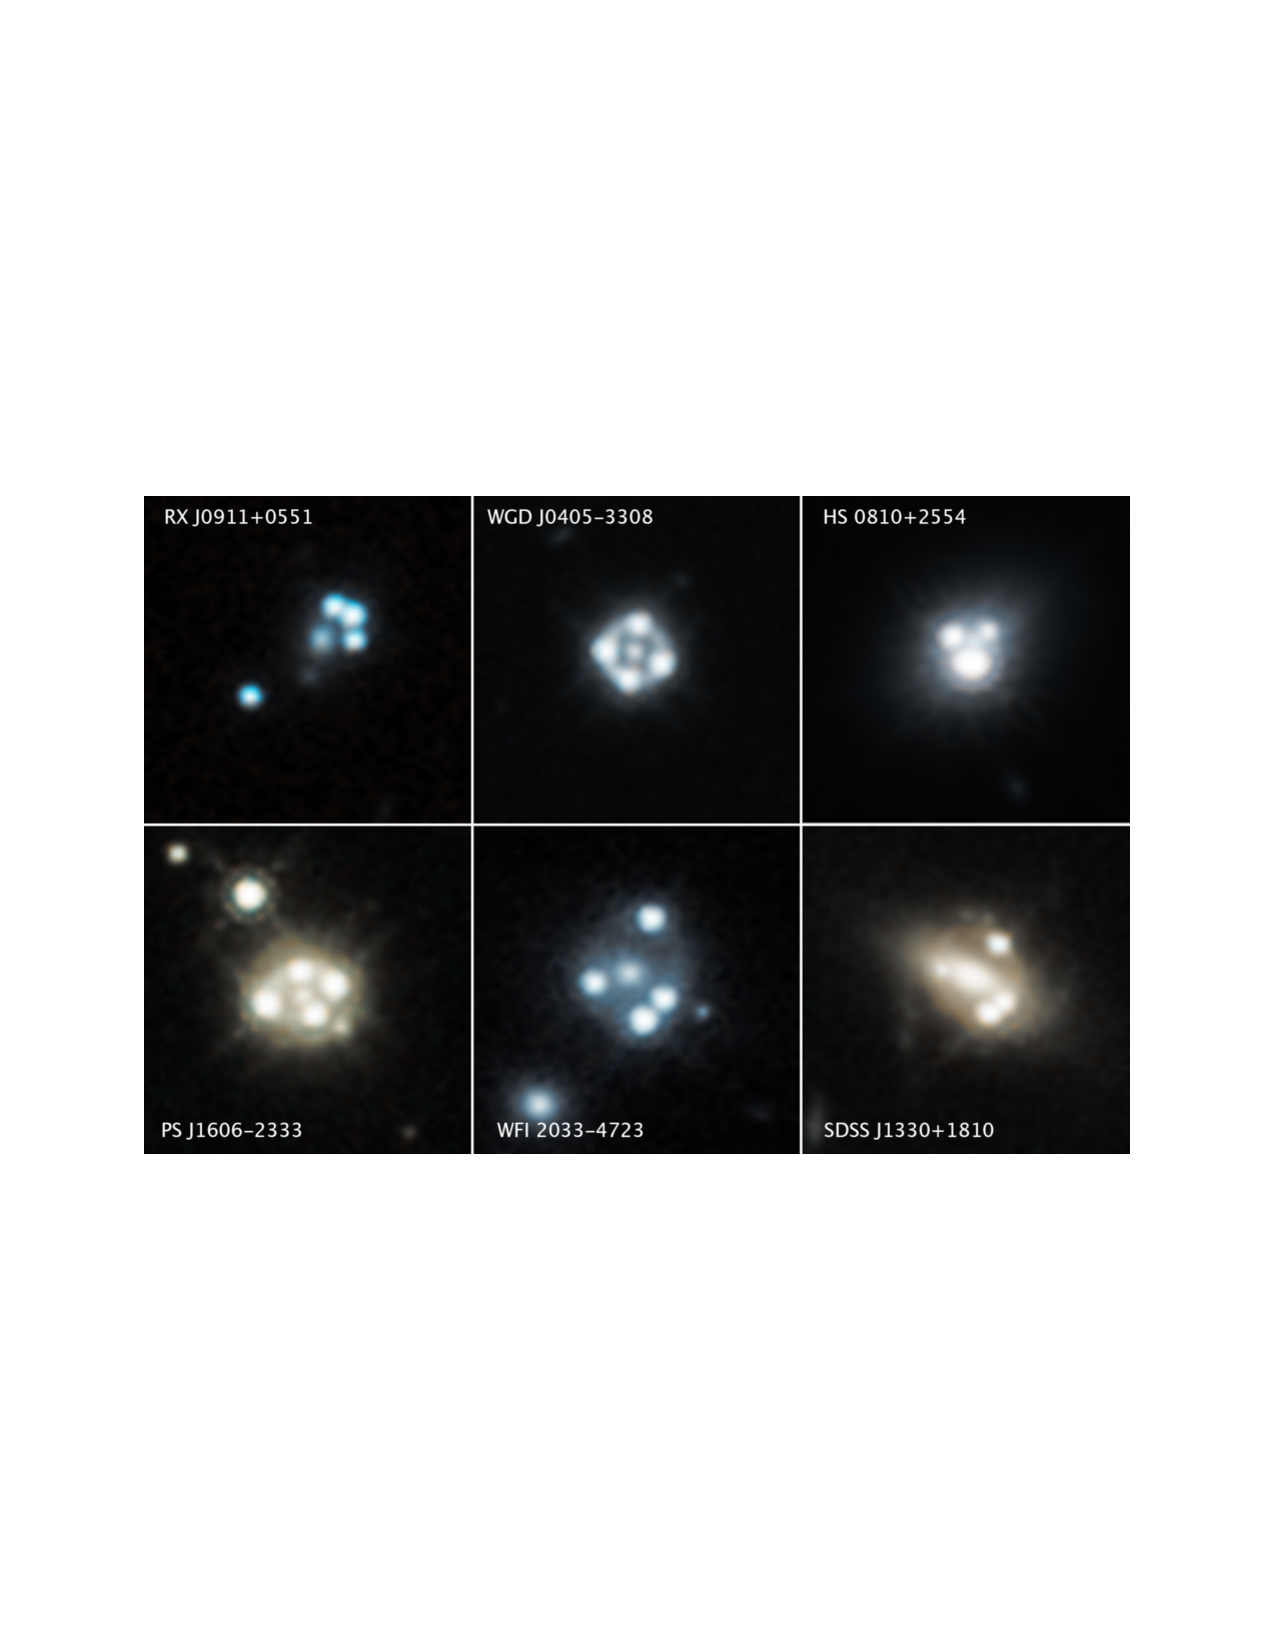
\includegraphics[clip,trim=2.5cm 8cm 2.5cm
	8.5cm,width=.95\textwidth,keepaspectratio]{./figures_introduction/lenses.pdf}
	\caption[Six images of strong gravitational lenses]{\label{fig:lens2033} Six quadruple-image strong gravitational lens systems imaged by the Hubble Space Telescope \citep{Nierenberg++19}. The main lensing galaxy is visible as the faint object encircled by four highly-magnified images of a background quasar. Image credit: NASA, ESA, A. Nierenberg (JPL) and T. Treu (UCLA)}
\end{figure*}	
In this dissertation, I describe research that constrains particle theories of dark matter with strong gravitational lensing. The following sections of this introduction set the stage for Chapters 2-6, which describe the development and implementation of a technique to constrain any dark matter model using the image magnifications from a sample of quads. Section 1.1 begins with a review of how the particle nature of dark matter drives structure formation in the Universe, and what aspects of structure formation lensing can constrain. Next, I review the basic theory connecting dark matter structure to lensing observables. 

\section{Structure formation and dark matter physics}
\indent An initially diffuse field of dark matter particles will collapse into gravitationally-bound halos through a mechanism called `violent relaxation' \citep{LyndenBell67}. The halo mass function, or the number of halos per unit mass, encodes information about when the first dark matter halos collapsed in the early Universe. Similarly, the density profiles of individual halos as a function of mass, the mass-concentration relation, depends on the hierarchical assembly of dark matter halos through cosmic time, and the shape of the primordial matter power spectrum that seeded the growth of structure. The particle nature of dark matter affects both the initial matter power spectrum and the growth of density fluctuations initialized at early times, imprinting clues regarding the particle nature of dark matter in the large and small-scale structure of the Universe. 

As a concrete example, consider two competing classes of dark matter models: Cold, and Warm Dark Matter (CDM and WDM, respectively). A quantity called the free-streaming length $\lambda_{\rm{FS}}$ distinguishes these two models. By definition, free-streaming effects are negligible in CDM. In WDM scenarios, diffusion of dark matter particles out of potential wells initialized in the early Universe wipes out small-scale density fluctuations. This diffusion process transforms a density field initialized with a scale-free power spectrum $P\left(k\right) \propto k^{n}$ into a density field with a power spectrum truncated at a scale $k_{\rm{FS}} = \frac{2 \pi}{\lambda_{FS}}$. The characteristic length scale $\lambda_{\rm{FS}}$ can be approximated as the comoving distance a particle could have traveled before structure begins growing in earnest around the time of matter-radiation equality $t_{\rm{EQ}}$ \citep{Schneider++12} 
\begin{figure}
	\centering
	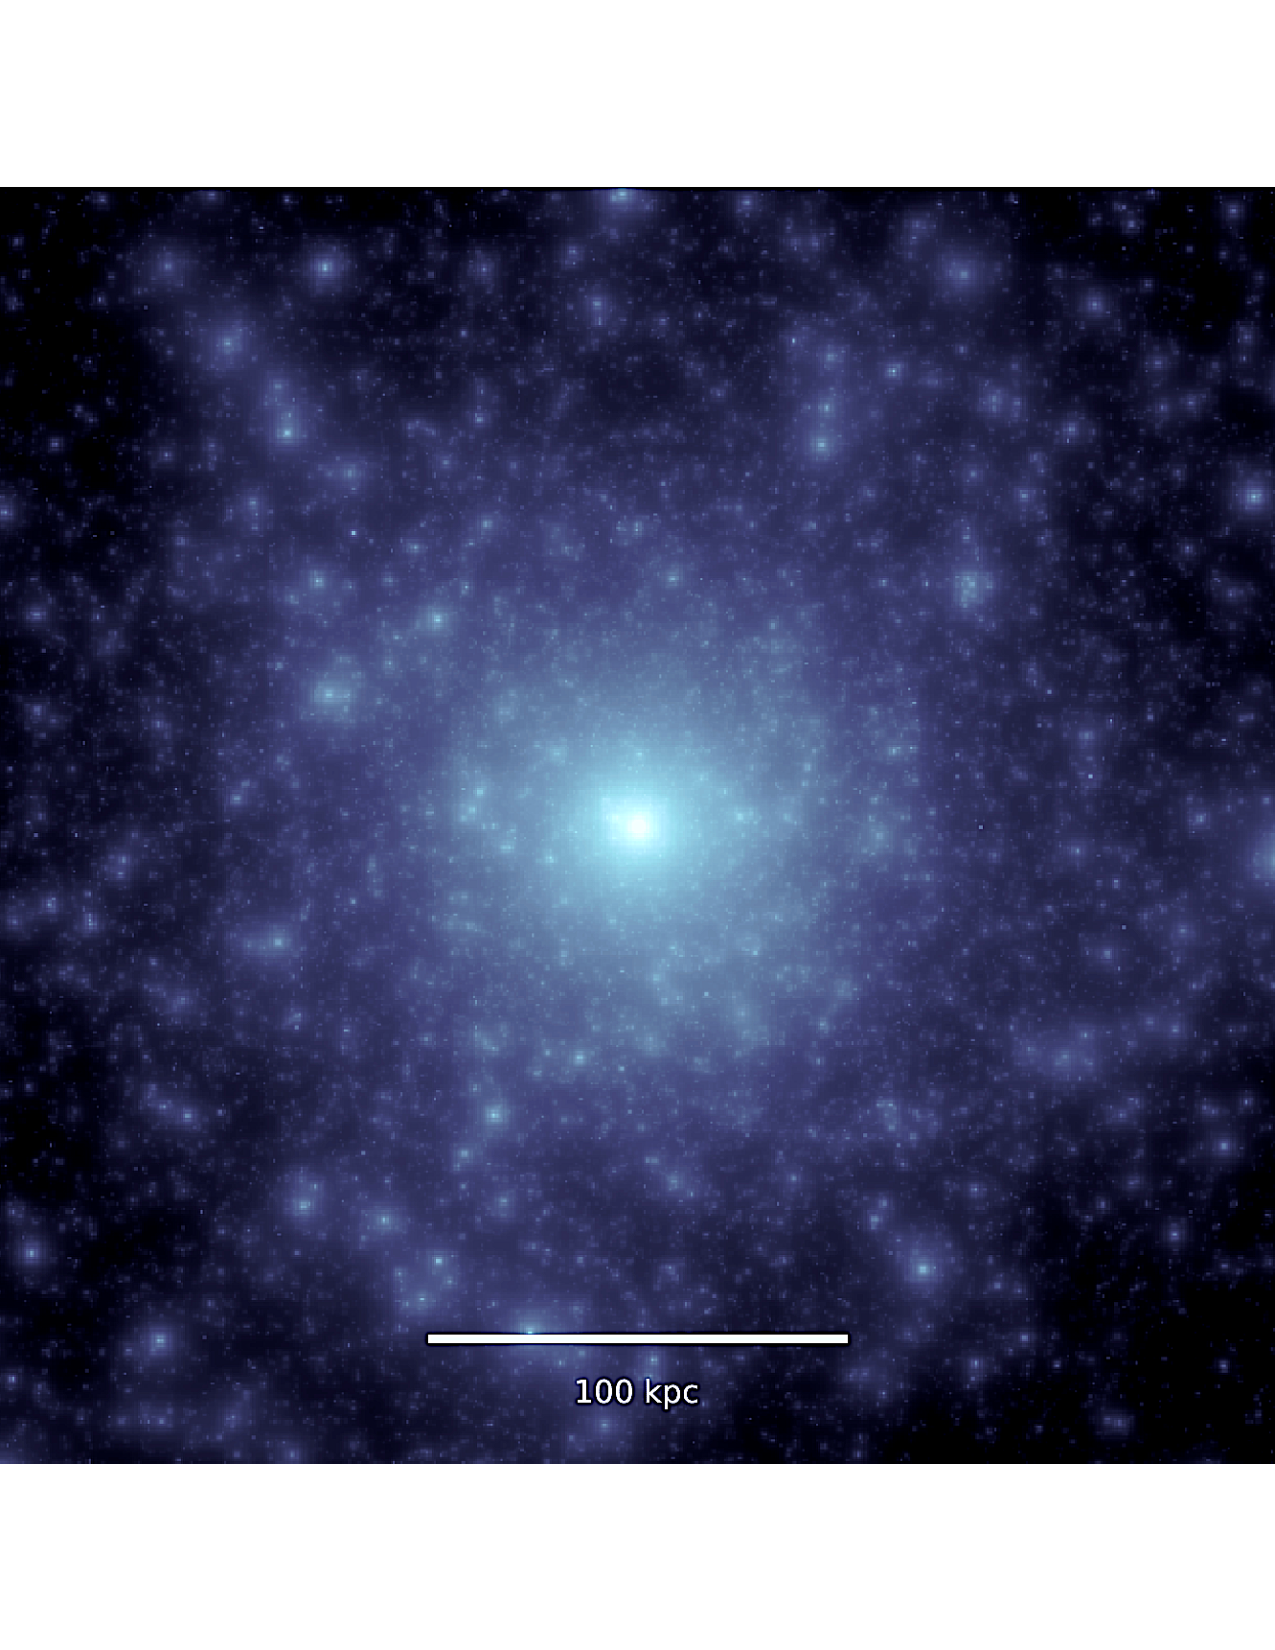
\includegraphics[clip,trim=0cm 0cm 0cm
	0cm,width=.49\textwidth,keepaspectratio]{./figures_introduction/CDMscreenshot_edited.pdf}
	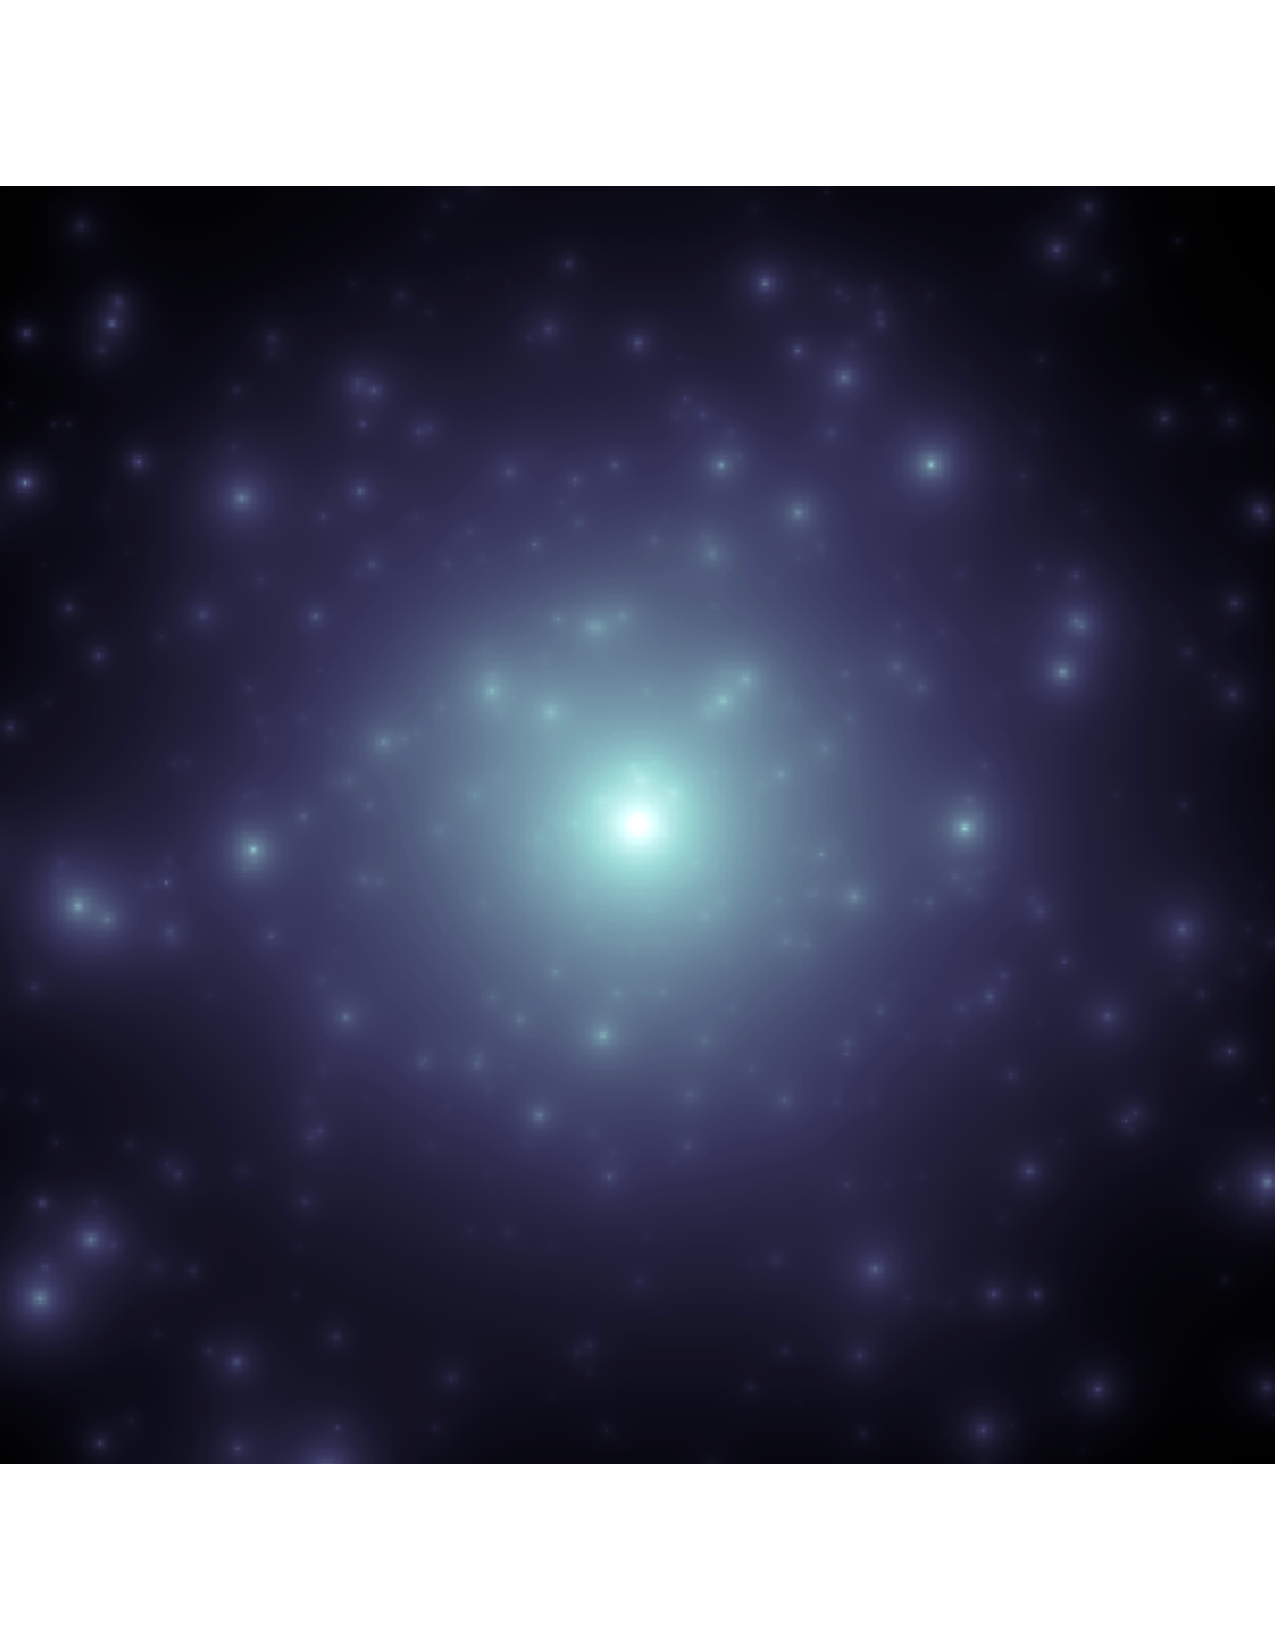
\includegraphics[clip,trim=0cm 0cm 0cm
	0cm,width=.49\textwidth,keepaspectratio]{./figures_introduction/WDMrealization_nobar.pdf}
	\caption[CDM and WDM subhalo populations]{\label{fig:wdmrealization} {\bf{Left:}} A realization of CDM substructure, with a scale-free subhalo mass function. {\bf{Right:}} A realization of WDM substructure corresponding to a $3.3 \rm{keV}$ thermal relic dark matter particle, which produces a turnover in the halo mass function around $10^8$ solar masses. }
\end{figure}

\begin{equation}
\label{eqn:freestreaming}
\lambda_{FS} \approx \int_{0}^{t_{\rm{NR}}} \frac{c dt}{a\left(t\right)} +  \int_{t_{\rm{NR}}}^{t_{\rm{EQ}}} \frac{v\left(t\right) dt}{a\left(t\right)} \approx r_{H}\left(t_{\rm{NR}}\right) \left(1 +\frac{1}{2} \log \frac{t_{\rm{EQ}}}{t_{\rm{NR}}} \right),
\end{equation}
where the particle has speed $c$ before becoming non-relativistic at time $t_{NR}$, $r_H \left(t_{\rm{NR}}\right)$ is the comoving horizon size at $t_{\rm{NR}}$, $a\left(t\right)$ is the cosmological scale factor, and $v\left(t\right)$ represents the average velocity distribution of the dark matter particles\footnote{This expression assumes that the particles become non-relativistic before $t_{\rm{EQ}}$, and uses the fact that $a\left(t\right)\propto t^{\frac{1}{2}}$ before $t_{\rm{EQ}}$.}. 

The effects of free-streaming manifest in structure formation in two ways: First, erasing small-scale power at early times eliminates the small-scale density fluctuations in the primordial matter density field that would eventually collapse into the smallest dark matter halos. This suppression of small-scale power results in a turnover in the halo mass function at a certain mass scale that is proportional to the $k_{\rm{FS}}^{-3}$ \citep{AvilaReese++01,Schneider++12,Lovell++14}. Second, because low-mass halos collapse first in hierarchical structure formation scenarios, eliminating the smallest halos delays the onset of structure formation. As the central density profile of a dark matter halo reflects the background density of the Universe at the time of collapse, delaying structure formation suppresses the central density of dark matter halos. Mergers between low-mass halos into larger halos propagate these effects to larger halo masses, affecting structures over an order of magnitude in mass above the scales that are directly impacted by free-streaming effects \citep{Navarro++96,Bose++16}. These structure formation arguments apply to both isolated halos in the field, and subhalos of the $10^{13}$ solar mass host dark matter halos that contain early-type galaxies typically acting as strong lenses \citep{Gavazzi++07}. The left and right panels of Figure \ref{fig:wdmrealization} show examples of CDM and WDM subhalo populations, respectively. 

The dependence of $\lambda_{FS}$ on features such as $t_{NR}$ and $v\left(t\right)$ links the free-streaming length of the dark matter to the formation mechanism and velocity distribution of the dark matter particle(s). As the halo mass function and mass-concentration relation depend on the free-streaming length, it follows that constraining the halo mass function and halo density profiles can be cast as a constraint on fundamental dark matter physics determining $t_{NR}$ and $v\left(t\right)$. Notice, however, that none of the previous discussion depends on a particular choice dark matter particle. We can simultaneously rule out neutrinos, thermal relics with mass $< 2 \rm{keV}$, and sterile neutrinos produced via Higgs decay with a mass of $7 \rm{keV}$ \citep{Viel13,AbazaijanKusenko19} making up 100$\%$ of the dark matter, as the free-streaming lengths corresponding to each these models precludes the formation of galaxies such as the Milky Way. Properties like the free-streaming length can be computed for practically any model in the literature, illustrating the broad scope and power of structure formation arguments. 

In order to employ structure formation arguments, one requires a method to detect, and measure the mass of, dark matter halos. One approach uses the fact that galaxies are believed to reside inside dark matter halos; luminous structures, such as galaxies, therefore trace the underlying dark matter. Unfortunately, the approach of using luminous matter as a proxy for invisible halos becomes increasingly difficult below $10^9$ solar masses, as not every halo on these scales hosts a visible galaxy. Moreover, uncertainties that stem from astrophysics on sub-galactic scales that determine how one assigns a dark matter halo mass to an observed galaxy can sometimes be larger that the differences between predictions from the dark matter models of interest \citep{Nierenberg++16}. While recent advances in this field make considerable progress towards appropriately dealing with these complications \citep{Nadler++19}, the systematic uncertainties persist. A second technique to probe small-scale structure in the Universe relies on the flux power spectrum of the Lyman-$\alpha$ forest at $z \sim 5$, which under certain assumptions can be used as a proxy for the matter power spectrum \citep{Viel13,Irsic++17}. The promise of this method must be weighed against the systematic uncertainties associated with thermodynamic processes relevant to the Lyman-$\alpha$ forest, which can mimic the suppression of small-scale power predicted in WDM scenarios \citep{Garzilli++19}. 

Strong gravitational lensing by galaxies offers an alternative, more direct probe of dark matter structure on scales below $10^8$ solar masses. Lensing couples only to gravity, and therefore circumvents the challenges associated with using baryonic matter to trace the underlying dark matter. In the next section, I review the formalism connecting lensing observables to populations of dark matter halos along the entire line of sight from the observer to the source. 

\section{Strong lensing signatures of dark matter halos}
\indent General relativity relates the deflection angle of a light ray to the mass distribution of a massive structure, dark or luminous. When the distances scales between the observer, lens, and source are much greater than the physical extent of the lensing mass distribution, the effect of a massive deflector can be approximated as a single sharp deflection in the plane of the lens, the `thin lens' approximation. Defining $\Sigma\left(\vec{\xi}\right)$ as the projection of a deflector's three dimensional density profile onto the plane of the lens at the coordinate $\vec{\xi}$, the deflection angle is given by \citep{BlandfordNarayan86}
\begin{equation}
\label{eqn:defangle}
\vec{\alpha}\left(\vec{\xi}\right) = \frac{4G }{c^2} \int \frac{\left(\vec{\xi} - \vec{\xi^{\prime}}\right) \Sigma\left(\vec{\xi^{\prime}}\right)}{| \vec{\xi} - \vec{\xi^{\prime}}|^2} d^2 \xi^{\prime}. 
\end{equation}
For multiple deflectors in a single lens plane, the cumulative effect is a linear superposition of their individual deflection angles $\vec{\alpha}$. 

A strong lens system will include both subhalos associated with the host dark matter halo of the lensing galaxy, and field halos distributed along the entire line of sight. Incorporating field halos requires the multi-plane ray tracing equation, which maps an angular coordinate on the sky $\vec{\theta_1}$ to an angular coordinate on the source plane $\vec{\theta_s}$. The ray tracing equation that determines where images appear to the observer is given by \citep{BlandfordNarayan86}
\begin{equation}
\label{eqn:raytracingintro}
\vec{\theta_s} = \vec{\theta_1} - \frac{1}{D_{\rm{s}}} \sum_{i=1}^{s-1} D_{\rm{is}}{\vec{\alpha_{\rm{i}}}} \left(D_{\rm{i}} \vec{\theta_{\rm{i}}}\right),
\end{equation} 
where the net deflection angle from all halos at the $i$th lens plane can be computed with Equation \ref{eqn:defangle}, $D_{\rm{ij}}$ is the angular diameter distance from the $i$th lens plane to the $j$th, and subscript $s$ identifies the source plane. Equation \ref{eqn:raytracingintro} is a recursive equation for the position of deflected light rays at each lens plane. It describes a physical process similar to viewing an image through multiple magnifying glasses in series, coupling deflections produced by objects at different distances. 

As gravitational lensing conserves surface brightness \citep{MisnerThorneWheeler}, the (de)magnification of the lensed images is proportional to the ratio of areas in the image and source planes. This factor is computed from the inverse determinant of the jacobian $\left(\det \frac{\partial \vec{\theta_s}}{\partial \vec{\theta_1}}\right)^{-1}$. While the full expression for the lensing jacobian in the general multi-plane framework (see \citet{BlandfordNarayan86}) is long and not particularly illuminating, the key point is that the magnification of an image depends non-linearly on derivatives of the lensing deflection angle. Image magnifications are therefore highly localized probes of the mass distribution along the line of sight to strong lenses. While the exact level of perturbation to an image magnification depends on the size of the background source, the mass of the halo, and the position of the image relative to the critical curve, a dark matter halo as small as $10^7 M_{\odot}$ near a lensed image can induce measurable perturbations on image magnifications for background sources of size $O\left(10\right)$ pc. 

The idea that dark matter halos frequently perturb image magnifications was first put forward in 1997 \citep{MaoSchneider98}. Since that time, authors have attributed lensing `flux anomalies', or the consistent failure of smoothly-parameterized mass distributions to reproduce the magnifications ratios observed in quad lens systems\footnote{Since the intrinsic brightness of the source is unknown, the observable quantity is the magnification ratio, rather than the magnification itself.}, to the presence of substructure in the lens system \citep{Metcalf++02,D+K02,FadleyKeeton12,Xu++12,Nierenberg++14,Nierenberg++19}. Early studies of strong lensing flux anomalies (e.g. \citet{D+K02}) relied on lensed radio emission from the background quasar. This technique has drawbacks that are remedied by the advent of nuclear narrow-line emission from the background quasar as probe of substructure, a method first proposed by \citet{MoustakasMetcalf02}, and subsequently implemented by \citet{Sugai++07,Nierenberg++14,Nierenberg++17,Nierenberg++19}. The use of lensed narrow-line emission has two advantages: First, the nuclear narrow-line region is spatially extended by $\sim 50$pc \citep{MullerSanchez++11}, preventing contamination from microlensing and variability in background source brightness\footnote{The light crossing time of the narrow-line region washes out the small-scale variability in the light curve of the background source.}, processes that considerably inflate uncertainties in radio flux ratios. Second, narrow-line emission is present in the spectrum of virtually every quasar, expanding the sample size of available lens systems. Recently, the sample size of strong lens systems with measured narrow-line flux ratios increased by nearly a factor of four \citep{Nierenberg++19}. 

During my PhD, I developed a flexible and powerful Bayesian inference framework that takes full advantage of flux ratios measured using nuclear narrow-line emission to constrain any dark matter model, provided the model predicts the shape of the halo mass function, and the density profile of individual halos. The methods I developed improve over previous work in two key ways: First, they account for halos along the line of sight to strong lenses, which can sometimes outnumber the subhalos associated with the main deflector. Second, the method naturally accommodates spatially extended background sources, which affect the sensitivity of lensing observables to dark matter halos. The tools I developed delivered one of the tightest constraints on the free-streaming length of dark matter to date (see Chapter 5), independent of and more stringent than those obtained from the Lyman-$\alpha$ forest \citep{Viel13}, and the first observational constraint on the mass-concentration relation of CDM halos on sub-galactic scales across cosmological distance (see Chapter 6). 

This dissertation is organized as follows: Chapter 2 describes a study that quantifies the intrinsic uncertainty associated with smoothly-parameterized lensing mass profiles, irrespective of the dark matter substructure content of the lens system. Chapters 3 and 4 describe the development and testing of the analysis framework I developed to combine a sample of strong lenses to constrain dark matter models. Finally, in Chapters 5 and 6 I present results obtained using methods I developed, constraining free-streaming length of dark matter, and the mass-concentration relation of CDM halos, respectively. 

%\bibliography{bibmaster} 
%\bibliographystyle{uclathes}
% \section{Related Work}
%	\label{sec:intro_related_work}

% ...


% LocalWords:  Posix Novell's Netware Kernighan Madnick Alsop NeFS PostScript
% LocalWords:  Rosenthal SunSoft NEEDSWORK Wong

%\def\kex{{\kappa_{\rm e}}}
\def\RE{{R_{\rm E}}}
\def\Reff{{R_{\rm eff}}}
\def\gd{{\gamma_{\rm d}}}
\def\fd{{f_{\rm dm}}}
\def\ra{{r_{\rm a}}}

\chapter{Strong lensing signatures of luminous structure and substructure in early-type galaxies}
\textit{This chapter was published as Gilman, D., et al. Strong lensing signatures of luminous structure and substructure in early-type galaxies. MNRAS 467, 3970-3992 (2017), and is printed here with minor formatting adjustments.}

\section{Introduction}

One of the most robust predictions of cold dark matter models is that
galaxy and cluster scale halos should host a large number of subhalos,
described by a steep mass function of the form $dn/dM\propto M^{-1.9}$ \cite{Klypin++99,MaoSchnieder98}. Observational evidence against this prediction would force a revision of the standard model in favor of more exotic kinds of dark matter. For example, dark matter models with non-negligible free streaming lengths, such as keV scale sterile neutrinos are expected to manifest as a cutoff in the subhalo mass function \cite{Colombi++96,Vogelsberger++16,Bose++16,Lovell++16,Menci++16}.

The standard test of this prediction consists of measuring the abundance of luminous satellites around galaxies such as the Milky Way. Significant efforts over the past decades have shown that indeed the abundance of luminous satellites is lower than what is predicted for subhalos. However, the interpretation of this tension is ambiguous. Low mass subhalos might not exist in sufficient numbers, or could simply not be capable of forming stars, and thus be invisible \cite{Nierenberg++14,Nierenberg++16,Gao++11,Starkenburg++13,Wetzel++16,Sawala++16,DespVeg16}.

For almost two decades it has been recognized that strong gravitational lensing offers an alternative and potentially very clear observational test of this fundamental cosmological prediction, whereby the properties of dark matter subhalos are probed directly by their impact on the arrival times, positions, and flux ratios of lensed images. A variety of techniques have been developed over the years to carry out these measurements, and applied to a variety of datasets. Broadly speaking, the measurements obtained so far are consistent with cold dark matter predictions, although their sensitivity has been limited by sample sizes and quality of the data. Fortunately, sample size and data quality are rapidly improving, and it is therefore important to explore all sources of potential systematic errors in the applications of this technique.

The goal of this paper is to study the impact of baryonic substructure on the application of the so-called lensing anomalies (in time delays, positions, and fluxes) to the study of dark matter substructure.  The term anomalies arises from the standard approach in strong lensing communities where the mass distribution of a galaxy is described as the superposition of a `smooth' mass distribution representing most of the luminous and dark matter, plus a clumpy distribution of dark substructures typically in the range $10^6 - 10^9 M_{\odot}$. This approach is motivated by the fact that a simple smooth component is generally sufficient to capture the main features of the lensing observables, while substructure below a certain threshold effectively behaves as smooth for given bakcground source size.

Typically, the positions and arrival time delays between lensed images are reproduced by a smooth lens model, while the ratios of the magnifications (also known as flux ratios) may or may not be recovered \cite{MetcalfMadau01,D+K02,Bradac++04,Xu++09,Xu++15}. If the observed flux ratios cannot be recovered with `smooth' lens models, the flux ratios are deemed anomalous, and the discrepancy is attributed to the presence of a compact, massive perturbing mass near an image, such as a dark subhalo. Similarly, the inability of smooth models to reproduce image arrival times and astrometry (both for compact and extended sources) gives rise to the so-called time delay and astrometric anomalies \cite{Chen++07,KeetonMoustakas09}. Both astrometric and flux ratio anomalies have been used to characterize the distribution, abundance, mass function, and density profile of subhalos \cite{MetcalfMadau01,D+K02,Chiba02,Vegetti++09,Vegetti++12,FadleyKeeton12,Veg++14,Nierenberg++14,Hezaveh++16}.

However, the presence of dark subhalos is not the only possible explanation for the observed anomalies.  Stellar microlensing \cite{Schechter++03} and matter along the line of sight \cite{Metcalf05,Xu++12} can give rise to anomalies in the positions and flux ratios of compact sources. The astrophysical noise from these features can be mitigated by observing sources that are sufficiently extended to smooth away microlensing, by observing at wavelengths unaffected by dust, and by carrying out multiplane lensing analysis.

In this study we focus on astrophysical noise arising from inhomogeneities in the stellar mass distribution of the lensing galaxy that may not be resolved at typical lens redshifts, and could potentially cause anomalies that could be conflated with the presence of dark subhalo. A clear and recent example is given by \cite{Hsueh++16}, who show that the apparent flux ratio anomaly in the system B1555 can be readily explained by the presence of an elongated disk in the deflector, which is detected in high resolution imaging of the system.

This potential noise term was recognized early on. For example, \cite{MaoSchneider98} and \cite{Chiba02} calculated the impact of globular clusters based on simple analytic models. \cite{Moller++03} highlighted the importance of disk components in the statistics of flux ratios, considering their occurrence in early-type galaxies within nearby galaxy clusters. With improvements in sample size and data quality it is important to revisit theses issues and perform quantitative, systematic, and realistic calculations of the overall distribution of the anomalies induced by the stellar component on arrival times, positions, and fluxes of the multiple images. In this context, using numerical simulations, \cite{Xu++10} have shown that the density profiles in the vicinity of the Einstein radius of simulated galaxies are not as simple as those traditionally used to model galaxy-scale lenses, which could amplify the impact of the baryonic mass component of a lens.

In this work, we address this problem by using real Hubble Space Telescope (HST) observations of nearby galaxies to build mock lenses with realistic baryonic mass distributions, and varying degrees of morphological complexity.  We complement this baryonic mass component with an NFW dark matter halo, omitting dark substructure in order to isolate the effect of luminous matter. From the degree to which flux ratios from our mock lenses can be recovered with smooth lens models, we quantify the anomalies that can be attributed to the baryonic mass of a deflector (we identify stars with baryons but neglect the contribution of gas, which is assumed to be smooth on the relevant scales). 

This paper is structured as follows. In Section~\ref{sect:setup}, we detail our procedure for building mock lenses from HST images of nearby galaxies, the type of lens models considered in this work, and our fitting methodology. In Section~\ref{sect:results}, we present the results of our comparison between smooth models and realistic simulated lenses.  In Section~\ref{sect:conclusions}, we summarize the results of our analysis, and discuss the lessons learned in the context of ongoing and future strong lensing studies of dark matter.  
When needed to compute distances, we adopt a standard concordance cosmology with $\Omega_m=0.3$,  $\Omega_{\Lambda}=0.7$ and $h=0.7$, even though our results are independent of this choice. All of the lens simulations, ray-tracing and computation of lensing observables (positions, time-delays, magnifications) are performed using the {\tt{lensmodel}} software \cite{Keeton2011}.

\section{Building and fitting mock lens systems}
\label{sect:setup}

In this Section we describe in detail our procedure to build mock lens
systems and then fit them with lens models. We begin by describing our
source of high resolution images about the surface brightness of
early-type galaxies in Section~\ref{ssec:sb}. In
Section~\ref{sect:lenses} we summarize how we obtain the global
structural parameters for the lens galaxies, either from the
literature or our own fits to the light. In Section~\ref{ssec:tomass} we describe
how we convert surface brightness into lensing potential, accounting
for the dark matter halo and external shear. In
Section~\ref{ssec:models} we describe the ingredients of our five
different mass models used to produce mock lenses and fit them. In
Section~\ref{ssec:mocks} we describe the process of generating data sets with our mock lenses for two of our models that are derived from the real HST images, and in Section~\ref{sect:fitting} we describe the process of fitting two smooth lens models to data obtained from the mock lenses.

\subsection{The stellar surface brightness of early-type galaxies at high resolution}
\label{ssec:sb}

The starting point for our mocks is archival Hubble Space Telescope observations early-type galaxies from the nearby Virgo and Coma clusters \cite{Ferrarese++06,COMAsurvey08}. In order to obtain a sample that is representative of lensing galaxies we select all the elliptical and lenticular galaxies with available HST images, central velocity dispersions between 165 and 320 km s$^{-1}$, and ellipticities in the range 0.05-0.43. We limit our selection to galaxies imaged with the Advanced Camera for Survey with filters F814W or F850LP, in order to minimize the effects of dust, and map the stellar light as closely as possible, while taking advantage of the wider field of view of view and finer pixel scale than the infrared channel of Wide Field Camera 3. The sample displays a variety of interesting features, including globular clusters, disks, tidal tails and shells, which we take as representative of the kind of baryonic structure and substructure that we are interested in studying. In Table~\ref{table:gal_list}, we list the galaxies used in our data set, along with their relevant physical parameters.

We avoid galaxies with prominent dust lanes, and sources of visual contamination obvious to the naked eye, as these features would be problematic in our procedure for assigning mass to light, which we discuss in the next section. There are often bright galaxies or stars in the line of sight, which we replace with a smooth interpolation of the main lens profile. We do not expect this to significantly affect our results, however, as we avoid generating lenses where an image would be located near one of these defects. When the computation of the lensing potential, according to our normalization procedure, requires information from pixels outside the ACS field of view, we extrapolate a smooth model fit to the light into these regions. After solving the lens equation, we ensure that no lensed images land in an interpolated region.

We note that real lens samples tend to be dominated by high velocity dispersion galaxies above 240 kms$^{-1}$\cite{Auger++10,Son++13a}, due to their favorable lensing cross section. Surveys of high velocity dispersion galaxies \cite{Goulding++16} show that the most massive ellipticals tend to be slow rotators, while low velocity dispersion galaxies, which are more likely to be fast rotators and host disks, are over-represented in our mock sample. As such, our sample is not representative of that of typical lens galaxies, and will likely result in an over-estimate of the contribution to time delay, astrometric, and flux ratio anomalies by the baryonic mass component of a deflector. In light of this, we interpret the fraction of anomalous systems in our analysis as an upper limit to the frequency with which one expects to encounter baryon-induced anomalies in a survey of real lensed quasars.
\begin{figure*}
	\centering
	{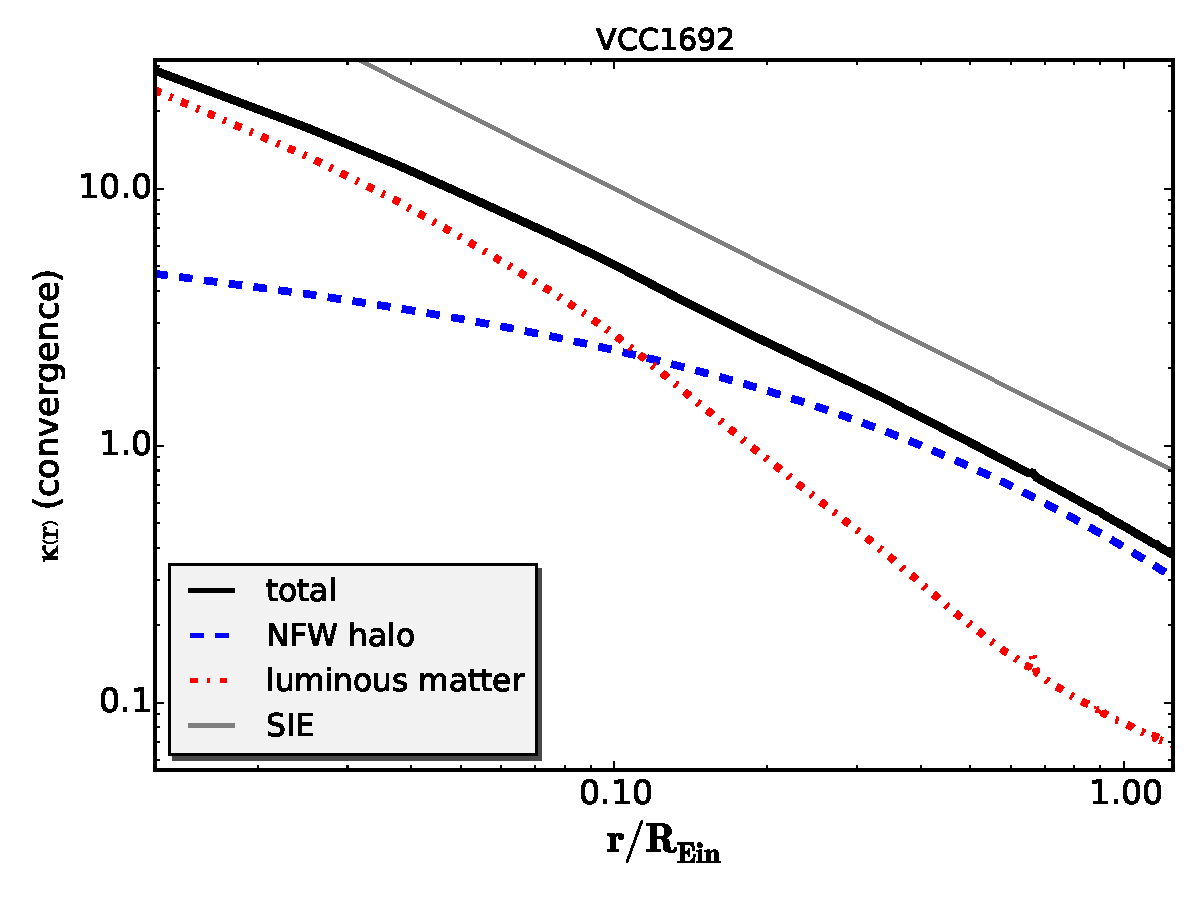
\includegraphics[trim=0.25cm 0.6cm 0cm
		0cm,clip,width=.48\textwidth]{./figures_sls/VCC1692r_vs_kap-eps-converted-to.pdf}}
	{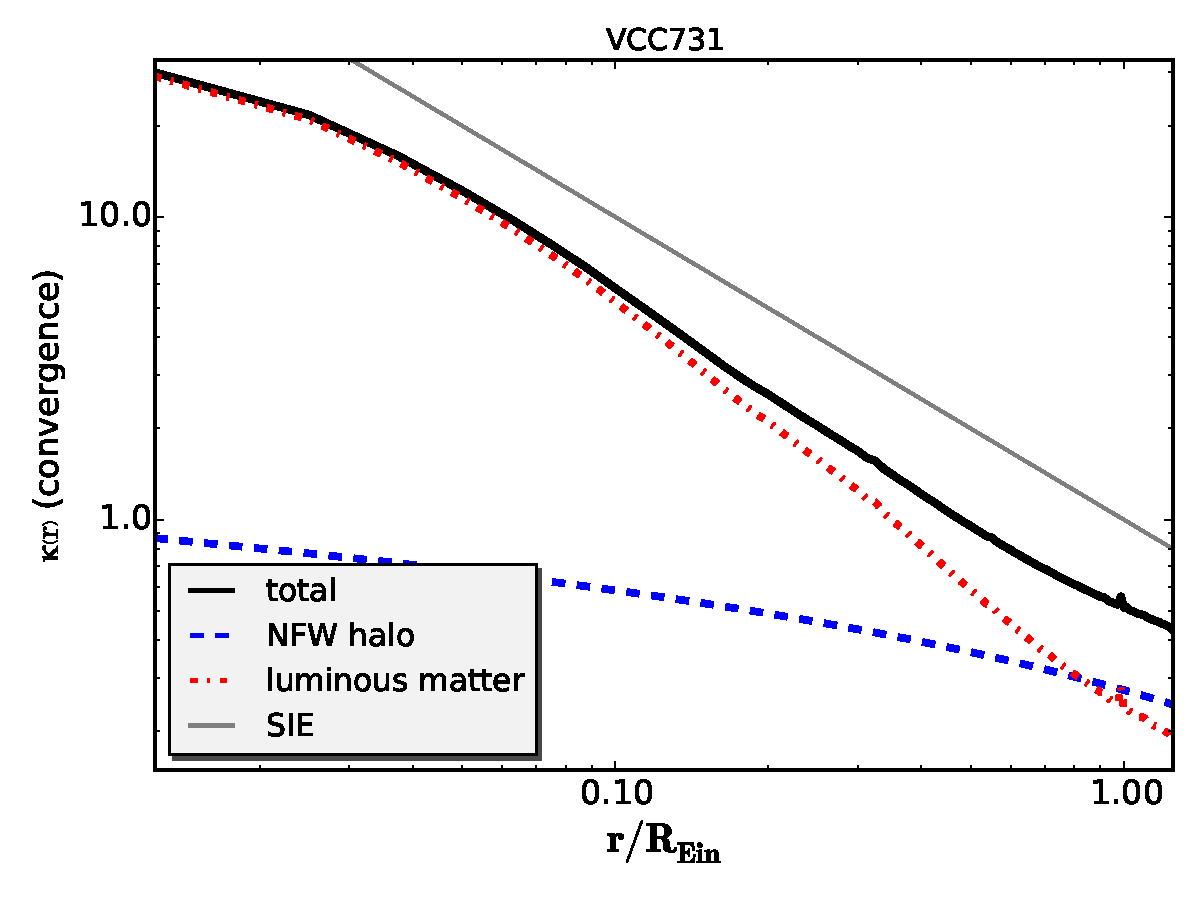
\includegraphics[trim=0cm .6cm 0cm
		0cm,clip,width=.48\textwidth]{./figures_sls/VCC731r_vs_kap-eps-converted-to.pdf}}
	\caption[Convergence as a function of radius for VCC1692 and VCC731]{\label{fig:r_vs_kap}Convergence as a function of radius for a normalized map of surface mass density for the deflectors VCC1692 and VCC731. For reference, the slope of an SIE mass density profile (with arbitrary normalization) is shown in grey.}
\end{figure*} 
\subsection{Structural Parameters of the Sample Galaxies}
\label{sect:lenses}

In order to simulate the lensing properties of the galaxies in our sample, we require a measurement of central stellar velocity dispersion $\sigma_*$, half-light radius $R_{1/2}$, ellipticity $\epsilon$, position angle $\theta_{\epsilon}$, and a S{\'e}rsic index $n$ for each host galaxy. We draw measurements of the central velocity dispersion from the HyperLeda online catalog \cite{Makarov++2014} and from \cite{Ma++2014}, while measurements of the half light radii, ellipticity and position we obtain for Virgo objects from \cite{Ferrarese++06} and from HyperLeda.

When the parameters describing the host light distribution are not available in the literature, we derive them by fitting the light profiles with a single S{\'e}rsic component using {\tt {galfit} } \cite{Peng++02} and derive the parameters ourselves, mimicking the efforts of an observer attempting to model the luminous matter of a strong lens. The parameters that we adopt for each galaxy are summarized in 
Table~\ref{table:gal_list}.

\subsection{From surface brightness to surface mass density}
\label{ssec:tomass}

We transform the surface brightness maps of the galaxies into maps of surface mass density (convergence) in order to determine the gravitational lensing properties. In translating between surface brightness and surface mass density, we assume that light traces luminous matter in the field of view, with a constant stellar mass-to-light ratio. This is a conservative approach as it will assign higher masses to young star populations which tend to populate disky areas, relative to the old star populations which tend to populate the smooth elliptical component. Thus, by adopting a uniform stellar mass to light ratio we tend to increase the lensing signal of disky structures, consistent with our interpretation of our results as upper limits on the perturbative effect of baryonic structure on lensing data. 

For simplicity, we simulate all our systems as they would be observed for typical deflector and source redshifts $z_{d}=0.5$ and $z_{s}=1.5$. The smooth dark matter component of each deflector is described by a circular NFW halo, whose scale radius $R_s$ is taken to be 5$R_{1/2}$, where $R_{1/2}$ is the half-light radius of the target galaxy, in projection. We do not expect this choice for the dark matter normalization to affect our main results, as our choice for $R_s$ simply reflects the different spatial scales over which the smooth dark matter and baryonic mass component vary. While real NFW halos are unlikely to be circular, the NFW halo in our analysis serves only to boost the convergence within the Einstein radius to that of a typical deflector. Further, ellipticity in the NFW halo is, to some extent, degenerate with external shear, which we add as a separate component.

We compute the Einstein radius of each mock lens by exploiting the observational fact \cite{Tre++06,Koopmans++09} that in lens galaxies the stellar velocity dispersion $\sigma_*$ approximates, within a few percent, the velocity dispersion $\sigma_{\rm{SIE}}$ of the best fitting singular isothermal ellipsoid (SIE), for which the Einstein radius is given by
\begin{equation}
R_{\rm E} = 4\pi\left(\frac{\sigma_{\rm{SIE}}}{c}\right)^2\frac{D_{ds}}{D_s},
\end{equation} 
where $D_s$, and $D_{ds}$ are the angular diameter distances to the source, and from the deflector to the source, respectively. This equation is one of the consequences of the so-called bulge-halo conspiracy \cite{TreuKoopmans02,TreuKoopmans04,Koopmans++06,Koopmans++09,DuttonTreu14}: the projected total mass density profile of early type galaxies is well described by a single power law with logarithmic slope $-1$. As a consistency check, we verify that the total convergence (after adding stellar mass to the light and a dark matter component) of our mock galaxies is well approximated by an isothermal profile, as shown in Figure~\ref{fig:r_vs_kap}. Also, we check that the stellar masses derived from our convergence maps are consistent with those reported by \cite{Gallo++08}. Details of the normalization procedure, based on empirical measurements of the relative abundances of stellar mass and dark matter, are given in Appendix~\ref{app:A}. 
In order to mimic the tidal field of the large scale structure expected at intermediate redshifts, we add, at random position angles, external shears of magnitude 0.05 or 0.08, which are typical shear magnitudes in strong lens systems \cite{HolderSchechter033}. 
\subsection{Description of the lens models}
\label{ssec:models}

In order to carry out our quantitative analysis of the lensing effects of unresolved stellar structures, we compare the lens configurations obtained from the high resolution mass maps (the ``truth''), with two models based on lower resolution data, and two simply parametrized smooth models commonly used in the literature. The two models based on a low resolution version of the ``truth'' are intended to simulate the best data that one could hope to extract from a distant lens using HST. The two simply parametrized lens models are meant to represent the models typically used as a reference to detect anomalies due to dark substructure.

Thus, in total, we consider five lens models, with the following
characteristics:

\begin{itemize}
	\item Model 1 (real data) - \textit{``Truth''}. This model directly uses the image of the galaxy obtained by HST, converted to a convergence map as described in the previous section and Appendix \ref{app:A}. 
\end{itemize}
\begin{figure*}
	\centering
	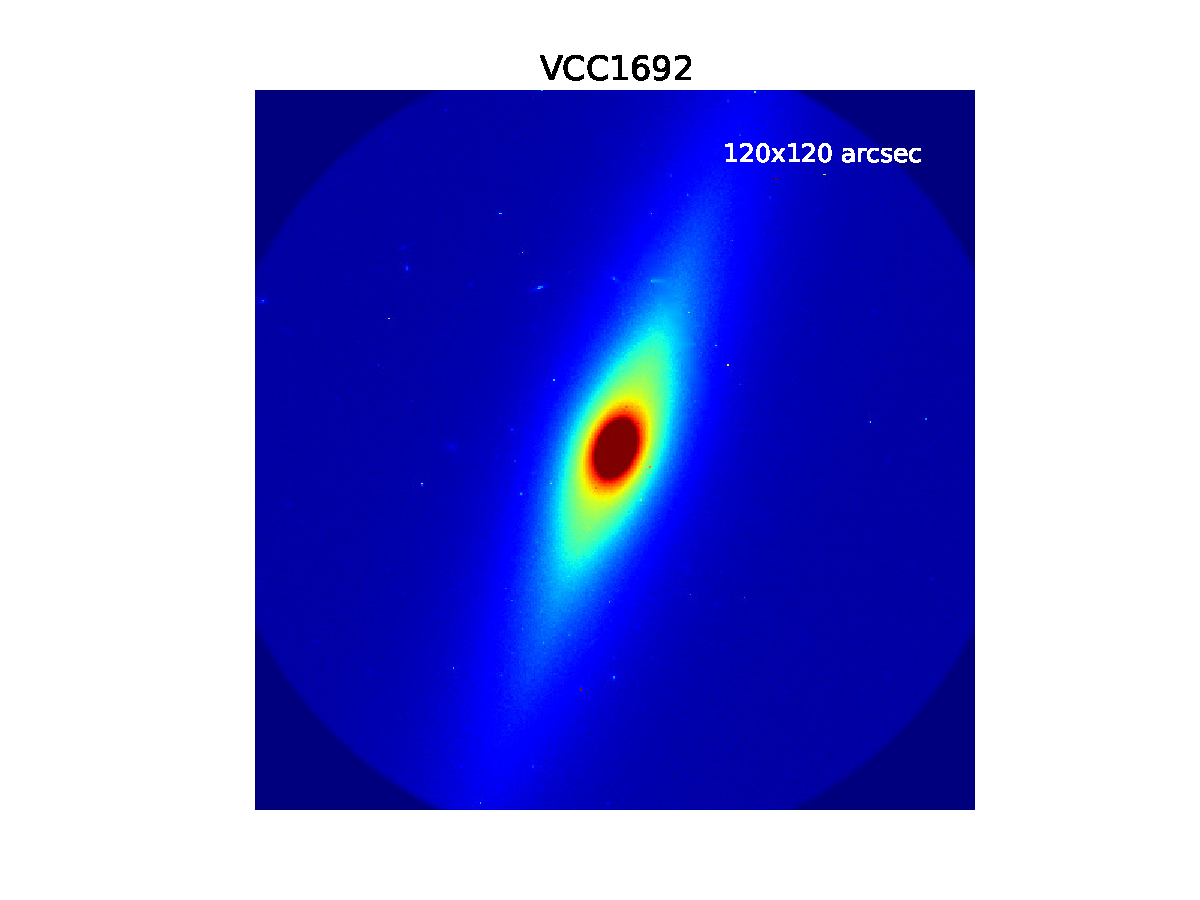
\includegraphics[clip,trim=4.1cm 1.5cm 4.1cm 2cm,width=.325\textwidth]{./figures_sls/baryonmap_truth-eps-converted-to.pdf}
	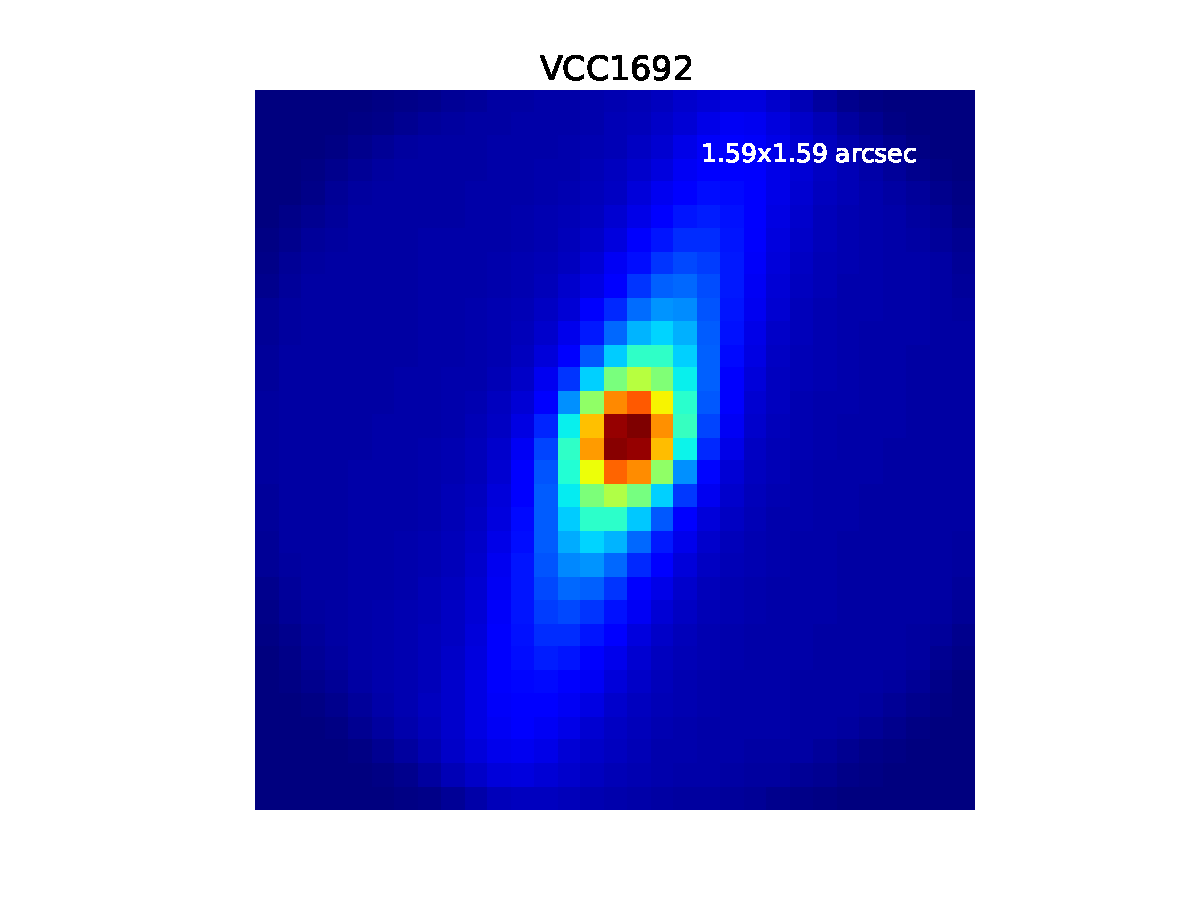
\includegraphics[clip,trim=4.1cm 1.5cm 4.1cm 2cm,width=.325\textwidth]{./figures_sls/baryonmap_RealHST-eps-converted-to.pdf}
	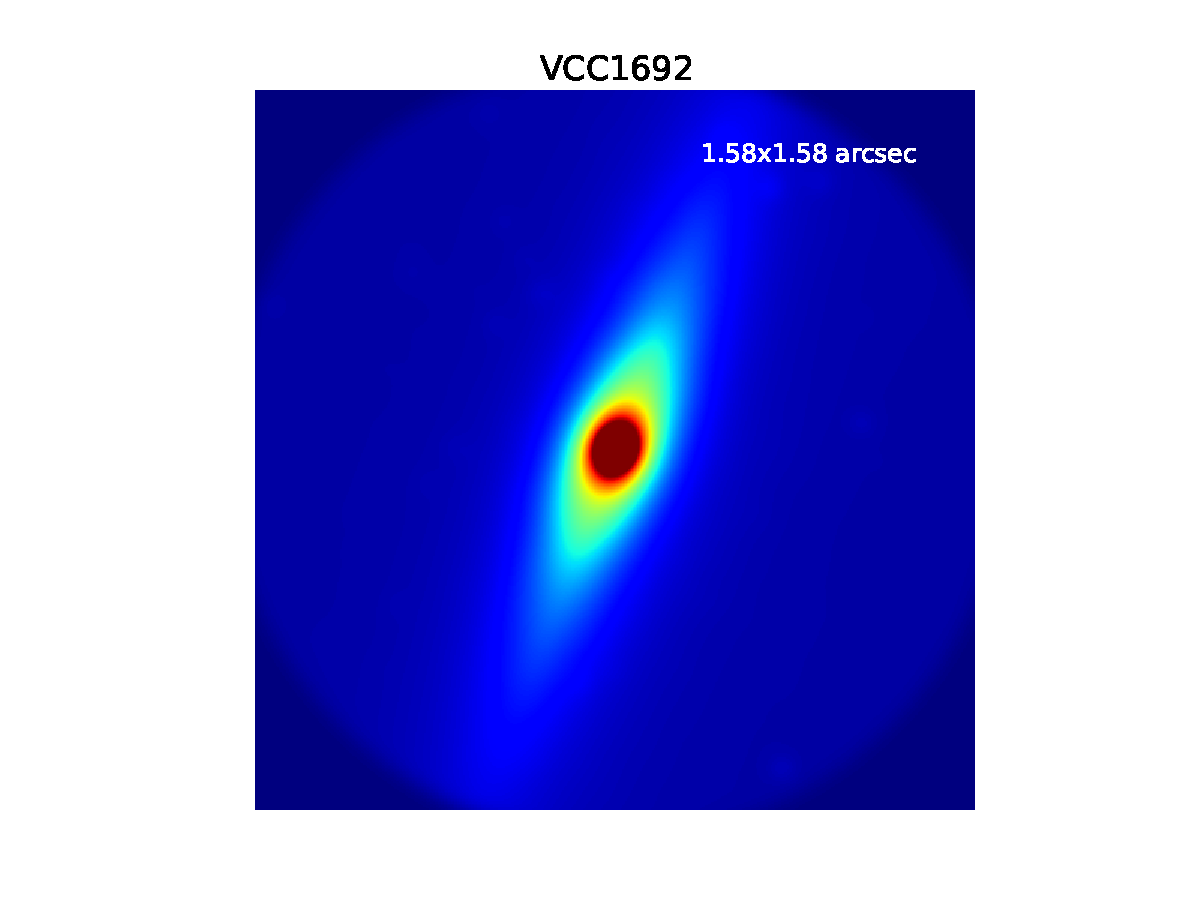
\includegraphics[clip,trim=4.1cm 1.5cm 4.1cm 2cm,width=.325\textwidth]{./figures_sls/baryonmap_smoothed-eps-converted-to.pdf}
	\caption[Maps of surface mass density]{\label{fig:VCC1692real_vs_mods}{\bf{\emph{Left:}}} Surface mass density of VCC1692 as it appears at a distance of 16 Mpc. \newline {\bf{\emph{Center:}}} The galaxy as it appears at redshift 0.5 (1280 Mpc) after rebinning pixels 80x80 to account for a loss of spatial resolution. \newline {\bf{\emph{Right:}}}  The galaxy after convolving with a Gaussian PSF with FWHM of 80 pixels (with pixel size the same as in far left panel, with resolution 0.05 arcsec pixel$^{-1}$) to simulate an observation of the galaxy where sub-pixel information has been recovered via dithering, effectively the best smooth model one could construct given HST data.}
\end{figure*}
\noindent We evaluate the following four models by their ability to reproduce the `real' data of Model 1:

\begin{itemize}
	\item Model 2 (relies on real data) - \textit{``real HST"}.  This is a simulated single exposure of an HST image, including the effects of a Gaussian PSF, and pixelization. First, we rebin pixels of the \textit{Truth} model by a factor corresponding to the loss of spatial resolution going to $z_d=0.5$ from the native redshift of the galaxy. For example, translating the angular diameter distance of the Virgo cluster ($z=0.0038$) to $z=0.5$ changes image resolution by a factor of 80, so the image used in the \textit{Truth} model is rebinned 80x80. We then convolve the rebinned map with a Gaussian Point-Spread-Function (PSF) of FWHM = 2 pixels. We checked that the order of operations of rebinning and convolving does not affect the results. This model is meant to represent an attempt to fit the stellar mass of the lens by scaling the pixel values observed by HST. An example is shown next to the \textit{Truth} stellar mass distribution in Figure~\ref{fig:VCC1692real_vs_mods}.
	
	\item Model 3 (relies on real data) - \textit{``HST Interpolated"}. This model simulates an HST image where the sub-pixel information has been recovered via dithering, thereby representing the best possible data set obtainable for these systems at a redshift of 0.5, approximating the Hubble PSF with a Gaussian PSF. In effect, this data has been smoothed over at a scale comparable to the Hubble PSF at redshift 0.5, thereby erasing structure on scales smaller than rebinning factor at redshift 0.5, thereby erasing structures on scales $<0.32$ kpc for Virgo galaxies, and $<0.51$ kpc for Coma galaxies. In practice, this model represents the best description of the stellar component that one could build from HST observations, using a smooth interpolation or a fit to the pixel data. As such, the degree to which this model reproduces the flux ratios from the \textit{Truth} model represents a noise floor for flux ratio data.  An example of the stellar mass distribution corresponding to this model is shown in Figure~\ref{fig:VCC1692real_vs_mods}.
\end{itemize}
The following two models are different from the previous three, as they are analytic functions fit to the data obtained from the \textit{Truth} model.
\begin{itemize}
	\item Model 4 (fit to \textit{Truth} positions, time delays) - Singular isothermal ellipsoid with external shear (SIE). This model is physically motivated by the fact that the combined mass profile of baryons and a NFW halo is well approximated by an isothermal power law, as shown in Figure \ref{fig:r_vs_kap}. We do not include information about image magnification when performing the fit, and use positional and time delay uncertainties of 0.003" and 2 days to simulate the best data currently available.
	\item Model 5 (fit to \textit{Truth} positions, time delays) - S{\'e}rsic + NFW halo (SNFW). We fit an elliptical S{\'e}rsic \cite{Sersic63} mass distribution and a NFW with external shear to image positions and time delays, with the same observational uncertainties as Model 4. The SNFW model has nearly double the number of free parameters as the SIE, which at face value suggests it would be a more adaptable functional form than the former, and better suited to representing a possibly complex distribution of baryonic and dark matter. However, models with too many free parameters are prone to degeneracies given the limited constraints available. We will consider this point again in Section 2.6. This model is meant to represent a practical approach which might be as close as possible to the best one can do, especially in the presence of bright lensed quasar images. 
\end{itemize}

We stress that because we do not explicitly add dark substructure to our mock lenses, the only source of small scale structures or non-smooth features, akin to the clumpy nature of dark matter substructure, is that of the baryons in the lensing galaxy, luminous satellites of the deflector, and background galaxies. Therefore, any discrepancy in flux ratios between the ``Truth'' model and models 4-5 is due entirely to a baryonic mass component that cannot be absorbed by the SIE or SNFW functions.

Similarly, with data of extraordinary quality, one could imagine using more flexible and complicated smooth lens models to describe the stellar mass component. This is captured in by the \textit{HST Interpolated} model, which provides a reasonable upper limit on the capability of a smooth lens potential to fully account for the baryonic structure of a lensing galaxy.

\subsection{Generating mock data sets}
\label{ssec:mocks}

For each of the three lens models based on real images (\textit{Truth}, \textit{Real HST}, \textit{HST Interpolated}), we manually place the source position within the astroid caustic so as to produce a cusp and a fold lens configuration. While the light traces mass hypothesis allows us to efficiently normalize and assemble realistic mock lenses, it introduces a significant complication. Shot noise in the HST images and discontinuities due to pixelization cause small scale variation in surface mass density that introduce a small scale pattern in the local magnification map. For a point source this would introduce a microlensing-like signal, which could introduce spurious scatter in the fluxes predicted by the \textit{Truth} model. We avoid this by modeling the background quasar as an extended source 5 parsecs in diameter, a procedure we describe in detail in Appendix~\ref{app:B}. For reference, this source size is roughly the size of a radio jet source (1-10 pc), but smaller than the narrow-line region (10-100 pc) \cite{MoustakasMetcalf02}, and is large enough to avoid micro-lensing effects while preserving sensitivity to small scale structure in the image plane, and corresponds to 0.265 mas$^2$ in the source plane.

For the three mock deflectors (Models 1-3), we apply a Monte Carlo procedure: for each image configuration (cusp and fold), we randomly sample 250 source positions from a circular area in the source plane, centered on a reference source position guaranteed to produce a cusp or a fold lens. For each of the 250 new source positions, for each of the \textit{Truth}, \textit{Real HST}, and \textit{HST Interpolated} convergence maps we directly solve the lens equation to obtain 250 new sets of positions, time delays, and flux ratios. We do not add measurement noise in this process, as we are only interested in the effects of baryonic mass on these data. 
\newline \indent For the simply parametrized lens models (Models 4 and 5), we use the software package {\tt{lensmodel}} to fit an SIE and SNFW model to each of the 250 data sets, corresponding to each of the 250 sampled source positions, constraining the models by only astrometric and time delay data and demanding that the S{\'e}rsic halo and NFW halo are centered at the same location. We introduce a $\chi^2$ penalty to discourage {\tt{lensmodel}} from adopting unphysical characteristics, such as an NFW halo with a scale radius smaller than the stellar half-light radius.

We plot the resulting data for each of our models as histograms that characterize the distributions for each lensing observable, taking into account small variations in the the unknown source position. The scatter in the distributions of the \textit{Real HST} and \textit{HST Interpolated} data we obtain can be attributed to variation in the source position, since the process of rebinning pixels and convolving with a PSF wipes out small scale features in the lensing potential, which could lead to flux ratio perturbations. On the other hand, the variance of the \textit{Truth} data is affected by variations in the source position \textit{and} perturbations from small scale features in the lensing potential, resulting in a systematically larger scatter. To account for this, we interpret significant offsets in the means of these distributions as evidence for flux ratio perturbations by luminous matter.

In Figures \ref{fig:fluxratios} and \ref{fig:fluxratios2}, we show distributions of flux ratios obtained for the 6 lens systems in our mock sample with the largest $R_{\rm{cusp}}$ or $R_{\rm{fold}}$ values (see Equations \ref{eq:rcuspfold1} - \ref{eq:rcuspfold2}). The frequency and magnitude of flux ratio and astrometric anomalies across our full sample of mock lenses, and the physical characteristics that give rise to these phenomena, characterize what properties of lensing galaxies are likely to perturb flux ratios and other lensing data. We will return to interpret the results of these figures in more depth in Section \ref{sect:results}.

\subsection{Fitting simply parametrized lens models to mock data}
\label{sect:fitting}
\subsubsection{Adopted uncertainties}
We assume astrometric uncertainties of 0.003 arcseconds, time delay uncertainties of 2 days, i.e. comparable to the best data currently available. For the magnification ratios we adopt uncertainties of a factor of 100 which ensures that we fit the smooth potentials only to image positions and time delays. This approach is motivated by the current standard procedure, where the flux ratios are normally not used as constraints for smooth models in order to bypass the effects of substructure and astrophysical noise arising from dust, microlensing, and variability. 

\subsubsection{Fitting procedure}
When fitting the SIE, we vary the Einstein radius, position, ellipticity, shear, and the two corresponding position angles. We optimize these parameters simultaneously, first optimizing numerous random realizations of an SIE profile in the source plane, and then keeping and re-optimizing the best model in the image plane \cite{Keeton2011}.

\begin{figure*}
	\centering
	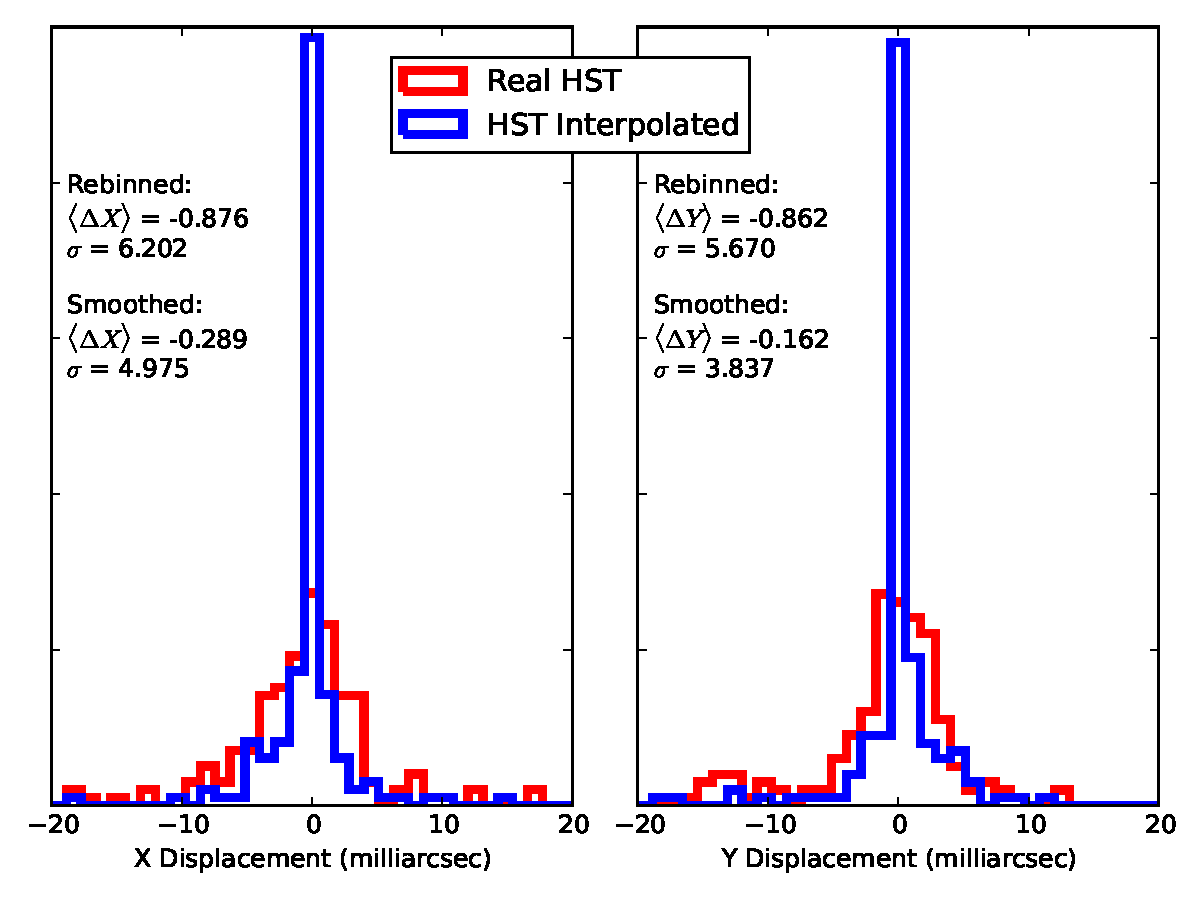
\includegraphics[width=.48\textwidth]{./figures_sls/imgpos_histogramrebinsmooth-eps-converted-to.pdf}
	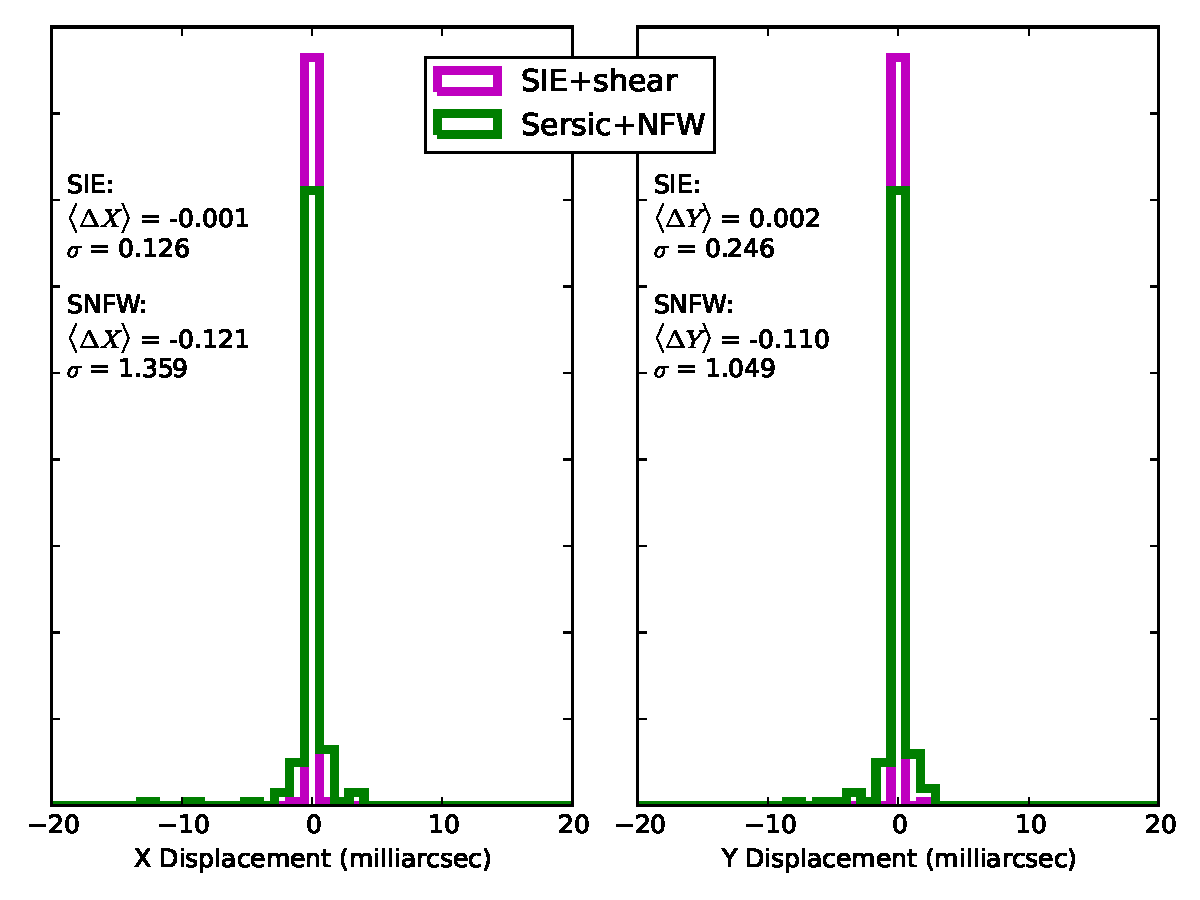
\includegraphics[width=.48\textwidth]{./figures_sls/imgpos_histogram-eps-converted-to.pdf}
	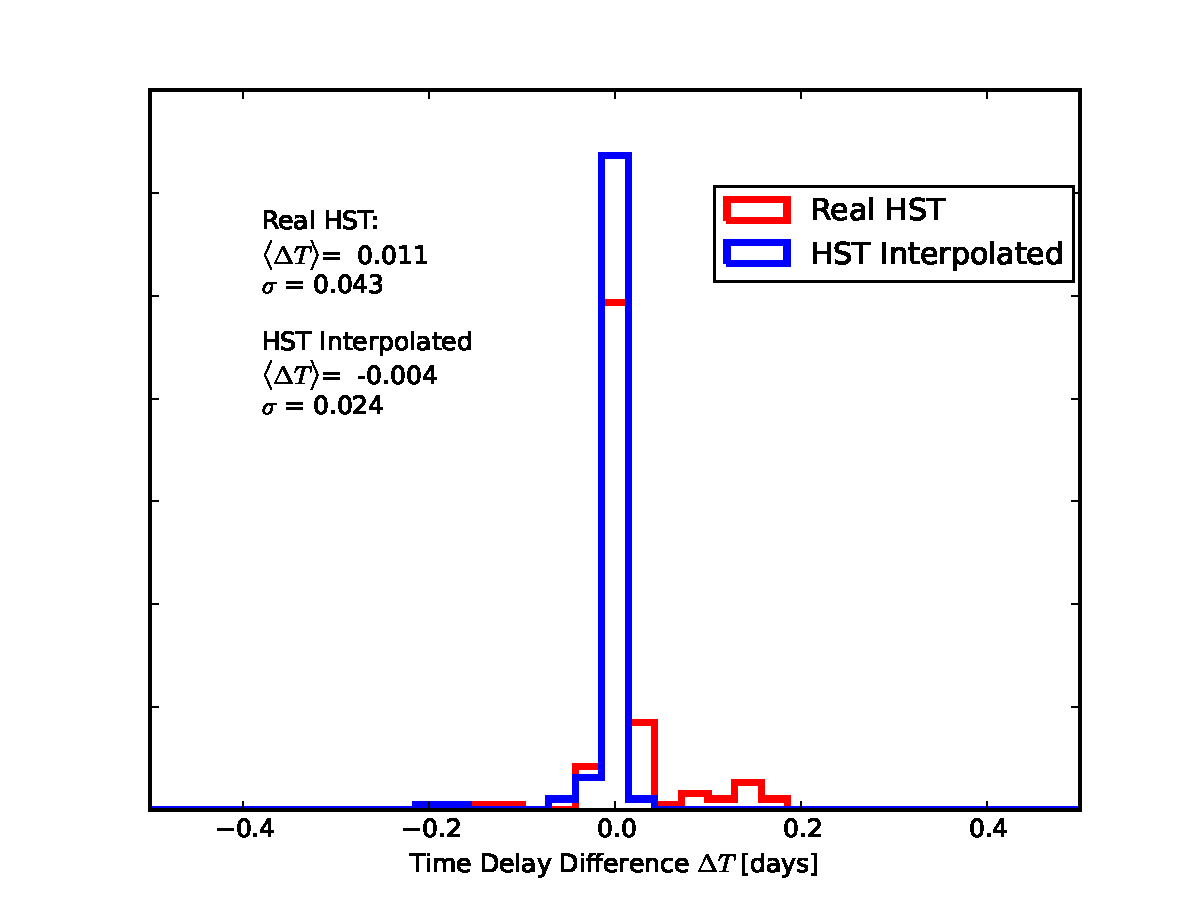
\includegraphics[clip,trim=1cm 0cm 1.5cm 1cm,width=.49\textwidth]{./figures_sls/tdel_histogramrebinsmooth-eps-converted-to.pdf}
	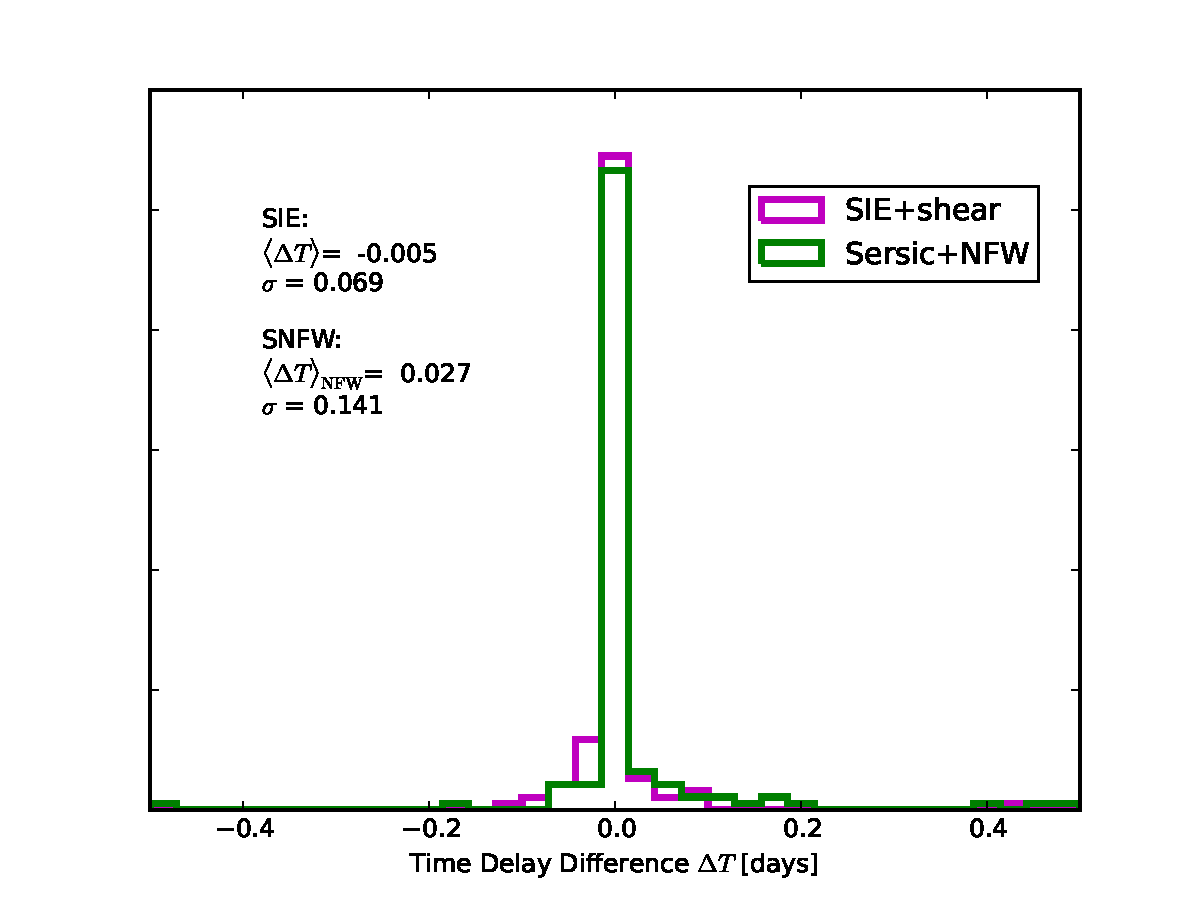
\includegraphics[clip,trim=1.5cm 0cm 1cm 1cm,width=.49\textwidth]{./figures_sls/tdelay_histogram-eps-converted-to.pdf}
	\caption[Astrometric and time delay residuals from the fits to mock lenses]{\label{fig:pos_tdel}Distributions of the difference in positions (top) and times delays (bottom) from the mean of the \textit{Truth} distributions. Standard deviation, denoted by $\sigma$ is displayed for each data set. The absence of measurement noise in our mock data results in the narrow distributions, whose width is determined by specific lensing properties of each model.}
\end{figure*}
\begin{figure*}
	\centering
	%\begin{tabular}{cc}
	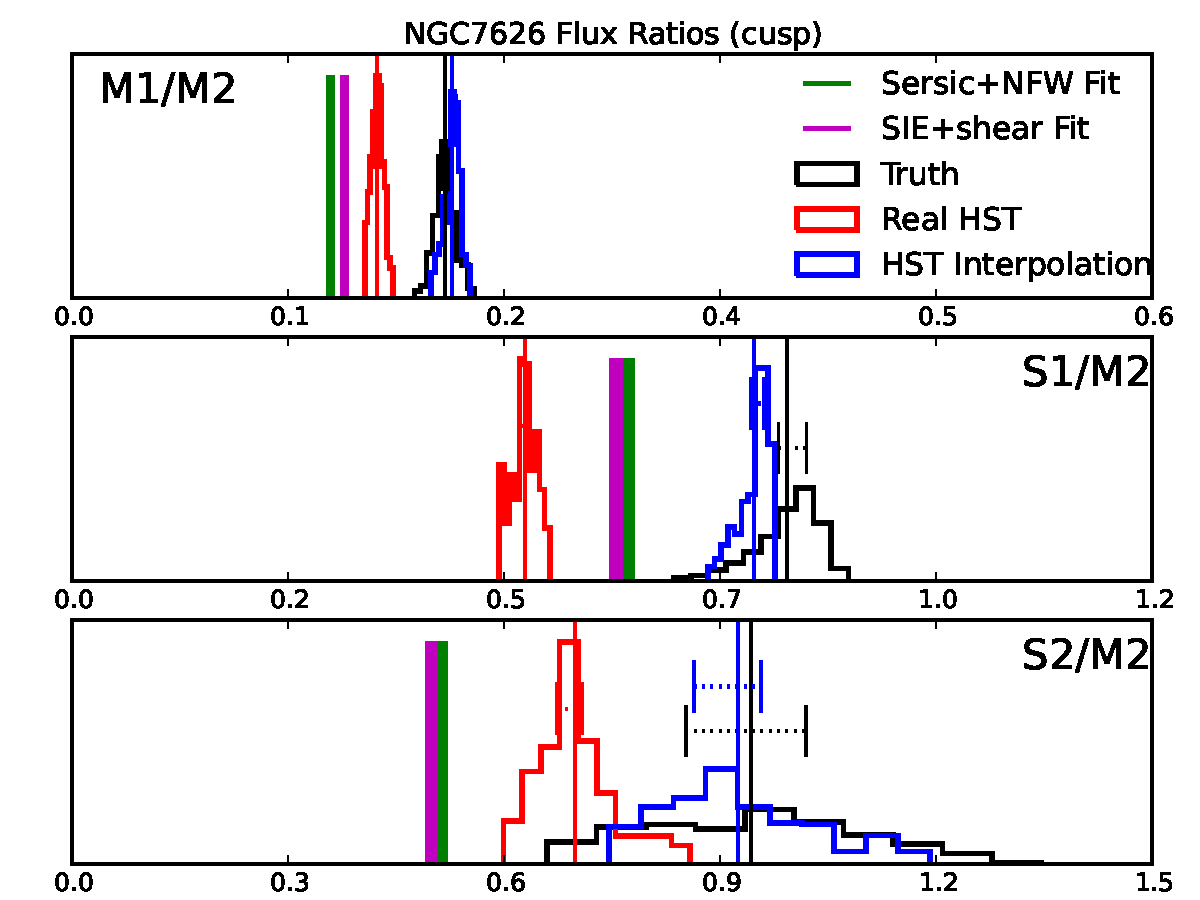
\includegraphics[clip,trim=.85cm 0cm .1cm
	0cm,width=0.48\linewidth,keepaspectratio]{./figures_sls/NGC7626_cusp_fluxratios-eps-converted-to.pdf}
	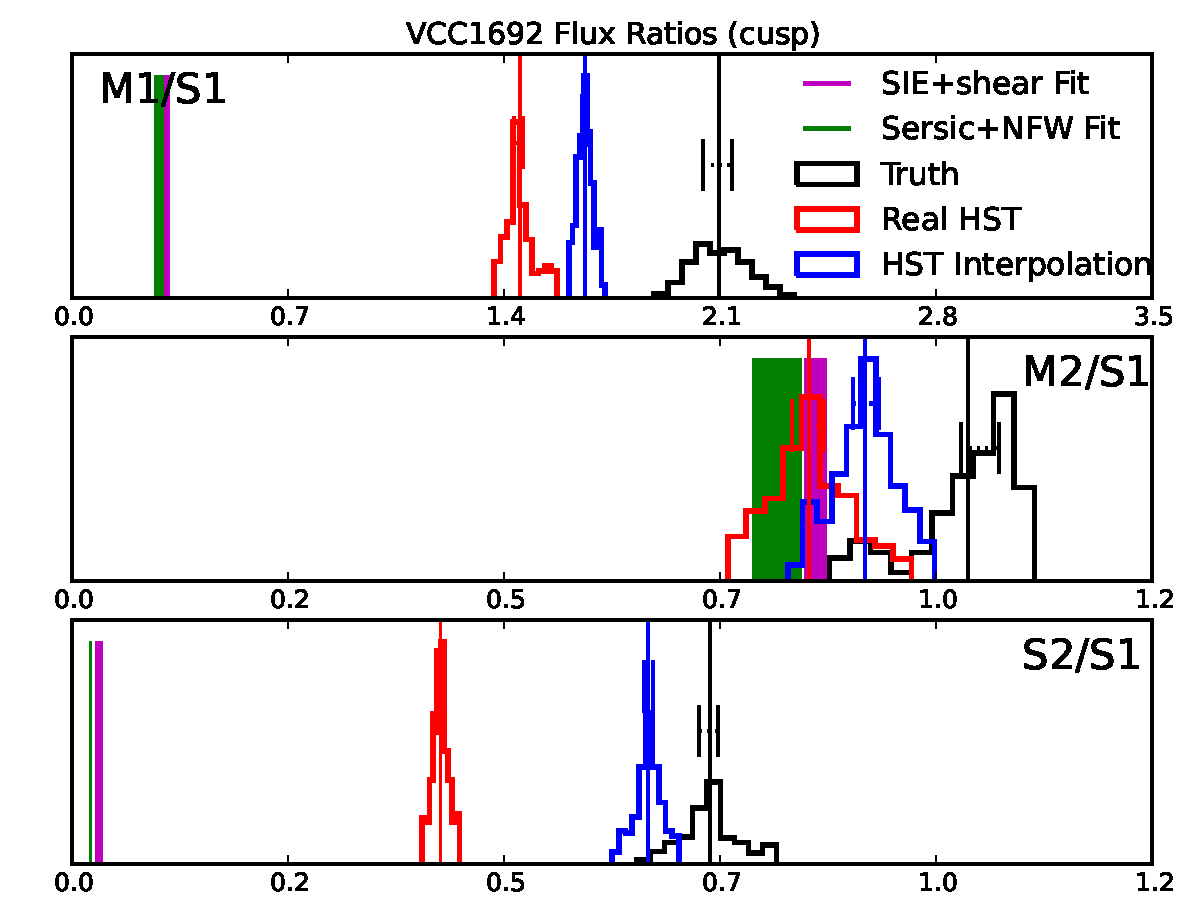
\includegraphics[clip,trim=.9cm 0cm .2cm
	0cm,width=0.48\linewidth,keepaspectratio]{./figures_sls/VCC1692_cusp_fluxratios-eps-converted-to.pdf}
	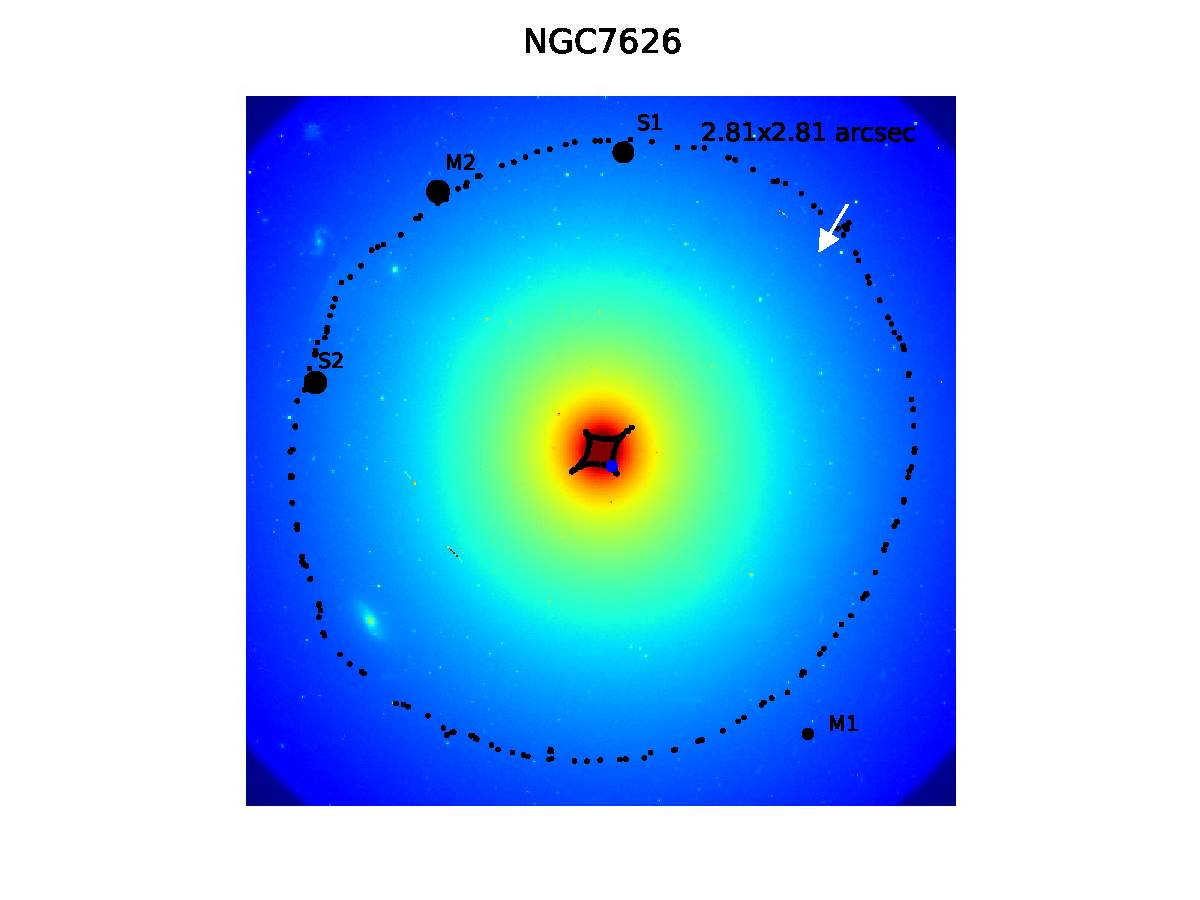
\includegraphics[trim=3cm 0cm 3cm 0cm,clip,width=.24\textwidth]{./figures_sls/kappamap_NGC7626_cusp_withshear-eps-converted-to.pdf}
	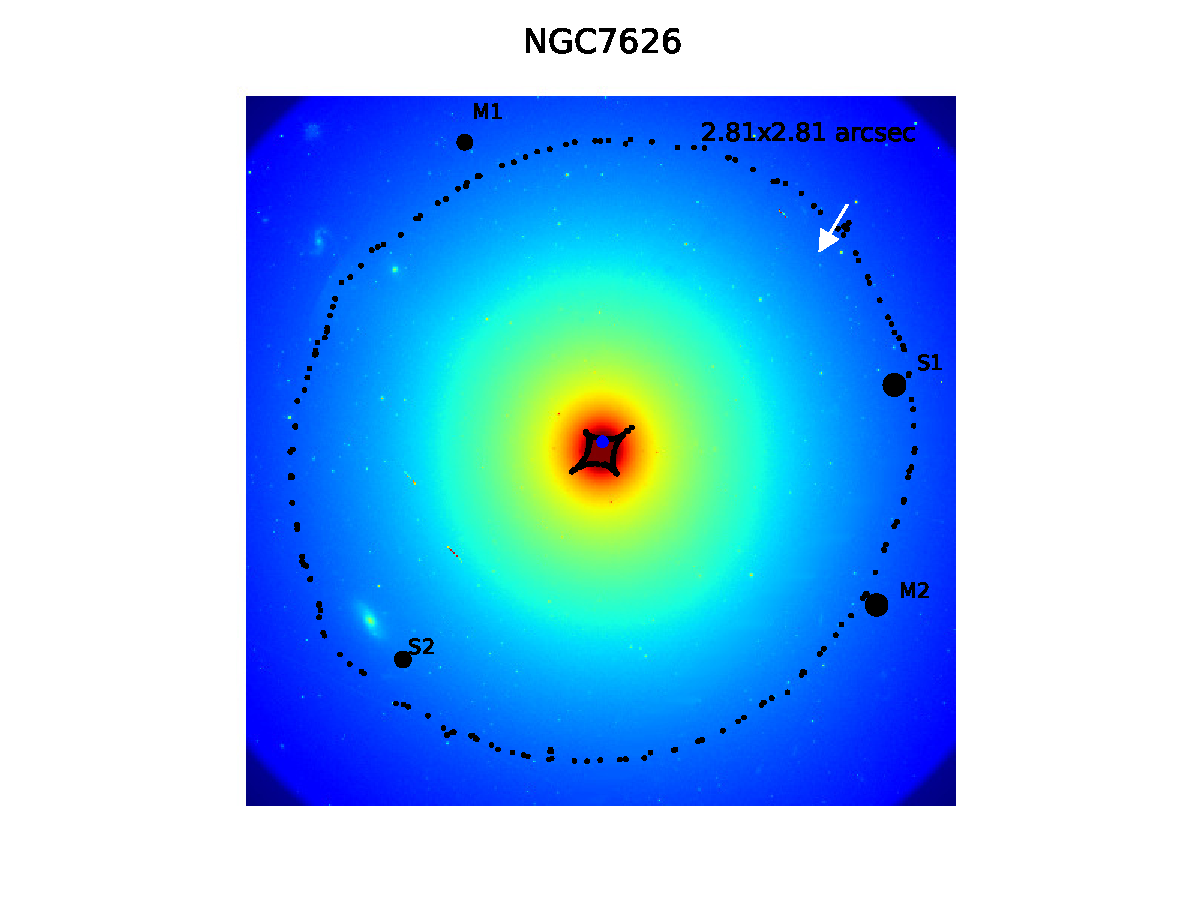
\includegraphics[trim=3cm 0cm 3cm 0cm,clip,width=.24\textwidth]{./figures_sls/kappamap_NGC7626_fold_withshear-eps-converted-to.pdf}
	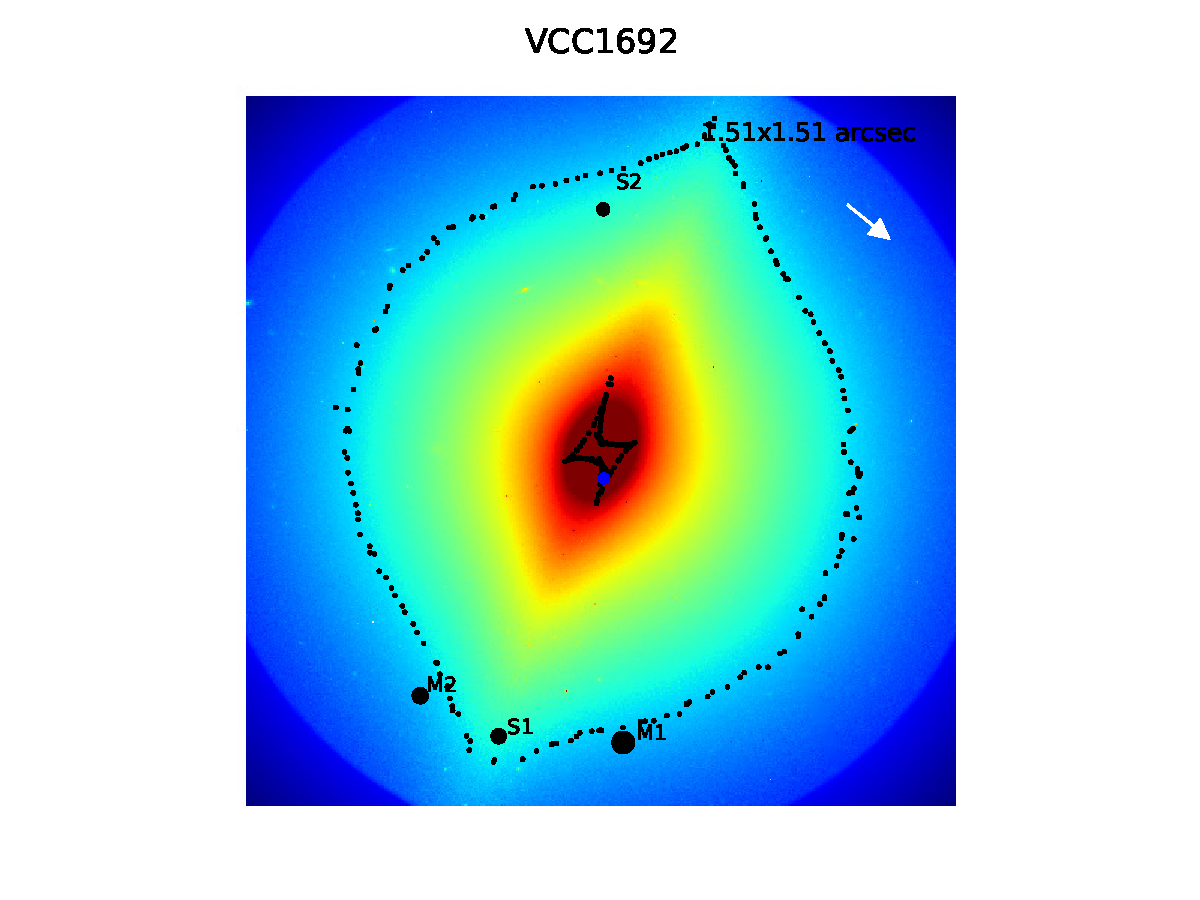
\includegraphics[trim=3cm 0cm 3cm 0cm,clip,width=.24\textwidth]{./figures_sls/kappamap_VCC1692_cusp_withshear-eps-converted-to.pdf}
	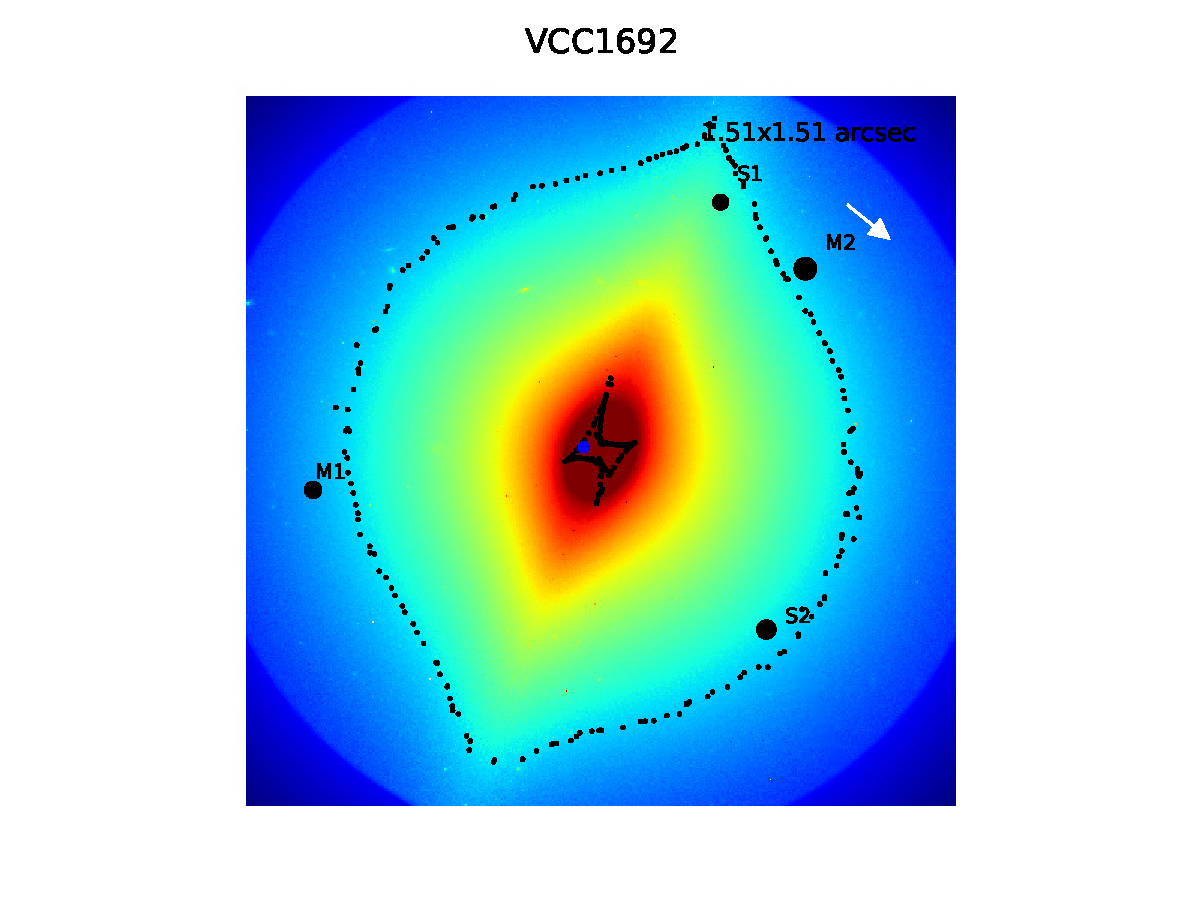
\includegraphics[trim=3cm 0cm 3cm 0cm,clip,width=.24\textwidth]{./figures_sls/kappamap_VCC1692_fold_withshear-eps-converted-to.pdf}
	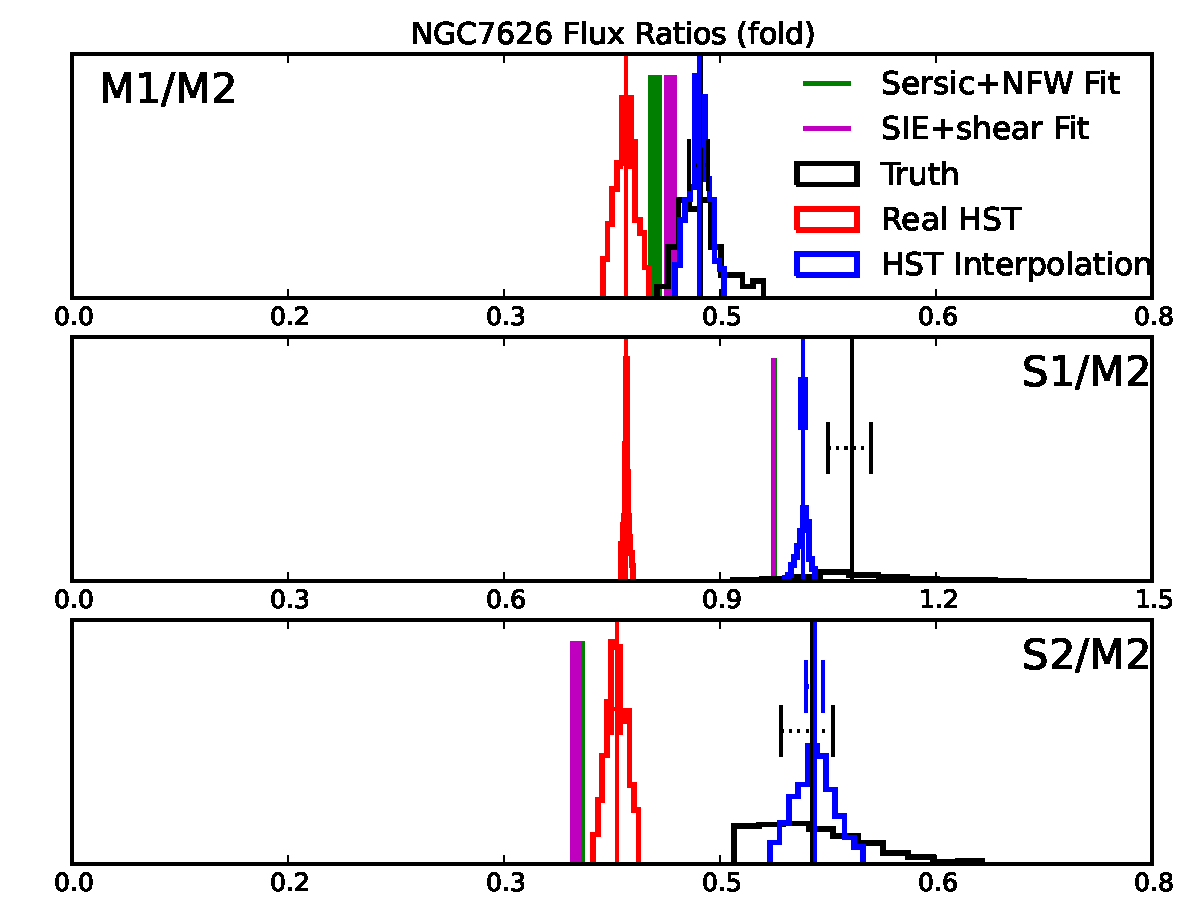
\includegraphics[clip,trim=.85cm 0cm .1cm
	0cm,width=0.48\linewidth,keepaspectratio]{./figures_sls/NGC7626_fold_fluxratios-eps-converted-to.pdf}
	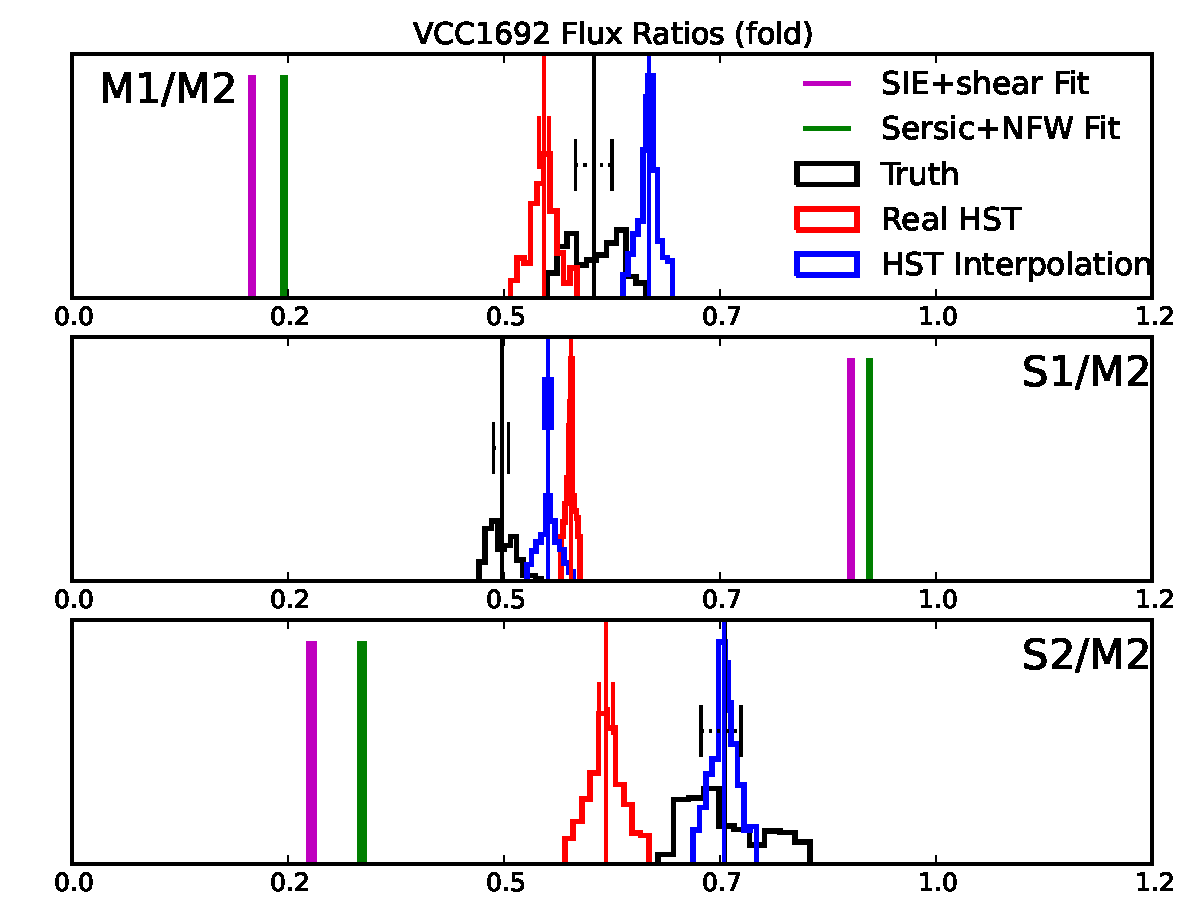
\includegraphics[clip,trim=.9cm 0cm .2cm
	0cm,width=0.48\linewidth,keepaspectratio]{./figures_sls/VCC1692_fold_fluxratios-eps-converted-to.pdf}
	\caption[Flux ratio pdfs and mass maps of VCC1692 and NGC7626]{\label{fig:fluxratios} Flux ratio distributions for two anomalous systems, NGC7626 and VCC1692. Images are classified as minima (M) or saddle points (S) of the time delay surface. The outer critical curve and astroid caustic are marked by black points, while the source position is marked as a blue point. The line in the upper right corner indicates the direction of the applied external shear. {\bf{\emph{Left}}}: The mock lens systems created from NGC7626 {\bf{\emph{Right}}}: The mock lens systems created from VCC1692 }.
\end{figure*}
\begin{figure*}
	\centering
	%\begin{tabular}{cc}
	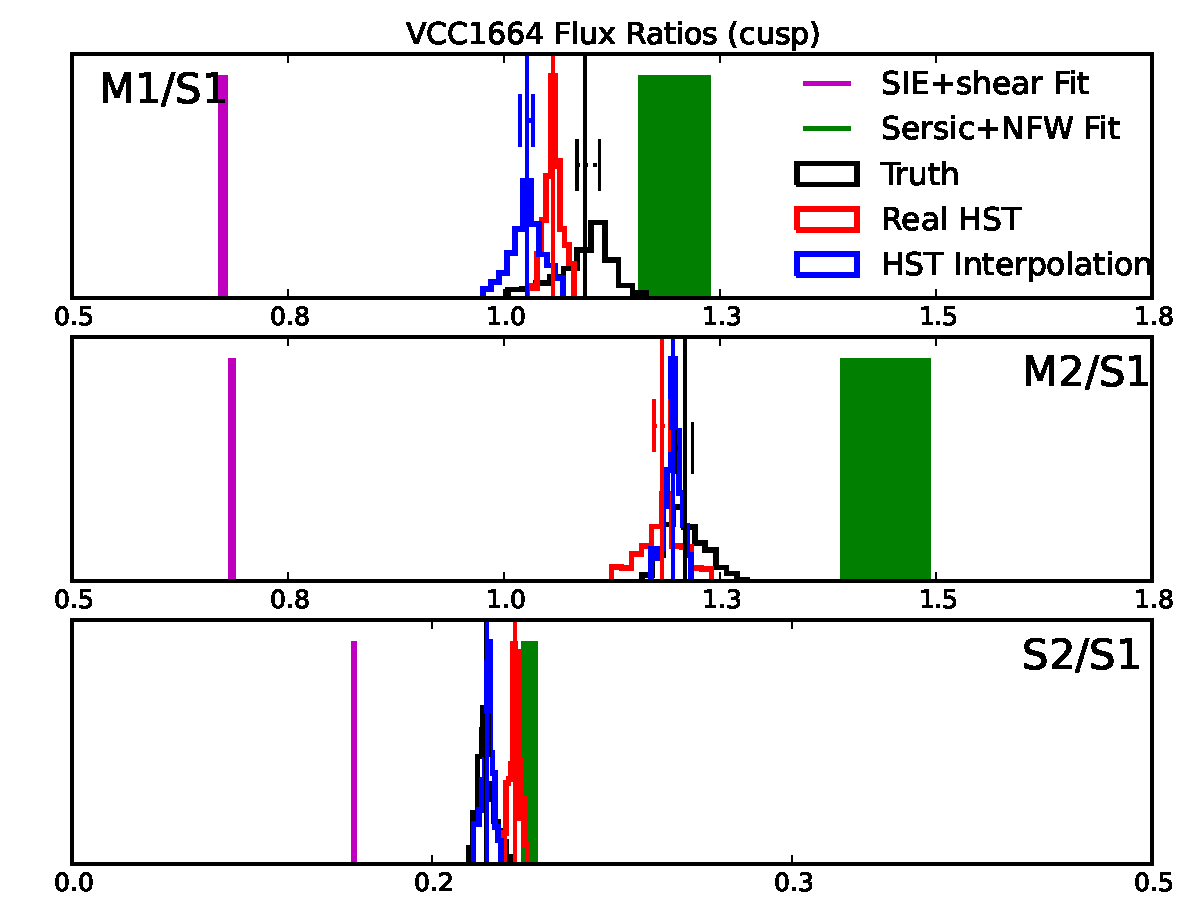
\includegraphics[clip,trim=.85cm 0cm .1cm
	0cm,width=0.48\linewidth,keepaspectratio]{./figures_sls/VCC1664_cusp_fluxratios-eps-converted-to.pdf}
	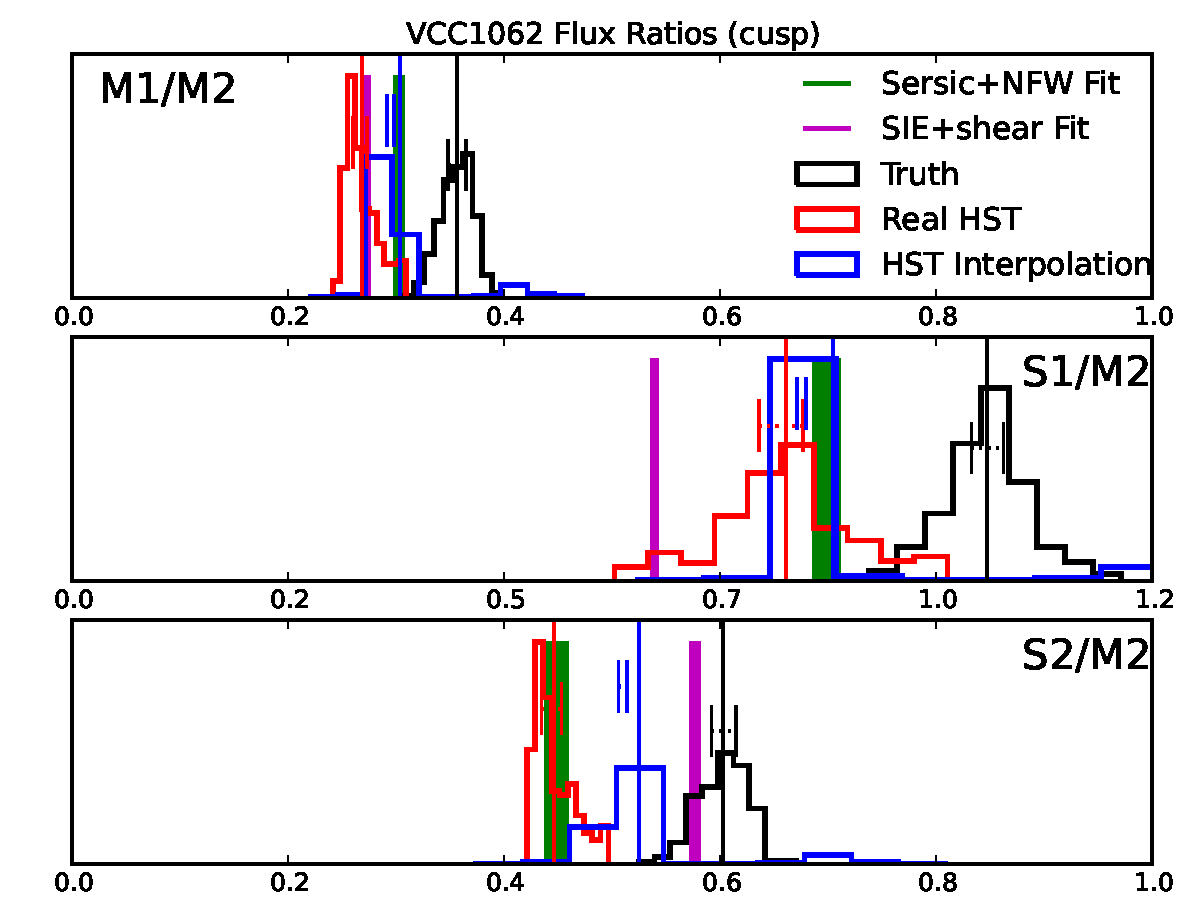
\includegraphics[clip,trim=.9cm 0cm .2cm
	0cm,width=0.48\linewidth,keepaspectratio]{./figures_sls/VCC1062_cusp_fluxratios-eps-converted-to.pdf}
	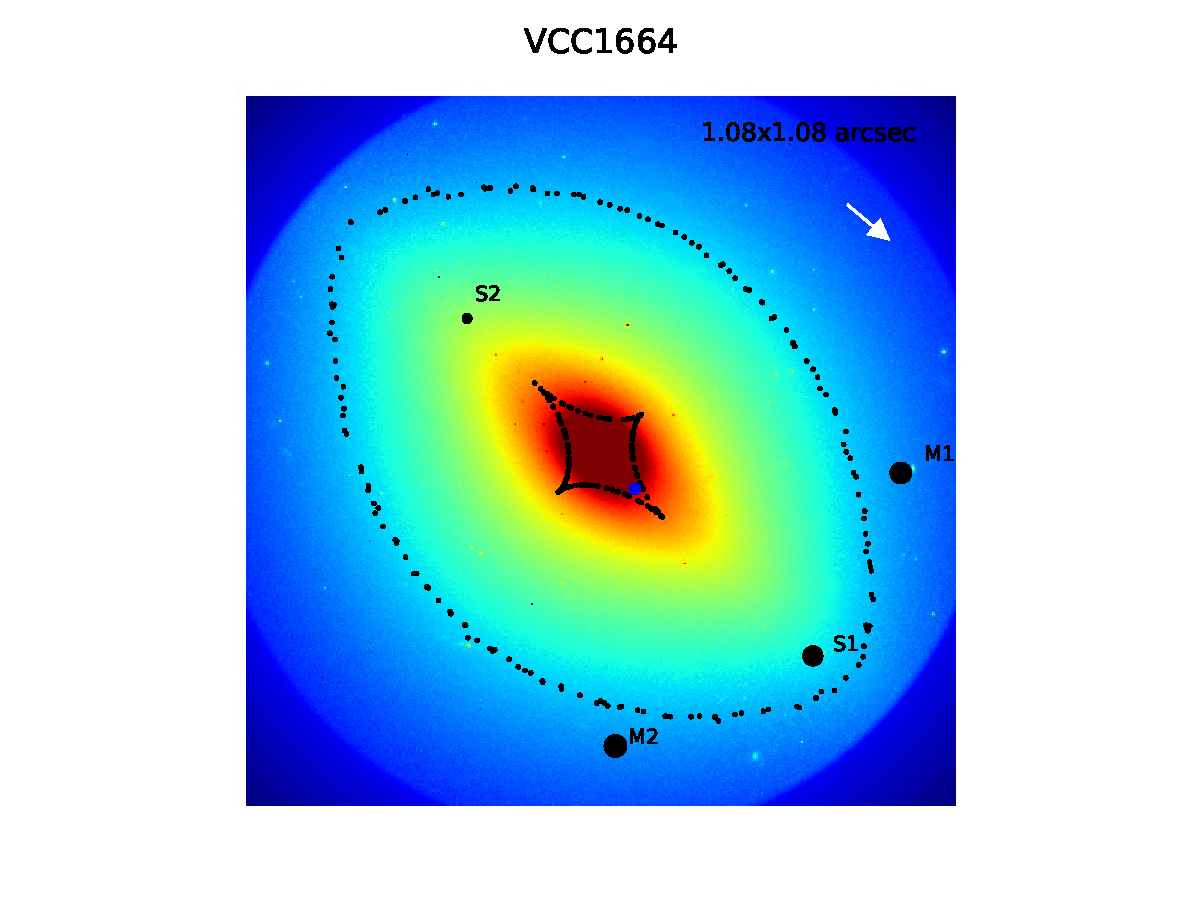
\includegraphics[trim=3cm 0cm 3cm 0cm,clip,width=.24\textwidth]{./figures_sls/kappamap_VCC1664_cusp_withshear-eps-converted-to.pdf}
	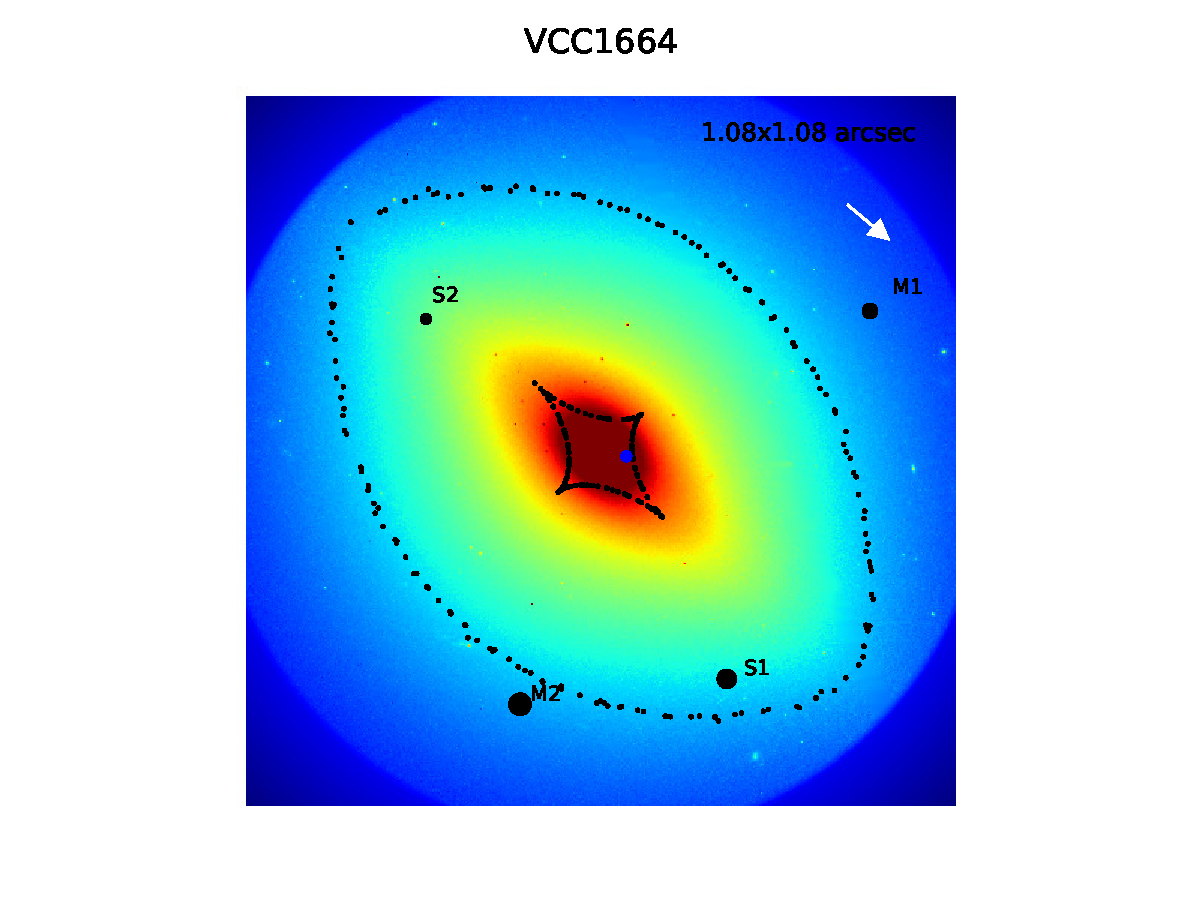
\includegraphics[trim=3cm 0cm 3cm 0cm,clip,width=.24\textwidth]{./figures_sls/kappamap_VCC1664_fold_withshear-eps-converted-to.pdf}
	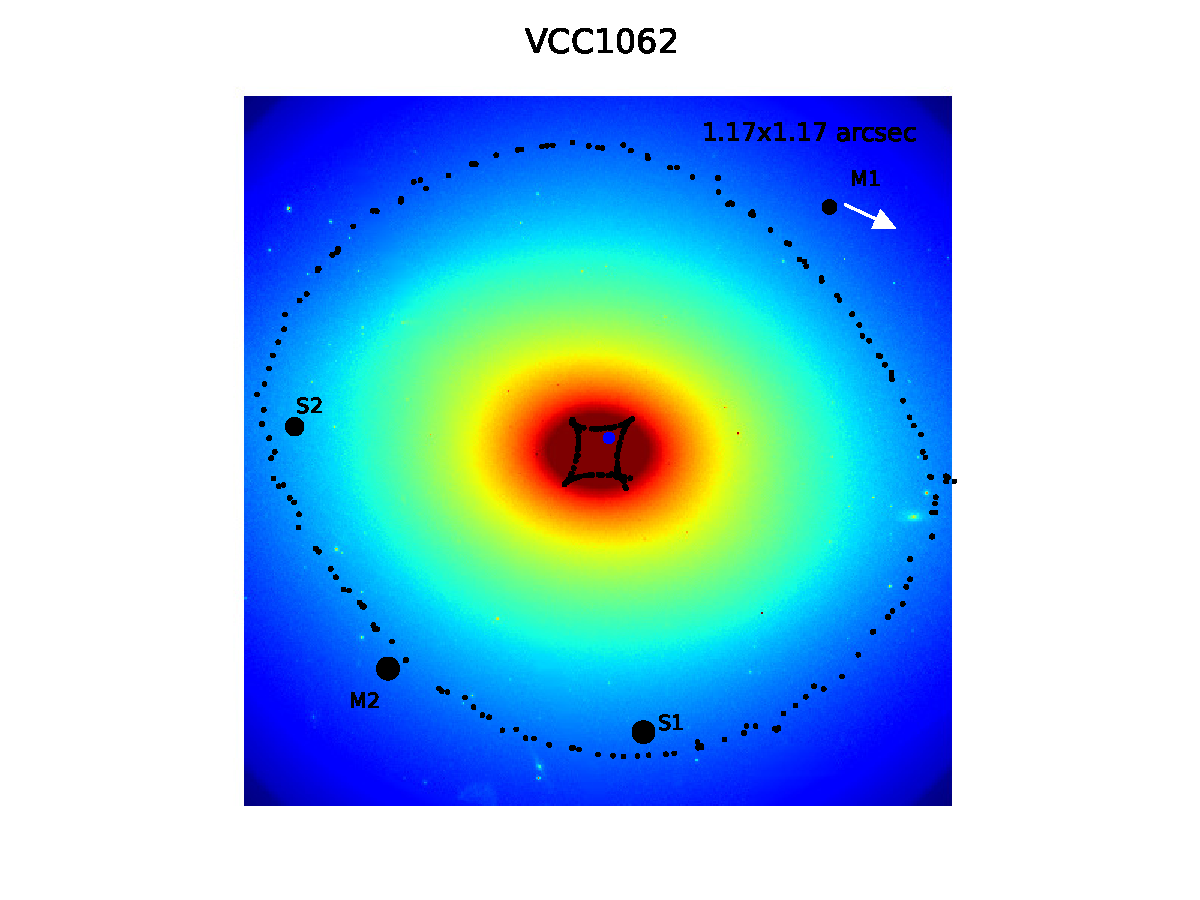
\includegraphics[trim=3cm 0cm 3cm 0cm,clip,width=.24\textwidth]{./figures_sls/kappamap_VCC1062_cusp_withshear-eps-converted-to.pdf}
	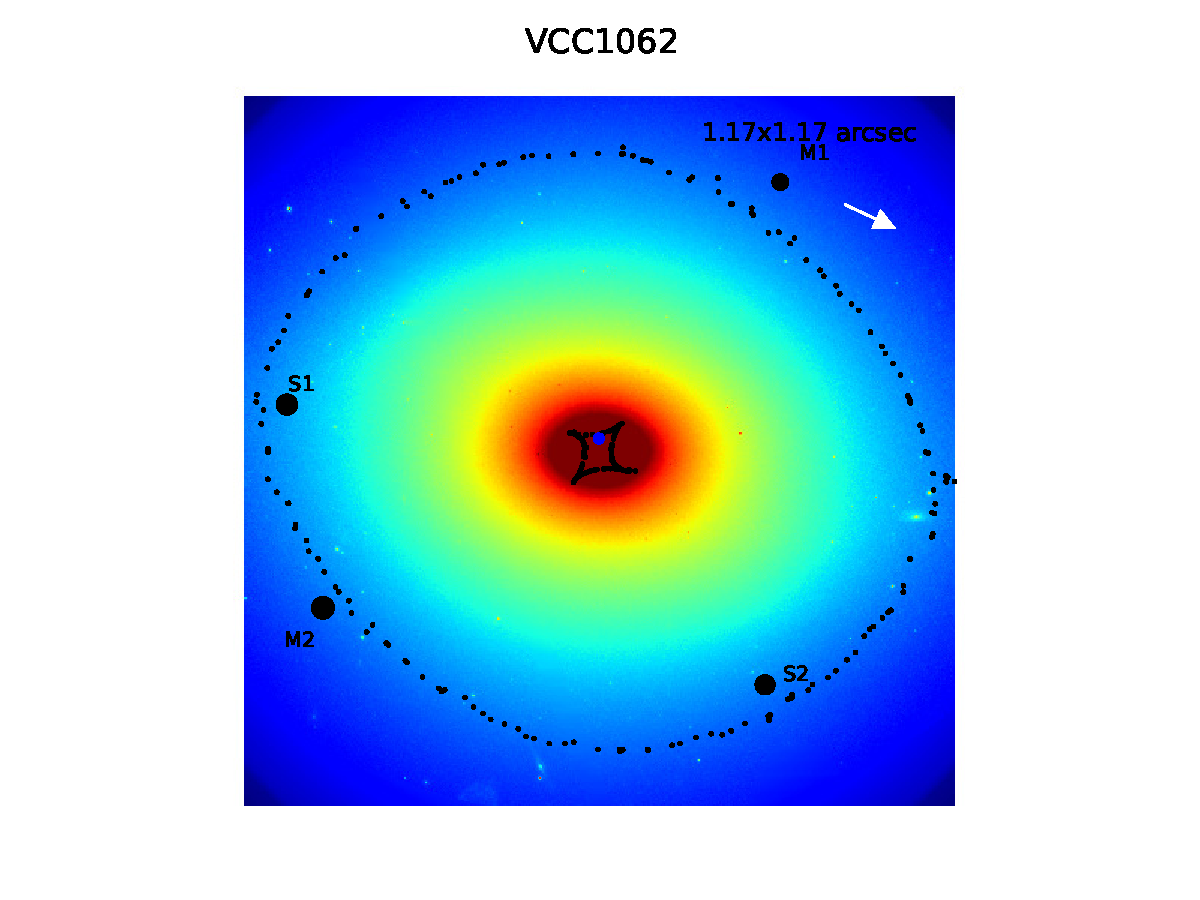
\includegraphics[trim=3cm 0cm 3cm 0cm,clip,width=.24\textwidth]{./figures_sls/kappamap_VCC1062_fold_withshear-eps-converted-to.pdf}
	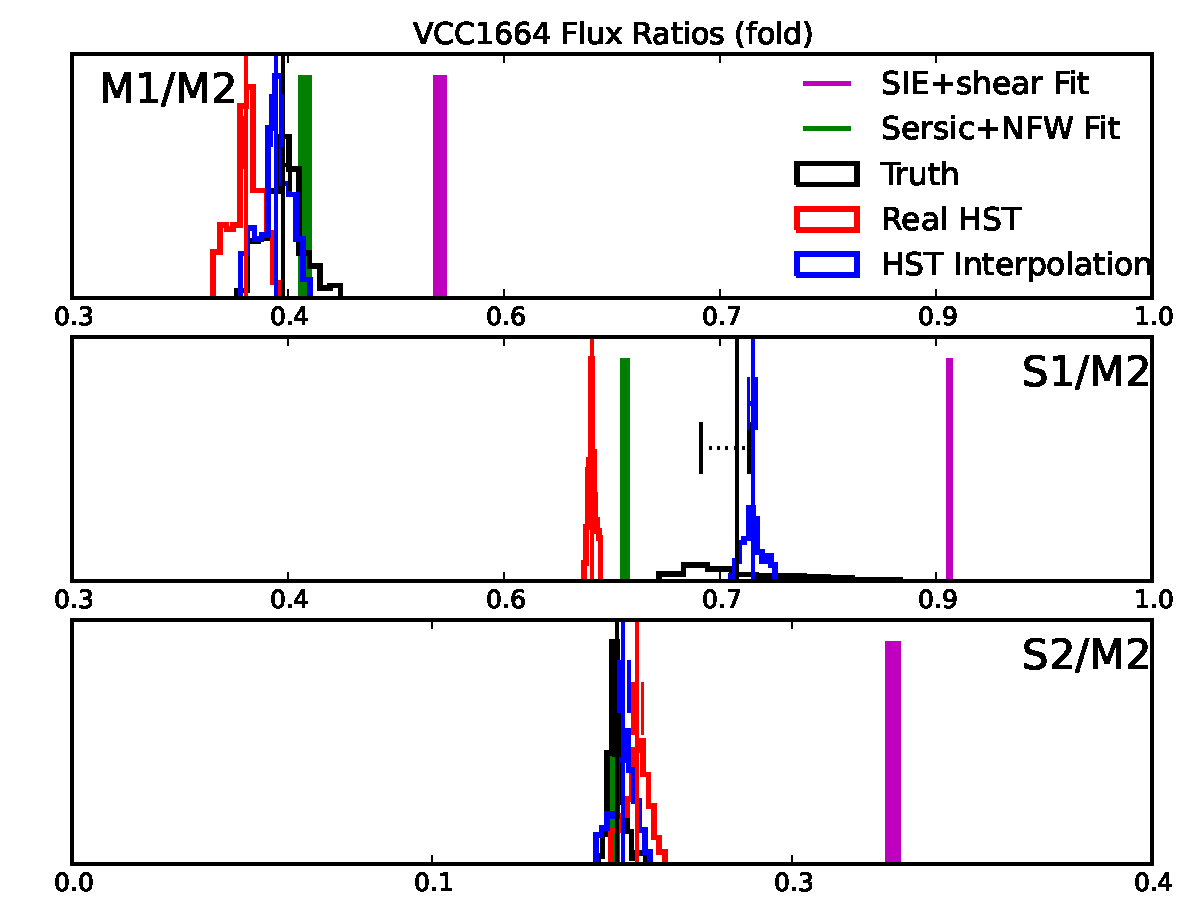
\includegraphics[clip,trim=.85cm 0cm .1cm
	0cm,width=0.48\linewidth,keepaspectratio]{./figures_sls/VCC1664_fold_fluxratios-eps-converted-to.pdf}
	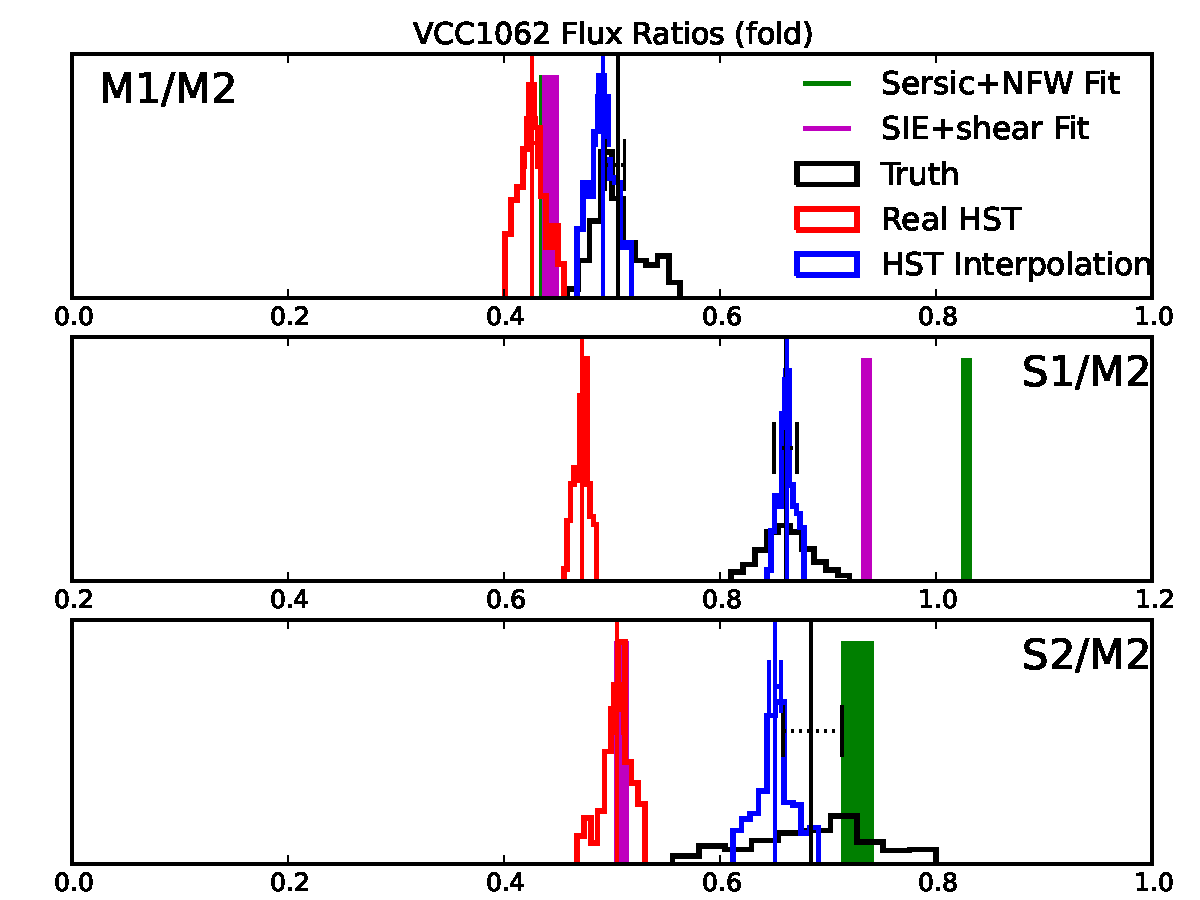
\includegraphics[clip,trim=.9cm 0cm .2cm
	0cm,width=0.48\linewidth,keepaspectratio]{./figures_sls/VCC1062_fold_fluxratios-eps-converted-to.pdf}
	\caption[Flux ratio pdfs and mass maps of VCC1664 and VCC1062]{\label{fig:fluxratios2} Flux ratio distributions for two anomalous systems, VCC1664 and VCC1692. Images are classified as minima (M) or saddle points (S) of the time delay surface. The outer critical curve and astroid caustic are marked by black points, while the source position is marked as a blue point. The line in the upper right corner indicates the direction of the applied external shear. {\bf{\emph{Left}}}: The mock lens systems created from VCC1062 {\bf{\emph{Right}}}: The mock lens systems created from VCC1692.} 
\end{figure*}
In contrast, when fitting with the SNFW, we attempt to fit the lens by holding the parameters of the S{\'e}rsic profile describing each galaxy fixed while varying the properties of the NFW halo. We obtain the S{\'e}rsic parameters either from literature (see the references in Table 1), or by measuring them ourselves using {\tt {galfit}}. Specifically, in the first iteration we vary only the normalization of the S{\'e}rsic profile, the normalization of the NFW halo, the scale radius of the NFW, and the external shear and position angle. 

In most cases, this approach fails to fit the positions and time delays with a reduced $\chi^2 < 2.5$, which we take to be the threshold acceptable $\chi^2$ fit. We choose this $\chi^2$ to permit individual astrometric and time delay $\chi^2$ values greater than 1, resulting in a conservative measure of the degree to which our smooth potentials can recover image positions and time delays. As we do not add measurement noise to our data, the SIE and SNFW frequently fit the data almost exactly, resulting in reduced $\chi^2$ much less than unity. After the first iteration of fitting, for the systems with unacceptable model fits, we allow the S{\'e}rsic index, ellipticity and position angle of the S{\'e}rsic to vary, and attempt to fit the lens again. If this approach fails, we vary the effective radius, ellipticity and position angle. 

The complications we encounter trying to fit lenses with a single S{\'e}rsic model suggests that, for the purpose of lens modeling, a more complicated lens model is required to fit the luminous matter of a lens, e.g. a bulge+disk of different ellipticity or two components at different position angles. On the other hand, the success of a simple SIE model suggests that this simple model is sufficient in most cases to caputure the lensing effects of baryonic matter. Interestingly, fold configurations required more flexible models (with varying S{\'e}rsic index, ellipticity, and position angle) than cusp configurations. Overall, we find that an SIE model absorbs the combined properties of stellar mass and dark matter as well as, or better than, the SNFW model. In Table~\ref{table:fitting_list} we summarize the parameters we allow to vary when fitting with the SIE and SNFW models, and the results of the fit for each galaxy in our sample.
\section{Results}
\label{sect:results}
In this section, we compare the data obtained for the \textit{Truth}, \textit{Real HST}, and \textit{HST Interpolated} mock lenses, and the two analytic models, the SIE and SNFW. First, in 3.1 we investigate the extent to which positions and time delays vary between the \textit{Truth} data set and the four comparison models. Section 3.2 reviews the $R_{\rm{cusp}}$ and $R_{\rm{fold}}$ statistics, and present the values for these statistics we obtain for the \textit{Truth} model, side by side with observed $R_{\rm{cusp}}$ and $R_{\rm{fold}}$ statistics from real strong lenses, and characterize baryonic flux ratio anomalies by their coupling to astrometric anomalies. In 3.3, we examine in detail each anomalous system to understand the source of flux ratio anomaly, making use of magnification maps derived from our convergence maps. Finally, in 3.4 we discuss the the degree to which the \textit{Real HST}, \textit{HST Interpolated}, SIE and SNFW models recover the flux ratios, $R_{\rm{cusp}}$ and $R_{\rm{fold}}$ values of the data of the \textit{Truth} model. 

\subsection{Image Positions and Time Delays}

Since time delays and image positions depend on the total
gravitational potential, and the gradient of the potential,
respectively, one can expect these data to be relatively insensitive
to small perturbations to the gravitational potential, whether by dark
subhalos or by baryonic features. Therefore, it is expected that the
rebinned and smoothed models will yield similar image positions and
time delays as the \textit{Truth} model, and that both the SIE
and SNFW models we fit to the \textit{Truth} will also
accurately recover these data.

Our results are consistent with these expectations. In Figure~\ref{fig:pos_tdel} we plot the distributions of offsets between
means of the \textit{Truth} model, the three models based on
the unfiltered data (Models 1,2,3), and the SIE and SNFW fits to the
\textit{Truth} model. The standard deviations in the
distributions of image positions are comparable to the 0.003 arcsecond
uncertainty we assume in our lens models, while the standard
deviations in the distributions of time delays is an order of
magnitude smaller than our assumed uncertainty. For the
\textit{Real HST} and \textit{HST Interpolated} models, this indicates that
the information lost in the process of rebinning pixels, or convolving
with the smoothing kernal, does not, in most cases, significantly impact the predicted image positions and arrival times. For the SIE and SNFW fits, these results confirm that the image positions and time delays of real lenses are consistent with those produced by a smooth lens model, as expected.

While these results were expected a priori, this should not undermine their significance. The agreement of astrometric data between the different models we consider implies that luminous matter is highly unlikely to result in astrometric anomalies. Conversely, many real lenses with flux ratio anomalies similar to those we observe in our mocks exhibit flux ratio anomalies accompanied by astrometric anomalies, suggesting an avenue by which a baryonic lensing signal may be distinguished from other sources of anomaly. We will revisit this point in detail later in this section.
\subsection{Flux ratios and the $R_{\rm{cusp}}$ and $R_{\rm{fold}}$ relations, \textit{Truth} model vs. real lens systems}
In order to quantify the flux ratio anomaly across the full ensemble
of mock lenses, we consider the differences in the mean of each
distribution (explicitly, each $F_{i}$ denotes the mean of a
distribution for an image generated from a lens described by model
$i$). The mean is marked as vertical bar in
Figures~\ref{fig:fluxratios} and \ref{fig:fluxratios2}. In this work we consider the relative flux ratio anomalies $\delta F_i$, with respect to the \textit{Truth} data:
\begin{figure*}
	\centering
	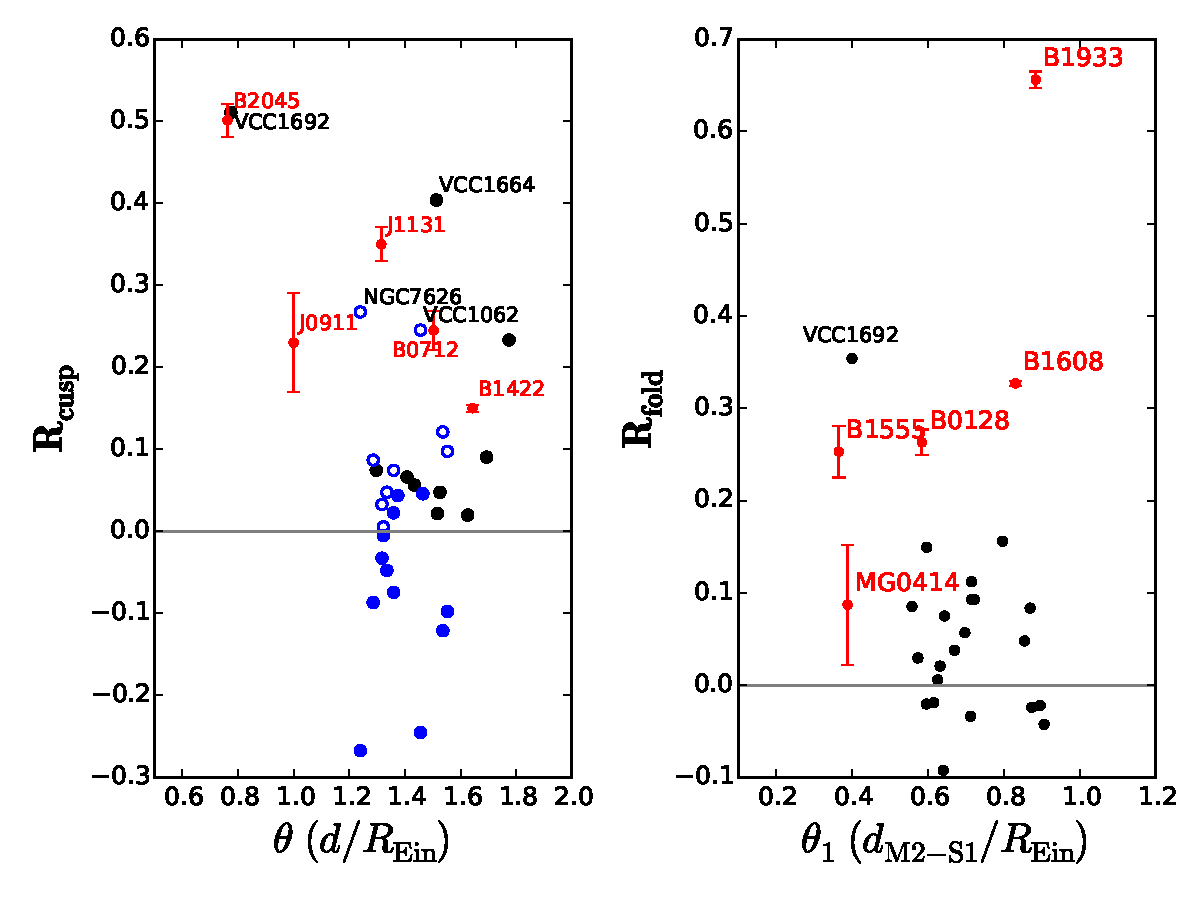
\includegraphics[trim=0cm 0cm 0cm 0cm,clip,width=.6\textwidth]{./figures_sls/dmax_vs_Rcuspfold-eps-converted-to.pdf}
	%\includegraphics[trim=5cm 1cm 6.5cm 2cm,clip,width=.15\textwidth]
	%{./figures_sls/cusptype_image-eps-converted-to.pdf}
	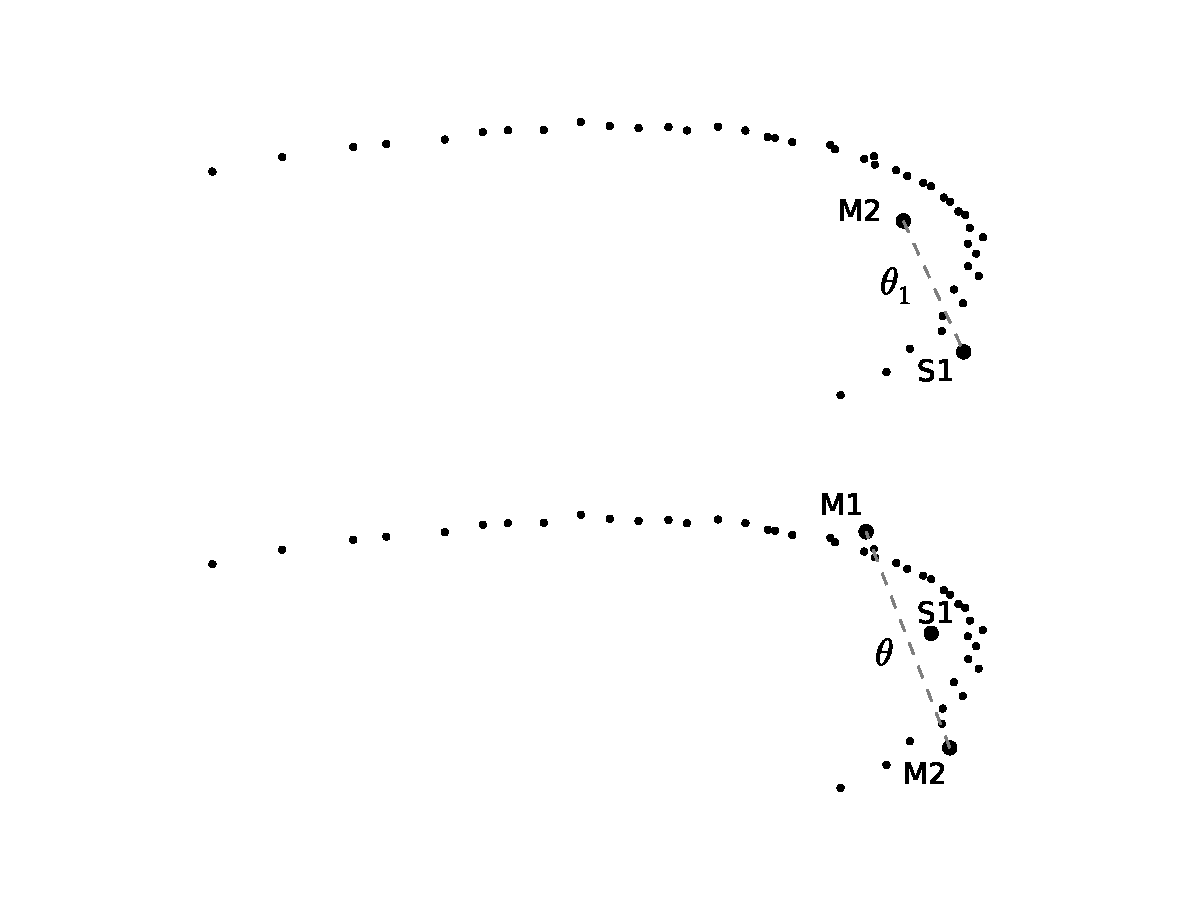
\includegraphics[trim=12cm 1cm 0cm 0.5cm,clip,width=.3\textwidth]{./figures_sls/fold_theta1.pdf}
	\caption[$R_{\rm{cusp}}$ and $R_{\rm{fold}}$ statistics of the \textit{Truth} models comapred with real lenses]{\label{fig:Rcuspfold_vs_real}$R_{\rm{cusp}}$ and $R_{\rm{fold}}$ statistics of the \textit{Truth} data (black), compared with a set of $R_{\rm{cusp}}$ and $R_{\rm{fold}}$ statistics of real lenses (red). An empty circle indicates the absolute value of an $R_{\rm{cusp}}$ that turns out to be negative. Fold (top) and cusp (bottom) image configurations,  with critical curves shown as small black dots and images labeled according to their classification as minima or saddle points. The distances between images $\theta_1$ and $\theta$, appearing in the left panels, are shown as dashed grey lines.}
\end{figure*}
\begin{equation}
\nonumber \delta F_i = \frac{| F_{Truth} - F_{model} |}{F_{Truth}}
\end{equation}

\noindent We calculate the commonly used $R_{\rm{cusp}}$ and $R_{\rm{fold}}$ statistics given by
%
\begin{eqnarray} \label{eq:rcuspfold1}
R_{cusp} &=& \dfrac{M_{1} + M_{2} - S_{1}}{M_{1} + M_{2} + S_{1}} \quad \rm{(major \ axis)} \\ \nonumber &=& \dfrac{M_2 - S_{1} - S_{2}}{M_{2} + S_{1} + S_{2}} \quad \rm{(minor \ axis)} \\\label{eq:rcuspfold2}R_{fold} &=& \frac{M_{2} - S_{1}}{M_{2} + S_{1}}
\end{eqnarray}
for each model. Major axis and minor axis cusps are defined by whether the central cusp image is the first saddle S1 (major) or the second minimum M2 (minor). The different configurations are shown on the right hand side of Figure~\ref{fig:Rcuspfold_vs_real}. It has been shown \cite{Schechter++02,Keeton03b} that small, compact deflectors in the lensing galaxy, or local perturbations, tend to suppress the brightness of images appearing on saddle points of the time delay surface, while preferentially magnifying minima. On the other hand, perturbations to the gravitational potential on scales larger than the image separation, or global perturbations, do not discriminate between minima and saddle points. The different responses of these cusp configurations to lens structures suggest they could potentially be used to differentiate between different sources of flux ratio anomalies.

For models 2-5, we compute the offset between the unsigned $R_{\rm{cusp}}$ and $R_{\rm{fold}}$ statistics
\begin{equation}
\nonumber \Delta R_{model} = ||R_{Truth}|- |R_{model}|| 
\end{equation}
Smooth lens models will yield values close to zero in the limit of vanishing distance between neighboring images, with small variations depending on the image separation and properties of the main lens model \cite{Keeton03,Keeton05}. Large values of $R_{\rm{cusp}}$ and $R_{\rm{fold}}$ are typically associated with perturbations to the lens potential on scales smaller than the image separation, and as such, these statistics are often used as a indicators of small scale structure near a lensed image.

\subsubsection{Distribution of $R_{\rm{cusp}}$ and $R_{\rm{fold}}$ for target galaxies}
In Figure \ref{fig:Rcuspfold_dis}, we plot the distributions of the $R_{\rm{cusp}}$ and $R_{\rm{fold}}$ statistics of the \textit{Truth} data for each of our target galaxies as a function of the largest distance (normalized by $R_{\rm{Ein}}$) between the three merging images $\theta$ (cusp lenses) or the merging pair $\theta_1$(fold lenses). Our sample of mock lenses contains $R_{\rm{cusp}}$ and $R_{\rm{fold}}$ statistics as high as 0.5 for cusp lenses, and as high as 0.35 for fold lenses.

In Figure \ref{fig:Rcuspfold_vs_real}, we plot the $R_{\rm{cusp}}$ values of ten real lenses, with data as reported in \cite{Keeton03} and \cite{Xu++15}. Several of these lenses, notably B2045 and B1933 have $R_{\rm{cusp}}$ and $R_{\rm{fold}}$ that are inconsistent with lensing by a smooth potential \cite{Keeton03}. \cite{Xu++15} showed some of these anomalies could be accounted for by introducing a population of dark subhalos and multipole potential terms in smooth lens models, but noted that the observed anomalies were unlikely to caused entirely by dark subhalos. 
\begin{figure}
	\centering
	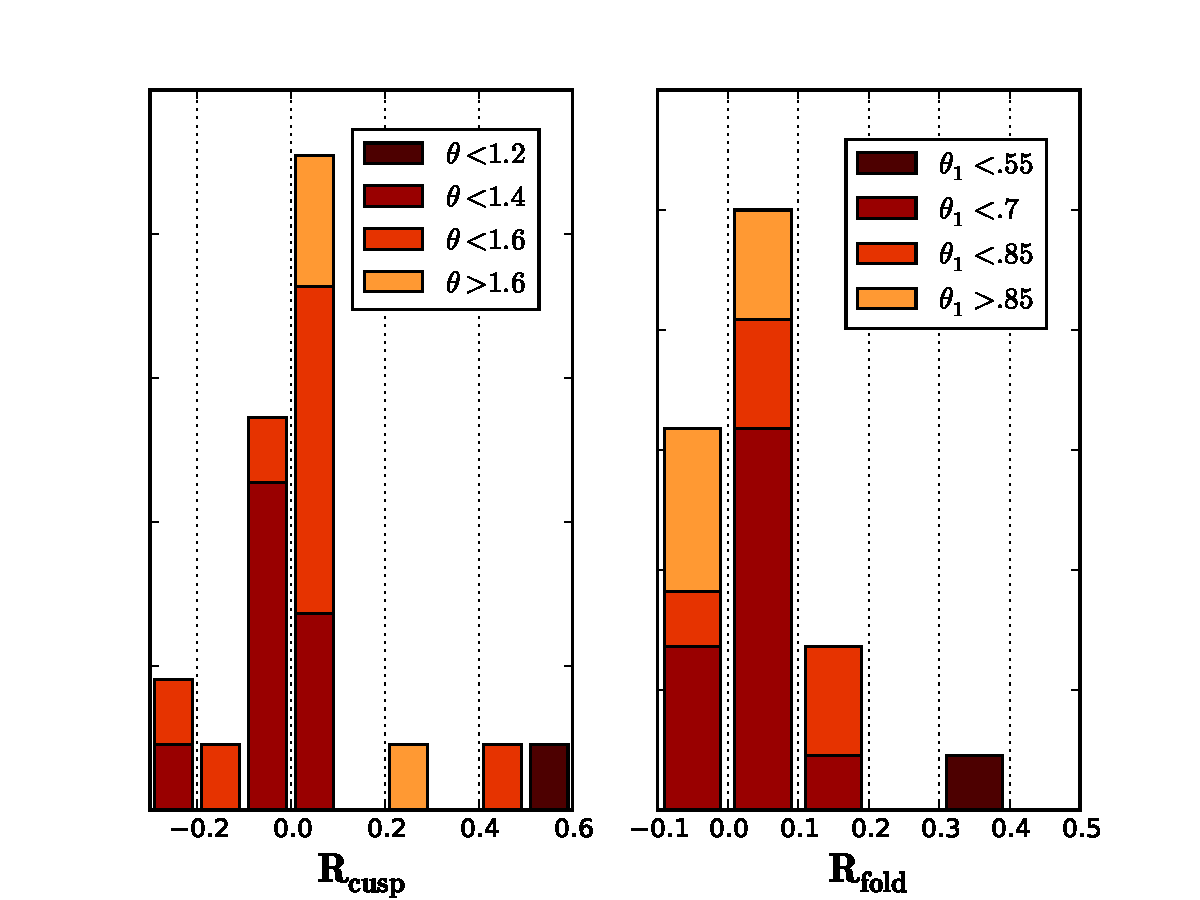
\includegraphics[trim=0cm 0cm 0cm 0cm,clip,width=.75\textwidth]{./figures_sls/Rcuspfold_dis-eps-converted-to.pdf}
	\caption[$R_{cusp}$ and $R_{\rm{fold}}$ distributions of the \textit{Truth} model]{\label{fig:Rcuspfold_dis}Distributions of $R_{cusp}$ and $R_{\rm{fold}}$ statistics of the \textit{Truth} data, color coded by the largest separation between the three merging images $\theta$ (for cusp configurations) or the separation between the merging image pair $\theta_1$ (for fold configurations), normalized by the Einstein radius.} 
\end{figure}
\begin{figure}
	\centering
	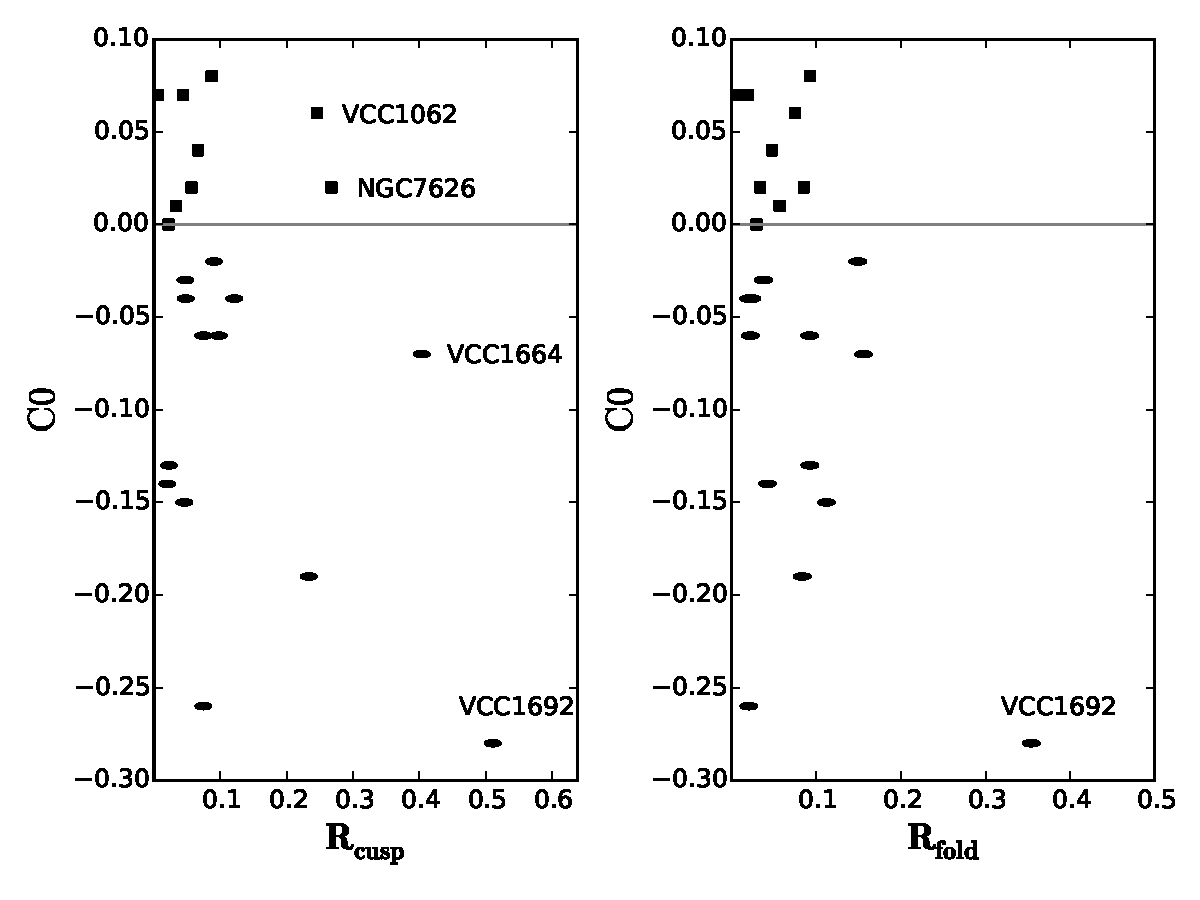
\includegraphics[trim=0cm 0cm 0cm .4cm,clip,width=.75\textwidth]{./figures_sls/C0_vs_Rcuspfold_truth-eps-converted-to.pdf}
	\caption[Disyness and boxyness of mock lenses]{\label{fig:C0_vs_Rcuspfold} Diskyness and boxyness for each mock deflector, described by the {\tt {galfit} }parameter $C0$. A positive $C0$ corresponds to boxy isophotes, while a negative value indicates diskyness. The anomalous systems shown in Figures \ref{fig:fluxratios}, \ref{fig:fluxratios2}, and \ref{fig:Rcuspfold_vs_real} are labeled.}
\end{figure}
In the following paragraphs, we will focus attention on the 4 systems with large $R_{\rm{cusp}}$ and $R_{\rm{fold}}$ anomalies in order to understand their origin, and to gain insight into how a baryon-induced induced flux ratio anomaly might reveal itself in an observational scenario.While we juxtapose real lens systems with our mock lenses in Figure~\ref{fig:Rcuspfold_vs_real}, we do not argue that baryons are responsible for the anomalies seen in these systems. Rather, we emphasize that features of the luminous matter in a lensing galaxy can give rise to the large values of $R_{\rm{cusp}}$ and $R_{\rm{fold}}$ typically associated with non-baryonic substructure - albeit rarely - especially in systems with a stellar disk or other irregularities. The stellar mass components and flux ratio distributions for these lenses are shown in Figures \ref{fig:fluxratios} and \ref{fig:fluxratios2}, while maps of the magnification surfaces are shown in Figures \ref{fig:magmaps_VCC1692c}, \ref{fig:magmaps_VCC1664}, \ref{fig:magmaps_NGC7626}, \ref{fig:magmaps_VCC1062}, and \ref{fig:magmaps_VCC1692f}.
Unsurprisingly, three of the most anomalous mock lenses show evidence for disky or boxy isophotes (see Figure \ref{fig:C0_vs_Rcuspfold}). The remaining system, NGC7626, has an $R_{\rm{cusp}}$ anomaly that can can be partially accounted for by the presence of a background galaxy and globular clusters near the images. Three out of of four anomalous mock lenses have velocity dispersion below 200 km s$^{-1}$, unlike the high central velocity dispersion deflectors most likely to act as strong lenses. In light of the inflated percentage of low stellar velocity dispersion targets in our lens sample, which are more likely to contain disks and irregular morphological features than high velocity dispersion deflectors, the non-detection of flux ratio anomalies through most of our lens sample illustrates the sub-dominant nature of flux ratio anomalies caused by luminous matter. 
\subsection{Analysis of Anomalous Systems}
Analyzing the few mock deflectors where the luminous matter of the lensing galaxy influences the flux ratios serves to illustrate how stellar mass can affect lensing observables. We will first inspect the cusp configurations, followed by the fold configurations.
\subsubsection{Cusps}
\begin{itemize}
	\begin{figure*}
		\centering
		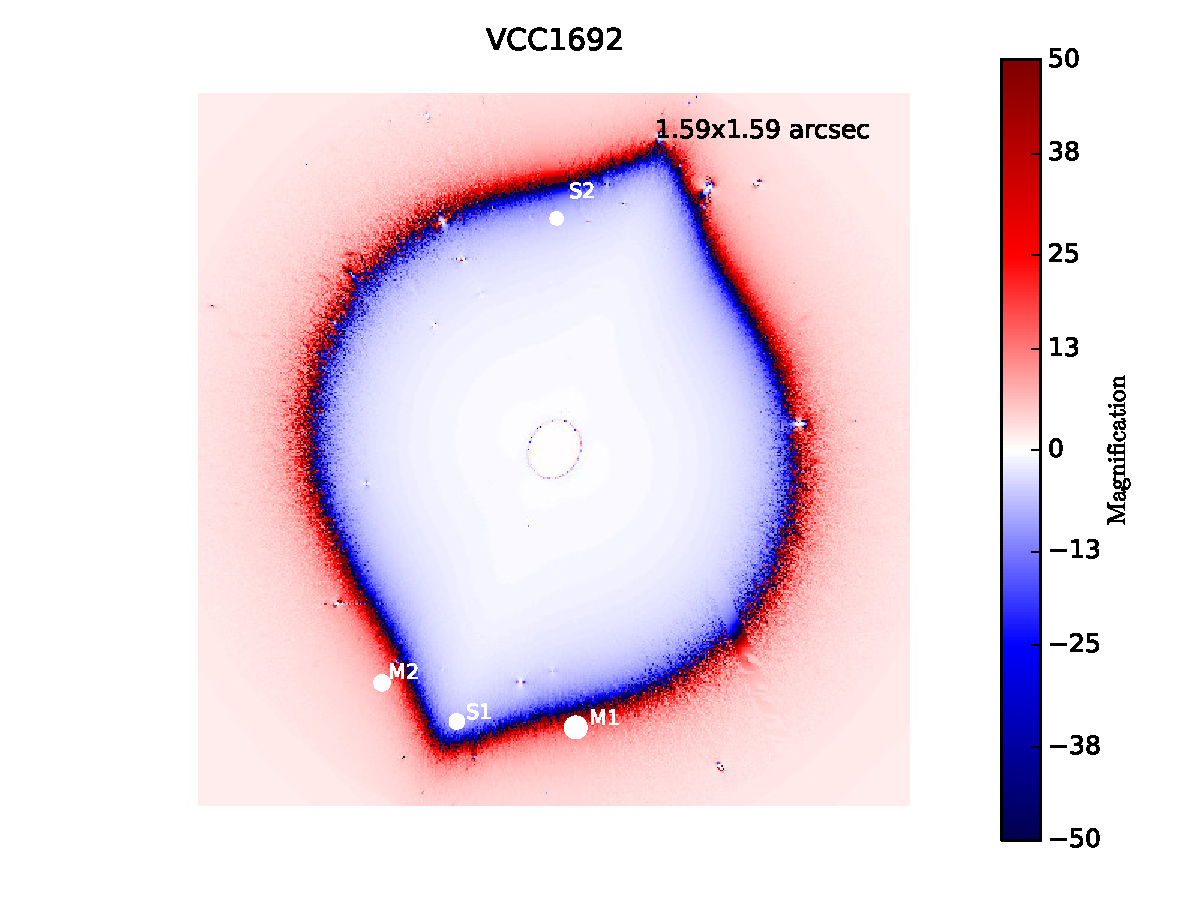
\includegraphics[clip,trim=2.5cm .5cm 1cm
		.25cm,width=.48\textwidth]{./figures_sls/magmap_VCC1692_cusp_withshear-eps-converted-to.pdf}
		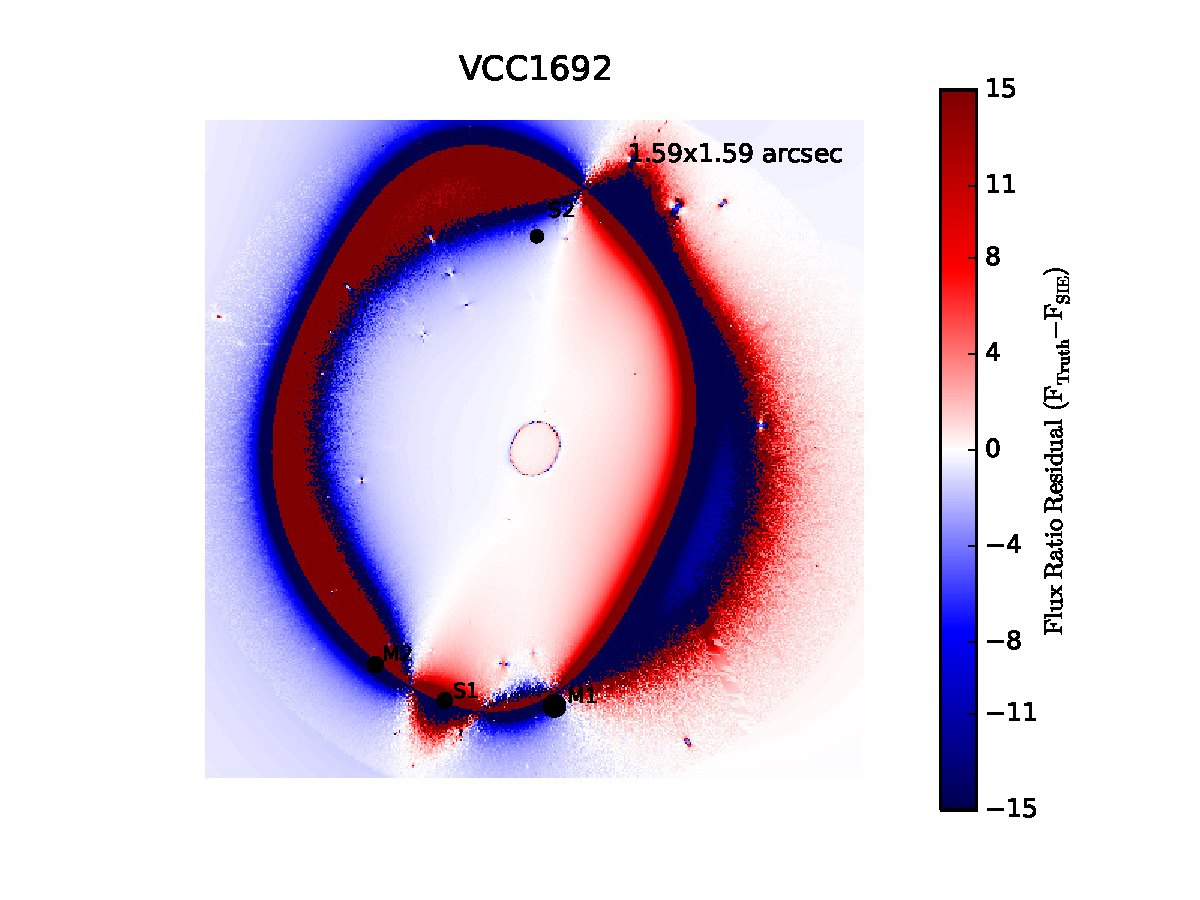
\includegraphics[clip,trim=2.5cm .5cm 1cm
		.25cm,width=.48\textwidth]{./figures_sls/res_map_VCC1692_cusp_withshear-eps-converted-to.pdf}
		\caption[Map of magnification residuals for mock lens VCC1692]{\label{fig:magmaps_VCC1692c} $R_{\rm{cusp}}$ anomaly. Left: Magnification surface derived from the convergence map. Right: Residuals after subtracting the magnification mag of the best fit SIE model. The interplay of the disk and external shear, which is nearly orthogonal to the disk position angle in this system, creates large residuals in the magnification surface that create a strong flux ratio anomaly.}
	\end{figure*}
	\begin{figure*} 
	\centering
		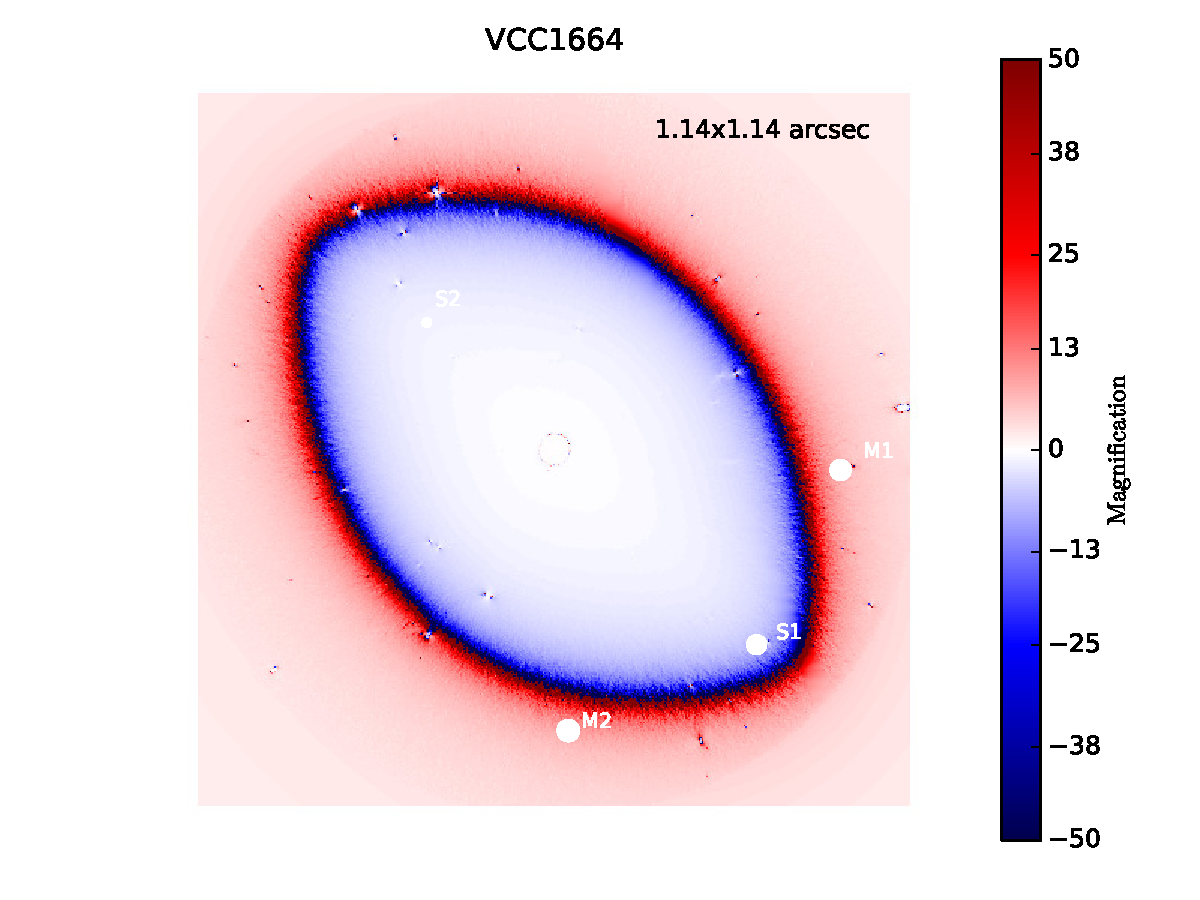
\includegraphics[clip,trim=2.5cm .5cm 1cm
		.25cm,width=0.48\linewidth,keepaspectratio]{./figures_sls/magmap_VCC1664_cusp_withshear-eps-converted-to.pdf}
		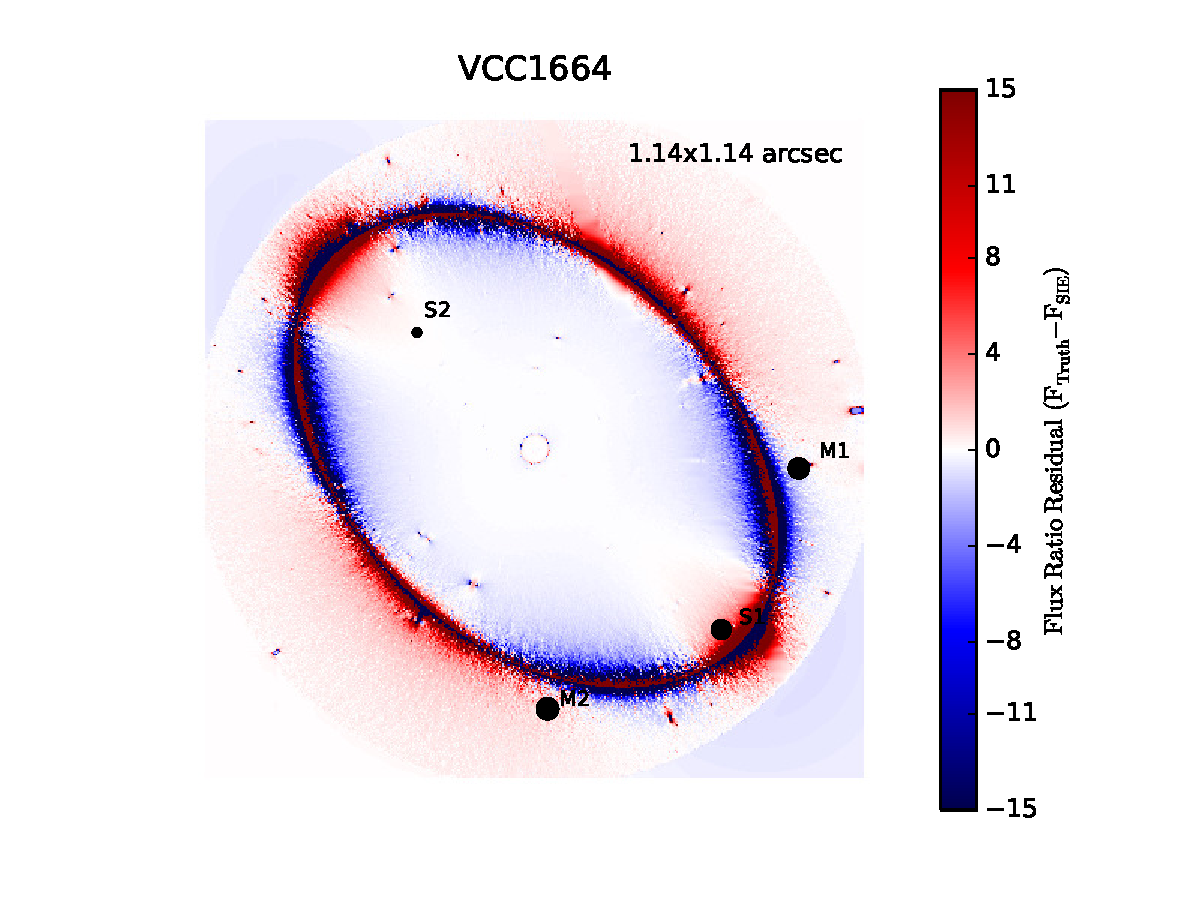
\includegraphics[clip,trim=2.5cm .5cm 1cm
		.25cm,width=0.48\linewidth,keepaspectratio]{./figures_sls/res_map_VCC1664_cusp_withshear-eps-converted-to.pdf}
		\caption[Map of magnification residuals for mock lens VCC1664]{\label{fig:magmaps_VCC1664} $R_{\rm{cusp}}$ anomaly. Left: Magnification surface derived from the convergence map. Right: Residuals after subtracting the magnification mag of the best fit SIE model. The effect of the stellar manifests itself as a multipole pattern in the residual map.}
	\end{figure*}
	\item VCC1692: An elongated galaxy with a prominent disk, as seen in Figure \ref{fig:fluxratios}, with stellar velocity dispersion $\sigma_* = 187 \ \rm{km/sec}$. We embed this galaxy in an external shear with a 60 degree offset between the disk position angle and the position angle of the external shear, resulting in a warped astroid caustic. The residuals between the magnification surface of the mock lens and the best fit SIE, shown in Figure~\ref{fig:magmaps_VCC1692c}, dramatically displays this effect, with large residuals on the ends of the disk where images are located. The lens has an unusual image configuration, with the far image (S2) located off the symmetry axis of the cusp, while the three cusp images are very close to each other. Both the SNFW and SIE fit the positions reasonably well, although both models display M1/S1 flux ratio anomalies of 80\%. The proximity of images M2 and S1 to the stellar disk likely significantly the perturbs the flux ratios between these images. We can compare this with the closest real analog in Figure~\ref{fig:Rcuspfold_vs_real} B2045+265. Deep imaging of the system \cite{McKean++07} shows that the deflector galaxy is almost perfectly round ($b/a=0.94\pm0.01$) when imaged with an F160W filter, while it displays irregular morphological features in F814W. \cite{McKean++07} also investigate the possibility that a luminous satellite located between the main deflector and the three cusp images could be responsible for the observed flux ratio anomaly. The Einstein radius of $1.06$ corresponds to a velocity dispersion of 278 km s$^{-1}$, once the correct source redshift of $z_s=2.35$ is taken into account (Nierenberg, 2017, private communication). Thus, the deflector galaxy in B2045 is very different than the one in the mock lens discussed here, consistent with a different origin of the anomaly, even though the amplitude is the same. In our sample of mock lenses, VCC1692 is the only lens with significant astrometric anomalies. In this sense it is an outlier, as our analysis shows that lensing by luminous matter typically does not result in image positions that cannot be fit by an SIE or SNFW, while they still may result in anamalous flux ratios. The interplay between the disk and external shear is likely to blame for this unique system, resulting in the asymmetric image configuration and peculiar shape of the astroid caustic. 
	\begin{figure*} 
		\centering
		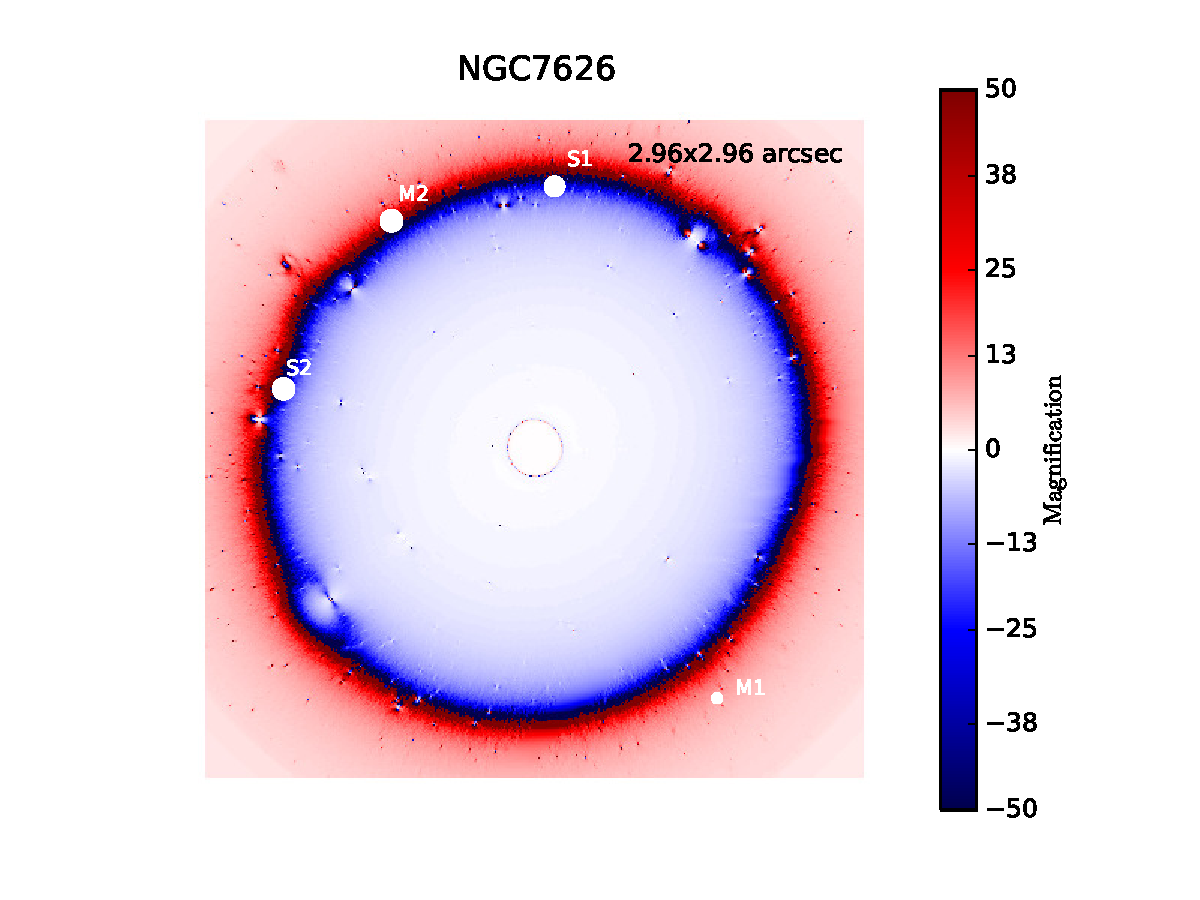
\includegraphics[clip,trim=2.5cm .5cm 1cm
		.25cm,width=0.48\linewidth,keepaspectratio]{./figures_sls/magmap_NGC7626_cusp_withshear-eps-converted-to.pdf}
		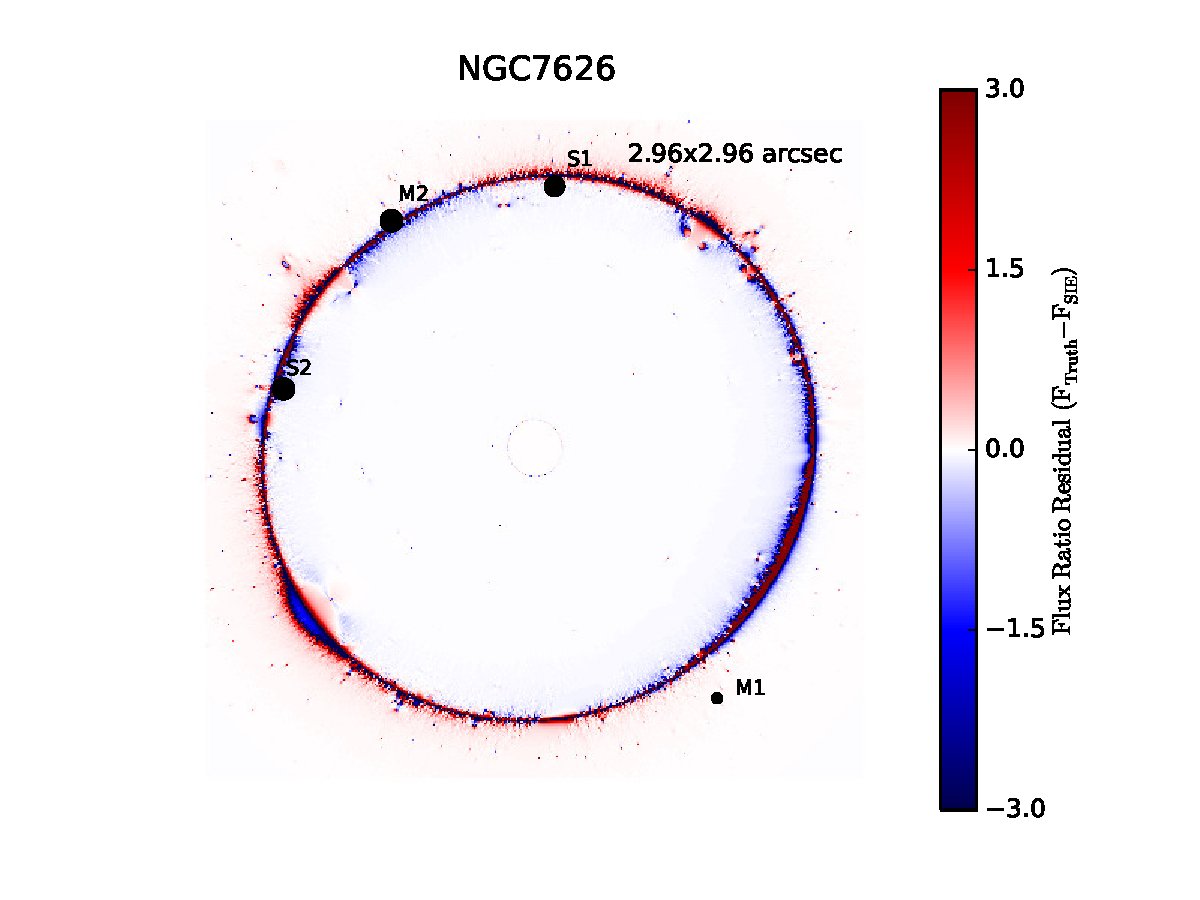
\includegraphics[clip,trim=2.5cm .5cm 1cm
		.25cm,width=0.48\linewidth,keepaspectratio]{./figures_sls/res_map_NGC7626_cusp_withshear-eps-converted-to.pdf}
		\caption[Map of magnification residuals for mock lens NGC7626]{\label{fig:magmaps_NGC7626} $R_{\rm{cusp}}$ anomaly. Left: Magnification surface derived from the convergence map. Right: Residuals after subtracting the magnification map of the best fit SIE model. This system does not exhibit any obvious large scale morphological irregularities, although the effect of a background galaxy in the lower left is clearly visible. The galaxy appears to contain many luminous substructures, some of which may be associated with a dark subhalo. However, it is possible that some of these features, such as the galaxy in the lower left, are in the background or foreground. In Section 3.3.1 we discuss the impact of luminous substructure on flux ratios and the $R_{\rm{cusp}}$ parameter.}
	\end{figure*} 
	\item VCC1664:  This is a small galaxy with velocity dispersion 155 km s$^{-1}$. As such, it is not representative of a typical deflector of lensed quasars. It is similar to VCC1692 in that it has a prominent disk that results in large M1/S1 and M2/S1 flux ratio anomalies that both the SIE and SNFW models fail to reproduce, as seen in the distributions of Figure \ref{fig:fluxratios2}. The magnification residuals between the \textit{Truth} model and the best fit SIE result in a multipole pattern around the critical curve, seen in Figure \ref{fig:magmaps_VCC1664}. Since there is a significant amount of small scale structure scattered around the deflector, some of which lay close to an image, we experimented with removing these potential sources of flux ratio anomaly, but found that this did not affect the flux ratios. A lens with a similar flux ratio anomaly, RXJ1131+1231 \cite{Sluse++03}, differs in several important ways. First, \cite{Suyu++13} measured a stellar velocity dispersion in J1131 of $323 \pm 23$ km s$^{-1}$, which would likely result in images far enough from the majority of the stellar mass of the lens to be affected by morphological features of the luminous matter, especially as imaging of J1131 shows no evidence for the presence of a stellar disk or significant elongation. Second, the flux ratio anomaly in J1131 is accompanied by an astrometric anomaly; attempts to fit the lens with an single SIE with shear or a two-lens model both fail to recover the correct astrometry, whereas smooth potentials recover the image positions of VCC1664 almost perfectly. It should also be noted that because VCC1664 has a larger cusp image separation $\theta$ than J1131, the $R_{\rm{cusp}}$ statistic can naturally be larger without substructure. 
	\begin{figure} 
		\centering
		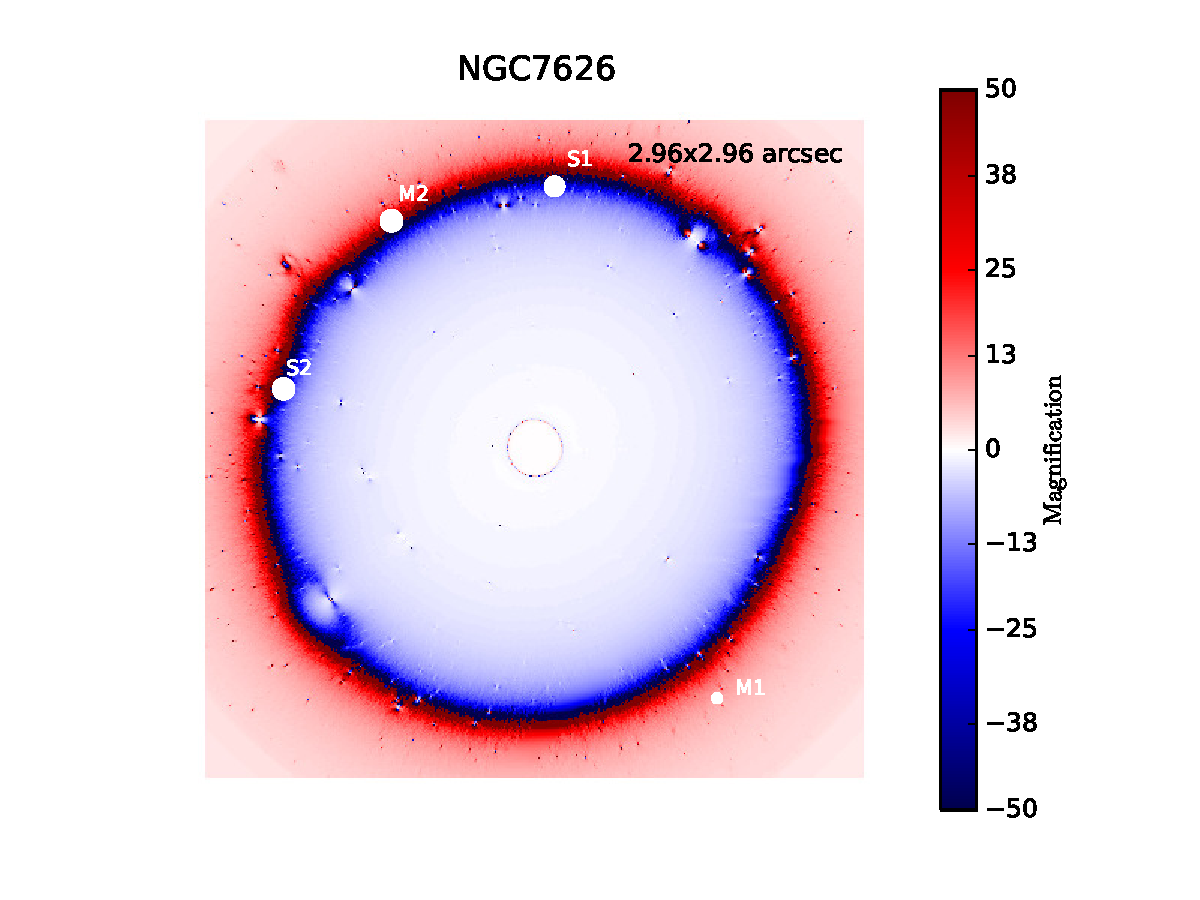
\includegraphics[clip,trim=2.5cm 6.5cm 10cm
		1.6cm,width=0.48\linewidth,keepaspectratio]{./figures_sls/magmap_NGC7626_cusp_withshear-eps-converted-to.pdf}
		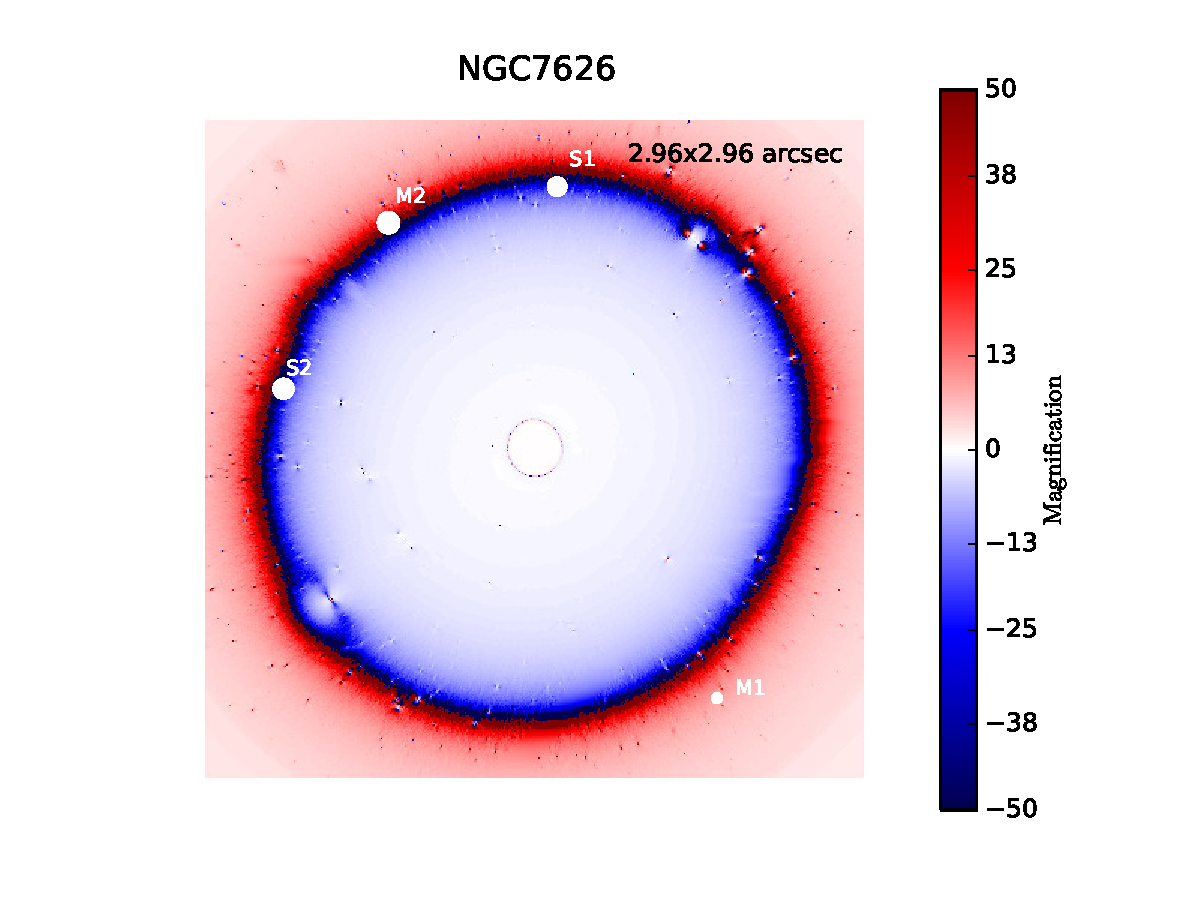
\includegraphics[clip,trim=2.5cm 6.5cm 10cm
		1.5cm,width=0.48\linewidth,keepaspectratio]{./figures_sls/magmap_nosat_after-eps-converted-to.pdf}
		\caption[Magnification map of NGC7626 with nearby galaxy removed]{\label{fig:magmaps_beforeafter} Left: Original magnification map, with all small scale structure present. Right: Magnification map with 3 globular clusters and one background or satellite galaxy removed. Before their removal, each of these features in the convergence map contributed the equivalent of $10^7 - 10^{7.5} M_{\odot}$.}
	\end{figure}
	\begin{figure} 
		\centering
		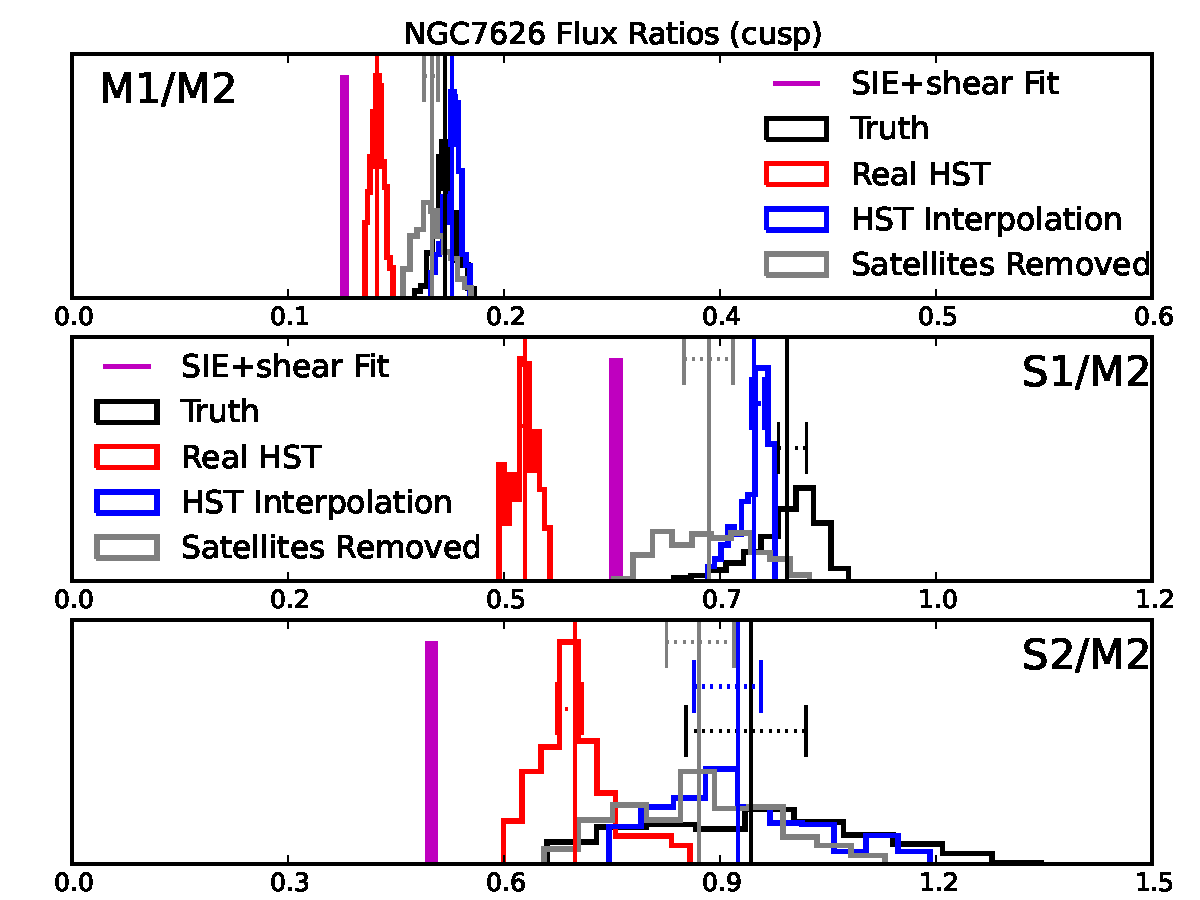
\includegraphics[clip,trim=0.5cm 0cm 0.5cm
		5.55cm,width=0.75\textwidth,keepaspectratio]{./figures_sls/nosatellites_fluxratiosdistributions2-eps-converted-to.pdf}
		\caption[Flux ratio distributions for NGC7626 with nearby galaxy removed]{\label{fig:newfluxratios} Flux ratios after the removal of small scale structure between the three cusp images in NGC7626.}
	\end{figure}
	\item NGC7626: This is the most massive cusp mock lens 
	($\sigma_* = 274$ km sec$^{-1}$) with a significant $R_{\rm{cusp}}$ anomaly. NGC7626 is surrounded by globular clusters and luminous satellites. One background galaxy is visible to the lower left, and it induces a flux ratio anomaly in the fold configuration (see the S2/M1 ratio in Figure \ref{fig:fluxratios}), although it is too far from the cusp images to be responsible for the $R_{\rm{cusp}}$ anomaly and does not affect the merging pair in the fold configuration. There are two structures between the M2 and S2 images, seen clearly in the convergence map (Figure \ref{fig:fluxratios}) and in the map of the magnification surface (Figures \ref{fig:magmaps_NGC7626} and \ref{fig:magmaps_beforeafter}) which visibly perturb the critical curve. The structure outside the curve resembles a background spiral galaxy, while the object just inside resembles a large globular cluster. Since NGC7626 does not possess a stellar disk or boxy isophotes that could explain the anomaly, we experimented with removing these features individually, replacing them with smooth interpolations of the convergence map. Specifically, we removed the globular cluster and background galaxy between M2 and S2, a small globular cluster near S1, and a very small cluster near S2. The before/after magnification maps are shown in Figure \ref{fig:magmaps_beforeafter}, and the new flux ratios in Figure \ref{fig:newfluxratios}. After removing these small scale structures, which our normalization procedure assigned convergence equivalent to that produced by a $10^7 M_{\odot}$ perturber, we find that the $R_{\rm{cusp}}$ anomaly shrinks in magnitude to 0.19 from 0.26. In the context of Figure \ref{fig:poserr_vs_Rcuspfold}, this suggests it could be accounted for by an SIE model. We therefore conclude that the main source of anomaly in this system is due to structure in the deflector on scales smaller than the image separation. This hypothesis is supported by examining the residual map in Figure \ref{fig:magmaps_NGC7626}, where the alternating blue and red colors coincide with the location of the perturbing globular clusters and galaxy. NGC7626 highlights that even massive deflectors can suffer flux ratio anomalies if there is sufficient small scale structure near the critical curve, whether it is in the form of dark substructure or luminous matter. However, it is important to remember that that this is seemingly a rare occurrence, and it is possible that this signal will be overwhelmed by the lensing signatures of a full population of dark subhalos, a question we will address in a future paper. 
	
	\vspace{1cm} In the $\theta$ vs. $R_{\rm{cusp}}$ parameter space, RXJ0911+0551 \cite{Kneib++00} is the nearest neighbor of NGC7626. NGC7626 is a round deflector with an ellipticity of 0.17, while a best fit SIE model of J0911 \cite{Sluse++12} favors a deflector with ellipticity 0.11. The velocity dispersion of J0911, if it is modeled as an SIE with Einstein radius 0.9 arcsec works out to $\sigma_{\rm{SIE}}=239$km s$^{-1}$ after adopting correct lens and source redshifts \cite{Kneib++00}, while NGC7626 has a velocity dispersion of 274 km s$^{-1}$. Neither J0911 nor NGC7626 display astrometric anomalies with respect to a smooth model when a second deflector galaxy is included in the model for J0911 \cite{Sluse++12}. NGC7626 stands out in our set of mock lenses, as it is round with high velocity dispersion, but still displays significant flux ratio anomalies, indicting that high velocity dispersion does not always guarantee benign flux ratios.  
	\begin{figure*} 
		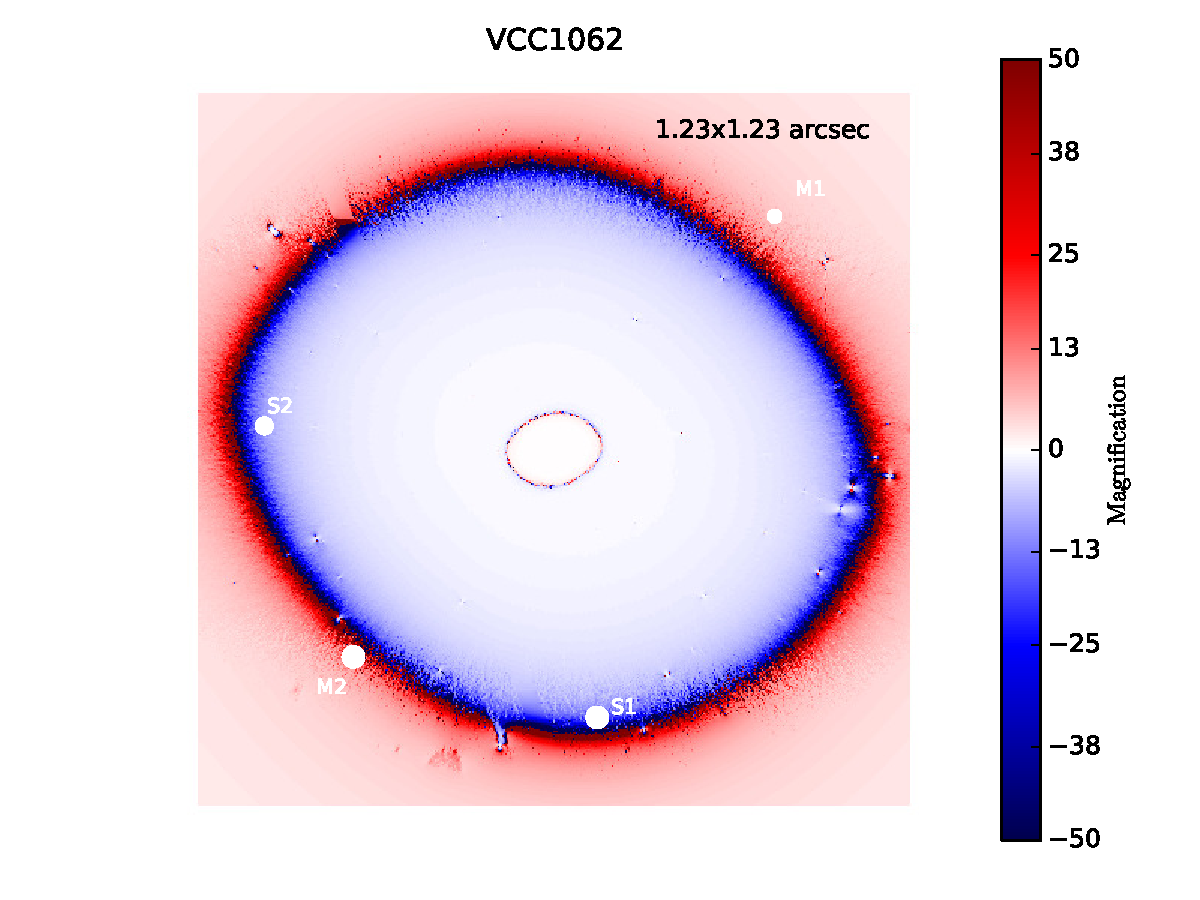
\includegraphics[clip,trim=2.5cm .5cm 1cm
		.25cm,width=0.48\linewidth,keepaspectratio]{./figures_sls/magmap_VCC1062_cusp_withshear-eps-converted-to.pdf}
		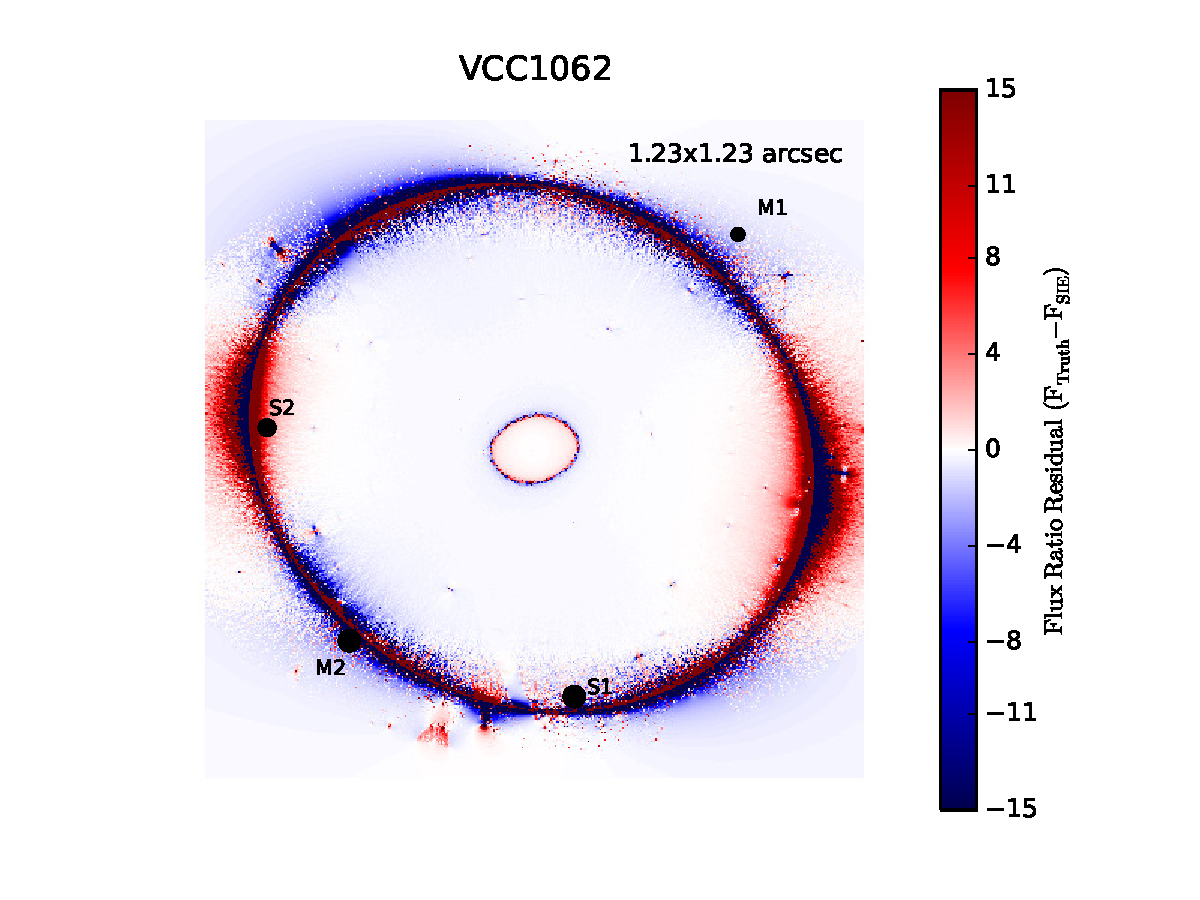
\includegraphics[clip,trim=2.5cm .5cm 1cm
		.25cm,width=0.48\linewidth,keepaspectratio]{./figures_sls/res_map_VCC1062_cusp_withshear-eps-converted-to.pdf}
		\caption[Map of magnification residuals for mock lens VCC1062]{\label{fig:magmaps_VCC1062} $R_{\rm{cusp}}$ anomaly. Left: Magnification surface derived from the convergence map. Right: Residuals after subtracting the magnification mag of the best fit SIE model. The effect of the stellar mass manifests itself as a multipole pattern in the residual map.}
	\end{figure*}
	\item VCC1062: The external shear applied in this lens forms an angle of 61 $\deg$ with the stellar quadrupole moment position angle, similar to VCC1692, that results in a cusp configuration that is not coaxial with the stellar ellipticity position angle. Coupled with the boxy isophotes (see Figure \ref{fig:C0_vs_Rcuspfold}), this results in a complicated potential that the best fit SIE fails to capture, as seen in the map of flux ratio residuals in Figure \ref{fig:magmaps_VCC1062}. 
	\begin{figure*}
		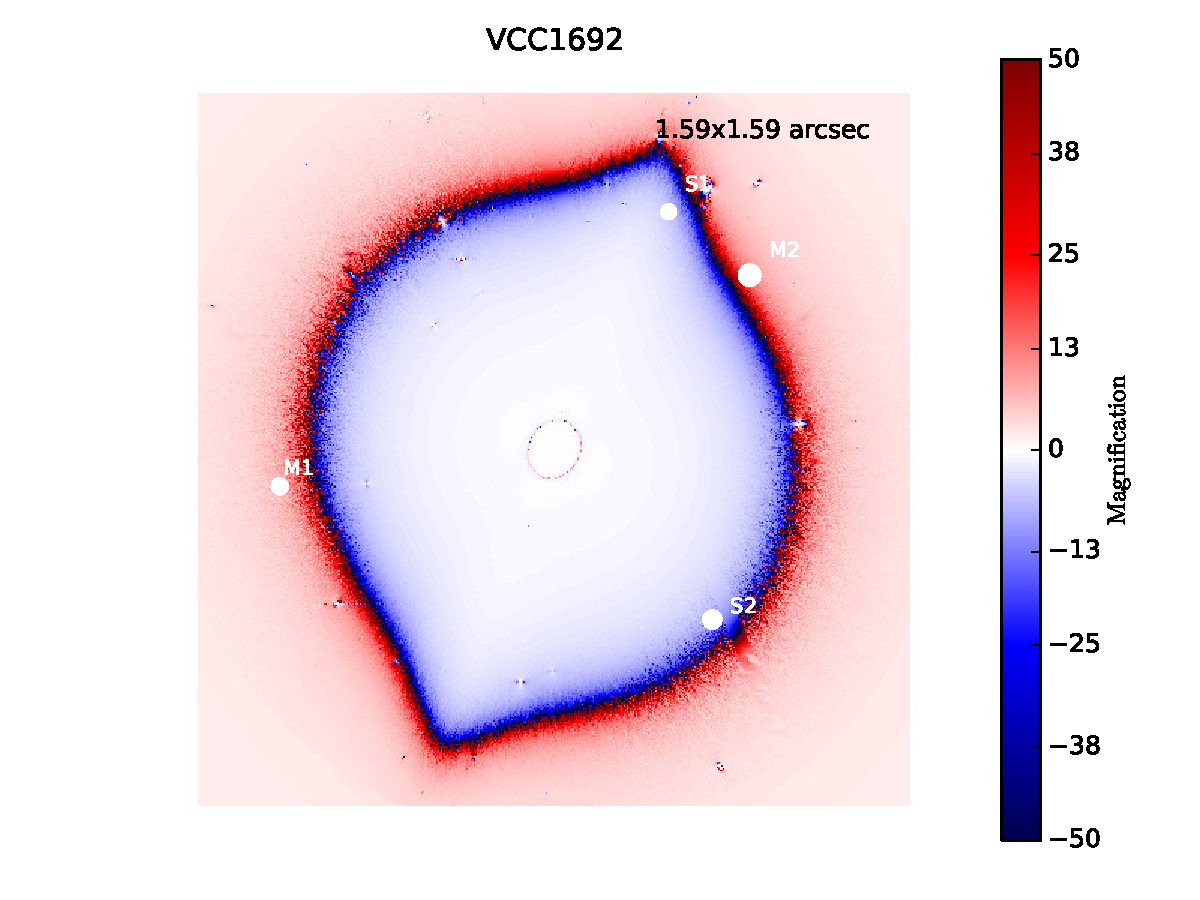
\includegraphics[clip,trim=2.5cm .5cm 1cm
		.25cm,width=.48\textwidth]{./figures_sls/magmap_VCC1692_fold_withshear-eps-converted-to.pdf}
		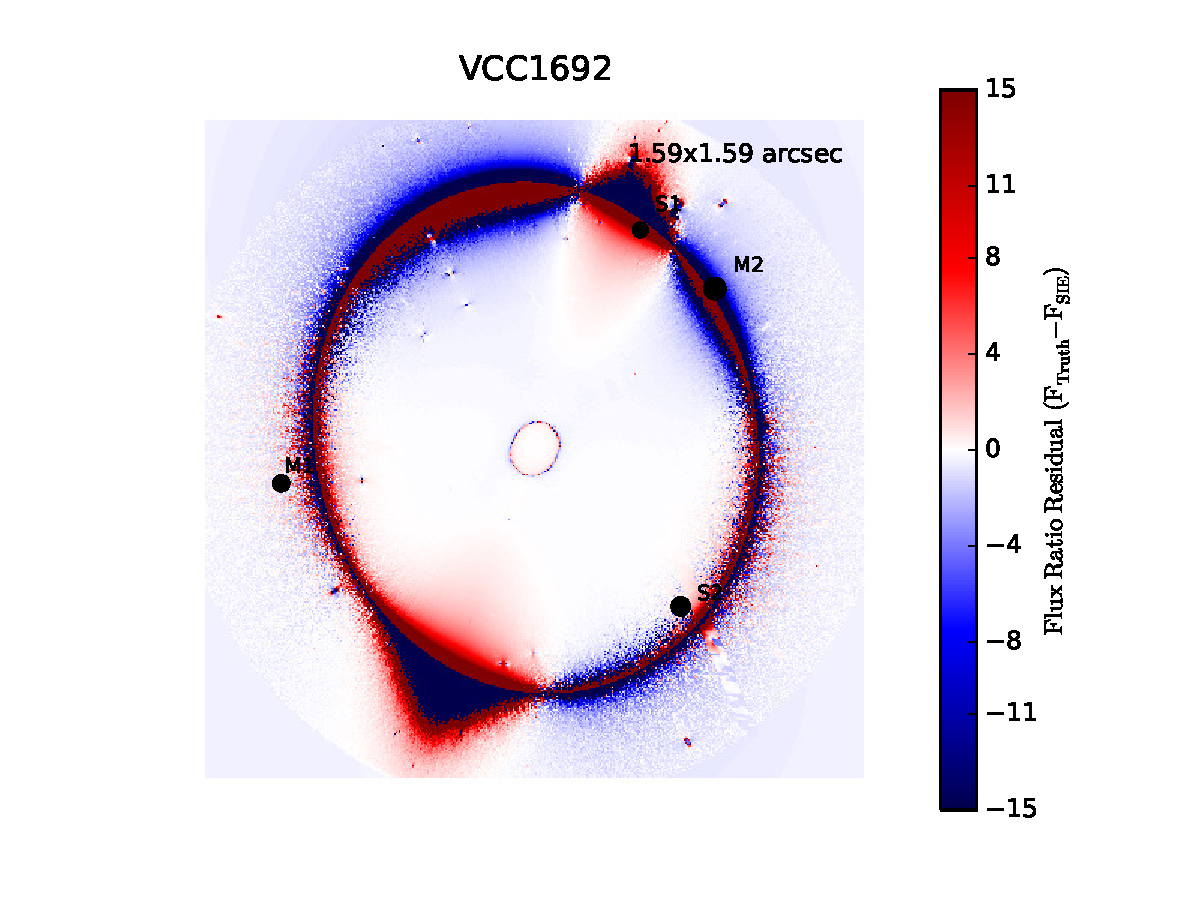
\includegraphics[clip,trim=2.5cm .5cm 1cm
		.25cm,width=.48\textwidth]{./figures_sls/res_map_VCC1692_fold_withshear-eps-converted-to.pdf}
		\caption[Map of magnification residuals for mock lens VCC1692]{\label{fig:magmaps_VCC1692f} $R_{\rm{fold}}$ anomaly. Left: Magnification surface derived from the convergence map. Right: Residuals after subtracting the magnification mag of the best fit SIE model. The merging image pair in this fold configuration happens to land near the portion of the critical curve extended by the stellar disk, a feature the best SIE fails to capture. The resulting residual in the magnification surface gives rise to the large $R_{\rm{fold}}$ anomaly.} 
	\end{figure*}
	\vspace{1cm}  The small velocity dispersion ($\sigma_* = 179$ km/sec) results in a small Einstein radius, which in turn results in images close to the center of the lens. As a result, the images S2 and M2 are located closer to the ends of the elongated baryonic mass distribution where there is more curvature in the potential, making this lens more susceptible to influence from its luminous mass component. While both the SIE and SNFW fail to recover the correct flux ratios, the anomalies are $<40\%$. However, collectively the anomalies lead to a significant $R_{\rm{cusp}}$ anomaly. VCC1062 has an anomaly quite similar to that observed in B0712+472 \cite{Jackson++98}. Both deflectors have relatively small stellar velocity dispersion (B0712 has $\sigma_{\rm{SIE}} = 189$ km/sec), which we estimate for B0712 by adopting the correct redshifts as cited in \cite{Sluse++12} and utilizing the relationship between image separation and velocity dispersion presented in \cite{Kochanek++00}. The two lens systems both appear to have highly elliptical baryonic mass distributions, consistent with the presence of edge-on massive disk \cite{Jackson++98}. While the small mass and high ellipticity of B0712 suggests the anomaly may be influenced by baryonic matter, the astrometric anomaly noted by \cite{Kawano++04} is not a common feature among our mock lenses, and as such alternate explanations are favored, such as dark substructure. Discrepancies between the flux ratios in the optical/near IR and radio data suggest microlensing and/or dust extinction could also be present. Regardless, deeper imaging of this system could help disentangle the possible role of baryonic structure from other sources of flux ratio perturbation. 
	
	\vspace{1cm} Completely different is the case of the real lens B1422+231 \cite{Patnaik++92}. Even though the cusp flux ratio anomaly is similar to that of VCC1062, the cusp image separation $\theta$ is large enough that the measured $R_{\rm{cusp}}$ value \cite{Koopmans++03} alone is not inconsistent with lensing by a smooth potential \cite{Keeton03}, while the analysis by \cite{Nierenberg++14,Xu++15} suggests substructure in the vicinity of image A could contribute to the anomaly. Like many systems in our sample, the astrometric anomalies in B1422 are relatively tame compared to other real lens systems.
\end{itemize}
\subsubsection{\rm{FOLDS}}

\begin{itemize}
	
	\item VCC1692: The only significant $R_{\rm{fold}}$ anomaly appears in VCC1692, the lens system with the largest $R_{\rm{cusp}}$ anomaly. The S1/M2 flux ratio anomaly is 50\%, likely because of the influence of the stellar disk. This effect is clear in Figure~\ref{fig:magmaps_VCC1692f}, where large residuals between the best fit SIE and the \textit{Truth} model are evident. Unlike the cusp configuration, the \textit{HST Interpolated} distribution agrees with the \textit{Truth} flux ratios, indicating that the curvature of the gravitational potential just off the major axis of the disk is gradual enough that the convolution procedure still captures the disk's effect on the magnification surface. From a modeling standpoint, this implies that the information needed to accurately reproduce the lensing signal of a very disky deflector is lower for fold configurations than for cusp configurations, because cusps images live near the ends of the disk (for major axis cusps), where there is greater curvature. Conversely, folds will tend to straddle the sides of a disk, so one need only resolve a small portion of a relatively straight critical curve dividing the two images.
	
	\vspace{1cm} B1555+375 \cite{Marlow++99}, the closest real analogue to VCC1692 in the $R_{\rm{fold}}$ / $\theta_1$ parameter space, has a nearly identical $\theta_1$ and a large $R_{\rm{fold}}$. B1555 is also a very small angular separation lens, with a deflector velocity dispersion estimated from the image separation of 134 km s$^{-1}$, and is highly elliptical. The high ellipticity $\epsilon = 0.54$ and disk feature detected in deep AO imaging \cite{Hsueh++16} further strengthen the analogy between the mock and the real system. Attempts to model the lens system \cite{Marlow++99,MirandaJetzer07} also find that the astrometry of B1555 is consistent with an SIE model, so no extreme astrometric anomalies are present, as is the case with the majority of our mock lenses. Another clue to the nature of the anomaly in B1555 arises from the modeling of VCC1692: if flux ratios are included as constraints in the SIE fit to VCC1692, the resulting astrometric errors and flux ratios appear strikingly similar to that observed in B1555. This suggests that, while formally not a good fit to the data, a single SIE can capture the astrometry and flux ratios of a disky galaxy to within 10 mas and $\approx 70 \%$, respectively. It is likely that this is not a coincidence, as \cite{Hsueh++16} show that the system can be fit to high precision by explicitly modelling the stellar disk, without the need to invoke dark subhalos. Naturally, this does not mean that dark substructure is not present, just that it is not required.
	
	\vspace{1cm} The lens system MG0414+0534 is not fit for juxtaposition with VCC1692, as the central velocity dispersion, derived from the Einstein radius of an SIE \cite{Xu++15}, is approximately 286 km s$^{-1}$, while lens models favor moderate SIE ellipticity of $\approx 0.2$, indicating that the lensing galaxy is likely very massive and round \cite{Hewitt++92}. While the anomaly is small in magnitude, the proximity of the merging image pair makes it unlikely that a smooth potential provides an adequate description of the lens system \cite{Minezaki++09,Keeton05,Xu++15}. However, \cite{Xu++15} point out that other sources of anomaly besides dark substructure may be needed to explain the observed anomaly. Deep imaging of this system would help rule out the possibility that baryons play a significant role, although the non-detection of baryon-induced $R_{\rm{fold}}$ anomalies in our sample suggests the dark matter is responsible. 
	
	\vspace{1cm} B0128+437 \cite{Phillips++00}, a small deflector with $R_{\rm{Ein}}=0.24"$, and low sersic index, consistent with a late-type morphology \cite{Lagattuta++10}. \cite{Biggs++04} show that lens models favor very elliptical SIE profiles, but fail to fit the observed image positions. While the small size of the lens and elongated nature of the deflector suggest baryons may contribute a non-negligible effect to the flux ratios, the presence of astrometric anomalies suggests non-baryonic substructure may also contribute.
	
	The system B1608+656 \cite{Fassnacht++96} is peculiar in that it consists of two merging galaxies \cite{Fassnacht++02}, with the most massive one having a velocity dispersion of $260\pm15$ km s$^{-1}$ \cite{Suyu++10}. The B1608 system is complex enough that a  description in terms of simple anomalies is not appropriate and searches for dark matter substructure must take into account this complexity with a detailed model.
	
	Even more anomalous than any one of our mock lenses is the system B1933+503 \cite{Skyes++98}, a well known peculiar system with a late-type deflector that contains a prominent stellar disk. \cite{KochanekDalal04} investigate whether higher order multipole terms in the lens potential can account for the observed anomaly, and conclude that such an explanation is unlikely, which seems to favor a dark substructure as a source of flux ratio perturbation. However, it is possible that the lensing properties of galaxies with very irregular morphology, such as a prominent edge on disk, may require a more different description than can be encapsulated by adding a few higher order multipole terms.
	\begin{figure*}
		\centering
		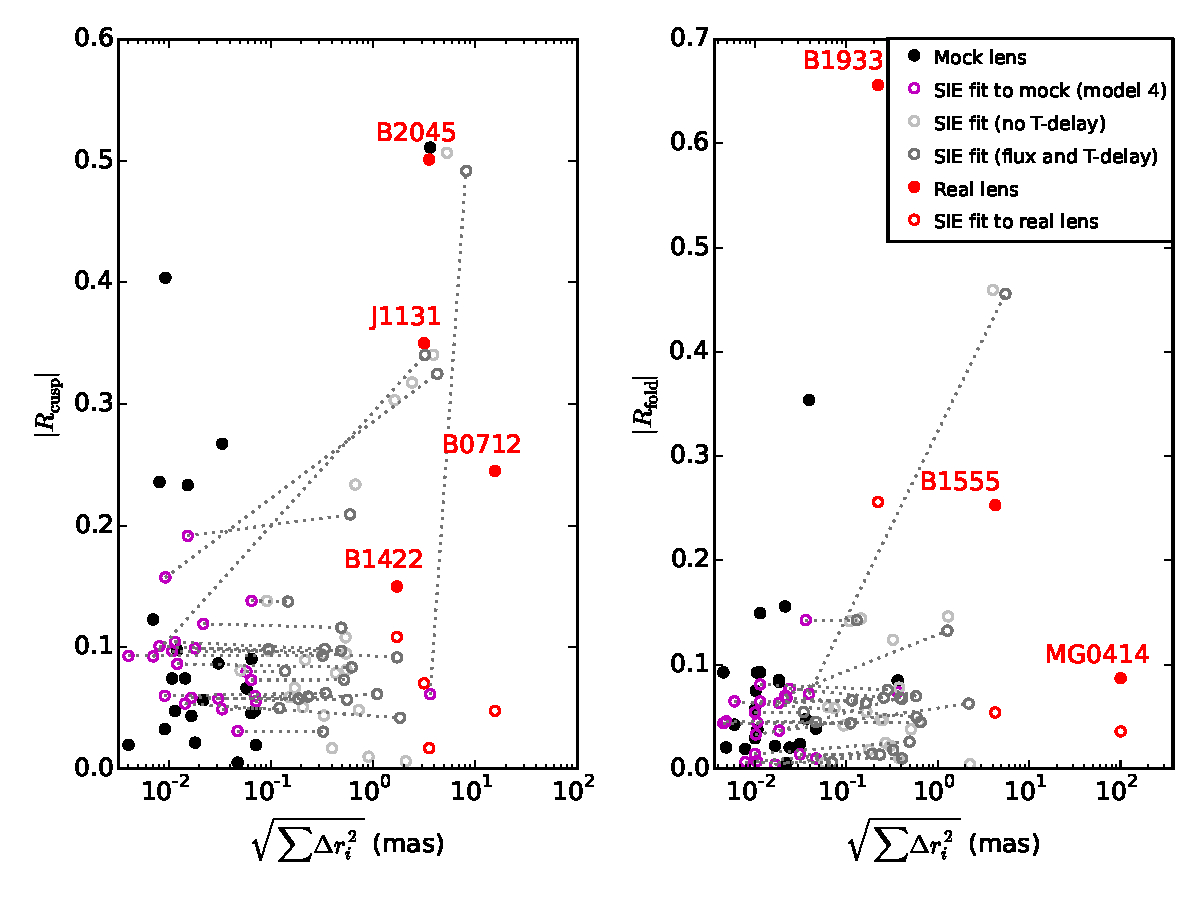
\includegraphics[trim=0cm .5cm 0cm .4cm,clip,width=.7\textwidth]{./figures_sls/poserror_vs_Rcuspfold_withlines-eps-converted-to.pdf}
		\caption[$R_{\rm{cusp}}$ and $R_{\rm{fold}}$ statistics]{\label{fig:poserr_vs_Rcuspfold} $R_{\rm{cusp}}$ and $R_{\rm{fold}}$ parameters for the \textit{Truth} model and best fit SIE \textit{Truth} model (black points and purple circles, respectively), together with the values observed in real lenses (red points), and SIE fits to real lenses (red circles). The real lenses and \textit{Truth} data points are distributed along the x-axis according to the astrometric error of their best fit SIE model summed in quadrature. Counter-intuitively, as most of our mock lenses have R values larger than the best fit SIE, a positively sloped dashed line is actually an improved model for the data, although the R value increases. This flux ratio precision comes at a cost of larger astrometric and time-delay errors, irrespective of the exact uncertainty we place on the flux ratios and time delays. Further, without time delay information (light grey points), the code cannot distinguish between major and minor axis cusps, which further complicates the modeling process. In this plot, we impose flux ratio uncertainties of 10 \% (grey points). When fitting the real lens systems, we adopt lens data and observational uncertainties from \cite{Sluse++12} (MG0414, B2045), \cite{Sluse++06} (J1131), \cite{Jackson++98} (B0712), \cite{Nierenberg++14} (B1422), \cite{Cohn++01} (B1933), and \cite{Hsueh++16} (B1555). There is a clear separation between the real lenses and the
			mock lenses, with real systems possessing both astrometric
			and  flux ratio anomalies, and our set of mock lenses mostly
			confined to  flux ratio anomalies $<$ 30\% and nearly perfect
			astrometric precision.}
	\end{figure*}
\end{itemize}
The possibility of a large $R_{\rm{cusp}}$ or $R_{\rm{fold}}$ arising from the baryonic structure of the lens, especially in low mass ellipticals with features such as disks or boxy isophotes, behooves observers to investigate whether the lensing galaxy possesses baryonic mass distributions that require detailed modeling. Indeed, deep imaging of B1555 and B0712 shows that a disk is present, and can account for the apparent anomaly \cite{Hsueh++16}. Of the lenses in our sample with the largest $R_{\rm{cusp}}$ values, some have stellar disks visible even in the rebinned images. Others do not have visible disks but are significantly elongated, even in the rebinned images. These findings suggest that in most cases an elliptical galaxy at $z=0.5$ can be imaged well enough by the HST for potential sources of baryonic anomaly to be identified and modeled, but care should be taken to account for the interplay between the external shear and stellar ellipticity, which could result in an off-axis cusp, as in VCC1692 and VCC1062 imaged in Figures \ref{fig:fluxratios} and \ref{fig:fluxratios2}.

\subsubsection{Characterizing a baryonic-lensing signal through modeling: astrometric and flux ratio anomalies}  

Among the properties of the baryonic mass of a deflector likely to give rise to flux ratio anomalies, stellar disks or other elogated structures, most often seen in low mass, low stellar velocity dispersion galaxies, constitute the majority of the anomalous systems in our sample. On the other hand, in round, high velocity dispersion systems such as NGC7626 where there is no obvious stellar disk or other large scale feature, anomalies could be induced by compact structures near the critical curve. Regardless of the origin, flux ratio anomalies from luminous matter may be difficult to identify solely by examining flux ratios.
\newline \indent In order to help distinguish a baryonic lensing signal in systems similar to NGC7626 from other sources of anomaly, we highlight a feature of our mock systems, seen even systems with significant flux ratio anomalies, that is not frequently observed in real lens systems. Our mock lenses are characterized by a conspicuous absence of astrometric anomalies, which can be present in real systems at the level of tens of mas for subhalos located near an image, in projection \cite{Chiba02,Chen++07}. This suggests that a feature of perturbation by dark matter subhalos, that could be used to distinguish between baryonic and dark matter perturbations, is a flux ratio anomaly coupled to an astrometric anomaly, especially if the introduction of a dark substructure to the lens model simultaneously resolves both discrepancies.   
\newline \indent To compare the astrometric precision of the SIE model fit to our mock lenses with that of an SIE fit to real  lenses, we fit several of the real systems shown in Figure \ref{fig:Rcuspfold_vs_real} with an SIE plus external shear, varying the Einstein radius, ellipticty, shear, position angles, and deflector centroid. For the resulting best fit model we compute the flux ratio and astrometric anomalies. We omit systems such as J0911 and B1608, which require complicated modeling involving two galaxies within the Einstein radius. We repeat the fit for each of our mock systems omitting time delays and enforcing flux ratio constraints, to see if the inclusion or exclusion of either these data significantly impacts the results.
\begin{figure*}
	{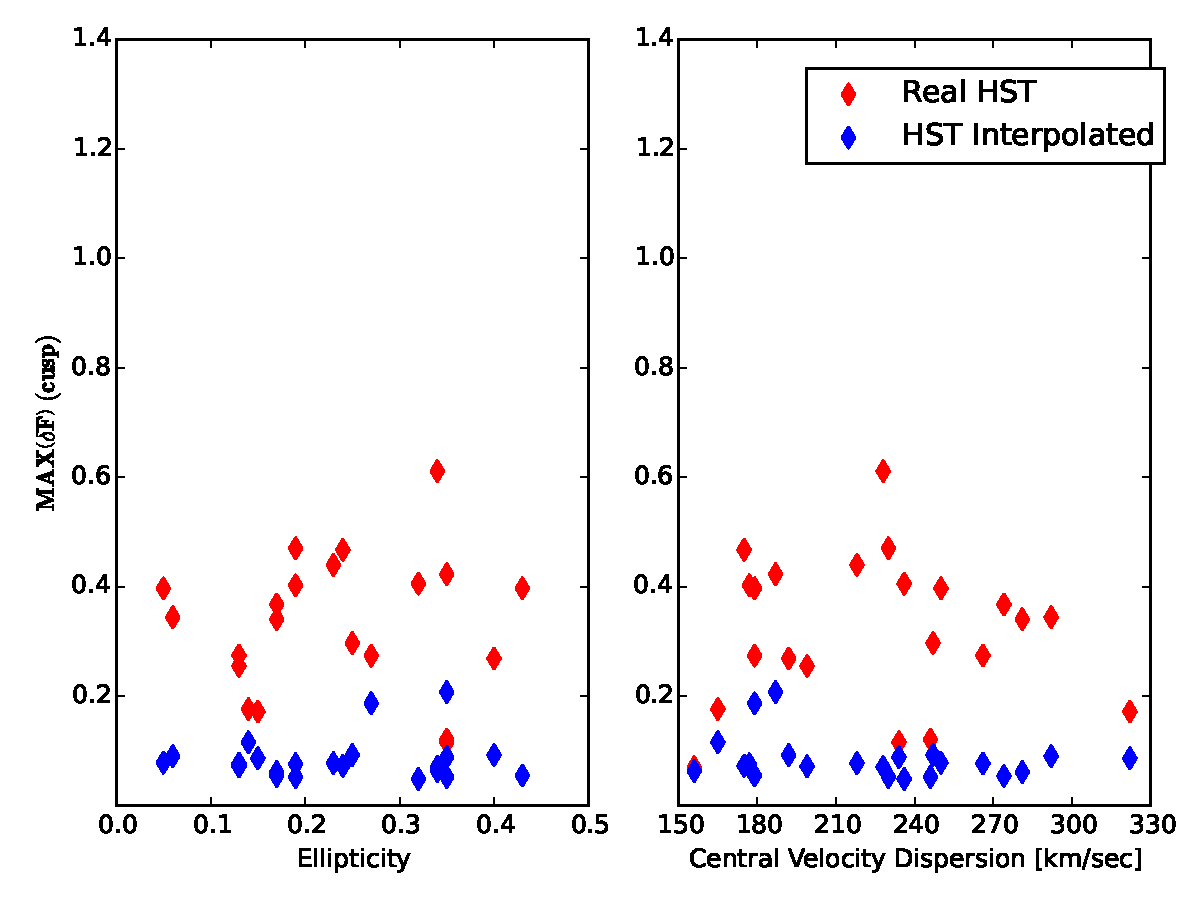
\includegraphics[trim=0cm 0cm 0cm
		0cm,clip,width=.48\textwidth]{./figures_sls/EllipVdis_vs_fluxratio_maxanomaly_cusprebinsmooth-eps-converted-to.pdf}}
	{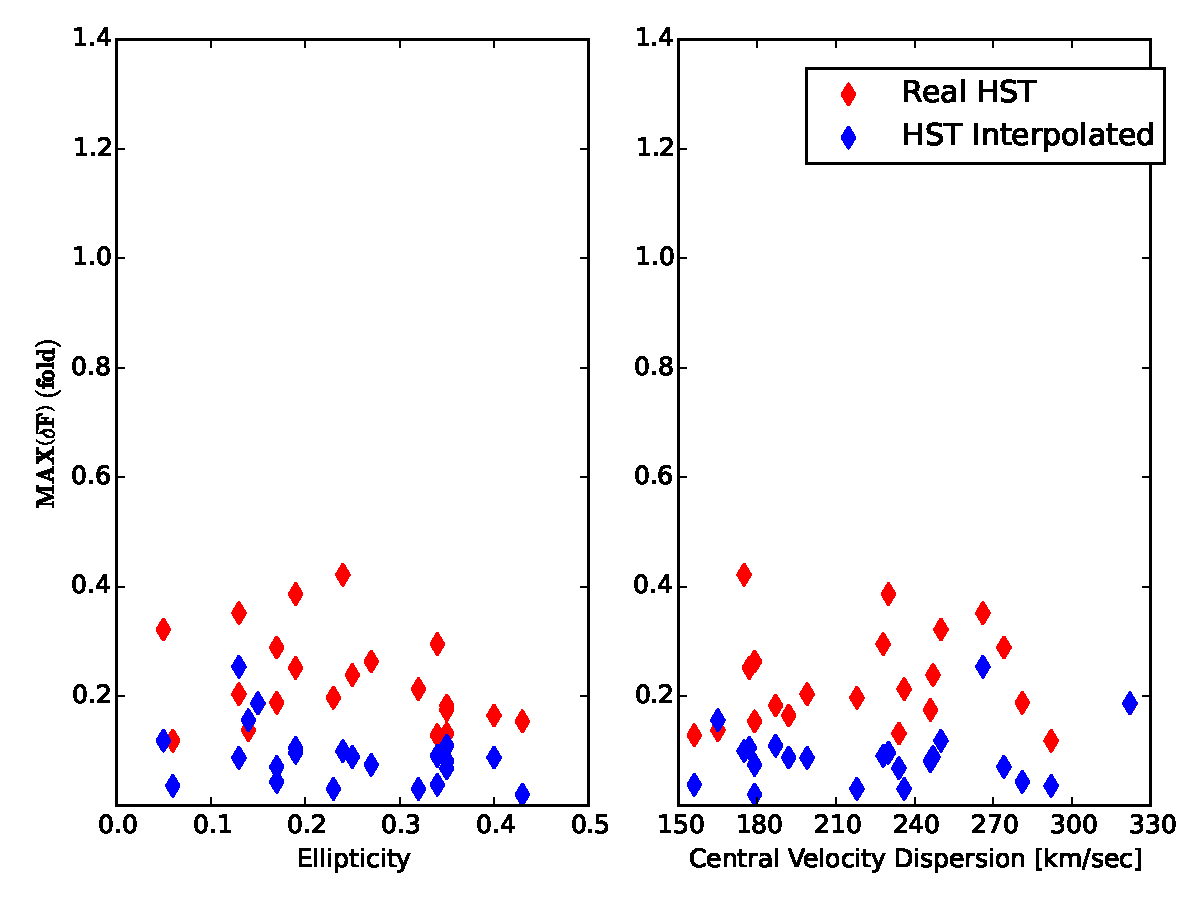
\includegraphics[trim=0cm 0cm 0cm
		0cm,clip,width=.48\textwidth]{./figures_sls/EllipVdis_vs_fluxratio_maxanomaly_foldrebinsmooth-eps-converted-to.pdf}}
	\caption[The largest flux ratio anomaly for \textit{Real HST} and \textit{HST Interpolated} models as a function of ellipticity and central velocity dispersion]{\label{fig:fluxratios_23}Largest flux ratio anomaly for Model 2 (\textit{Real HST}) and Model 3 (\textit{HST Interpolated}) in each lens as a function of ellipticity and central velocity dispersion for cusp configurations (left) and fold configurations (right).}
\end{figure*}
\begin{figure*}
	{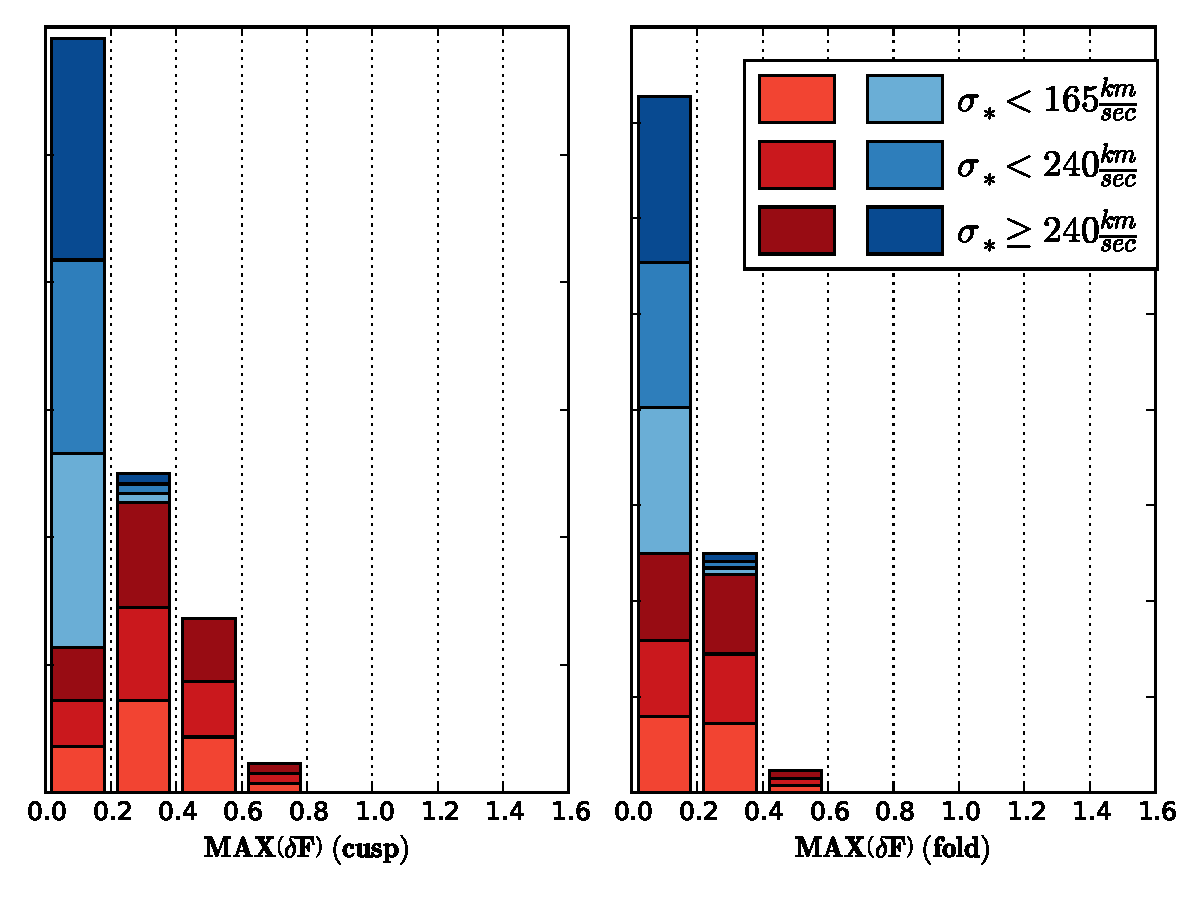
\includegraphics[trim=0cm 0cm 0cm .3cm,clip,width=8.5cm, height=6.85cm]{./figures_sls/maxanomaly_disrebinsmooth-eps-converted-to.pdf}}
	{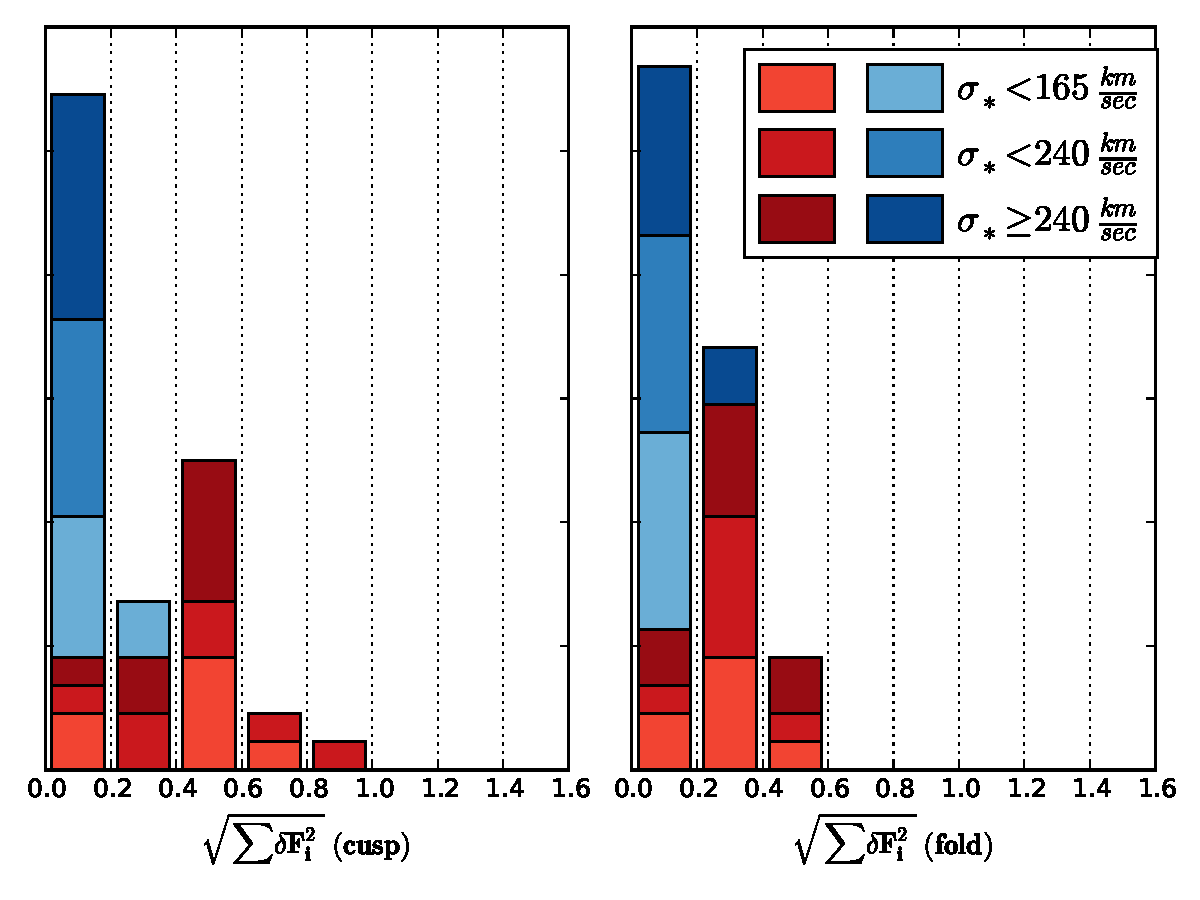
\includegraphics[trim=0cm 0.2cm 0cm 0cm,clip,width=8.5cm, height=7cm]{./figures_sls/sumquad_disrebinsmooth-eps-converted-to.pdf}}
	\caption[Distributions of the largest flux ratio anomalies for \textit{Real HST} and \textit{HST Interpolated} models]{\label{fig:distribution_23}Distributions of the largest anomalies (left) and the three anomalies summed in quadrature (right) for each lens, color coded by the deflector's central velocity dispersion. The color scheme is the same as in Figure~\ref{fig:fluxratios_23}.}
\end{figure*} 
\begin{figure*}
	{\includegraphics[trim=0cm 0.3cm 0cm 0.3cm,clip,width=.48\textwidth]{./figures_sls/EllipVdis_vs_fluxratio_maxanomaly_cusp-eps-converted-to.pdf}}
	{\includegraphics[trim=0cm 0.3cm 0cm 0.3cm,clip,width=.48\textwidth]{./figures_sls/EllipVdis_vs_fluxratio_maxanomaly_fold-eps-converted-to.pdf}}
	\caption[Largest flux ratio anomalies as a function of ellipticity and central velocity dispersion for the smooth model fits]{\label{fig:fluxratios_45}Largest flux ratio anomaly for Model 4 (purple) and Model 5 (green) in each lens as a function of ellipticity and central velocity dispersion for cusp configurations (left) and fold configurations (right).}
\end{figure*}
\begin{figure*}
	{\includegraphics[trim=0cm 0.2cm 0cm 0.3cm,clip,width=8.5cm, height=6.85cm]{./figures_sls/maxanomaly_dis-eps-converted-to.pdf}}
	{\includegraphics[trim=0cm 0.2cm 0cm 0.3cm,clip,width=8.5cm, height=7cm]{./figures_sls/sumquad_dis-eps-converted-to.pdf}}
	\caption[Distributions of largest flux ratio anomalies for the smooth model fits]{\label{fig:distributions_45}Distributions of the largest anomalies (left) and the three anomalies summed in quadrature (right) for each lens, color coded by the deflector's central velocity dispersion. The color scheme is the same as in Figure~\ref{fig:fluxratios_45}}
\end{figure*}
\begin{figure*}
	{\includegraphics[trim=0cm 0.2cm 0cm 0.2cm,clip,width=.48\textwidth]{./figures_sls/EllipVdis_vs_Rcusp-eps-converted-to.pdf}}
	{\includegraphics[trim=0cm 0.2cm 0cm 0.2cm,clip,width=.48\textwidth]{./figures_sls/EllipVdis_vs_Rfold-eps-converted-to.pdf}} 
	\caption[$R_{\rm{cusp}}$ and $R_{\rm{fold}}$ statistics for the fits versus the \textit{Truth} model]{\label{fig:Rcuspfold_plot}Differences in the R-cusp (left) and R-fold (right) statistics between the SIE and SNFW models, and the \textit{Truth} data. The color scheme is the same as in Figure \ref{fig:fluxratios_45}.}
\end{figure*}
\newline \indent In Figure \ref{fig:poserr_vs_Rcuspfold}, we plot the $R_{\rm{cusp}}$ or $R_{\rm{fold}}$ values of our mock lenses and some real lens systems, along with a best fit SIE to each of the real systems and mocks as a function of the total astrometric error summed in quadruature. There is a clear separation between the real lenses and the mock lenses, with real systems possessing both astrometric and flux ratio anomalies, and our set of mock lenses mostly confined to flux ratio anomalies $\leq 30 \%$ and nearly perfect astrometric precision. The effect is more pronounced in cusp lenses, although both image configurations follow this general trend. Enforcing flux ratio contraints of 10 \% in the SIE fit to the mock lenses sometimes corrects the flux ratio anomaly at the expensive of astrometric precision, but the resulting points still populate a different region of parameter space than the real lens systems. Additionally, while SIE fits to the mock lenses systems come close to reproducing the observed $R_{\rm{cusp}}$ or $R_{\rm{fold}}$ value, the best fit model of a real lens system differs significantly.
\newline \indent Our analysis aims to characterize the properties of a deflector (low velocity dispersion, high ellipticity, etc.) that may increase the likelihood of observing a baryon-induced flux ratio anomaly. While the trend in Figure \ref{fig:poserr_vs_Rcuspfold} can be used to characterize a purely baryonic lensing signal by the absence of an astrometric anomaly, it should not be adopted as a criterion used to rule out lens systems as candidates for analysis of dark matter substructure, as our analysis does not address the question of whether a dark subhalo will necessarily result in simultaneous astrometric and flux ratio anomalies, and the relative magnitudes of these perturbations. Further, the interpretation of what constitutes an astrometric anomaly is model dependent, and depends on the precision the available data. Regardless of these nuances, given a large sample of lenses, observations of the morphological features of the lensing galaxy, together with an absence of astrometric anomalies in the presence of relatively small flux ratio anomalies, could be used to flag certain systems as more likely than others to exhibit lensing effects induced by luminous matter. This would necessitate additional observations of the lensing galaxy, and detailed modeling of its morphology.  
\subsection{$R_{\rm{\bf{cusp}}}$, ${R}_{\rm{\bf{fold}}}$, and flux ratios; Models 2-5.}
\subsubsection{Flux Ratios: Models 2 and 3 (\textit{Real HST} and \textit{HST Interpolated})}
The process of re-binning pixels introduces a significant source of flux ratio anomaly - relative to the \textit{Truth} model - compared to Model 3, as seen in Figures \ref{fig:fluxratios_23} and \ref{fig:distribution_23}. This suggests that in a real lens observed at redshift 0.5, directly using pixel values to infer properties of the lens baryonic mass distribution introduces flux ratio anomalies of about 40\% for cusp configurations, and about 20\% for fold configurations. There is no clear trend between ellipticity, stellar velocity dispersion, and flux ratio anomaly. Based on these findings, we conclude that the source of anomalies for the pixellated models are numerical and associated with computing lensing derivatives from coarsely sampled data. Thus, even in the presence of exquisite data, it is best to interpolate the pixellated data with smooth functions \cite[e.g. the multi-gaussian-expansion method of][]{Cap02} to describe the baryonic component correctly and attribute excess anomalies to dark subhalos. As the smooth model can be interpreted as the best empirical basis one could use to model a lens, given that there exists an average variation of $9.3\%$ and $10.6\%$ in flux ratios between the smooth model and the \textit{Truth} data, for fold and cusp lenses, respectively, we conclude that this is a typical perturbation induced by baryonic structure alone.
\subsubsection{Flux Ratios: Models 4 and 5 (SIE and SNFW)}The relative flux ratio anomalies for both the SIE and SNFW models, shown in Figure \ref{fig:fluxratios_45} and Figure \ref{fig:distributions_45}, display a clearer dependence on baryon ellipticity and the galaxy’s central velocity dispersion, with the largest flux ratio anomalies present in highly elongated and low velocity dispersion galaxies. However, there is considerable scatter in the trends, as many highly elliptical and low velocity dispersion targets do not possess significant baryonic-induced anomalies. The largest anomalies are present in cusp configurations. Many of the errors are on the order of about 10\%, comparable to the noise floor derived from the \textit{HST Interpolated} model, and as such should not be formally considered `anomalies'. There is no significant difference between the accuracy of flux ratios recovered by the SIE and SNFW models. 
\subsubsection{$R_{\rm{cusp}}$ and $R_{\rm{fold}}$: Models 4 and 5 (SIE and SNFW)}
The offsets of $R_{\rm{cusp}}$ and $R_{\rm{fold}}$ statistics, shown in Figure \ref{fig:Rcuspfold_plot}, between the \textit{Truth} data and the SIE and SNFW fits reveal a clear trend in anomalies for the $R_{\rm{cusp}}$ statistic, with highly elliptical and low velocity dispersion targets possessing the largest anomalies. However, this relationship is not deterministic, as some low velocity dispersion or significantly elongated deflectors do not display anomalies. The largest offsets in the $R_{\rm{fold}}$ statistic, however, do not appear to be correlated with ellipticity or velocity dispersion, which suggests that this statistic is less sensitive to the baryonic structure of the lensing galaxy. On the other hand, our results demonstrate that the $R_{\rm{cusp}}$ statistic is recovered almost exactly by smooth lens models in galaxies with low ellipticity. This suggests that image magnifications in the cusp configuration are more strong affected by baryon ellipticity due to the proximity of stellar mass to the lensed images in elongated deflectors. However, very massive galaxies with high velocity dispersions will result in images far enough away from the majority of the stellar mass, presumably leaving their magnifications unaffected.
\section{Summary and conclusions}\label{sect:conclusions}
Motivated by the growing sizes of known lensed quasars samples and the
interest in the lens systems as a probe of dark matter substructure,
we have carried out a systematic study of ``baryonic anomalies''. We
have used a sample of high resolution images of nearby early-type
galaxies as a starting point to create mock gravitational lens
systems, and then we have studied how well the arrival time,
positions, and fluxes of the lensed images are reproduced by lens
models based on the observed surface brightness distribution and on
commonly used functional forms. Our findings can be summarized as
follows:

\begin{itemize}
	
	\item Arrival times and image positions are virtually unaffected  by baryonic substructure and can be recovered within the uncertainties by both empirical lens models and simply parametrized models. We conclude that astrometric anomalies are unlikely to arise from baryonic lensing effects, and can therefore be used to distinguish between the lensing signal of luminous matter and a dark subhalo, which \cite{Chen++07} show can induce astrometric anomalies of order 10 mas. While the absence of astrometric anomalies is a common feature among our mock lenses, the non-detection of astrometric anomalies does not mean that dark substructure is not present. Rather, we claim that in a large sample of lenses, highly elongated deflectors with low stellar velocity dispersion and no astrometric anomalies are the most likely lens systems to posses lensing signals from baryonic structure, and warrant further study and detailed modeling.
	\item The baryonic structure of a lensing galaxy can introduce a source of flux ratio anomaly in strong lensing that is more pronounced in highly elongated galaxies, and galaxies with low central velocity dispersion. We interpret this as evidence that the baryonic anomalies are dominated by large-scale features such as embedded disks, or isophotal twisting. Our analysis suggests that small-scale features like globular clusters or compact dwarf satellite galaxies contribute substantially to the anomaly in NGC7626, although the non-detection of anomalies from small scale structure in the majority of our mock systems suggests this would be a sub-dominant effect in a large sample of lens systems.
	\item As our sample of mock lenses contains a disproportionately large number of small deflectors with low velocity dispersions, our analysis likely over-estimates the frequency and magnitude of flux ratio anomalies induced by the stellar mass of a deflector. In light of this, the fact that only 4 out of the 22 mock lenses we study display anomalies indicates that baryon induced flux ratio anomalies are a rare occurrence. Further, the magnitude of these anomalies are significantly smaller than those observed in real systems like B2045 and J1131. Together, these facts suggest that a baryonic lensing signal alone would not dominate the signal from dark substructure, although in some systems the perturbation can be non-negligible.
	\item By comparing the \textit{Truth} data with the \textit{Real HST} and \textit{HST Interpolated} models, we show that the process of rebinning pixels introduces a large source of error in lens modeling, while convolution with a smoothing kernel produces, on average, flux ratio anomalies of 9.3\% and 10.6\% for cusp and fold configurations, respectively. Given that the smooth model represents the best smooth profile that may be devised to model a lens from observational data, we conclude that a relative flux ratio anomaly of roughly 10\% constitutes an effective minimum flux ratio precision in strong lensing for deflectors at typical redshift $0.5$, given the resolution of current optical and near infrared data. Structures that survive the smoothing procedure implemented in the \textit{HST Interpolated} model, such as luminous satellites (likely associated with dark subhalos) and other galaxy-scale features, induce this anomaly. 
	\item The most morphologically complex realistic lenses may have anomalous $R_{\rm{cusp}}$  and 
	$R_{\rm{fold}}$ statistics between 0 and 0.5 purely due to
	luminous structure and substructure. The broad range of values makes it
	imperative to study in detail the distribution of luminous matter
	while interpreting these systems. The case of B2045 \cite{Fas++99b},
	which posses an
	anomalous $R_{\rm{cusp}}$ value nearly identical to
	the mock lens
	VCC1692, is a good illustration. Whereas the mock lens
	VCC1692 is
	highly elongated ($\epsilon=0.35$) and has a low stellar velocity
	dispersion, the
	deflector in B2045 is nearly round and has a much
	higher velocity
	dispersion. Thus, even though the two systems have
	approximately the same R$_{\rm{cusp}}$ anomaly, the physical origin is
	likely different: In the case of VCC1692 it is explained by the
	presence of a disk, whereas this is not a viable explanation for
	B2045, supporting the hypothesis that a dark subhalo lurks near a
	lensed image. In addition, B2045 has image positions that cannot be
	recovered by a smooth potential, while the positions of VCC1692 can be
	recovered with a $\chi^2$ value of 1.2 (see Table
	\ref{table:fitting_list}), illustrating how astrometric anomalies can
	be used to identify a lens likely susceptible to baryon-induced flux ratio anomalies, as opposed to dark substructure or line-of-sight induced anomalies.
	\item Real anomalous lenses and our mocks generally separate well in the space of flux-ratio and astrometric anomalies, indicating that a joint analysis of fluxes and positions is essential to disentangle galaxy-scale luminous structure from true dark matter substructure signatures.
\end{itemize}
Our results are consistent with and generalize earlier work by
\cite{MaoSchneider98}, \cite{Chiba02},  and \cite{Kawano++04}, who showed with
simple models that small scale baryonic substructure such as globular
clusters and m=3 multipole terms constitute a subdominant source of
flux ratio anomalies. Similarly, our conclusion that large scale
features such as disks and isophotal twisting are a non-neglibile
source of uncertainties is consistent with earlier theoretical work by
\cite{Moller++03}, and recent work \cite{Hsueh++16}, in which flux
ratio anomalies of $\approx 40\%$ (with respect to a SIE model) were
observed in a lens with a pronounced stellar disk. The good quality of
the \cite{Hsueh++16} data made it possible to observe and model the
disk, correcting the anomaly, and illustrates the importance of deep
imaging of the lens galaxy. However, when deep imaging is not
available, or when the lensed images are so bright to completely
dominate the lens galaxy, this potential source of error can
controlled and mitigated by restricting samples to deflector galaxies
with high central velocity dispersions, which tend to have low
ellipticity and be true elliptical galaxies with no disk
\cite{Mor++07,Cap++11}.

Baryon induced anomalies are enhanced in low mass systems due to both kinematic and morphological features, and also due to the lensing geometry. Low mass systems will tend to have smaller Einstein radii, which will result in images located closer to the center of the lens, where baryonic mass dominates. As such, the flux ratios between images in these lenses will be more strongly influenced by stellar mass.

In conclusion, in order to minimize the impact of stellar mass on flux ratios, we recommend that one restrict lensing studies to the most massive galaxies with large Einstein radii and low ellipticity, and allow for a residual noise floor to absorb both perturbations by undetected structure in the lensing galaxy, and the intrinsic uncertainties introduced by modeling lenses with smooth potentials. If possible, one should also obtain deep and high resolution images of the deflector to look for irregular morphological features, while simultaneously modeling both flux ratio and astrometric data. Furthermore, one must keep in mind the fundamental distinction between purely baryonic anomaly-inducing components, like a stellar disk or a globular cluster, and compact satellite galaxies. Whereas the former class of objects is purely noise from the point of view of dark matter studies, the latter is typically associated with the elusive subhalos.
We leave to future work the analysis of how the detailed morphology of real deflectors affects the inference of the properties of a population of dark subhalos. 

\section*{Acknowledgments}

TT, DG, and AA acknowledge support from NSF grant AST-1450141
``Collaborative Research: Accurate cosmology with strong gravitational
lens time delays''. TT gratefully acknowledges support by the Packard
Foundation through a Packard Research Fellowship. CRK acknowledges support from grant HST-AR-14305.002-A, which was provided by NASA through a grant from the Space Telescope Science Institute, which is operated by the Association of Universities for Research in Astronomy, Incorporated, under NASA contract NAS5-26555. We thank Chris
Fassnacht, Phil Marshall and Paul Schechter, for useful comments and
suggestions on this work. We acknowledge the use of the  HyperLeda database (http://leda.univ-lyon1.fr).

%\begin{thebibliography}{}
%\bibitem[Bovy et al.(2011)]{bov11b} Bovy, J., Hennawi, J.~F., Hogg, D.~W., et al.\ 2011, \apj, 729, 141
%\end{thebibliography}
%\clearpage

\begin{table*}
	\caption[Summary of mock lens properties]{Columns 1 and 2 list galaxy name and redshift. The following columns list the stellar velocity dispersion, half light radius, stellar ellipticity, position angle, S{\'e}rsic index, external shear, and external shear position angle. Asterisks denote quantities obtained by fitting with {\tt {galfit} }, while the rest are obtained from the literature. The references are as follows: 1) HyperLeda online catalog \cite{Makarov++2014} 2) \cite{Ferrarese++06} 3) \cite{Ma++2014}}
	\def\arraystretch{0.9}
	\begin{tabular}{c c c c c c c c c c c c}
			\hline
			Name & Redshift & $\sigma_*$ & $R_{\rm{1/2}}$ & $\epsilon$ & $\theta_{\epsilon}$ & $n$ & $\gamma$ & $\theta_{\gamma}$ & References\\
			&  & km/sec & arcsec &  & degrees & & & degrees & \\
			\hline
			VCC1664 & 0.0038 & 156 & 15.8 & 0.34 & 46.8 & 3.982 & 0.08 & 40 & 1, 2\\
			
			VCC1297 & 0.0038 & 165 & 2.33 & 0.20 & -32.1 & 2.732 & 0.08 & 25 & 1, 2\\
			
			VCC798 & 0.0038 & 175 & 170.8 & 0.24 & 30.2 & 6.813 & 0.05 & 55 & 1, 2\\
			
			VCC2092 & 0.0038 & 177 & 24.13 & 0.19 & 71.2 & 4.279 & 0.05 & 15 & 1, 2\\
			
			VCC1231 & 0.0038 & 179 & 16.89 & 0.43 & -86.3 & 2.955 & 0.08 & 35 & 1, 2\\
			
			VCC1062 & 0.0038 & 179 & 16.92 & 0.27 & 86.8 & 3.291 & 0.05 & 25 & 1, 2\\
			
			VCC1692 & 0.0038 & 187 & 9.5 & 0.35 & -21.7 & 2.458 & 0.05 & 39 & 1, 2\\
			
			VCC2000 & 0.0038 & 192 & 10.45 & 0.40 & -84.9 & 3.977 & 0.05 & 75 & 1, 2\\
			
			VCC355 & 0.0038 & 199 & 9.78 & 0.13 & -9.4 & 3.725 & 0.05 & 38 & 1, 2\\
			
			NGC4872 & 0.0231 & 218 & 28.25* & 0.23* & 104.0* & 6.190* & 0.05 & 70 & 1\\
			
			VCC1903 & 0.0038 & 228 & 106.8 & 0.34 & -16.8 & 6.852 & 0.05 & 17 & 1, 2\\
			
			VCC881 & 0.0038 & 230 & 411.84 & 0.19 & -57.2 & 7.016 & 0.05 & 85 & 1, 2\\
			
			IC4051 & 0.0231 & 234 & 21.01 & 0.35 & 97.2 & 3.210* & 0.05 & 71 & 1, 3\\
			
			NGC5322 & 0.008 & 236 & 26.6 & 0.32* & 97* & 3.690* & 0.05 & 57 & 3\\
			
			NGC1132 & 0.0231 & 246 & 16.1 & 0.35* & 146.0* & 2.15* & 0.05 & 135 & 3\\
			
			VCC731 & 0.0050 & 247 & 115.4 & 0.25 & 43.9 & 5.871 & 0.05 & 70 & 1, 2\\
			
			VCC1632 & 0.0038 & 250 & 85.12 & 0.05 & -60.7 & 7.088 & 0.05 & 55 & 1, 2\\\
			
			NGC4874 & 0.0231 & 266 & 23.8 & 0.13 & 49.3 & 1.860* & 0.05 & 45 & 1, 3\\
			
			NGC7626 & 0.0130 & 274 & 20.1 & 0.17 & 20.5 & 5.240* & 0.05 & 121 & 1, 3\\
			
			NGC5557 & 0.0130 & 281 & 16.2 & 0.17* & 97.0* & 3.910* & 0.05 & 23 & 3\\
			
			NGC1272 & 0.0180 & 292 & 20.7 & 0.06* & 76.0* & 2.440* & 0.05 & 23 & 3\\
			
			NGC6482 & 0.0130 & 322 & 10.1 & 0.15 & 68.3 & 2.870* & 0.05 & 68 & 1, 3\\
			\hline
			
	\end{tabular}
	\label{table:gal_list}
\end{table*} 

%\begin{landscape}
\begin{table*}
	\centering
	\caption[Summary of fitting results]{Result of the SIE and SNFW model fits to the \textit{Truth} data from each lens. From left to right, we display the galaxy name, lens configuration, reduced $\chi^{2}$ for the fit with a SIE, Einstein radius of the SIE, ellipticity, position angle, shear, and shear angle, $\chi^2$ of the SNFW model fit, the normalization of the S{\'e}rsic profile, ellipticty and position angle of the S{\'e}rsic profile, S{\'e}rsic index, NFW halo normalization $\kappa_s$, external shear, external shear angle, and finally the NFW scale radius. A hyphen indicates that a parameter was held fixed to a value either obtain from the literature or fit with {\tt {galfit} } (see Table 1). The reduced $\chi^2$ are very small because we do not add measurement noise to our data.}
	\resizebox{\columnwidth}{!}{%
		\begin{tabular}{c c c c c c c c c c c c c c c c c c c c c}
			\hline
			Name & type & $\chi^2_{SIE}$ & $\chi^2_{SIE}$ & $R_{\rm{Ein}}$ & $\epsilon$ & $\theta_{\epsilon}$ & $\gamma$ & $\theta_{\gamma}$ & $\chi^2_{SNFW}$ & $\chi^2_{SNFW}$ & $N$ & $\epsilon$ & $\theta_{\epsilon}$ & $R_{\rm{1/2}}$ & $n$ & $\kappa_{s}$ & $\gamma$ & $\theta_{\gamma}$ & $R_{s}$\\
			&  & (position) & (time delay) & arcsec &  & degrees &  & degrees & (position) & (time delay) & $\Sigma/\Sigma_{\rm{crit}}$ &  & degrees & arcsec & & $\Sigma/\Sigma_{\rm{crit}}$ & & degrees & arcsec\\
			\hline
			VCC1664 & CUSP & 0.000 & 0.003 & 0.39 & 0.32 & -40.4 & 0.02 & 6.3 & 0.000 & 0.000 & 6.66 & 0.70 & -42.3 & - & 1.220 & 0.303 & 0.09 & 41.1 & 1.020\\
			& FOLD & 0.000 & 0.019 & 0.39 & 0.30 & -40.7 & 0.03 & 19.0 & 0.000 & 0.001 & 126.48 & 0.63 & -42.5 & - & 2.808 & 0.277 & 0.08 & 40.9 & 1.010\\
			VCC1297 & CUSP & 0.000 & 0.000 & 0.44 & 0.09 & 27.0 & 0.05 & 21.8 & 0.141 & 0.000 & 193.42 & - & - & - & - & 2.634 & 0.08 & 23.8 & 0.150\\
			& FOLD & 0.000 & 0.000 & 0.44 & 0.09 & 20.6 & 0.05 & 26.6 & 0.291 & 0.000 & 24.93 & - & - & - & - & 2.804 & 0.08 & 24.2 & 0.140\\
			VCC798 & CUSP & 0.000 & 0.000 & 0.49 & 0.15 & 34.4 & 0.03 & -26.9 & 0.000 & 0.000 & 145.92 & 0.18 & 36.6 & - & 4.382 & 0.041 & 0.03 & -33.3 & 10.940\\
			& FOLD & 0.000 & 0.003 & 0.49 & 0.18 & 26.6 & 0.04 & -16.5 & 0.002 & 0.053 & 1.82 & 0.44 & 37.5 & - & 1.788 & 0.075 & 0.05 & 30.9 & 11.250\\
			VCC2092 & CUSP & 0.000 & 0.000 & 0.50 & 0.09 & -2.7 & 0.04 & 29.6 & 0.000 & 0.000 & 4.07 & 0.16 & -1.8 & - & 1.361 & 0.213 & 0.05 & 22.0 & 1.550\\
			& FOLD & 0.000 & 0.002 & 0.50 & 0.09 & 1.3 & 0.04 & 26.9 & 0.000 & 0.000 & 134.53 & 0.28 & 7.7 & - & 3.374 & 0.252 & 0.05 & 19.6 & 1.550\\
			VCC1231 & CUSP & 0.000 & 0.001 & 0.53 & 0.18 & 8.1 & 0.11 & 28.1 & 0.004 & 0.053 & 175.03 & - & - & - & - & 0.304 & 0.09 & 36.7 & 1.110\\
			& FOLD & 0.000 & 0.003 & 0.52 & 0.22 & 6.7 & 0.12 & 24.6 & 0.002 & 0.123 & 216.16 & - & - & - & - & 0.267 & 0.09 & 34.8 & 1.120\\
			VCC1062 & CUSP & 0.000 & 0.002 & 0.51 & 0.17 & -7.8 & 0.06 & 15.2 & 0.000 & 0.001 & 79.09 & 0.41 & -11.3 & 0.50 & - & 0.181 & 0.04 & 23.6 & 2.520\\
			& FOLD & 0.000 & 0.016 & 0.50 & 0.27 & -5.7 & 0.11 & 11.4 & 0.018 & 0.021 & 61.79 & 0.25 & 21.6 & 1.18 & - & 0.009 & 0.11 & 4.8 & 5.930\\
			VCC1692 & CUSP & 0.883 & 0.761 & 0.54 & 0.45 & 8.7 & 0.18 & 19.8 & 1.239 & 0.050 & 37.73 & 0.37 & 17.3 & 0.68 & - & 0.001 & 0.13 & 31.6 & 3.410\\
			& FOLD & 0.001 & 0.017 & 0.57 & 0.13 & 2.9 & 0.02 & -42.1 & 0.302 & 0.505 & 174.09 & - & - & - & - & 0.636 & 0.04 & 23.9 & 0.530\\
			VCC2000 & CUSP & 0.000 & 0.000 & 0.60 & 0.08 & -19.2 & 0.03 & -6.2 & 0.725 & 0.819 & 107.05 & - & - & - & - & 0.925 & 0.05 & 78.3 & 0.520\\
			& FOLD & 0.000 & 0.002 & 0.60 & 0.10 & 6.1 & 0.04 & -25.3 & 0.000 & 0.004 & 54.16 & 0.18 & -34.9 & - & 1.422 & 0.170 & 0.07 & -15.1 & 0.670\\
			VCC355 & CUSP & 0.000 & 0.000 & 0.65 & 0.01 & -12.1 & 0.05 & 37.7 & 0.443 & 0.008 & 106.28 & - & - & - & - & 0.903 & 0.05 & 35.4 & 0.570\\
			& FOLD & 0.000 & 0.000 & 0.65 & 0.02 & -12.4 & 0.05 & 38.4 & 1.011 & 0.008 & 42.98 & - & - & - & - & 0.887 & 0.05 & 35.0 & 0.590\\
			NGC4872 & CUSP & 0.000 & 0.003 & 0.77 & 0.24 & 8.4 & 0.04 & 36.8 & 0.000 & 0.010 & 91.82 & 0.58 & 15.8 & 0.20 & - & 0.355 & 0.06 & -18.9 & 1.220\\
			& FOLD & 0.000 & 0.004 & 0.76 & 0.25 & 9.3 & 0.05 & 35.5 & 0.000 & 0.044 & 24.29 & 0.42 & 4.0 & - & 3.229 & 0.101 & 0.03 & 40.4 & 10.560\\
			VCC1903 & CUSP & 0.000 & 0.000 & 0.83 & 0.26 & -17.3 & 0.05 & -44.9 & 0.001 & 0.007 & 7.26 & 0.27 & 40.1 & - & 1.976 & 0.060 & 0.04 & -16.7 & 6.870\\
			& FOLD & 0.000 & 0.017 & 0.83 & 0.26 & -18.8 & 0.06 & 43.6 & 0.001 & 0.061 & 3.41 & 0.22 & -15.8 & - & 1.346 & 0.006 & 0.05 & -44.2 & 6.890\\
			VCC881 & CUSP & 0.000 & 0.001 & 0.84 & 0.26 & 35.1 & 0.07 & -32.1 & 0.001 & 0.001 & 25.80 & 0.24 & 30.3 & - & 3.404 & 0.010 & 0.05 & -34.0 & 26.820\\
			& FOLD & 0.000 & 0.001 & 0.84 & 0.24 & 33.0 & 0.06 & -31.3 & 0.000 & 0.004 & 14.26 & 0.22 & 28.9 & - & 2.996 & 0.001 & 0.05 & -38.1 & 26.450\\
			IC4051 & CUSP & 0.000 & 0.024 & 0.88 & 0.26 & 15.8 & 0.06 & 37.3 & 0.001 & 0.036 & 26.95 & 0.23 & 14.8 & - & 3.359 & 0.000 & 0.06 & 37.4 & 26.260\\
			& FOLD & 0.000 & 0.003 & 0.88 & 0.27 & 18.1 & 0.07 & 38.4 & 0.000 & 0.000 & 79.90 & 0.26 & 9.8 & 1.30 & - & 0.048 & 0.06 & -6.6 & 6.570\\
			NGC5322 & CUSP & 0.000 & 0.001 & 0.89 & 0.20 & 6.0 & 0.06 & 35.7 & 0.054 & 0.221 & 329.38 & - & - & - & - & 0.139 & 0.06 & 50.3 & 3.790\\
			& FOLD & 0.000 & 0.000 & 0.89 & 0.18 & 3.6 & 0.05 & 38.1 & 0.000 & 0.001 & 38.14 & 0.30 & -0.4 & - & 2.692 & 0.181 & 0.05 & -34.0 & 3.590\\
			\hline
			
	\end{tabular}}
	\label{table:fitting_list}
	
\end{table*} 
%\end{landscape}

\begin{table*}
	\centering
	\caption[Summary of fitting results (cont.)]{Table 2.2 cont.}
	\resizebox{\columnwidth}{!}{%
		\begin{tabular}{c c c c c c c c c c c c c c c c c c c c c}
		\hline
		Name & type & $\chi^2_{SIE}$ & $\chi^2_{SIE}$ & $R_{\rm{Ein}}$ & $\epsilon$ & $\theta_{\epsilon}$ & $\gamma$ & $\theta_{\gamma}$ & $\chi^2_{SNFW}$ & $\chi^2_{SNFW}$ & $N$ & $\epsilon$ & $\theta_{\epsilon}$ & $R_{\rm{1/2}}$ & $n$ & $\kappa_{s}$ & $\gamma$ & $\theta_{\gamma}$ & $R_{s}$\\
		&  & (position) & (time delay) & arcsec &  & degrees &  & degrees & (position) & (time delay) & $\Sigma/\Sigma_{\rm{crit}}$ &  & degrees & arcsec & & $\Sigma/\Sigma_{\rm{crit}}$ & & degrees & arcsec\\
		\hline
		NGC1132 & CUSP & 0.000 & 0.010 & 0.97 & 0.23 & -37.3 & 0.02 & 22.3 & 0.494 & 0.311 & 8.72 & - & - & - & - & 0.150 & 0.03 & -52.4 & 5.090\\
		& FOLD & 0.000 & 0.019 & 0.97 & 0.23 & -37.0 & 0.02 & 20.2 & 0.021 & 0.413 & 6.85 & - & - & - & - & 4.038 & 0.06 & -46.8 & 0.180\\
		VCC731 & CUSP & 0.000 & 0.002 & 1.00 & 0.20 & 36.2 & 0.05 & 2.4 & 0.000 & 0.000 & 27.85 & 0.19 & 40.2 & - & 3.384 & 0.014 & 0.04 & 1.6 & 26.400\\
		& FOLD & 0.000 & 0.011 & 1.00 & 0.17 & 42.0 & 0.04 & -1.2 & 0.000 & 0.016 & 4.72 & 0.16 & -44.2 & - & 1.662 & 0.001 & 0.03 & 1.1 & 9.880\\
		VCC1632 & CUSP & 0.000 & 0.000 & 1.01 & 0.07 & -32.5 & 0.07 & -32.6 & 0.056 & 1.625 & 943.00 & - & - & - & - & 0.314 & 0.03 & 57.3 & 3.730\\
		& FOLD & 0.000 & 0.002 & 1.01 & 0.07 & -21.3 & 0.07 & -29.3 & 0.000 & 0.006 & 18.04 & 0.26 & -42.7 & - & 3.116 & 0.227 & 0.03 & -31.0 & 5.260\\
		NGC4874 & CUSP & 0.001 & 0.020 & 1.18 & 0.02 & 34.6 & 0.06 & 43.9 & 0.103 & 0.012 & 3.32 & - & - & - & - & 0.130 & 0.03 & 42.9 & 9.010\\
		& FOLD & 0.000 & 0.006 & 1.18 & 0.03 & 26.4 & 0.06 & 42.2 & 0.337 & 0.034 & 3.40 & - & - & - & - & 0.127 & 0.03 & 42.2 & 9.070\\
		NGC7626 & CUSP & 0.004 & 0.006 & 1.23 & 0.09 & 35.6 & 0.07 & 35.4 & 0.852 & 0.936 & 39.21 & - & - & - & - & 0.369 & 0.04 & -54.7 & 3.490\\
		& FOLD & 0.000 & 0.085 & 1.23 & 0.09 & -40.1 & 0.07 & 41.8 & 0.000 & 0.059 & 16.12 & 0.13 & -43.0 & - & 1.933 & 0.102 & 0.07 & 40.1 & 4.290\\
		NGC5557 & CUSP & 0.000 & 0.005 & 1.28 & 0.09 & 9.1 & 0.07 & 19.8 & 0.181 & 0.152 & 564.82 & - & - & - & - & 0.231 & 0.06 & 23.3 & 3.500\\
		& FOLD & 0.000 & 0.000 & 1.28 & 0.10 & 9.5 & 0.07 & 19.7 & 0.000 & 0.020 & 14.67 & 0.28 & -21.0 & - & 2.600 & 0.347 & 0.04 & 23.1 & 3.360\\
		NGC1272 & CUSP & 0.000 & 0.029 & 1.41 & 0.07 & 15.9 & 0.07 & 19.4 & 0.428 & 0.337 & 6.60 & - & - & - & - & 0.291 & 0.04 & 19.4 & 4.470\\
		& FOLD & 0.000 & 0.019 & 1.40 & 0.07 & 40.4 & 0.07 & 27.9 & 0.000 & 0.010 & 3.29 & 0.64 & 4.9 & - & 2.160 & 0.299 & 0.04 & 26.8 & 5.140\\
		NGC6482 & CUSP & 0.002 & 0.164 & 1.69 & 0.17 & -0.8 & 0.05 & 34.4 & 0.001 & 0.188 & 29.40 & 0.25 & -7.0 & - & 3.343 & 0.073 & 0.03 & 36.6 & 26.420\\
		& FOLD & 0.017 & 2.410 & 1.70 & 0.16 & -13.7 & 0.03 & 40.9 & 0.015 & 1.672 & 39.70 & 0.27 & -14.8 & 1.75 & - & 0.146 & 0.04 & 8.4 & 8.800\\
		\hline
	\end{tabular}}
	\label{table:fittinglistcont}

\end{table*} 

\section{Appendix A: From surface brightness to surface mass density}
\label{app:A}

The dimensionless surface mass densities of an NFW halo and an image of a galaxy are given by:
\begin{align*}
\kappa_D \left(r\right) &= 2\kappa_s \frac{1-F\left(r / r_{s}\right)}{\left(r / r_{s}\right)^2-1} = \kappa_s g\left(r\right) & \kappa_B &= \lambda \ c\left(r\right)
\end{align*}
where
\[
F\left(x\right) = \begin{cases}
\frac{\tanh^{-1}\left[\sqrt{1-x^2} \ \right]}{\sqrt{1-x^2}}; \ \ &x \leq 1 \\
1 \ \ &x=1 \\
\frac{\tan^{-1}\left[\sqrt{x^2-1} \ \right]}{\sqrt{x^2-1}}; \ \ &x \geq 1

\end{cases}
\] 

\noindent with $x\equiv r/r_s$, and $r_s$ the scale radius of the NFW halo. $\lambda$ is a normalization factor we apply to the images obtained from the HST with units of $[\rm{convergence]}/[\rm{pixel \ count}]$, and c(r) is a 2 dimensional image with pixel values corresponding to photon counts. There are two free parameters $\left(\kappa_s, \lambda\right)$, and two constraints on the surface mass densities of dark matter and baryons $\left(\kappa_D,\kappa_B\right)$: 
\begin{itemize}
	\item the average convergence (baryons plus NFW) within the Einstein radius $R_{\rm{Ein}}$ is 1, a standard result for lenses with circular symmetry:
	\begin{equation}
	\nonumber {\bar\kappa_s}  = \frac{1}{\pi R_{\rm{Ein}}^2} \int dA_{R_{\rm{Ein}}} \kappa \left(x\right) = \frac{1}{\pi R_{\rm{Ein}}^2} \int \left(\kappa_B + \kappa_{D}\right)dA_{R_{\rm{Ein}}} = 1
	\end{equation}
	
	\item The contribution to the total convergence within $R_0 = \frac{R_{1/2}}{2}$ from the NFW halo is some fraction $f$:
	\begin{equation}
	\nonumber \frac{\int dA_{R_0} \ \kappa_{D}}{\int dA_{R_0} \left(\kappa_B + \kappa_{D}\right)} = f  
	\end{equation}
\end{itemize}
Inserting the expressions for $\kappa_D$ and $\kappa_B$ into (1) and (2) yields two equations in two unknowns:

\begin{align*}
\frac{1}{\pi R_{\rm{Ein}}^2} \int dA_{R_{\rm{Ein}}} \Big[\kappa_s g\left(r\right) + \lambda \ c\left(r\right)\Big] &= 1 \\
\left[\int dA_{R_0} \kappa_s g\left(r\right)\right]\left[\int dA_{R_0} \left[\kappa_s g\left(r\right) + \lambda c\left(r\right)\right]\right]^{-1}&= f
\end{align*}
\noindent It is useful to introduce the notation:

\begin{align*}
\nonumber \int dA_R \ g\left(r\right) &= 2\pi R_s^2 \ G\left(n\right); \ G\left(n\right) \equiv \log\left(\frac{n^2}{4}\right)+\frac{2\tanh^{-1}\left(\sqrt{1-n^2}\right)}{\sqrt{1-n^2}}; \ n\equiv \frac{R}{R_S} \\
\nonumber 
\int dA_R \ c\left(r\right) &= \pi R^2 \left(\frac{1}{N}\sum_{i,j =0}^{N}  D_{ij}\right) =  \pi R^2 \langle C\left(r\right) \rangle \ \ ; \ \left[r< \ R\right]
\end{align*}
Where the integral over the count map is expressed as a discrete sum over pixels within the radial limit of integration. \\ \\
Solving for $\kappa_s$ and $\lambda$:
\begin{align*}
\kappa_s &= \frac{R_{\rm{Ein}}^2}{2R_s^2} \left[G\left(n_1\right)+G\left(n_2\right)\left(\frac{1-f}{f}\right)\left(\frac{R_{\rm{Ein}}}{R_0}\right)^2  \dfrac{\langle C \rangle _{R_{\rm{Ein}}}}{\langle C \rangle _{R_{0}}}\right]^{-1} \\
\lambda &= \left(\frac{1-f}{f}\right) \frac{R_{\rm{Ein}}^2}{R_0^2} \left[\frac{G\left(n_1\right)}{G\left(n_2\right)}\langle C \rangle _{R_{0}} + \left(\frac{1-f}{f}\right) \left(\frac{R_{\rm{Ein}}}{R_0}\right)^2 \langle C \rangle _{R_{\rm{Ein}}} \right]^{-1}
\end{align*}

\noindent where $\left[n_1 \equiv \frac{R_{\rm{Ein}}}{R_s}, n_2 \equiv \frac{R_0}{R_s}\right]$. The scale radius $R_s$ is taken to be $5 R_{1/2}$, while the number f is taken to be $\frac{1}{3}$, consistent with the results of \cite{Auger++10}. With these choices, the only free parameters are the Einstein radius $R_{\rm{Ein}}$, which we obtain via the measured central velocity dispersion of the galaxy, and the half-light radius for each galaxy found in the literature. To check the validity of this approach, we calculate the stellar mass within the Einstein radius of galaxies in our sample, and compare the results to stellar mass estimates in the literature. The results in Table \ref{table:stellar_mass}1 confirm our normalization procedure does not imply an unrealistic mass to light ratio. \\

\begin{table*}
	\centering
	\label{table:stellar_mass}
	\caption[Inferred stellar masses]{Stellar mass estimates derived via our normalization procedure and by \cite{Gallo++08}.}
	\begin{tabular}{c c c}
		\hline
		Galaxy & $\rm{Log}_{10} M_{\odot}$ (from convergence map) & $\rm{Log}_{10} M_{\odot}$ (from Gallo, Treu et al 2008)\\
		\hline
		VCC1664 & 10.8 & 10.6 \\
		VCC1692 & 10.8 & 10.6 \\
		VCC2000 & 10.6 & 10.4 \\
		VCC881 & 11.5 & 11.9 \\
		VCC731 & 11.3 & 11.7 \\
		VCC1903 & 11.3 & 11.3 \\ 
		VCC1231 & 10.9 & 10.8 \\ 
		VCC355 & 10.6 & 10.3 \\
		VCC1062 & 10.6 & 10.7 \\
		\hline 
	\end{tabular}
\end{table*}

\section{Appendix B: SIMULATING AN EXTENDED SOURCE}
\label{app:B}

\indent To get around the issue of background noise in the optical images that introduces an artificial micro-lensing signal, which results in a large scatter in the distribution of image magnifications, we model the source as an extended object of diameter 5 parsecs in the source plane.\\
\indent To model an extended source, we take the original source position as the center of a 2-d Gaussian, characterized by a covariance matrix
\[
\Sigma_0 = \begin{bmatrix}
\sigma_0^2 & 0 \\ 
0 & \sigma_0^2 \\
\end{bmatrix}
\]
where we take $\sigma_0 = 2.5$ pc. We take the area of the source to be 
\begin{equation}
\nonumber A_{src} = \pi \sigma_0^2
\end{equation}
which corresponds to a circle in source plane of diameter 5 parsecs. We draw 100 random source positions from this distribution and solve the lens equation with gravlens for each one, yielding 4 images positions for each source position. This process results in 4 clusters of 100 points each, with each cluster described by its own covariance matrix describing an ellipse in the image plane. The area of this ellipse is given by
\begin{equation}
\nonumber A_{img} = \pi \sqrt{\lambda_1 \lambda_2}
\end{equation}
where $\left(\lambda_1,\lambda_2\right)$ are the eigenvalues of the covariance matrix describing the 100 $\left(x,y\right)$ coordinates for each of the four images. The magnification for each image is then given by the ratio of $A_{img}$ to the area of the source:
\begin{equation}
\nonumber M_{i} = \frac{A_{img}}{A_{src}}
\end{equation}

\begin{figure*}
	\label{fig:mag_illustration}
	\includegraphics[trim=0cm 0cm 0cm 0cm,clip,width=.48\textwidth]{./figures_sls/mag_illustration1-eps-converted-to.pdf}
	\includegraphics[trim=0cm 0cm 0cm 0cm,clip,width=.48\textwidth]{./figures_sls/mag_illustration2-eps-converted-to.pdf}
	\caption[Illustration of finite-source magnification]{The individual panels on the right hand side show zoomed-in images of the clusters of points in the left panel. The grey points are drawn from a circular Gaussian distribution, centered at a reference source position, simulating an extended background source of diameter 5 pc. For each of these source points, we use \textit{gravlens} to solve the lens equation, resulting in 4 additional points, each representing an image produced by the lens system. After repeating this procedure 100 times, the area of the ellipse describing the covariance matrix for each set of points is used to compute the compute the magnification. This procedure is repeated for each of the 250 randomly sampled reference source positions. The ellipses in the right-hand panels of correspond to 90\% confidence intervals.}
\end{figure*}



%\def\rein{{$R_{\rm{Ein}}$}}
\def\cmg{{\rm{$\rm{cm}^2 \rm{g}^{-1}$}}}
\def\msun{{M_{\odot}}}
\def\sigmasidm{{$\sigma_{\rm{SIDM}}$}}
\def\dlos{{\delta_{\rm{los}}}}
\def\mhm{{m_{\rm{hm}}}}

\def\data{{\bf{d}_{\rm{n}}}}
\def\datasim{{\bf{d}_{\rm{n}}^{\prime}}}
\def\msub{{\bf{m}_{\rm{sub}}}}
\def\qsub{{\bf{q}_{\rm{s}}}}
\def\fsub{{{f}_{\rm{sub}}}}
\def\fsubmean{{\bar{f}_{\rm{sub}}}}
\def\qmac{{\bf{M}}}
\def\qm{{}{\bf{M}}}
\def\sigmasubmean{0.035 \rm{kpc^{-2}}}
\def\sigmasubonesigma{0.025 < \Sigma_{\rm{sub}} < 0.05 \rm{kpc^{-2}}}
\def\sigmasubtwosigma{0.01 < \Sigma_{\rm{sub}} < 0.075 \rm{kpc^{-2}}}
\def\msubmean{3.9 \times 10^7 \msun \rm{kpc^{-2}}}
\def\msubonesigmalow{2.8 \times 10^7 \msun \rm{kpc^{-2}}}
\def\msubonesigmahigh{5.8 \times 10^7 \msun \rm{kpc^{-2}}}
\def\msubtwosigmalow{1.1 \times 10^7 \msun \rm{kpc^{-2}}}
\def\msubtwosigmalow{8.3 \times 10^7 \msun \rm{kpc^{-2}}}

\def\vspacing{\\[0.15cm]}

\chapter{Warm dark matter chills out: constraints on the halo mass function and the free-streaming length of dark matter with 8 quadruple-image strong gravitational lenses}
\textit{This chapter was published as Gilman, D., et al. Warm dark matter chills out: constraints on the halo mass function and the free-streaming length of dark matter with 8 quadruple-image strong gravitational lenses. MNRAS 491, 6077-6101 (2019), and is printed here with minor formatting adjustments.}
	
\section{Introduction}
The theory of cold dark matter (CDM) has withstood numerous tests on scales spanning individual galaxies to the large scale structure of the Universe and the cosmic microwave background \cite{Tegmark++04,deBlok++08,WMAP9cosmo}. The next frontier for this highly successful theory lies on sub-galactic scales, where CDM makes two distinct predictions: First, CDM predicts a scale-free halo mass function, possibly down to halo masses comparable to that of a planet \cite{Hofmann++01,Angulo++17}. Second, in CDM models halo concentrations decrease monotonically with halo mass, a result of hierarchical structure formation \cite{Moore++99,AvilaReese++01,Zhao++03,DiemerJoyce18}. A confirmation of these predictions through a measurement of the mass function and halo concentrations on mass scales below $10^9 \msun$ would at once constitute a resounding success for CDM and rule out entire classes of alternative dark matter theories. 

The abundance of small-scale dark matter depends on the matter power spectrum at early times. If the velocity distribution of the dark matter particles causes them to diffuse out of small peaks in the density field, this will prevent the direct collapse of over-densities below a characteristic scale referred to as the free-streaming length \cite{Benson++13,Schneider++13}. The delay in structure formation in these scenarios also suppresses the central densities of the smallest collapsed halos, changing the mass-concentration relation for low-mass objects \cite{AvilaReese++01,Schneider++12,Maccio++13,Bose++16,Ludlow++16}. By definition, free-streaming effects are negligible in CDM, while models with cosmologically relevant free-streaming lengths are collectively referred to as warm dark matter (WDM). As the free-streaming length depends on the dark matter particle(s) mass and formation mechanism, an inference on the small-scale structure of dark matter on mass scales where some halos are expected to be completely dark directly constrains fundamental dark matter physics and the viability of specific WDM particle candidates, including sterile neutrinos \cite{Dodelson++94,ShiFuller99,AbazaijanKusenko19} and keV-mass thermal relics.  

Interest in alternatives to the canonical CDM paradigm, such as WDM, were motivated in part by apparent failures of the CDM model on small scales \cite[see][and references therein]{BullockBK17}. Two challenges in particular dominate scientific discourse, and provide illustrative examples of the complexity associated with testing CDM's predictions on sub-galactic scales. The `missing satellites problem' (MSP), first pointed out by \cite{Moore++99}, refers to the paucity of observed satellite galaxies around the Milky Way, in stark contrast to dark-matter-only N-body simulations that predict hundreds of dark matter subhalos hosting a luminous satellite galaxy. Invoking free-streaming effects in WDM to remove these small subhalos would resolve the problem, and hence WDM models gained traction. A second challenge to the CDM picture emerged with the `too big to fail' (TBTF) problem \cite{Boylan-Kolchin++11}, which points out that the subhalos housing the largest Milky Way satellites are either under-dense or too small. Self-interacting dark matter, which results in lower central densities in dark matter subhalos \cite[see][and references therein]{TulinYu18}, gained traction in part as a resolution to the TBTF problem. 

Today, new astrophysical solutions to the MSP and TBTF problems diminish the immediate threat to CDM, but the resolutions to these issues are riddled with assumptions regarding complicated physical processes on sub-galactic scales. The inclusion of baryonic feedback and tidal stripping in N-body simulations results in the destruction of subhalos, pushing the surviving number down to observed levels \cite{Kim++17}, although recently it has been suggested that the role of tidal stripping in N-body simulations is artificially exaggerated by resolution effects \cite{vandenBosch++18,ErraniPenarrubia19}. The continuous discovery of new dwarf galaxies seems to resolve the MSP, and might even suggest a `too-many-satellites problem' \cite{Kim++17b,Homma++19}, but the number of expected satellite galaxies in CDM itself rests on assumptions regarding the process of star formation in low mass halos, which can introduce uncertainties larger than the differences between CDM and WDM on these scales \cite{Nierenberg++16,Dooley++17,Newton++18}.The inclusion of baryonic feedback from star formation processes and supernova in low-mass halos can reduce halo central densities, and at least partially alleviates the issues associated with the TBTF problem \cite{Tollet++16}. However, the degree to which baryonic feedback resolves the problem depends on the manner in which this feedback is implemented in simulations. 

Regarding constraints on WDM models, analysis of the Lyman-$\alpha$ forest \cite{Viel13,Irsic++17} and the luminosity function of distant galaxies \cite{Menci++16,Castellano++19}, while robust to the systematics associated with examining Milky Way satellites, to some degree rely on luminous matter to trace dark matter structure. Constraints from the Lyman-$\alpha$ forest also invokes certain assumptions for the relevant thermodynamics. The common theme is that disentangling the role of baryons and dark matter physics on sub-galactic scales is difficult and fraught with uncertainty. It would be ideal to test the predictions of matter theories irrespective of baryonic physics. 

Strong gravitational lensing by galaxies provides a means of testing the predictions of dark matter theories directly, without relying on baryons to trace the dark matter. As photons emitted from distant background sources traverse the cosmos, they are subject to deflections by the gravitational potential of dark matter halos along the entire line of sight and by subhalos around the a main lensing galaxy. Each warped image produced by a strong lens contains a wealth of information regarding the dark matter structure in the Universe. The aim of this work is to extract that information. 

When the lensed background source is spatially extended -- for example, a galaxy -- the lensed image becomes an arc that partially encircles the main deflector. Dark matter halos near the arc produce small surface brightness distortions, which allows for the localization of the perturbing halo and enables constraints on its mass down to scales somewhere between $10^8 - 10^9 \msun$ \cite{Veg++14,Hezaveh++16}. Analysis of the surface brightness fluctuations over the entirety of the arc can also constrain the abundance of small halos too diminutive to be detected individually, and results in a 2 keV lower bound on the mass of thermal relic WDM \cite{Birrer++17a}. A joint analysis of individual detections and non-detections in a sample of arc-lenses can constrain certain models of dark matter and test the predictions of CDM \cite{Vegetti++18,Ritondale++18}. Recently, several works have proposed measuring the substructure convergence power spectrum in by analyzing surface brightness fluctuations in extended arcs \cite{Hezaveh++16b,Cyr-Racine++18,DiazRivero++18,Brennan++18}, and \cite{Bayer++18} applied this method to a strong lens system. 

We focus on a second kind of lens system, quadruply imaged quasars (quads). Rather than extended arcs, the observables in quads are four image positions and three magnification ratios, or flux ratios (the observable is the flux ratio, not the intrinsic flux, because the intrinsic source brightness is unknown) with unresolved sources. Flux ratios depend on non-linear combinations of second derivatives of the lensing potential near an image, providing localized probes of small-scale structure down to scales of $10^{7} \msun$. These systems have been used in the past to constrain the presence of dark matter halos near lensed images \cite{MetcalfMadau01,Metcalf++02,Amara++06,Nierenberg++14,Nierenberg++17} and measure the subhalo mass function \cite{D+K02}. Recently, \cite{Hsueh++19} improved on previous analyses of quadruply imaged quasars by including halos along the line of sight, which can contribute a significant signal in flux ratio perturbations \cite{Xu++12,Gilman++18}. They found results consistent with CDM, ruling out WDM models to a degree comparable to that of the Lyman-$\alpha$ forest \cite{Viel13,Irsic++17}. 

In the case of quadruple-image lenses, the luminous source is often a compact background object, such as the ionized medium around a background quasar. Broad-line emission from the accretion disk is subject to microlensing by stars, whereas light that scatters off of the more spatially extended narrow-line region is immune to microlensing while retaining sensitivity to the milli-arcsecond scale deflection angles produced by dark matter halos in the range $10^7 -10^{10}\msun$ \cite{MoustakasMetcalf02,Sugai++07,Nierenberg++14, Nierenberg++17}. Likewise, radio emission from the background quasar, while generally expected to be more compact than the narrow-line emission based on certain quasar models \cite{ElitzurSholsman06,Combes++19}, is extended enough to absorb micro-lensing effects. 

We carry out an analysis of eight quads using a forward modeling approach we have tested and verified with mock data sets \cite{Gilman++18,Gilman++19}. The sample of lenses we consider contains six systems with flux ratios measured with narrow-line emission presented in \cite{Nierenberg++19}, and two others with data from \cite{Nierenberg++14} and \cite{Nierenberg++17}. We expect the sample is robust to microlensing effects and yield reliable data with which to constrain dark matter models. None of the quads show evidence for morphological complexity in the form of stellar disks, which require more detailed lens modeling \cite{Hsueh++16,Gilman++17,Hsueh++17}. 

This paper is organized as follows: In Section \ref{sec:inference} we describe our forward modeling analysis method and our implementation of a rejection algorithm in Approximate Bayesian Computing. Section \ref{sec:parameterizations} describes our parameterizations for the dark matter structure in the main lens plane and along the line of sight, and our modeling of free-streaming effects in WDM. Section \ref{sec:data} contains a brief description of the data used in our analysis and the relevant references for each system. In Section \ref{sec:assumptionsandpriors} we describe in detail each physical assumption we make and the modeling choices and prior probabilities attached to these assumptions. In Section \ref{sec:results}, we present our inferences on the free-streaming length of dark matter and the amount of lens plane substructure. We discuss the implications of our results and our general conclusions in Section \ref{sec:discussion}. 

All lensing computations are performed using {\tt{lenstronomy}}\footnote{https://github.com/sibirrer/lenstronomy} \cite{BirrerAmara18}. Cosmological computations involving the halo mass function and the matter power spectrum are performed with {\tt{colossus}} \cite{Diemer17}. We assume a standard cosmology using the parameters from WMAP9 \cite{WMAP9cosmo} ($\Omega_m = 0.28, \sigma_8 = 0.82, h=0.7$).  

\section{Bayesian inference in substructure lensing}
\label{sec:inference}
In this section we frame the substructure lensing problem in a Bayesian context, and describe our analysis method which relies on a forward-generative model to sample the target posterior distribution through an implementation of Approximate Bayesian Computing. We have tested this analysis method using simulated data \cite{Gilman++18,Gilman++19}. The full forward modeling procedure we describe in this section is illustrated in Figure \ref{fig:flowchart}, and the relevant parameters are summarized in Table \ref{tab:params}. 

\subsection{The Bayesian inference problem}
Our goal is to obtain samples from the posterior distribution 
\begin{equation}
\label{eqn:posterior}
p \left(\qsub | \boldsymbol{D} \right) \propto \pi \left(\qsub\right) \prod_{n=1}^{N} \mathcal{L} \left(\data | \qsub \right) 
\end{equation}
where $\qsub$ is a set of hyper-parameters describing the subhalo and line of sight halo mass functions, $\boldsymbol{D}$ denotes the set of positions and flux ratios from a set of $N$ lenses with the data from each lens denoted by $\data$, and where $\pi$ represents the prior on $\qsub$. 

A certain dark matter model makes predictions for the parameters in $\qsub$, which includes quantities such as the normalization of the subhalo mass function, the logarithmic slope of the mass function, a free streaming cutoff, etc. For a given $\qsub$, we may generate specific realizations of line of sight halos and main deflector subhalos (including the halo/subhalo masses, positions, concentrations, etc.), that affect lensing observables. We refer to a specific realization of dark matter structure corresponding to a model specified by $\qsub$ as $\msub$. In addition to generating the realizations $\msub$, computing the likelihood function $\mathcal{L} \left(\data | \qsub \right)$ in Equation \ref{eqn:posterior} requires marginalizing over nuisance parameters $\qm$, which include the background source size $\sigma_{\rm{src}}$, and the lens model that describes the main lensing galaxy (hereafter the macromodel). Integrating over the macromodel and the space of possible dark matter realizations $\msub$, the likelihood is given by
\begin{eqnarray}
\label{eqn:likelihood}
{\mathcal{L}} \left(\data| \qsub \right) = \int p \left(\data | \msub, \qm \right) p \left( \msub, \qm | \ \qsub \right) d \msub \ d \qm.
\end{eqnarray}
Note that we write the joint distribution $p\left(\msub, \qmac | \qsub\right)$, and do not assume the parameters in $\qm$ and $\qsub$ are independent. 

Evaluating Equation \ref{eqn:likelihood} is a daunting task. We highlight two main reasons: 
\begin{itemize}
	\item Exploring the parameter space spanned by $\qsub$ and $\qmac$ through traditional MCMC methods is extremely inefficient. $\qm$ is a high-dimensional space, where the overwhelming majority of volume does not result in model-predicted observables that resemble the data, and in particular does not predict the correct image positions. Thus the overwhelming majority of samples drawn from $\qm$, and the corresponding samples $\qsub$ (even if they described the `true' nature of dark matter) would not contribute to the integral.
	\item The parameters $\qm$ describing the lens macromodel may depend indirectly on the dark matter parameters $\qsub$ through the realizations $\msub$ generated from the model specified by $\qsub$. This necessitates the simultaneous sampling of $\qsub$ and $\qmac$ in the inference. However, it is difficult to impose an informative prior on $\qm$ since the `true' parameters in $\qsub$ are unknown. Recognizing this and using a very uninformative prior on $\qm$, most samples will be rejected since they do not resemble the data, which alludes back to the issue of dimensionality described in the first bullet point. 
\end{itemize} 
To address these challenges, we use a statistical method that bypasses the direct computation of the integral in Equation \ref{eqn:likelihood}. 

\subsection{Forward modeling the data}
Rather than compute the likelihood function, we recognize that by creating simulated observables $\datasim = \datasim \left(\msub, \qm \right)$ from the model $\qsub$, and accepting the proposed $\qsub$ if they satisfy $\datasim = \data$, the accepted $\qsub$ samples will be direct draws from the posterior distribution in Equation \ref{eqn:posterior} \cite{Rubin1984}. In this forward-generative framework, simulating the relevant physics in substructure lensing replaces the task of evaluating the likelihood function in Equation \ref{eqn:likelihood}. We propagate photons from a finite-size background source through lines of sight populated by dark matter halos, a lensing galaxy and its subhalos, and finally into a simulated observation with statistical measurement errors added. Provided the forward model contains all of the relevant physics, the simulated data $\datasim$ will express the same potentially complex covariances present in the observed data.

The `curse of dimensionality' that prohibits direct evaluation of Equation \ref{eqn:likelihood} also afflicts the criterion of exact matching between $\data$ and $\datasim$. In particular, most draws of macromodel parameters $\qmac$ will not yield the observed image positions, and would therefore be rejected from the posterior. To deal with this, our strategy will be to ensure that the macromodel and other nuisance parameters sampled in the forward model, when combined with the full line of sight and subhalo populations specified by $\msub$, yield a lens model that predicts the same image positions as observed in the data. 

Obtaining a lens model that returns the observed image positions amounts to demanding that the the four images seen by the observer on the sky at positions $\boldsymbol{\theta}$ map to the same position on the source plane $\boldsymbol{\beta_K}$. This requires the use of the full multi-plane lens equation describing the path of deflected light rays \cite[e.g.][]{Schnedier1997}
\begin{equation}
\label{eqn:raytracing}
\boldsymbol{\beta_K} = \boldsymbol{\theta} - \frac{1}{D_{\rm{s}}} \sum_{k=1}^{K-1} D_{\rm{ks}}{\boldsymbol{\alpha_{\rm{k}}}} \left(D_{\rm{k}} \boldsymbol{\beta_{\rm{k}}}\right),
\end{equation} 
where the quantities $D_{\rm{s}}$, $D_{\rm{k}}$ and $D_{\rm{ks}}$ denote angular diameter distances to the source plane, to the $k$th lens plane, and from the $k$th lens plane to the source plane, respectively. Equation \ref{eqn:raytracing} is a recursive equation for the $\boldsymbol{\beta_{\rm{k}}}$ that couples deflection angles from objects at different redshifts, similar to looking through potentially thousands of magnifying glasses in series. Throughout this process, we account for uncertainties in the measured image positions by sampling astrometric perturbations $\delta_{xy}$, and applying them to the observed image positions during the forward modeling.

\begin{figure}
	\centering
	\includegraphics[clip,trim=3.5cm 4cm 2.5cm
	4cm,width=.49\textwidth,keepaspectratio]{./figures_wdmchillsout/flowchart.pdf}
	\caption{\label{fig:flowchart}  A graphical representation of the forward modeling procedure. Purple colors correspond to the action of sampling from a prior, blue represents an operation performed using the parameters sampled from a prior, and green colors indicate the use of observed information from the lenses. The arrow of time points from top to bottom: The first step is the rendering of dark matter structure, while the use of the information from observed flux ratios happens only at the very end.}
\end{figure}	

To solve for macromodel parameters $\qmac$, for each realization $\msub$ we sample the power-law slope of the main deflector mass profile $\gamma_{\rm{macro}}$ and the external shear strength $\gamma_{\rm{ext}}$. If the lens system in question has satellite galaxies or nearby deflectors, we sample priors for their masses and positions. The remaining parameters describing the lens macromodel\footnote{The full set of macromodel parameters for a power-law ellipsoid are the overall normalization $b_{\rm{macro}}$, the mass centroid $g_x$ and $g_y$, the ellipticity and ellipticity position angle $\epsilon$ and $\theta_{\epsilon}$, the external shear and shear angle $\gamma_{\rm{ext}}$ and $\theta_{\rm{ext}}$, and the power-law slope $\gamma_{\rm{macro}}$. Nearby galaxies are modeled as Singular Isothermal Spheres.} are allowed to vary freely until a lens model that fits the image positions is found\footnote{The four image positions provide $4\times2 = 8$ constraints, and the macromodel parameters that are allowed to vary freely, plus the source position, give $8$ degrees of freedom.}. 

The approach of simultaneously sampling $\qmac$ and $\qsub$ does not involve lens model optimizations with respect to the observed image fluxes, because the information from the observed fluxes is not used at this stage of the analysis. This method therefore avoids potential biases incurred by optimizing the macromodel with respect to the observed fluxes, rather than marginalizing over these parameters. As we will show in Section \ref{ssec:jointinf}, by sampling $\qmac$ and $\qsub$ simultaneously we obtain joint posterior distributions that account for potential covariance between these quantities, recognizing that the addition of substructure may affect the distributions for the macromodel parameters in $\qmac$. 

With a lens model that fits the image positions in hand, we draw a background source size and ray-trace on a finely sampled grid around each image position using Equation \ref{eqn:raytracing} to compute the image fluxes $\boldsymbol{f^{\prime}}$. To incorporate statistical measurement errors in image fluxes, we sample flux uncertainties $\boldsymbol{\delta f}$, and render these perturbations onto the model-predicted fluxes $\boldsymbol{f^{\prime}} \rightarrow\boldsymbol{f^{\prime}} + \boldsymbol{\delta f}$ prior to computing the flux ratios. 

\subsection{Deriving posteriors from the forward model samples}
For each realization, we compute a summary statistic between the three observed flux ratios $\boldsymbol{f_{\rm{obs}}}$ and those computed in the forward model 
\begin{equation}
\label{eqn:summary_stat}
S_{\rm{lens}} \left(\boldsymbol{f^{\prime}},\boldsymbol{f_{\rm{obs}}} \right) \equiv \sqrt{\sum_{i=1}^{3} \left({f}^{\prime}_{i} - f_{\rm{obs(i)}} \right)^2},
\end{equation}
and assign this statistic to the draw of $\qsub$. This summary statistic contains the full information content of the data, as the simultaneous matching of the three ratios requires that the forward model samples that minimize this statistic contain the same correlations present in the data. We repeat this procedure between 300,000 and 1,200,000 times for each quad, depending on with frequency with which the realizations, with the statistical flux uncertainties added, match the observed fluxes to within $1\%$. 

We select the $\qsub$ parameters corresponding to the $800$ lowest summary statistics $S_{\rm{lens}}$. The exact matching criterion $\data = \datasim$, which guarantees that the accepted samples $\qsub$ form the desired posterior, is replaced by selecting the realizations that look most like the data through the summary statistic $S_{\rm{lens}}$. The resulting distribution of $\qsub$ is therefore an approximation to the posterior distribution for each lens, with the approximation converging to the true posterior as the number of forward model samples increases while keeping the number of accepted samples fixed. The quality of the approximation can be quantified through a convergence test, in which we verify that the posteriors are unchanged as one removes realizations from the forward-modeled data while keeping the same number of accepted samples (see Appendix \ref{app:A}). This method is an implementation of a rejection algorithm in Approximate Bayesian Computing \cite{Rubin1984,Marin++11,Lintusaari++17}, a technique applied to problems where it is possible to generate simulated data from the model, but difficult to compute the likelihood \cite[see also][]{Beaumont++02,Akeret++15,Birrer++17a,Hahn++17}.

To obtain the final posterior distribution $p \left(\qsub | \boldsymbol{D}\right)$ (Equation \ref{eqn:posterior}), we multiply together the likelihoods obtained for each lens \footnote{Before taking the product, we use a Gaussian kernel density estimator (KDE) with a first order boundary correction \cite[e.g.][]{Lewis15} to obtain a continuous approximation of the likelihood for each lens. We compute the bandwidth according to Scott's factor \cite{Scott92}, but caution that care should be taken with the choice of bandwidth to avoid over or under smoothing the likelihood.}. This procedure is only possible when using uniform priors in the forward model sampling, as the use of non-uniform priors would effectively move $\pi \left(\qsub\right)$ inside the product in Equation \ref{eqn:posterior} and over-use this information. We may, however, impose any prior we wish a-posteriori by re-weighting the forward model samples accordingly. 

\begin{figure}
	\centering
	\includegraphics[clip,trim=0cm 0cm 0cm
	0cm,width=.48\textwidth,keepaspectratio]{./figures_wdmchillsout/subhalo_mfunc_scaling.pdf}
	\caption{\label{fig:trends}  Output from the {\tt{galacticus}} semi-analytic simulations of substructure within halos used to calibrate the evolution of the subhalo mass function with halo mass and redshift. While on the y-axis we plot the actual projected surface mass density in substructure output by {\tt{galacticus}}, we only use the scaling with halo mass in redshift in our modeling, treating the overall normalization of the subhalo mass function as a free parameter. The projected mass density in substructure on the y-axis corresponds to a mass range $10^6 - 10^{10}\msun$, where we have extrapolated the mass function from the smallest resolved subhalo  ($10^{8}\msun$) to $10^{6}\msun$ to compute the projected mass. }
\end{figure}

\begin{figure}
	\includegraphics[clip,trim=0cm 0cm 0cm
	0cm,width=.48\textwidth,keepaspectratio]{./figures_wdmchillsout/mfunction.pdf}
	\includegraphics[clip,trim=0cm 0cm 0cm
	0cm,width=.48\textwidth,keepaspectratio]{./figures_wdmchillsout/mcrelation.pdf}
	\caption{\label{fig:mcrelation} {\bf{Top:}} The subhalo mass function as a function of halo mass, redshift, and the half-mode mass $\mhm = 10^7 \msun$ with $\Sigma_{\rm{sub}} = 0.012 \rm{kpc^{-2}}$. The line of sight halo mass function looks similar, but evolves differently with redshift. {\bf{Bottom:}} The mass-concentration-relation for CDM and the same WDM model with $\mhm = 10^7 \msun$. Free-streaming affects the concentration of halos over one order of magnitude above $\mhm$.}
\end{figure}		

\begin{figure*}
	\centering
	\includegraphics[clip,trim=3.8cm 8cm 2.5cm
	4cm,width=.8\textwidth,keepaspectratio]{./figures_wdmchillsout/schematic.pdf}
	\caption{\label{fig:schematic} A graphical representation of the dark matter parameters in $\qsub$: $\alpha$, the logarithmic slope of the subhalo mass function, $\Sigma_{\rm{sub}}$, the overall scaling of the subhalo mass function, $\mhm$, the WDM half-mode mass, $\delta_{\rm{los}}$, the overall factor for the  line of sight halo mass function, and $M_{\rm{halo}}$, the main deflector's parent halo mass. $\xi_{\rm{2halo}}$ is implemented through Equation \ref{eqn:losmfunc} (see Section \ref{ssec:losmfunc}). These parameters are linked to the physical dark matter quantities they affect. From left to right: the subhalo mass function $\frac{d^2 N}{dm dA}$, the normalization $\rho_s$, scale radius $r_s$, and truncation radius $r_t$ of individual halos (see Equation \ref{eqn:massprofile}), and the line of sight halo mass function $\frac{d^2 N}{dm dV}$. The priors for each of these parameters are summarized in Table \ref{tab:lenspriors}, and discussed at length in Section \ref{sec:assumptionsandpriors}.}
\end{figure*}	

\section{The subhalo and line of sight halo populations}
\label{sec:parameterizations}
In this section, we describe the models we implement for the line of sight and subhalo mass functions in cold and warm dark matter that we sample in the forward model. We also describe the density profiles for individual halos, including their truncation radii and their distribution both along the line of sight and in the main lens plane. We begin with the parameterizations used for the halo and subhalo density profiles and the spatial distribution of subhalos in Section \ref{ssec:subhalos}. In Sections \ref{ssec:submfunc} and \ref{ssec:losmfunc} we describe the parameterizations of the subhalo and line of sight halo functions, respectively, and in Section \ref{ssec:modelingwdm} describe how we model WDM free-streaming effects. 

\subsection{Subhalo density profiles and spatial distribution}
\label{ssec:subhalos}
We model subhalos as tidally truncated NFW profiles \cite{Baltz++09}
\begin{equation}
\label{eqn:massprofile}
\rho \left(r\right) = \frac{\rho_s}{x \left(1+x\right)^2} \frac{\tau^2}{x^2 + \tau^2}
\end{equation}
where $x = \frac{r}{r_s}$, $\tau = \frac{r_t}{r_s}$, and $r_t$ is a truncation radius and $r_s$ is the NFW profile scale radius. We use the mass definition of $M_{200}$ computed with respect to the critical density at $z = 0$, and a concentration mass relation that accounts for free-streaming effects in WDM as is specifically designed to accurately predict the concentrations of low-mass halos (see Section \ref{ssec:modelingwdm}). 

In the main lens plane, we truncate halos according to their three-dimensional position inside the host halo $r_{\rm{3D}}$ through a Roche-limit approximation that assumes a roughly isothermal global mass profile. The relevant scaling is $r_t \propto \left(M_{200} r_{\rm{3D}}^{2}\right)^{\frac{1}{3}}$  \cite{Tormen++98,Cyr-Racine++16}, which we implement as 
\begin{equation} 
\label{eqn:truncrad2}
r_t = 1.4 \left(\frac{M_{200}}{10^7 \msun}\right)^{\frac{1}{3}} \left(\frac{r_{\rm{3D}}}{50 \rm{kpc}}\right)^{\frac{2}{3}} \left[\rm{kpc}\right].
\end{equation}
This results in truncation radii of $\sim 4-10 r_s$. We note that the truncation radius depends implicitly on the host halo mass $M_{\rm{halo}}$ through $r_{\rm{3D}}$, which depends on the scale radius and the virial radius of the host halo at the lens redshift (see Figure \ref{fig:schematic}). We note that the definition of $r_t$ in Equation \ref{eqn:truncrad2} does not depend on the structural parameters of the subhalo, which are altered in WDM models (see Section \ref{ssec:modelingwdm}). Incorporating these modeling details requires prescriptions for the tidal evolution of subhalos in the host halo as a function of the physical properties of the subhalo at infall \cite[e.g.][]{GreenvandenBosch19}.

We render subhalos out to a maximum projected radius $3 R_{\rm{Ein}}$ and assign a three-dimensional $z$-coordinate between $-r_{200}$ and $r_{200}$, where $r_{200}$ is the virial radius of the host. Inside this volume, we distribute the subhalos assuming the spatial distribution follows the mass profile of the host dark matter halo outside an inner tidal radius, which we fix to half the scale radius of the host. Inside this radius, we distribute subhalos with a uniform distribution in three dimensions. This choice is motivated by simulations that predict tidal disruption of subhalos near the lensing galaxy, resulting in an approximately uniform number of subhalos per unit volume in the inner regions of the halo \cite{JiangvdB17}. The spatial distribution of subhalos that results from this procedure is approximately uniform in projection, which agrees with the predictions from N-body simulations \cite{Xu++15}.

%\begin{landscape}
\begin{table*}
	\centering
	\caption{Free parameters sampled in the forward model. Notation ${\mathcal{N}} \left(\mu, \sigma\right)$ indicates a Gaussian prior with mean $\mu$ and variance $\sigma$, and ${\mathcal{U}} \left(u_1, u_2\right)$ indicates a uniform prior between $u_1$ and $u_2$. Lens-specific priors are summarized in Table \ref{tab:lenspriors}. }
	\label{tab:params}
	\begin{tabular}{lccr} % four columns, alignment for each
		\hline
		parameter & definition & prior\\
		\hline 
		$\log_{10} \left(M_{\rm{halo}}\right) \left[\msun\right]$ & main lens parent halo mass &  (lens specific) \\
	%	\\
		$\Sigma_{\rm{sub}} \left[\rm{kpc}^{-2}\right]$ & normalization of subhalo mass function (Equation \ref{eqn:subhalomfunc})&  $\mathcal{U}$ (0, 0.1) \\&(rendered between $10^6-10^{10} \msun$) & \\
	%	\\
		$\alpha$ & logarithmic slope of the subhalo mass function & $\mathcal{U}$ (-1.95, -1.85)\\
	%	\\
		$\log_{10} \left(\mhm\right) \left[M_{\odot}\right]$ & half-mode mass (Equations \ref{eqn:mfuncwdm} and \ref{eqn:cmrelation})& $\mathcal{U}$ (4.8, 10) \\
		&$\propto$ to free streaming length and thermal relic mass $m_{\rm{DM}}$ &\\
%		\\
		$\delta_{\rm{los}}$ & rescaling factor for the line of sight Sheth-Tormen & $\mathcal{U}$(0.8, 1.2) \\
		&mass function (Equation \ref{eqn:losmfunc}, rendered between $10^6-10^{10} \msun$)&\\
	%	\\
		$\sigma_{\rm{src}} \left[\rm{pc}\right]$ & source size& $\mathcal{U}$ (25, 60)\\
		& parameterized as FWHM of a Gaussian & \\
	%	\\
		$\gamma_{\rm{macro}}$ & logarithmic slope of main deflector mass model  & $\mathcal{U}$ (1.95, 2.2) \\
	%	\\
		$\gamma_{\rm{ext}}$ & external shear in the main lens plane & (lens specific) \\
	%	\\
		$\delta_{xy} \left[\rm{m.a.s.}\right]$ & image position uncertainties& (lens specific)\\
%		\\
		$\delta f$ & image flux uncertainties & (lens specific)\\
		\hline		
	\end{tabular}
\end{table*}
%\end{landscape}

\subsection{The CDM subhalo mass function}
\label{ssec:submfunc}
In principle, the projected mass in subhalos near the Einstein radius can depend on the host halo mass, redshift, and the severity of tidal stripping by the main lensing galaxy. We will ultimately combine the inferences from multiple lenses at different redshifts and with different host halo masses, so we parameterize the subhalo mass function in such a way that a single parameter $\Sigma_{\rm{sub}}$ can be used to simultaneously describe the projected mass density in substructure for each quad, regardless of halo mass or redshift. 

We use the functional form for the subhalo mass function
\begin{equation}
\label{eqn:subhalomfunc}
\frac{d^2 N_{\rm{sub}}}{dm dA} =  \frac{\Sigma_{\rm{sub}}}{m_0} \left(\frac{m}{m_0}\right)^{\alpha} {\mathcal{F}} \left(M_{\rm{halo}}, z\right)
\end{equation}
where scaling function ${\mathcal{F}} \left(M_{\rm{halo}}, z\right)$ encodes the differential evolution of the projected number density with redshift and host halo mass, such that $\Sigma_{\rm{sub}}$ can be interpreted as a common parameter for all the lenses. We choose the normalization such that $\mathcal{F} \left(M_{\rm{halo}} = 10^{13} \msun, z = 0.5\right) = 1$, anchoring $\Sigma_{\rm{sub}}$ at $z=0.5$ with a halo mass of $10^{13}\msun$. We use a pivot mass $m_0 = 10^8 \msun$. We will marginalize over $\Sigma_{\rm{sub}}$ and $\alpha$ when quoting constraints on dark matter warmth to account for tidal stripping of subhalos and halo-to-halo scatter.  

To determine the scaling function $\mathcal{F} \left(M_{\rm{halo}}, z\right)$, we run a suite of simulations using the semi-analytic modeling code {\tt{galacticus}}\footnote{Code version 7175:2bd6b8d84a39} \cite{Benson12,Pullen++14}, simulating host halos and their substructure in the redshift range $0.2 < z < 0.8$ and mass range $0.8 - 3 \times 10^{13} \msun$, with a subhalo mass resolution of $10^8 \msun$. In each redshift and mass bin we simulate 24 halos, resulting in 840 halos with $M_{\rm{halo}} \sim 10^{13} \msun$ in total\footnote{The entire simulation suite using {\tt{galacticus}} completed in 1,000 CPU hours.}. We average over the projected number densities along each principle axis inside a 15 kpc aperture to obtain trends in the projected number density with host halo mass and redshift in the vicinity of the Einstein radius, where lensed images appear. The {\tt{galacticus}} simulations include tidal destruction of subhalos by the global dark matter mass profile, which affects the evolution of the projected mass density with host halo redshift: at early times, subhalos are more concentrated in the host, while at later times tidal stripping from the host depletes the population of subhalos at small radii and the projected number density near the Einstein radius decreases. In addition, the physical size of the host halo at higher redshifts is smaller by a factor of $\left(1+z\right)^{-1}$, so the number of subhalos per square physical kpc is higher. We also note that early-type galaxy host halos simulated by \cite{Fiacconi++16} also show significant evolution with redshift in the projected number density of subhalos by about a factor of two, very similar to the {\tt{galacticus}} predictions. 

We fit the evolution with halo mass and redshift predicted by {\tt{galacticus}} with the relation

\begin{equation}
\label{eqn:scaling}
\log_{10} \left(\mathcal{F}\right) = k_1 \log_{10} \left(\frac{M_{\rm{halo}}}{10^{13} \msun}\right) + k_2 \log_{10}\left(z+0.5\right)
\end{equation}
with $k_1 = 0.88$ and $k_2 = 1.7$. The {\tt{galacticus}} output and the fit from Equation \ref{eqn:scaling} are shown in Figure \ref{fig:trends}. We only extract information regarding the scaling of projected mass density with halo mass and redshift from the {\tt{galacticus}} simulations, and treat the overall normalization of the number density as a free-parameter that absorbs the effects of tidal destruction of subhalos by the main lens galaxy. We discuss our modeling assumptions in more detail in Section \ref{ssec:submfuncassumptions}.  

\subsection{The line of sight halo mass function}
\label{ssec:losmfunc}
We model line of sight structure by drawing halo masses from the Sheth-Tormen halo mass function \cite{ST99}, with two modifications. First, we introduce an overall rescaling factor $\delta_{\rm{los}}$ which accounts for theoretical uncertainty in the predicted amplitude of the halo mass function \cite[see e.g.][]{Despali++16}. The factor $\delta_{\rm{los}}$ accounts for the possibility of a selection bias in the quads towards systematically over or under-dense lines of sight. The second modification we add is a contribution from the two-halo term $\xi_{\rm{2halo}} \left(M_{\rm{halo}}, z\right)$, which accounts for the presence of correlated structure in the vicinity of main deflector parent dark matter halo \footnote{In Appendix A of \cite{Gilman++19}, we describe how this effect is implemented and show that this term contributes a $\sim 4\%$ increase in the frequency of flux ratio perturbations induced by objects outside the virial radius of the main deflector.}. With these modifications the line of sight halo mass function takes the form

\begin{equation}
\label{eqn:losmfunc}
\frac{d^2N_{\rm{los}}}{dm  dV} = \dlos \big(1+ \xi_{\rm{2halo}}\left(M_{\rm{halo}}, z\right)\big) \frac{d^2N}{dm  dV} \big \vert_{\rm{ShethTormen}}.
\end{equation}
Halos along the line of sight are rendered in a double-cone geometry with opening angle $3 R_{\rm{Ein}}$, where $R_{\rm{Ein}}$ is the Einstein radius of the main deflector, and a closing angle behind the main deflector such that the cone closes at the source redshift. Finally, we add negative convergence sheets to subtract the mean expected convergence from line of sight halos at each line of sight plane. Without this numerical procedure, lines of sight are systematically over-dense relative to the expected matter density of the Universe, akin to lensing in a universe with positive curvature \cite{Birrer++17b}. This may bias results as the macromodel will attempt to compensate for the artificial focusing of light rays in this scenario.  

\subsection{Modeling free-streaming effects  in WDM}
\label{ssec:modelingwdm}
Free-streaming refers to the diffusion of dark matter particles out of small peaks in the matter density field in the early Universe. This has the effect of erasing structure on scales below a characteristic free-streaming length which depends on the velocity distribution of the dark matter particles, and hence on their mass and formation mechanism. For a more in-depth discussion, see \cite{Schneider++13}.  

It is convenient to express free-streaming effects in terms of the half-mode mass $\mhm$, which is defined in terms of the length scale where the transfer function between the CDM and WDM power spectra drops to one-half. In the specific case that all of the dark matter exists in the form of thermal relics, a one-to-one mapping between the half-mode mass and the mass of the  candidate particle $m_{\rm{DM}}$ exists, and has the scaling $\mhm \propto m_{\rm{DM}}^{-3.33}$ \cite{Schneider++12} (see also \cite{BlandfordNarayan86})
\begin{equation}
\label{eqn:masskev}
m_{\rm{hm}}\left(m_{\rm{DM}}\right) = 3\times 10^{8} \left(\frac{m_{\rm{DM}}}{\rm{3.3keV}}\right)^{-3.33} \msun.
\end{equation}

We have run {\tt{galacticus}} models \cite{Benson++13} with WDM mass functions corresponding to $3.3$ and $5$ keV thermal relics to investigate the effects of free-streaming on the trends with host halo mass and redshift of the projected mass in substructure near the Einstein radius, and determine that the fit in Equation \ref{eqn:scaling} is common to both CDM and WDM. We therefore use the same scaling function $\mathcal{F} \left(M_{\rm{halo}}, z\right)$ for WDM subhalo mass functions, and model the effects of free streaming using the fitting formula from \cite{Lovell++14}

\begin{equation}
\label{eqn:mfuncwdm}
\frac{dN_{\rm{WDM}}}{dm} = \frac{dN_{\rm{CDM}}}{dm} \left(1+\frac{m_{\rm{hm}}}{m} \right)^{-1.3}.
\end{equation}
Since the parameter $\mhm$ is related to the WDM transfer function, it should affect the subhalo and field halo mass functions in a similar manner. We therefore apply the same suppression factor in Equation \ref{eqn:mfuncwdm} to both the subhalo mass function and the line of sight halo mass function in Equations \ref{eqn:subhalomfunc}  and \ref{eqn:losmfunc}, respectively. Lacking a theoretical prediction for the evolution of the turnover with redshift, we do not evolve the shape or position of the free-streaming cutoff in the mass function at higher redshifts. 

In WDM scenarios, the delayed onset of structure formation affects the assembly history of dark matter halos and suppresses their concentrations $c \equiv \frac{r_{\rm{vir}}}{r_s}$\footnote{We define $r_{\rm{vir}}$ with respect to the matter density contrast $200 \rho_{\rm{crit}}$. } on mass scales that extend above $\mhm$ \cite{Schneider++12, Bose++16}. We use the functional form proposed by \cite{Bose++16}, and write the WDM concentration-mass relation as

\begin{equation}
\label{eqn:cmrelation}
\frac{c_{\rm{WDM}}\left(m, z\right)}{c_{\rm{CDM}}\left(m, z\right)} =  \left(1+z\right) ^{\beta\left(z\right)} \left(1+60\frac{m_{\rm{hm}}}{m}\right)^{-0.17}
\end{equation}
with $\beta \left(z\right) = 0.026z - 0.04$, using the CDM mass-concentration model of \cite{DiemerJoyce18} and a scatter of 0.1 dex \cite{Dutton++14}. The WDM suppression factor for the mass-concentration relation we use was calibrated for halos on mass scales below $M_{200} \sim 10^9 \msun$, and is accurate in the redshift range $z = 0 - 3$. We note that since flux ratios are particularly sensitive to the central density of perturbing halos, the suppression of halo concentrations far above $\mhm$ (because of the factor of 60 in Equation \ref{eqn:cmrelation}) is possibly the dominant effect of dark matter free-streaming on lensing observables. We plot the subhalo mass function and the halo mass-concentration-redshift relation in Figure \ref{fig:mcrelation}. 

\section{The data}
\label{sec:data}
We apply the forward-modeling methodology outlined in Section \ref{sec:inference} using the physical model described in Section \ref{sec:parameterizations} to eight quadruply imaged quasars. In this Section, we describe the sample selection, and how the data for these eight systems was obtained. In Table \ref{tab:datasummary} in Appendix \ref{app:C}, we summarize the data used in the analysis and provide the relevant references.

\subsection{The narrow-line systems}
The quads in our sample have image fluxes measured using the narrow-line emission from the background quasar. Six of these (WGD 2038, WFI 2033, RX J0911, PS J1606, WGD J0405, and WFI 2026) have flux and astrometry presented by \cite{Nierenberg++19}, while the data for B1422 and HE0435 are taken from \cite{Nierenberg++14} and \cite{Nierenberg++17}, respectively. The flux uncertainties for the narrow-line lenses are estimated from the forward-modeling method used to fit the narrow-line spectra. For additional details regarding the measurement methodology for the narrow-line flux ratios, we refer to \cite{Nierenberg++17,Nierenberg++19}. 

\cite{Shajib++18} analyzed several systems in our sample. They measured satellite galaxy location and provided the photometric information for the systems J1606 and WGD J0405, which we used to obtain photometric redshifts (see Appendix \ref{app:B}). 

\subsection{Lenses omitted from our sample}

We apply our analysis to a sample of eight quads, although additional systems exist in the literature with measured flux ratios. We choose only a subset of the total number of possible lenses since the remaining systems either do not have reliable flux measurements, or have complicated deflector morphology that introduces significant uncertainties in the lens modeling. We do not include lenses with fluxes measured using radio emission from the background quasar. Some of these systems may be analyzed in a future work upon revision of our modeling strategy and new flux measurements. 

Specifically, we do not include quads with main lensing galaxies that contain stellar disks, since accurate lens models for these systems require explicit modeling of the disk. This excludes the system J1330 presented by \cite{Nierenberg++19}. We also exclude HS 0810, a system with narrow-line flux measurements presented by \cite{Nierenberg++19} because the flux from the merging images becomes blended together for source sizes larger than 20 pc. This complicates our analysis, as our method for computing image fluxes with extended background sources cannot be applied to merging pairs when the images blur together. 

\begin{landscape}
\begin{table*}
	\centering
	\caption{A summary of deflector $z_d$ and source $z_s$ redshifts, and satellite galaxies included in the lens model for the quads in our sample. Galaxy positions prior marked by $^{*}$ denote observed locations, which may differ from the true physical location due to foreground lensing effects from the lens macromodel. We correct for foreground lensing effects in our inference pipeline (see Section \ref{ssec:satgals}). Satellite galaxy locations are quoted with respect to the light centroid of the main deflector (see Table \ref{tab:datasummary}). All priors on the satellite mass $G2_{\theta_E}$ are positive definite. The raised and lowered numbers around the deflector redshifts for PS J1606, WGD J0405, and WFI 2026 are the $68\%$ confidence intervals on the estimated lens redshifts (see Appendix \ref{app:B}), which we marginalize over.}
	\label{tab:lenspriors}
	\def\arraystretch{1.05}
	\setlength\tabcolsep{0.04in}
	
	\begin{tabular}{lccccccccr} % four columns, alignment for each
		\hline
		lens & $z_d$ & $z_s$ &$ \log_{10} M_{\rm{halo}}$ &$\gamma_{\rm{ext}}$ & $\rm{G2}_x$ & $\rm{G2}_y$ & $\rm{G2}_z$ & $\rm{G2}_{\theta_E}$\\
		\hline
		WGD J0405-3308 & $0.29_{0.25}^{0.32}$ & $1.71$ & $\mathcal{N}$$ \left(13.3, 0.3\right)$  &$\mathcal{U} \left(0.02, 0.1\right)$  & - & - & - & - & \vspacing
		HE0435-1223& 0.45 & 1.69 &  $\mathcal{N}$$ \left(13.2, 0.3\right)$ &$\mathcal{U}$$ \left(0.02, 0.13\right)$  & $ ^{*}\mathcal{N}$$ \left(2.585, 0.05\right)^{*}$ &  $^{*}\mathcal{N}$$\left(-3.637, 0.05\right)^{*}$  & $z_d + 0.33$ & $\mathcal{N}$$\left(0.37, 0.03\right)$ \vspacing
		RX J0911+0551 & $0.77$ & $2.76$ & $\mathcal{N}$$ \left(13.1, 0.3\right)$ & see Section \ref{ssec:specificmodeling}  & $\mathcal{N}$$ \left(-0.767,0.05\right)$ & $\mathcal{N}$$ \left(0.657,0.05\right)$  & $z_d$ & $\mathcal{N}$$ \left(0.2,0.2\right)$  \vspacing
		B1422+231 & $0.36$ & $3.67$ & $\mathcal{N}$$ \left(13.3, 0.3\right)$ &$\mathcal{U}$$ \left(0.12, 0.35\right)$ &- & - & - & -\vspacing
		PS J1606-2333 & $0.31_{0.26}^{0.36}$ & $1.70$ & $\mathcal{N}$$ \left(13.3, 0.3\right)$ & $\mathcal{U}$$ \left(0.1, 0.28\right)$  & $\mathcal{N}$$ \left(-0.307, 0.05\right)$  & $\mathcal{N}$$ \left(-1.153, 0.05\right)$ & $z_d$ & $\mathcal{N}$$ \left(0.27, 0.05\right)$ \vspacing
		WFI 2026-4536 & $1.04_{0.9}^{1.12}$ & $2.2$ & $\mathcal{N}$$ \left(13.3, 0.3\right)$  & $\mathcal{U}$$ \left(0.03, 0.16\right)$  & - & - & - & - \vspacing
		WFI 2033-4723 & 0.66 & 1.66 & $\mathcal{N}$$ \left(13.4, 0.3\right)$ &$\mathcal{U}$$ \left(0.13, 0.32\right)$  & $\mathcal{N}$$ \left(0.245, 0.025\right)$ & $\mathcal{N}$$\left(2.037, 0.025\right)$  & $z_d$ &$\mathcal{N}$$\left(0.02, 0.005\right)$  \\
		&  &  &  & & $^{*}\mathcal{N}$$\left(-3.965, 0.025\right)^{*}$ & $^{*}\mathcal{N}$$\left(-0.025, 0.025\right)^{*}$  & $z_d+0.085$ &$\mathcal{N}$$\left(0.93, 0.05\right)$ \vspacing
		WGD 2038-4008 & $0.23$ & $0.78$ & $\mathcal{N}$$ \left(13.4, 0.3\right)$ &$\mathcal{U}$$ \left(0.04, 0.12\right)$  &- & - & - & - \vspacing
		\hline		
	\end{tabular}
\end{table*}
\end{landscape}

\section{Physical assumptions and priors}
\label{sec:assumptionsandpriors}
The parameterizations we introduce in Section \ref{sec:parameterizations} and the priors use in the forward model reflect certain physical assumptions. In this section we describe these assumptions, and the prior probabilities attached to each parameter in the forward model for our sample of quads. 

\subsection{The extended background source}
\label{ssec:srcassumptions}
The effect of a dark matter halo of a given mass on the magnification of a lensed image is a function of the background source size \cite{DoblerKeeton02}, see also Figure 14 in \cite{Amara++06} and Figure 8 in \cite{Xu++12}. In general, more extended background sources are less sensitive to dark matter halos (in terms of the image magnifications) on the mass scales relevant for substructure lensing, and the minimum sensitvity threshold for a halo of a given max to produce a measurable flux perturbation is determined by the background source size. 

The lenses in our sample have fluxes measured using emission from the narrow-line region of the background quasar \cite{Nierenberg++17, Nierenberg++19}. The narrow-line region is expected to subtend angular scales larger than a micro-arcsecond, corresponding to physical scales larger than $\sim 1 \rm{pc}$, such that it is immune to microlensing by stars. This physical extent also corresponds to a light-crossing time greater than the typical time delay between lensed images, such that variability in the background quasar should be washed out of the light curves if the source size is indeed large enough to avoid microlensing. 

The size of the narrow-line region typically spans up to $\sim 60 \rm{pc}$ \cite{MullerSanchez++11} defined as the full-width at half maximum (FWHM) of the radially averaged luminosity profile. Upper limits of 50-60 pc may also be obtained by forward modeling the spectrum of the lensed images themselves \cite{Nierenberg++17}. We therefore model the background source as a circular Gaussian and impose a uniform prior on the FWHM between $25 - 60 \rm{pc}$. 

\subsection{Halo and subhalo mass ranges}
We render halos for both the line of sight and subhalo mass functions in the range $10^6 - 10^{10} \msun$. Halos with masses below $10^{6} \msun$ do not leave imprints on lensing observables for the extended source sizes we consider, which we verify by comparing distributions of image flux ratios with different minimum subhalo masses. The smallest halo masses flux ratios are sensitive to depends on the background source size and the concentration of the halo, but we estimate through ray-tracing simulations that the lower limit lies somewhere between $10^6  - 10^7 \msun$ for the smallest source sizes we model. We include the rare objects more massive than $10^{10} \msun$ by explicitly including them in the lens model, assuming that they host a luminous galaxy, in which case they are detected in the observations of the lenses themselves. This assumption is consistent with current abundance matching techniques \cite{Kim++17b,Nadler++19}. 

\subsection{The line of sight halo mass function}
\label{ssec:losassumptions}
We use the Sheth-Tormen \cite{ST99} halo mass function to model structure along the line of sight, with two modifications: First, we introduce a rescaling term $\delta_{\rm{los}}$ to account for a systematic shift in the predicted mean amplitude of the mass function. Second, we include a term $\xi_{\rm{2halo}} \left(M_{\rm{halo}}, z\right)$ that rescales the amplitude of the mass function near the main deflector to account for the presence of correlated structure in the density field near the parent dark matter halo. This results in a $5 - 10 \%$ increase in the number halos near the main deflector. 

Apart from uncertainty in the overall amplitude $\delta_{\rm{los}}$, we assume the halo mass function in the lens cone volume is well-described by the mean halo mass function in the Universe. This is a reasonable approximation as lensing volumes span several Gpc, and we expect fluctuations in the dark matter density along the line of sight should average out over large distances. We note, however, that there is some scatter among the predictions from different parameterizations of the halo mass function below $10^{10}\msun$ \cite[e.g.][]{Despali++16} and cosmological model uncertainties, for instance associated with $\sigma_8$ and $\Omega_m$. It is also possible that lenses are selected preferentially in over or under-dense lines of sight. We use a flat prior on $\delta_{\rm{los}}$ between 0.8 and 1.2 to account for these uncertainties.

\subsection{The subhalo mass function}
\label{ssec:submfuncassumptions}
Our parameterization of the subhalo mass function is an improvement over previous modeling efforts in predicting strong lensing observables since it explicitly accounts for the evolution of the subhalo mass function with redshift and halo mass, and accounts for the tidal stripping of subhalos by the host dark matter halo. However, since the {\tt{galacticus}} runs do not include a central galaxy\footnote{{\tt{galacticus}} is capable of including the tidal stripping effects from a central galaxy, but we did not include them to minimize computation costs.} we cannot predict the effects of tidal stripping on the projected mass in substructure near the Einstein radius, or the possible redshift and halo mass dependence of this effect. Since tidal destruction of substructures appears to be independent of subhalo mass \cite{GK++17,Graus++18}, we absorb the effects of tidal stripping into the normalization parameter $\Sigma_{\rm{sub}}$ in Equation \ref{eqn:subhalomfunc}. Finally, we note that the prescription for rendering halos outlined in Section \ref{sec:parameterizations} does not couple parameters such as the truncation radius to the concentration of subhalos at infall, and does not model the tidal evolution of subhalos from the time of infall until the time of lensing. These additional degrees of modeling complexity will be implemented in a future analysis that uses a larger sample size of lenses.

To determine reasonable bounds on $\Sigma_{\rm{sub}}$, we compare the predicted surface density in substructure obtained by integrating Equation \ref{eqn:subhalomfunc} over mass with the output from N-body simulations, and from the {\tt{galacticus}} runs. At $z \sim 0.7$, the $\sim 10^{13} \msun$ halos in \cite{Fiacconi++16} have projected substructure mass densities of $10^7 \msun \rm{kpc^{-2}}$ at $0.02 R_{\rm{vir}}$. \cite{Fiacconi++16} show that this value increases when accounting for baryonic contraction of the halo. The {\tt{galacticus}} halos contain more substructure at the same redshift without accounting for baryonic contraction, corresponding to projected mass densities between $2.5 \times 10^{7} \msun \rm{kpc^{-2}}$ and $6 \times 10^{7} \msun \rm{kpc^{-2}}$. Both of these projected mass densities would likely decrease when accounting for tidal stripping. We note, however, that recent works call attention to possible numerical issues that can lead to the artificial fragmentation of subhalos in N-body simulations \cite{vandenBosch++18,ErraniPenarrubia19}. For reference, $\Sigma_{\rm{sub}} = 0.012 \rm{kpc^{-2}}$ corresponds to a projected mass density of $10^{7}\msun \rm{kpc^{-2}}$ at $z=0.5$ in a $10^{13}\msun$ halo, using Equation \ref{eqn:subhalomfunc}. 

With these considerations in mind, we use a wide, flat prior on $\Sigma_{\rm{sub}}$ between 0 and 0.1 $\rm{kpc^{-2}}$ that should encompass the theoretical uncertainties present in the literature. We reiterate that by factoring out the evolution with halo mass and redshift, we intend for the parameter $\Sigma_{\rm{sub}}$ to be common for all the lenses in our sample with scatter from different tidal stripping scenarios and halo-to-halo variance.

The power-law slope $\alpha$ of the subhalo mass function predicted by N-body simulations is consistently in the range $-1.95$ to $-1.85$ \cite{Springel++08,Fiacconi++16}, and because tidal stripping appears independent of mass the presence of a central galaxy should not cause significant deviations from this prediction. We therefore impose a flat prior on $\alpha$ between -1.95 and -1.85. 

\subsection{Free-streaming in WDM}
\label{ssec:wdmassumptions}
The prior on $\mhm$ needs to be chosen with care since statements using confidence intervals depend on the choice of prior. We specify the lower bound on the prior for $\mhm$ with the WDM mass-concentration relation (Equation \ref{eqn:cmrelation}) in mind, since the factor of 60 in the denominator of Equation \ref{eqn:cmrelation} results in suppressed halo concentrations nearly two orders of magnitude above the location of the turnover in the mass function (see Figure \ref{fig:mcrelation}). We choose a lower bound for $\mhm$ at $10^{4.8} \msun$ that preserves the CDM-predicted halo concentrations down to $10^7 \msun$. At $10^6 \msun$, even the coldest mass function we model with $\mhm = 10^{4.8} \msun$ result in halo concentrations for $10^{6} \msun$ objects $25\%$ lower than the CDM prediction, but we expect the signal from these very low-mass halos will be sub-dominant given that we model extended background sources which decrease sensitivity to low-mass halos. 

\subsection{The parent dark matter halo mass}
We use information about the mean population of early-type galaxy lenses, as well as empirical relations between stellar mass, halo mass, and observable quantities such as the image separations and lens/source redshifts, to construct priors for the halo mass of each system.  

First, we estimate the `lensing' velocity dispersion from the Einstein radius and lens/source redshifts using the empirical relation between the stellar mass and velocity dispersion derived by \cite{Auger++10} for a sample of strong lens galaxies. We account for the scatter between spectroscopic velocity dispersion and the `lensing' velocity dispersion \cite{Treu++06}, and uncertainties in the fit by \cite{Auger++10}, and convert the estimated stellar mass into a halo mass using the halo-to-stellar mass ratio $\frac{M_{\rm{halo}}}{M_{*}} = 75_{-27}^{+36}$ inferred by \cite{Lagattuta++10}. The typical uncertainty in the resulting prior for the halo mass is 0.3 dex. 

We use this procedure to construct a prior for the halo mass of each quad, with the exceptions of B1422, PS J1606, and WGD J0405. The stellar velocity dispersions implied by the Einstein radii of these systems is significantly lower than the stellar velocity dispersion in the sample of quads used to calibrate the halo-to-stellar mass ratio in \cite{Lagattuta++10}, and as such the estimate of the halo mass using the above procedure may not be accurate for these systems. For B1422, PS J1606, and WGD J0405, we therefore assume the population mean of $10^{13.3 \pm 0.3} \msun$ inferred by \cite{Lagattuta++10}. We also assume the population mean halo mass for WFI 2026 since the lens redshift used to estimate the central velocity dispersion is very uncertain. 

The system RX J0911 is known to reside near a cluster of galaxies, and thus convergence from the cluster halo contributes to the mass within the Einstein radius. We approximate the contribution from the cluster convergence by noting that it should be approximately equal to the mean external shear we infer of 0.3. We then rescale the Einstein radius by $\sqrt{0.7}$, since the stellar mass scales as $R_{\rm{Ein}}^2$ and where we have used the fact that the mean convergence inside the Einstein radius is approximately equal to one for an isothermal deflector. The priors for the parent halo mass used for each quad are listed in Table \ref{tab:lenspriors}.  

Since we explicitly model the evolution with halo mass, we vary $\Sigma_{\rm{sub}}$ and $M_{\rm{halo}}$ independently. We note however, that $M_{\rm{halo}}$ and $\Sigma_{\rm{sub}}$ are not completely degenerate in our analysis. While the number of lens plane subhalos depends on both parameters, the truncation radius of the subhalos depends on $M_{\rm{halo}}$ through the distribution of subhalo z-coordinates, which in turn depends on the virial radius of the parent halo (see Equation \ref{eqn:truncrad2}), and the 2-halo term appearing in Equation \ref{eqn:losmfunc} depends on the halo mass as a larger halo will have more correlated structure around it. Figure \ref{fig:schematic} provides a visual representation of the link between $M_{\rm{halo}}$, $\Sigma_{\rm{sub}}$, $\alpha$, $\delta_{\rm{los}}$, and $\mhm$. 

\subsection{The main deflector lens model}
\label{ssec:macromodels}
The galaxies that dominate the lensing cross-section are typically massive early-types with stellar velocity dispersions $\sigma > 200 \ \rm{km} \ \rm{sec^{-1}}$ \cite{Gavazzi++07,Auger++10,Lagattuta++10}. The mass profiles of these systems are typically inferred to be isothermal, or close to isothermal \cite{Treu++06, Treu++09, Auger++10, Shankar++17}. These observations motivate a simple parameterization for the main deflector lens model, the singular isothermal ellipsoid (SIE) plus external shear. We generalize this model to a power-law ellipsoid with a variable logarithmic slope $\gamma_{\rm{macro}}$ to account for uncertainties associated with the mass profile of the lensing galaxy, and the model-predicted flux ratios. We assume a flat prior on the power-law slope $\gamma_{\rm{macro}}$ between 1.95 and 2.2 for each deflector \cite{Auger++10}. 

In addition to the logarithmic slope of the main deflector mass profile, we sample values for the external shear strength $\gamma_{\rm{ext}}$. The prior for $\gamma_{\rm{ext}}$ is chosen on a lens-by-lens basis by first sampling the macromodel parameter space without subhalos to determine a reasonable starting range for $\gamma_{\rm{ext}}$. The width and center of the prior is adjusted after adding substructure such that the posterior distribution of $\gamma_{\rm{ext}}$ obtained for each lens is contained well within the bounds of the prior. The specific priors used for each system are summarized in Table \ref{tab:lenspriors}. Finally, we use a Gaussian prior for the mass centroid of each quad centered on the main deflector light with a variance of 0.05 arcseconds, a typical modeling uncertainty for quadruple-image systems \cite{Shajib++18, Nierenberg++19}. 

Several studies \cite{EvansWitt03,Hsueh++16,Gilman++17,Hsueh++17,Hsueh++18} explore the role of complicated main deflector morphologies on the model predicted flux ratios. As image magnifications are local probes of the gravitational potential, if there are fluctuations in the surface mass profile on scales comparable to the image separation these structures can affect the image magnifications. In particular, stellar disks, if they go unnoticed, can result in systematically inaccurate lens models. With deep Hubble Space Telescope (HST) images of the narrow-line quads in our sample, we can confirm that they do not contain disks, and indeed are representative of the massive elliptical galaxies with roughly isothermal mass profiles that typically act as strong lenses \cite{Auger++10,Shankar++17}. \cite{Gilman++17} and \cite{Hsueh++18} quantified the systematic uncertainties introduced by modeling early-type galaxy lenses as isothermal ellipsoids with fixed logarithmic slopes $\gamma = 2$. These works found that the resulting systematic uncertainties on image magnifications are typically less than $10\%$. This degree of uncertainty is comparable to the variance in model-predicted image magnifications resulting from marginalizing over a power-law ellipsoid mass model with additional degrees of freedom implemented through a variable logarithmic slope $\gamma$ \cite{Nierenberg++19}. Based on these considerations, we use a power-law ellipsoid with variable logarithmic slopes $\gamma$ to model the main deflector mass profile.

Three quads in our sample do not have measured spectroscopic redshifts. For two of these, we use photometry from \cite{Shajib++18} to compute photometric redshifts probability distributions with the software {\tt{eazy}} \cite{Brammer++08}, and sample the deflector redshift from these distributions in the forward model. For the third system (WFI 2026), which does not have multi-band photometry from \cite{Shajib++18}, we assume a typical velocity dispersion for a massive elliptical galaxy, and derive a probability distribution for the lens redshift from measured quantities such as the source redshift and measured image separation. We give more details regarding this procedure in Appendix \ref{app:B}.    

\subsection{Satellite galaxies and nearby deflectors}
\label{ssec:satgals}
We model satellite galaxies and other deflectors near the main lens as Singular Isothermal Spheres (SIS), and assume they lie at the lens redshift unless they have measured redshifts that place them elsewhere. We marginalize over the position and Einstein radius of these objects using Gaussian priors on the positions centered on the light centroid with a variance of $0.05$ arcseconds. We use a Gaussian prior on the Einstein radius which is estimated from lens model fitting, or in some cases by direct measurements on the central velocity dispersion \cite[e.g.][]{Wong++17,Rusu++19}. 

In the cases of HE0435 and WFI 2033, the nearby galaxy lies at a higher redshift than the main lens plane. The light from the galaxy is therefore subject to lensing by the main deflector, and its true physical location differs from its observed position. We estimate the true physical locations of these objects by sampling the macromodel parameter space using the image positions as constraints, and read out the physical position of background satellite given its observed (lensed) position. We then place the satellite at this derived physical location in the forward model sampling with uncertainties of $0.05$ arcseconds. This process significantly speeds up the lensing computations since it does not require the continuous reevaluation of the physical satellite location given its observed position during each lens model computation\footnote{The physical location of the nearby galaxy needs to be continuously reevaluated because it's observed location depends on the foreground lensing effects from the macromodel, and the parameters describing the macromodel are continuously changing while finding a solution to the lens equation (Equation \ref{eqn:raytracing}).}. The boost in speed comes at the cost of decoupling the satellite galaxy position from the dark matter parameters $\qsub$ in the inference, but we expect the covariance between these quantities will be negligible because the satellite galaxies, even when their locations are corrected for foreground lensing effects, are relatively far from the images, introducing convergence at the main deflector light centroid of $< 0.1$ in both cases.\footnote{The default convention in {\tt{lenstronomy}} is to place deflectors at their observed angular locations in the Universe, but it is now possible (in code versions 0.8.0+) to specify which objects should be treated using the observed (lensed) position instead. We note that the default convention in {\tt{lensmodel}} \cite{Keeton++97} is to place objects at their observed (lensed) locations during multi-plane ray-tracing.}

In the case of HE0435, we estimate the angular location without foreground lensing of the satellite to be $(-2.37, 2.08)$, while for WFI 2033 we obtain $(-3.63, -0.08)$, for observed (lensed) locations of $(-2.911, 2.339)$ and $(-3.965, -0.022)$, respectively. These coordinates are with respect to the galaxy light centroid (see Table \ref{tab:datasummary}). The angular locations of the lensed background satellites are closer to the mass centroid of the main deflector, just as the physical location of the lensed background quasar is concentric with the mass centroid.  

The lens-specific priors on satellite galaxies are summarized in Table \ref{tab:lenspriors}. 
\begin{figure*}
	\includegraphics[clip,trim=0.8cm 1cm 0.5cm
	0.5cm,width=.29\textwidth,keepaspectratio]{./figures_wdmchillsout//best1422_1.pdf}
	\includegraphics[clip,trim=0.8cm 1cm 0.5cm
	0.5cm,,width=.29\textwidth,keepaspectratio]{./figures_wdmchillsout//best1422_2.pdf}
	\includegraphics[clip,trim=1cm 2.3cm 0.3cm
	2.2cm,width=.34\textwidth,keepaspectratio]{./figures_wdmchillsout//best1422_3.pdf}
	\includegraphics[clip,trim=0.8cm 1cm 0.5cm
	0.5cm,width=.29\textwidth,keepaspectratio]{./figures_wdmchillsout//best0405_1.pdf}
	\includegraphics[clip,trim=0.8cm 1cm 0.5cm
	0.5cm,,width=.29\textwidth,keepaspectratio]{./figures_wdmchillsout//best0405_2.pdf}
	\includegraphics[clip,trim=1cm 2.3cm 0.3cm
	2.2cm,width=.34\textwidth,keepaspectratio]{./figures_wdmchillsout//best0405_3.pdf}
	\includegraphics[clip,trim=0.8cm 1cm 0.5cm
	0.5cm,width=.29\textwidth,keepaspectratio]{./figures_wdmchillsout//best2033_1.pdf}
	\includegraphics[clip,trim=0.8cm 1cm 0.5cm
	0.5cm,,width=.29\textwidth,keepaspectratio]{./figures_wdmchillsout//best2033_2.pdf}
	\includegraphics[clip,trim=1cm 2.3cm 0.3cm
	2.2cm,width=.34\textwidth,keepaspectratio]{./figures_wdmchillsout//best2033_3.pdf}
	\includegraphics[clip,trim=0.8cm 1cm 0.5cm
	0.5cm,width=.29\textwidth,keepaspectratio]{./figures_wdmchillsout//best0911_1.pdf}
	\includegraphics[clip,trim=0.8cm 1cm 0.5cm
	0.5cm,,width=.29\textwidth,keepaspectratio]{./figures_wdmchillsout//best0911_2.pdf}
	\includegraphics[clip,trim=1cm 2.3cm 0.3cm
	2.2cm,width=.34\textwidth,keepaspectratio]{./figures_wdmchillsout//best0911_3.pdf}
	\caption{\label{fig:best_realizations} Dark matter halo {\textit{effective multi-plane convergence}} maps for some of the highest-ranked realizations for the subset of quads B1422, WGD J0405, WFI 2033, and RX J0911, each of which has flux ratios inconsistent with smooth lens models. The defintion of the {\textit{effective multi-plane convergence}} takes into account the non-linear effects present in multi-plane lensing, and is defined with respect to the mean dark matter density in the Universe such that some regions are underdense (blue), while other regions (specifically, dark matter halos) are over-dense (red). The subhalo mass function normalization, line of sight normalization, halo mass and half-mode mass are displayed for each realization. Green text/circles denote observed image positions and fluxes, while black text/crosses denote the model positions and fluxes. The forward-model data sets fit the image positions and fluxes to within the measurement uncertainties. }
\end{figure*}	
\begin{figure*}
	\includegraphics[clip,trim=1.5cm 1.6cm 1cm
	1cm,width=0.95\textwidth,keepaspectratio]{./figures_wdmchillsout/joint0435.pdf}
	\caption{\label{fig:0435inf} Joint posterior distribution for a subset of $\qmac$ and $\qsub$ parameters for the system HE0435. We display the normalization of the main deflector lens model $b_{\rm{macro}}$, the external shear strength and position angle $\gamma_{\rm{ext}}$ and $\theta_{\rm{ext}}$, the deflector ellipticity $\epsilon$, the power-law slope of the main deflector mass profile $\gamma_{\rm{macro}}$, the Einstein radius of the satellite galaxy $G2_{\theta_E}$, the normalization of the subhalo mass function $\Sigma_{\rm{sub}}$, and the half-mode mass $\mhm$. We simultaneously sample the distributions of these parameters to account for covariance between the macromodel and the dark matter hyper-parameters $\qsub$. Vertical lines denote $95\%$ confidence intervals.}
\end{figure*}	
\begin{figure*}
	\includegraphics[clip,trim=1.5cm 1.6cm 1cm
	1cm,width=0.95\textwidth,keepaspectratio]{./figures_wdmchillsout//joint2033.pdf}
	\caption{\label{fig:02033inf} Joint posterior distribution for a subset of $\qmac$ and $\qsub$ parameters for the system WFI 2033. The parameters are the same as in Figure \ref{fig:0435inf}. In addition to the main deflector we model two additional nearby galaxies, with Einstein radii $G2_{\theta_E(1)}$ and $G2_{\theta_E(2)}$. We show the distributions of the Einstein radius for the larger nearby galaxy ($G2_{\theta_E(2)}$), whose position we correct for foreground lensing effects (see Section \ref{ssec:satgals}). }
\end{figure*}	

\begin{figure*}
	\includegraphics[clip,trim=1.5cm 1.2cm 1cm
	1cm,width=0.95\textwidth,keepaspectratio]{./figures_wdmchillsout//joint0911.pdf}
	\caption{\label{fig:0911inf} Joint posterior distribution for a subset of $\qmac$ and $\qsub$ parameters for the system RX J0911. The parameters are the same as in Figure \ref{fig:0435inf}. }
\end{figure*}	

\subsection{Lens-specific modeling for RX J0911+0551 and WGD 2038-4008}
\label{ssec:specificmodeling}
For system RX J0911, we alter the modeling strategy slightly to increase computational efficiency by allowing the external shear strength $\gamma_{\rm{ext}}$ to vary freely while solving for macromodel parameters that fit the observed image positions. 
For the system WGD 2038, we widen the prior on the power-law slope of the macromodel as the posterior using the default range for $\gamma_{\rm{macro}}$ between 1.95 - 2.2 is biased towards higher values of $\gamma_{\rm{macro}}$. For WGD 2038, the posterior peaks at $\gamma_{\rm{macro}} \sim 2.25$.  

\section{Results}
\label{sec:results}
In this section we present the results of our analysis. We begin in Section \ref{ssec:jointinf} by showing dark matter halo convergence maps for some of the top-ranked realizations drawn in the forward model. We then display the posterior distributions for a few individual lenses, showing the simultaneous inference of parameters describing the macro lens model and the dark matter hyper-parameters. In Section \ref{ssec:mainresults} we present the constraints on the abundance of substructure and dark matter warmth for the full sample of 11 quads.

\subsection{Top-ranked realizations and posteriors for individual lenses}
\label{ssec:jointinf}
Minimizing the summary statistic in Equation \ref{eqn:summary_stat} selects realizations that resemble the observed data as closely as possible. This guarantees that the set of accepted dark matter hyper-parameters $\qsub$ yield an accurate approximation of the true posterior distribution for each individual lens with data $\data$: $p\left(\qsub | \data\right)$. For visualization purposes, and to reinforce the fact that the top-ranked realizations look like the data and satisfy $S_{\rm{lens}} \approx 0$ (Equation \ref{eqn:summary_stat}), in Figure \ref{fig:best_realizations} we display the dark matter halo \textit{effective multi-plane convergence} maps for some of the top ranked realizations for a subset of quads in our sample. The \textit{effective multi-plane convergence} is defined as half the divergence of the full deflection field $\boldsymbol{\alpha}$
\begin{equation}
\label{eqn:kappaeff}
\kappa_{\rm{effective}}  \equiv \frac{1}{2} \ \div{ \boldsymbol{\alpha}}.
\end{equation}
This definition of the multi-plane convergence accounts for the non-linear effects present in multi-plane lensing, and satisfies the single-plane definition of convergence as second derivatives of a lensing potential in the absence of multiple lens planes. 

To visualize individual realizations of dark matter structure, we define $\kappa_{\rm{effective(halo)}} \equiv \kappa_{\rm{effective}} - \kappa_{\rm{macro}}$, where $\kappa_{\rm{macro}}$ is the convergence from the lens macromodel, including satellite galaxies and nearby deflectors. In the resulting convergence maps, halos located behind the main lens plane appear sheared tangentially around the Einstein radius due to coupling to the large deflections produced by the macromodel. 

In Figure \ref{fig:best_realizations}, we show $\kappa_{\rm{effective(halo)}}$ maps of randomly selected realizations of dark matter structure whose corresponding $\qsub$ parameters were accepted in the final posterior on the basis of their summary statistic $S_{\rm{lens}}$. The specific realizations and the corresponding dark matter parameters $\qsub$ correspond to a diverse set of substructure populations, warm and cold, which yield similarly good fits to the observed flux ratios satisfying $S_{\rm{lens}} \sim 0$. Some models, however, predict flux ratios that match the observed flux ratios more frequently than others. In terms of the Approximate Bayesian Computing algorithm described in Section \ref{sec:inference}, the frequency with which one dark matter model relative to another predicts observables that resemble the data is a surrogate for the relative likelihood of the models. The probability of accepting a proposed $\qsub$ based on the summary statistic in Equation \ref{eqn:summary_stat} is therefore equal to the likelihood $p\left(\data | \qsub\right)$ (Equation \ref{eqn:likelihood}), even though the form of this function is unknown and it is never directly evaluated. 

The top-ranked realizations for B1422 shown in Figure \ref{fig:best_realizations} each have a relatively massive dark matter halo, or several smaller ones, located near the top left merging triplet image with (normalized) flux 0.88. This is in agreement with the analysis by \cite{Nierenberg++14}, who find that a blob of dark matter near this image brings the model-predicted flux ratios into agreement with a smooth lens model. 

Although not obvious from examining Figure \ref{fig:best_realizations}, the underlying macromodels for each accepted realization are unique, with different external shears, power-law slopes, lens ellipticity, etc. We marginalize over different macromodel configurations by simultaneously sampling the macromodel parameters and the dark matter hyper-parameters in the forward model. To illustrate, in Figures \ref{fig:0435inf}, \ref{fig:02033inf}, and \ref{fig:0911inf} we show the posterior distributions for several parameters in the lens macromodel, along with the dark matter hyper-parameters $\Sigma_{\rm{sub}}$ and $\mhm$ for HE0435, WFI 2033, and RX J0911. The system HE0435 generally favors models with low subhalo mass function normalizations (low $\Sigma_{\rm{sub}}$), or a turnover the mass function with higher $\Sigma_{\rm{sub}}$. The system WFI 2033 is the opposite, with a posterior favoring CDM-like mass functions with many lens plane subhalos. The system RX J0911 lies somewhere in between, with a peak in the posterior distribution of $\mhm$ near $10^{7} \msun$. 

For each of these systems, in particular WFI 2033, there is a visibly obvious covariance between the overall normalization of the main deflector mass profile $b_{\rm{macro}}$\footnote{$b_{\rm{macro}}$ has units of convergence, or projected mass density divided by the critical surface mass density for lensing.}, and the parameters $\Sigma_{\rm{sub}}$ and $\mhm$. This covariance is readily understood: To reproduce the observed image positions, the macromodel responds to the addition of mass in the form of subhalos in main lens plane by decreasing the overall normalization of the main deflector mass profile, and hence these quantities are anti-correlated. Similarly, WDM models correspond to macromodels with larger $b_{\rm{macro}}$ because WDM realizations contain fewer subhalos. Interestingly, there is some structure in the posterior distribution for the lens ellipticity $\epsilon$ in WFI 2033, and both $\mhm$ and $\Sigma_{\rm{sub}}$. 

By simultaneously sampling the lens macromodel and dark matter hyper-parameters, we obtain posterior distributions that account for covariance between $\qmac$ and $\qsub$. We do not use lens model priors from more sophisticated lens modeling efforts (e.g. \cite{Wong++17,Shajib++18}) because these analyses did not include substructure in the lens models and therefore do not account for covariances between the macromodel parameters and the dark matter parameters of interest. For the same reason, we do not decouple the lens macromodel parameters from the dark matter hyper-parameters by first sampling the macromodel parameter space that fits the image positions, and using these distributions as priors in the forward modeling. 

\begin{figure*}
	\includegraphics[clip,trim=0.2cm 0cm 0.5cm
	0.5cm,width=0.95\textwidth,keepaspectratio]{./figures_wdmchillsout/joint_inference.pdf}
	\caption{\label{fig:mainresult} Marginal and joint posterior distributions for the dark matter hyper-parameters $\delta_{\rm{los}}$, $\alpha$, $\Sigma_{\rm{sub}}$, and $\mhm$, which represent the overall scaling of the line of sight halo mass function, the logarithmic slope of the subhalo mass function, the global normalization of the subhalo mass function that accounts for evolution with halo mass and redshfit (see Equation \ref{eqn:subhalomfunc}), and the half-mode mass $\mhm$ relevant to WDM models. Contours show $68\%$ and $95\%$ confidence intervals, while the dot-dashed lines on the marginal distributions show the $95\%$ confidence intervals.}
\end{figure*}	

\begin{wrapfigure}[30]{L}{0.52\textwidth}
	\includegraphics[clip,trim=3cm 0.3cm 3cm
	0cm,width=0.45\textwidth,keepaspectratio]{./figures_wdmchillsout/CDM_joint.pdf}
	\captionsetup{width=.45\textwidth}
	\caption{\label{fig:cdmsigmasub} Inference on the global normalization of the subhalo mass function $\Sigma_{\rm{sub}}$ assuming CDM, marginalized over the logarithmic slope $\alpha$ and uncertainty in the overall amplitude of the line of sight halo mass function $\delta_{\rm{los}}$. The blue dashed lines shows the mean of the marginal distribution, while black solid (dashed) lines represent $68\%$ and $95 \%$ confidence intervals. The contours in the joint distribution also represent $68\%$ and $95 \%$ confidence intervals.}
\end{wrapfigure}	

\subsection{Constraints on the free-streaming length of dark matter}
\label{ssec:mainresults}
For each quad, we obtain a joint likelihood between the macromodel parameters $\qmac$ and the dark matter-hyper parameters $\qsub$. We marginalize over the parameters in this 20+ dimensional space to obtain the four-dimensional space of $\qsub$ parameters that includes logarithmic slope of the subhalo mass function $\alpha$, the scaling of the line of sight halo mass function $\delta_{\rm{los}}$, the overall scaling of the subhalo mass function $\Sigma_{\rm{sub}}$, and the half-mode mass $\mhm$. We reiterate that these four parameters describe universal properties of dark matter and should therefore be common to all the lenses, while the parameters $\qmac$ and the halo mass $M_{\rm{halo}}$ are lens-specific. After marginalizing, we compute the product of the resulting likelihoods and obtain the desired posterior distribution in Equation \ref{eqn:posterior}, which we display in Figure \ref{fig:mainresult}.

The marginalized constraints on $\mhm$ rule out $\mhm > 10^{7.8} \msun$ at $2 \sigma$, corresponding to thermal relic particle mass of $<5.2 \ \rm{keV}$. It is apparent from Figure \ref{fig:mainresult} that $\mhm$ and $\Sigma_{\rm{sub}}$ are correlated, since halos added by increasing the normalization can be subsequently removed by increasing $\mhm$ such that the total amount of lensing substructure remains relatively constant. As a result, the marginalized distribution for the normalization $\Sigma_{\rm{sub}}$ appears unconstrained from above, as the normalization can be significantly higher in WDM scenarios. With only eight quads we cannot simultaneously measure $\mhm$ and $\Sigma_{\rm{sub}}$, although our previous forecasts indicate this is possible with more lenses \cite{Gilman++18}. 

The constraints on dark matter warmth in terms of confidence intervals depend on the range of allowed values specified by the prior on $\Sigma_{\rm{sub}}$. Similarly, the confidence interval on $\mhm$ depends on the lower bound of this parameter that is set by the prior on $\mhm$. As discussed in Section \ref{ssec:wdmassumptions}, we have chosen the prior on $\mhm$ to encompass the region of parameter space where the data can constrain $\mhm$, keeping in mind that the WDM mass concentration relation affects the central densities of subhalos 60 times above $\mhm$ (Equation \ref{eqn:cmrelation}), and the upper bound of $\Sigma_{\rm{sub}} = 0.1 \rm{kpc^{-2}}$ is a conservative choice as most N-body simulations and the {\tt{galacticus}} runs predict values below $0.05 \rm{kpc^{-2}}$. In light of these complications, we also quote likelihood ratios which do not depend on the choice of prior. Relative to the peak of the $\mhm$ posterior, we obtain likelihood ratios for WDM with $\mhm = 10^{8.2}\msun$ ($\mhm = 10^{8.6}\msun$) of 7:1 (30:1)\footnote{We remind the reader that the relative heights of the peaks in the posterior somewhat depend on the binning method, or in this case the bandwidth estimator of the KDE. In this work, we have applied a KDE with a first order boundary correction and a bandwidth selected according to Scott's factor \cite{Scott92}.}. 

The posterior for $\delta_{\rm{los}}$ indicates the data favors more line of sight structure, but the preference is not statistically significant. The parameters $\delta_{\rm{los}}$ and $\Sigma_{\rm{sub}}$ are anti-correlated, as one would expect as one can, to a certain degree, remove lens plane subhalos and replace them with line of sight halos while keeping the total amount of flux perturbation constant. This is not a perfect degeneracy, however, since lensing efficiency and the relative number of subhalos and line of sight halos changes with redshift. Thus, a larger sample of quads at different redshifts could break the covariance between $\Sigma_{\rm{sub}}$ and $\delta_{\rm{los}}$. 

\subsection{Constraints on the subhalo mass function assuming CDM}

We perform a suite of CDM simulations using the same priors listed in Table \ref{tab:lenspriors}, minus the WDM parameter $m_{\rm{hm}}$, with the aim of inferring $\Sigma_{\rm{sub}}$. We marginalize over $\delta_{\rm{los}}$, and over a theoretical-motivated prior on $\alpha$ (between -1.95 and -1.85) based on predictions from N-body simulations \cite{Springel++08,Fiacconi++16}.

The inference on $\Sigma_{\rm{sub}}$ is shown in Figure \ref{fig:cdmsigmasub}. We infer $\Sigma_{\rm{sub}} = 0.055 \rm{kpc^{-2}}$, with a $1 \sigma$ confidence interval $0.029 < \Sigma_{\rm{sub}} < 0.083 \ \rm{kpc^{-2}}$. At the $2 \sigma$ level we obtain $\Sigma_{\rm{sub}} > 0.008 \rm{kpc^{-2}}$. We do not quote an upper $2\sigma$ bound on $\Sigma_{\rm{sub}}$ as it is prior dominated. To put these numbers in physical units, the mean value of $\Sigma_{\rm{sub}}$ corresponds to a mean projected mass in substructure for the lenses in our sample between $10^6 - 10^{9} \msun$ of $4.0 \times 10^{7} \msun \rm{kpc^{-2}}$, and the $1 \sigma$ confidence interval corresponds to $2.0 - 6.1 \times 10^{7} \msun \rm{kpc^{-2}}$. At $2 \sigma$, the projected mass constraint is $\Sigma_{\rm{sub}} > 0.6 \times 10^{7} \msun \rm{kpc^{-2}}$. To convert into the average projected mass, we have computed the average of the projected masses for each of the eight lenses in our sample, using the scaling of the halo mass function with redshift in Equation \ref{eqn:scaling} while assuming a halo mass of $10^{13} \msun$. 

\section{Discussion and conclusions}
\label{sec:discussion}
In this section we review the main results of this work and discuss the implications for cold and warm dark matter. In Section \ref{ssec:mainsummary} we summarize our main results, and in Section \ref{ssec:comparison} we compare our results with those obtained in previous works. In Section \ref{ssec:systematics} we discuss the sources of systematic uncertainty in our analysis, and we conclude in Section \ref{ssec:implications} by discussing the implications of our result for cold and warm dark matter. 

\subsection{Summary of the analysis and main results}
\label{ssec:mainsummary}
We have carried out a measurement of the free-streaming length of dark matter and the subhalo mass function using a sample of eight quadruply-imaged quasars. The methodology we use to constrain the dark matter parameters of interest has been tested and verified with simulated data \cite{Gilman++19}. Lenses that show evidence for morphological complexity in the form of stellar disks are excluded from our analysis. We model halos both in the main deflector and along the line of sight, including correlated structure around the main deflector through the two-halo term, and account for evolution of the projected subhalo mass function with redshift and halo mass using a suite of simulations using the semi-analytic modeling code {\tt{galacticus}}. We compute image flux ratios by ray-tracing to finite-size background sources, which correctly accounts for the sensitivity of image flux ratios to perturbing halos. We also marginalize over the macromodel parameters for each system, including the power-law slope of the main deflector, and simultaneously constrain the lens macromodel and dark matter hyper-parameters to account for covariance between these quantities. In addition to the turnover in the halo mass function, we model WDM free-streaming effects on the mass-concentration relation, accounting for the effect of reduced central densities of WDM halos on lensing observables. 

The main results of this analysis are summarized as follows:

\begin{itemize}
	\item We constrain the half-mode mass $\mhm$ (thermal relic dark matter particle mass) to $\mhm < 10^{7.8} \msun$ ($m_{\rm{DM}} > 5.2 \rm{keV}$) at 2$\sigma$. Since the confidence intervals depend on the prior used for both $\mhm$ and $\Sigma_{\rm{sub}}$, we also quote likelihood ratios relative to the peak of the posterior distribution for $\mhm$: we disfavor $\mhm = 10^{8.2} \msun$ ($m_{\rm{DM}} = 4 \rm{keV}$) with a likelihood ratio of 7:1, and with $\mhm = 10^{8.6} \msun$ ($m_{\rm{DM}} = 3.0 \rm{keV}$) the relative likelihood is 30:1. These bounds are marginalized over the amplitude of the subhalo mass function, the amplitude of the line of sight halo mass function, the power-law slope of the subhalo mass function, the parent halo mass, the background source size, and the parameters describing the main deflector mass profile.
	\item Assuming cold dark matter, we infer a value of the global amplitude of the subhalo mass function $\Sigma_{\rm{sub}} = 0.055_{-0.027}^{0.032} \rm{kpc^{-2}}$ at $1 \sigma$, and $\Sigma_{\rm{sub}} > 0.008 \rm{kpc^{-2}}$ at $2 \sigma$. In our lens sample, these values correspond to an average projected mass density in substructure between $10^6 - 10^{9} \msun$ of $4.0_{-2.0}^{+2.1} \times 10^{7} \msun \rm{kpc^{-2}}$ and a lower bound of $0.6  \times 10^{7} \msun \rm{kpc^{-2}}$, respectively. At fixed redshifts, for a $10^{13} \msun$ halo at $z=0.2$ ($z=0.6$) the $1 \sigma$ constraint corresponds to a projected mass in substructure of $1.9_{-0.9}^{+0.9} \times 10^7 \msun \rm{kpc^{-2}}$ ($4.1_{-2.0}^{+2.0} \times 10^7 \msun \rm{kpc^{-2}}$) in the subhalo mass range $10^6-10^{9} \msun$. The $2 \sigma$ constraint corresponds to a projected mass in substructure of greater than $0.3 \times 10^7 \msun \rm{kpc^{-2}}$ ($0.6 \times 10^7 \msun \rm{kpc^{-2}}$) in the same mass range.
	
\end{itemize}

\subsection{Discussion and comparison with previous work}
\label{ssec:comparison}

\subsubsection{Constraints on dark matter warmth and the amplitude of the CDM subhalo mass function}
The first comprehensive analysis of multiply-imaged quasars was carried out by \cite{D+K02} (hereafter DK2), who inferred a projected mass fraction in substructure $\fsubmean$ \footnote{Throughout this section, we will use $\fsubmean$ to refer to the average mass fraction in substructure inferred from a sample of multiple lenses in halos of different masses at different redshifts, and $\fsub$ to refer to the mass fraction in substructure implied by a certain $\Sigma_{\rm{sub}}$ value at a specific redshift and halo mass.} between $0.006 < \fsubmean < 0.07$ at $2 \sigma$ modeling only lens-plane substructure, and assuming CDM. Recently, \cite{Hsueh++19} (hereafter H19) improved on the analysis of DK2 by including the effects of line of sight halos, measuring $0.006 < \fsubmean < 0.018$ at $1 \sigma$ with a mean of $0.011$ assuming CDM, and also constrained the free-streaming length of dark matter to $\mhm < 10^{8.4}$ ($m_{\rm{DM}} > 3.8 \rm{keV}$). 

The $2 \sigma$ bound from H19 of $\mhm < 10^{8.4} \msun$ is weaker than the constraint from this work $\mhm < 10^{7.8}\msun$. One possible reason for this difference is that unlike previous work \cite{Birrer++17a,Gilman++18,Gilman++19} H19 did not model the suppression of the mass-concentration relation in warm dark matter scenarios, which suppresses the lensing signal more than one order of magnitude above the position of the turnover in the mass function. This is of particular relevance for flux ratio studies because the effect of a perturbing dark matter halo depends on its central density profile. Free-streaming effects on the mass-concentration relation therefore increase the relative differences between CDM and WDM on the scales relevant for substructure lensing, which leads to greater constraining power over WDM models. Finally, we note that in a future analysis modeling the tidal evolution of substructures from the time of infall to the time of lensing may introduce additional constraining power over WDM models by coupling the structural parameters of subhalos at the time of lensing to their structural properties, such as concentration, at the time of infall.

To facilitate direct comparison between this analysis and that of DK2 and H19 regarding the constraints on the subhalo mass function assuming CDM, we convert our $\Sigma_{\rm{sub}}$ values into estimates of $\fsubmean$ by computing the projected mass density $\Sigma$, and then using the fact that $\frac{\Sigma}{\Sigma_{\rm{crit}}} = 0.5$ near the Einstein radius, where $\Sigma_{\rm{crit}}$ is the critical surface mass density for lensing. In these conversions, we also assume a halo mass of $10^{13} \msun$, and take care to compute $\fsubmean$ using the same mass range $10^6 -10^9 \msun$ used by H19. Our $2 \sigma$ bounds on $\Sigma_{\rm{sub}}$ correspond to an average mass fraction in substructure $\fsubmean > 0.005$ with a mean of $\fsubmean = 0.035$. At $1 \sigma$ $0.018 < \fsubmean < 0.056$. This result is statistically consistent with the constraints from H19, and also with those of DK2. 

There are several key differences between our analysis and those of H19 and DK2 that pull in opposite directions in terms of constraining power over dark matter models. As mentioned previously we model free-streaming effects on the mass-concentration relation, and include the contribution from the two-halo term to account for correlated structure near the main deflector. These pieces of additional physics add information and increase our constraining power over WDM models. On the other hand, accounting for finite-size background sources decreases the expected magnification signal caused by dark matter halos and subhalos, and we expect to infer a higher normalization of the subhalo mass function in our analysis as more substructure is needed to produce the same degree of flux perturbation. Explicitly, by ray-tracing to finite-size background sources we find that the peak of the magnification cross section for a $5\times 10^7 \msun$ halo is reduced by a factor of two for a $15 \rm{pc}$ background source relative to a $5 \rm{pc}$ background source, and by a factor of three for a $40 \rm{pc}$ source. The simplifying assumption of point-sources for the background quasar invoked by H19 and DK2 introduces signal from low-mass halos whose effects would otherwise be washed out by an extended source. 

The tidal truncation of lens plane subhalos that we model may also reduce the overall impact of subhalos on lensing observables. We also marginalize over the power-law slope of the main deflector and simultaneously sample the macromodel parameters and the dark matter hyper-parameters. These processes introduce additional covariances in the posterior distributions, and should lead to weaker constraints on $\Sigma_{\rm{sub}}$ and $\mhm$.  

Other lensing studies, primarily those using the technique of gravitational imaging, have also sought to measure the subhalo mass function. \cite{Veg++14} inferred $\fsubmean= 0.0064_{-0.0042}^{0.0080}$ at $1 \sigma$ in the mass range $4 \times 10^6 - 4 \times 10^9 \msun$ assuming a prior on the slope of the subhalo mass function centered on $\alpha = -1.9$, while \cite{Hezaveh++16} constrained the normalization of subhalo mass function assuming $\alpha = -1.9$, inferring $\bar{f}_{\rm{fsub}}$ values comparable to the median $\bar{f}_{\rm{sub}} = 0.02$ result from DK2 (and our constraint), but with larger uncertainties. 

To compare with the analysis of \cite{Veg++14}, we assume a halo mass of $10^{13}\msun$ at a lens redshift $z_d = 0.25$ and a source at $z_{\rm{src}} = 0.7$, characteristic values for the lens sample analyzed by \cite{Veg++14}. Using these values with our expression for the subhalo mass function in Equation \ref{eqn:subhalomfunc}, we obtain $\fsub= 0.014_{-0.007}^{+0.008}$ between $4 \times 10^6$ and $6 \times 10^9 \msun$ at $1 \sigma$, in the same mass range used by \cite{Veg++14}. This result is consistent with that of \cite{Veg++14}\footnote{Although \cite{Veg++14} did not model line of sight halos, the low lens/source redshifts their sample lessen the impact of line of sight halos on the inferred subhalo mass fraction such that we may compare our results, which include line of sight halos, with theirs.}. We quote constraints on $f_{\rm{sub}}$ to make comparisons with previous work, but we caution that the conclusions derived from inferences of $f_{\rm{sub}}$ should be interpreted with care. The physical meaning of this parameter depends on specific assumptions regarding the subhalo mass range and the contribution from dark substructure to the convergence near the Einstein radius, which may change with halo mass and redshift. 

Comparing our results with semi-analytic simulations of massive $10^{13} \msun$ hosts, our results in terms of the projected mass in substructure is consistent with the {\tt{galacticus}} simulations used to calibrate the evolution of the subhalo mass function with halo mass and redshift. We stress that our model was not tuned to match the normalization predicted by {\tt{galacticus}}, it only made use of the trends of projected substructure mass density with host halo mass and redshift. 

Our results are also consistent with N-body simulations of $10^{13} \msun$ halos by \cite{Fiacconi++16}, who predict projected substructure mass densities of $2.0-2.8 \times 10^{7} \msun \rm{kpc^{-2}}$ after accounting for baryonic contraction of the halo. We infer roughly triple the predicted mass in substructure than the amount predicted by \cite{Xu++15}, who simulated $10^{13}\msun$ halos by rescaling Milky Way size and cluster size hosts to halo masses of $\sim 10^{13} \msun$. Finally, we note that our results arrive on the heels of several works that examine numerical features of N-body simulations that may result in the artificial fragmentation of subhalos \cite{vandenBosch++18,ErraniPenarrubia19}. Taken at face value, these results suggest that N-body simulations may underpredict substructure abundance in dark matter halos. 

We may also compare our constraints with the projections from  \cite{Gilman++19}. With a sample of ten quads, they projected a $2 \sigma$ bound on $\mhm$ with $\Sigma_{\rm{sub}} = 0.022 \rm{kpc^{-2}}$ of $10^{7.7} \msun$ with $2\%$ uncertainties in image fluxes, and $10^{8.6} \msun$ with $6 \%$ uncertainties. Our constraint of $\mhm < 10^{7.8} \msun$ is broadly consistent with these predictions\footnote{The conversion between the half-mode mass and the mass of the corresponding thermal relic dark matter particle used by \cite{Gilman++19} is off by a factor of h=0.7, but the comparison between the half-mode masses is robust.}, given the higher mean $\Sigma_{\rm{sub}}$ value of $0.055 \rm{kpc^{-2}}$ we infer in this analysis, and the flux uncertainties in the lens sample which are $\sim 6 \%$ on average. 

The overall scaling of the line of sight halo mass function $\delta_{\rm{los}}$ is unconstrained with our sample size and choice of prior. This is likely because the prior on $\delta_{\rm{los}}$ spans a relatively limited range of $\pm 20\%$ around the Sheth-Tormen mass function prediction, and with the current sample size of only eight quads we cannot constrain departures from the Sheth-Tormen prediction at the level of $10-20\%$. 

\subsection{Sources of systematic uncertainties}
\label{ssec:systematics}
\subsubsection{The lens macromodels}
Several works \cite{Gilman++17,Hsueh++18} have investigated the ability of smooth isothermal mass models plus external shear to fit the smooth mass component of galaxy scale strong lenses. These works reach similar conclusions, determining that isothermal models predict image flux ratios to better than $10 \%$ unless a stellar disk is present, in which case explicit modeling of the disk is required \cite[e.g.][]{Hsueh++17,Hsueh++18}. Each of these analysis restricted the smooth lens models to exactly isothermal mass density profiles. 

The deflectors in our sample show no evidence for morphological complexity that would require explicit modeling beyond a power-law ellipsoid model. Specifically, we exclude all lens systems with known stellar disks to avoid any bias they may introduce. To account for remaining uncertainties associated with the lens macromodel, we highlight two features of our lens modeling implemented in an effort to mitigate this source of systematic uncertainty. First, we note that flux ratios are highly localized probes of the surface mass density in the immediate vicinity of the lensed images, and therefore the main requirement for this work is to accurately predict the mass profile in these four small isolated regions. By relaxing the strictly isothermal mass profile assumption and marginalizing over the logarithmic slope of the main deflector mass profile, we allow for the local mass profile in the vicinity of the lensed images to vary. The additional degree of freedom added in the lens macromodel increases our uncertainties, but accounts for deviations from power-law ellipsoids limited to exact $\rho \left(r\right) \propto r^{-2}$ mass profiles. 

Second, we note that smooth power-law models predict a distribution of flux ratios, rather than single values (for example, see Figures A1-A8 in \cite{Nierenberg++19}). Following common practice, \cite{Gilman++17} and \cite{Hsueh++18} identified flux ratio `anomalies' with respect to a single smooth model fit to lensed images, a procedure that does not account for the distribution of flux ratios predicted by smooth lens models that is marginalized over in the full forward modeling analysis we perform. In this work, we also take care to explore the macromodel parameter space and the dark matter hyper-parameter space simultaneously, which accounts for additional covariances that contribute to the model-predicted flux uncertainties. 

\subsubsection{Modeling of the dark matter content}
We assume specific functional forms for the halo and subhalo mass functions (Equations \ref{eqn:subhalomfunc} and \ref{eqn:losmfunc}), and the mass-concentration-redshift relation (Equation \ref{eqn:cmrelation}). We acknowledge that there are other parameterizations in the literature for both of these quantities \cite[e.g.][]{Schneider++12,Benson++13}, but in this work we implement only one parameterization of WDM effects on the mass function (Equation \ref{eqn:mfuncwdm}) and halo concentrations (Equation  \ref{eqn:cmrelation}), which corresponds to one specific WDM model. We note that additional physics, such as the velocity dispersion of dark matter particles in the early Universe, can alter the shape of the mass function, but with the current sample size of lenses it is unlikely we have enough information to constrain these additional features if they were included in the model. 

It is possible that free-streaming effects on the halo mass function near the half-mode mass scale may become more pronounced at high redshifts. This could affect both the location and shape of the turnover in the mass function. However, in the absence of a specific prediction for the evolution of the turnover with redshift, we apply the parameterization in Equation \ref{eqn:mfuncwdm} through the relevant redshift range $z = 0 - 3.5$. We note that since the lensing efficiency of halos decreases approaching source redshift, systematic errors from possible redshift evolution of the WDM turnover will be correspondingly down-weighted. We note that the mass-concentration-redshift relation for WDM calibrated by \cite{Bose++16} that we implement does evolve with redshift, as does the CDM mass-concentration relation from \cite{DiemerJoyce18}. 

\subsection{Implications for WDM models}
\label{ssec:implications}

Galaxy-galaxy strong lensing provides a useful compliment to the strongest existing probe of the free-streaming length of dark matter from the Lyman-$\alpha$ forest \cite{Viel13,Irsic++17}. Our $2 \sigma$ bound on the thermal relic mass of $m_{\rm{DM}} > 5.2 \rm{keV}$ surpasses than the 3.3 keV constraint from \cite{Viel13} and matches the $5.3 \rm{keV}$ constraint from \cite{Irsic++17}, who invoked additional assumptions regarding the relevant thermodynamics. The key point of this comparison, however, is not so much which method achieves the most precision, but the fact that both methods provide stringent limits and that they are completely independent of each other in observational data and astrophysical assumptions. Independently and in combination, the results from lensing and the Lyman-$\alpha$ forest support the following statement: the halo mass function extends down in a scale-free manner to mass scales of $\sim 10^{8} \msun$, where halos are mostly, if not completely, dark. There appears to be little room left for a viable warm dark matter solution to the small-scale issues of cold dark matter. 

	\section{\bf Convergence of the posterior distributions}
\label{app:A}
The approximation of the true posterior obtained in Approximate Bayesian Computing (ABC) algorithms converges to the true posterior distribution as the acceptance criterion becomes increasingly more stringent. In our framework, changing the acceptance criterion is equivalent to reducing the number of forward model samples while keeping the number of total accepted realizations fixed. We exploit this property to test for convergence of the posteriors. 

In Figures \ref{fig:convergence} and \ref{fig:convergence_CDM}, we compare posteriors constructed from the full set of forward model samples with others derived from a depleted set of forward model samples, where we have discarded one-third of the realizations and accepted the same rejection criterion (accept the realizations corresponding to the 800 lowest values of $S_{\rm{lens}}$) to those that remain. The mass of the posterior distributions remains relatively unchanged, and the $1 \sigma$ and $2 \sigma$ contours are nearly identical. We conclude we have generated enough realizations of dark matter structure to reliably construct posterior distributions using the ABC rejection algorithm described in Section \ref{sec:inference}. 

\begin{figure*}
	\includegraphics[clip,trim=0cm 0cm 0cm
	0cm,width=.95\textwidth,keepaspectratio]{./figures_wdmchillsout/convergence_test.pdf}
	\caption{\label{fig:convergence} A convergence test of the posterior distributions. By discarding one-third of the forward model samples and applying the same rejection criterion to those that remain, we verify the inference obtained through the ABC rejection algorithm is robust. }
\end{figure*}

\begin{figure*}
	\includegraphics[clip,trim=0cm 0cm 0cm
	0cm,width=.95\textwidth,keepaspectratio]{./figures_wdmchillsout/CDM_convergencetest.pdf}
	\caption{\label{fig:convergence_CDM} A convergence test of the posterior distributions assuming CDM. Like Figure \ref{fig:convergence}, one-third of the samples are discarded and the same number of realizations are accepted into the posterior.}
\end{figure*}

\section{\bf Obtaining deflector redshifts}
\label{app:B}
\begin{figure}
	\includegraphics[clip,trim=0cm 0cm 0cm
	0cm,width=.2\textwidth,keepaspectratio]{./figures_wdmchillsout/photoz_0408.pdf}
	\includegraphics[clip,trim=0cm 0cm 0cm
	0cm,width=.2\textwidth,keepaspectratio]{./figures_wdmchillsout/photoz_1433.pdf}
	\includegraphics[clip,trim=0cm 0cm 0cm
	0cm,width=.2\textwidth,keepaspectratio]{./figures_wdmchillsout/photoz_1251.pdf}
	\includegraphics[clip,trim=0cm 0cm 0cm
	0cm,width=.2\textwidth,keepaspectratio]{./figures_wdmchillsout/photoz_0147.pdf}
	\includegraphics[clip,trim=0cm 0cm 0cm
	0cm,width=.2\textwidth,keepaspectratio]{./figures_wdmchillsout/photoz_1606.pdf}
	\includegraphics[clip,trim=0cm 0cm 0cm
	0cm,width=.2\textwidth,keepaspectratio]{./figures_wdmchillsout/photoz_0405.pdf}
	\caption{\label{fig:photozs} PDFs for main deflector redshifts computed with the software {\textsc{eazy}} and photometry from \cite{Shajib++18}, restricting the photometry templates to those of early-type galaxies. Top rows show four applications of this procedure to quads with measured spectroscopic redshifts (red dotted lines). The bottom row shows the results of this procedure, using the same photometry and template assumptions, applied to the quads PS J1606 and WGD J0405, which do not have spectroscopic redshift measurements.}
\end{figure}	
\begin{figure}
	\includegraphics[clip,trim=0cm 0cm 0cm
	0cm,width=.3\textwidth,keepaspectratio]{./figures_wdmchillsout/photoz_2026.pdf}
	\caption{\label{fig:2026z} The PDF for the deflector redshift of WFI 2026 obtained by assuming a velocity dispersion of $240 \pm 30 \ \rm{km} \ \rm{s^{-1}}$ and a roughly isothermal mass profile. }
\end{figure}
The quads PS J1606 and WGD J0405 do not have measured spectroscopic redshifts, so we use photometry from \cite{Shajib++18} to obtain photometric redshift estimates. The photometry from \cite{Shajib++18} comes in three bands: F160W, F814W, and F475X with magnitude uncertainties of $0.1-0.3$ dex. We use the software package {\tt{eazy}} \cite{Brammer++08}, and restrict the templates to only consider the SEDs for early-type galaxies, which are $90\%$ of galaxies acting as strong lenses. We verify this procedure is accurate by applying it to other deflectors in sample analyzed by \cite{Shajib++18} that have measured spectroscopic redshifts, and  then proceed to derive PDFs for deflector redshifts in the systems PS J1606 and WGD J0405. 

The results are shown in Figure \ref{fig:photozs}. The top row shows four quads from the sample analyzed in \cite{Shajib++18} with measured spectroscopic redshifts, and the bottom row shows the pdfs output by {\textsc{eazy}} for the systems PS J1606 and WGD J0405. 

The system WFI 2026 does not have a photometric redshift, and the photometry available in the literature comes in only one or two bands with larger uncertainties. For this system, we use the equation for isothermal mass profiles relating the Einstein radius $R_{\rm{Ein}} $, source redshift $z_s$, lens redshift $z_d$, velocity dispersion $\sigma$ and speed of light $c$
\begin{equation}
\label{eqn:iso}
R_{\rm{Ein}} = 4 \pi \left(\frac{\sigma}{c}\right)^2 \frac{D_{\rm{ds}}\left(z_d, z_s\right)}{D_{\rm{s}}\left(z_s\right)}
\end{equation}
where $D_{\rm{ds}}$ and $D_{\rm{s}}$ are angular diameter distances between the lens and the source, and the observer and the source, respectively. 

We sample a Gaussian distribution of velocity dispersions typical of early-type galaxies $240 \pm 30 \rm{km} \rm{s^{-1}}$, evaluate the right hand side of Equation \ref{eqn:iso}, and numerically solve for the lens redshift that yields the resulting angular diameter distance. The resulting PDF shown in the bottom right panel of Figure \ref{fig:2026z} peaks around $z_d=1$, for the measured values $R_{\rm{Ein}}  = 0.67"$, $z_s = 2.2$. We have experimented with placing WFI 2026 at various specific redshifts, but find the posteriors for $\Sigma_{\rm{sub}}$, $\delta_{\rm{los}}$, $\alpha$, and $\mhm$ are unchanged within the uncertainties.

\section{\bf Data}
\label{app:C}
We summarize the data used in this analysis, and the references for the astrometry, fluxes or flux ratios, and the corresponding uncertainties, and satellite galaxies or nearby nearby deflectors in Table \ref{tab:datasummary}. 

\begin{table*}
	\centering
	\caption{The data used in this analysis. Letters A-D correspond to the lensed images, while G is the galaxy light centroid. The priors sampled for the satellite galaxies or nearby deflectors are quoted in Table \ref{tab:lenspriors}. Discovery papers are marked with a $^{\dagger}$. }
	\label{tab:datasummary}
	\begin{tabular}{lcccr} % four columns, alignment for each
		\hline
		Lens & Image & dRA & dDec & NL flux \\
		\hline
		WGD J0405-3308 & A & $1.066 \pm 0.003$& $0.323 \pm 0.003$ & $1.00 \pm 0.04$\\
		\cite{Nierenberg++19}& B & $0\pm 0.003$& $0 \pm 0.003$ & $0.65 \pm 0.04$\\
		$^{\dagger}$\cite{Anguita++18}& C & $0.721 \pm 0.003$& $1.159 \pm 0.003$ & $1.25 \pm 0.03$\\
		& D & $-0.157 \pm 0.003$& $1.021 \pm 0.003$ & $1.17 \pm 0.04$ \\
		& G & $0.358 \pm 0.05$ & $0.567 \pm 0.05$ & - \\
		\hline
		HE0435-1223 & A & $2.424 \pm 0.008$& $0.792 \pm 0.008$ & $0.97 \pm 0.05$\\
		\cite{Nierenberg++17}& B & $1.458 \pm 0.008$&$-0.456 \pm 0.008$ & $0.98 \pm 0.049$ \\
		\cite{Wong++17}& C & $0 \pm 0.008$ & $0 \pm 0.008$ &$1 \pm 0.048$ \\
		$^{\dagger}$\cite{Witsotzki++02}& D & $0.768 \pm 0.008$& $1.662 \pm 0.008$ & $0.54 \pm 0.056$\\
		& G & $1.152 \pm 0.05 $&$0.636 \pm 0.05$ &- \\
		\hline
		RX J0911+0551 & A & $0 \pm 0.003$& $0 \pm 0.003$ & $0.56 \pm 0.04$\\
		\cite{Nierenberg++19}& B & $0.258 \pm 0.003$& $0.405 \pm 0.003$ & $1.00 \pm 0.05$\\
		$^{\dagger}$\cite{Bade++97}& C & $-0.016 \pm 0.003$& $0.959 \pm 0.003$ & $0.53 \pm 0.04$\\
		\cite{Blackburne++11}& D  & $-2.971 \pm 0.003$& $0.791 \pm 0.003$ & $0.24 \pm 0.04$\\
		& G  & $-0.688 \pm 0.05$& $0.517 \pm 0.05$ & - \\
		\hline
		B1422+231 & A & $0.387 \pm 0.005$ & $0.315 \pm 0.005$& $0.88 \pm 0.01$\\
		\cite{Nierenberg++14} & B & $0 \pm 0.005$& $0 \pm 0.005$& $1.00 \pm 0.01$\\
		$^{\dagger}$\cite{Patnaik++92}& C & $-0.362 \pm 0.005$ & $-0.728 \pm 0.005$ & $0.474 \pm 0.006$ \\
		& D & $0.941 \pm 0.01$ & $-0.797 \pm 0.01$ & - \\
		& G & $0.734 \pm 0.01$ & $-0.649 \pm 0.01$& - \\ 
		\hline
		PS J1606-2333 & A & $1.622 \pm 0.003$& $0.589 \pm 0.003$ & $1.00 \pm 0.03$\\
		\cite{Nierenberg++19}& B & $0 \pm 0.003$& $0 \pm 0.003$ & $1.00 \pm 0.03$\\
		\cite{Shajib++18}& C & $0.832 \pm 0.003$& $-0.316 \pm 0.003$ & $0.59 \pm 0.02$ \\
		$^{\dagger}$\cite{Lemon++18}& D  & $0.495 \pm 0.003$& $0.739 \pm 0.003$ & $0.79 \pm 0.02$ \\
		& G  & $0.784 \pm 0.05$& $0.211 \pm 0.05$ & - \\
		\hline
	\end{tabular}
\end{table*}
\begin{table*}
	\centering
	\caption{Table \ref{tab:datasummary} cont.}
	\label{tab:datasummarycont}
	\begin{tabular}{lcccr} 
		\hline
		Lens & Image & dRA & dDec & NL flux \\
		\hline
		WFI 2026-4536 & A & $0.164 \pm 0.003$& $-1.428 \pm 0.003$ & $1.00 \pm 0.02$ \\
		\cite{Nierenberg++19}& B & $0.417\pm 0.003$& $-1.213 \pm 0.003$ & $0.75 \pm 0.02$ \\
		$^{\dagger}$\cite{Morgan++04}& C & $0\pm 0.003$& $0 \pm 0.003$ & $0.31 \pm 0.02$ \\
		& D & $-0.571 \pm 0.003$& $-1.044 \pm 0.003$ & $0.28 \pm 0.01$ \\
		& G & $-0.023 \pm 0.05$ & $-0.865 \pm 0.05$ & - \\
		\hline
		WFI 2033-4723 & A & $-2.196 \pm 0.003$& $1.260 \pm 0.003$ & $1.00 \pm 0.03$ \\
		\cite{Nierenberg++19}& B & $-1.484 \pm 0.003$& $1.375 \pm 0.003$ & $0.65 \pm 0.03$ \\
		\cite{Vuissoz++08}& C & $0\pm 0.003$& $0 \pm 0.003$ & $0.50 \pm 0.02$ \\
		$^{\dagger}$\cite{Morgan++04}& D & $-2.113 \pm 0.003$& $-0.278 \pm 0.003$ & $0.53 \pm 0.02$ \\
		& G & $-1.445 \pm 0.05$& $2.344 \pm 0.05$ & - \\
		\hline
		WGD 2038-4008 & A & $-2.306 \pm 0.003$& $1.708 \pm 0.003$ & $1.00 \pm 0.01$ \\
		\cite{Nierenberg++19}& B & $0\pm 0.003$& $0 \pm 0.003$ & $1.16 \pm 0.02$ \\
		$^{\dagger}$\cite{Agnello++18}& C & $-1.518 \pm 0.003$& $0.029 \pm 0.003$ & $0.92 \pm 0.02$ \\
		& D & $-0.126 \pm 0.003$& $2.089 \pm 0.003$ & $0.46 \pm 0.01$ \\
		& G & $-0.832 \pm 0.05$ & $1.220 \pm 0.05$ & - \\
		\hline
		
	\end{tabular}
\end{table*}


%\def\rein{{$R_{\rm{Ein}}$}}
\def\cmg{{\rm{$\rm{cm}^2 \rm{g}^{-1}$}}}
\def\msun{{M_{\odot}}}
\def\sigmasidm{{$\sigma_{\rm{SIDM}}$}}
\def\dlos{{\delta_{\rm{los}}}}
\def\mhm{{m_{\rm{hm}}}}

\def\sevenonesigma{{$c = 15_{-8}^{+9}$}}
\def\eightonesigma{{$c = 12_{-5}^{+6}$}}
\def\nineonesigma{{$c = 10_{-4}^{+7}$}}

\def\seventwosigma{{$c = 15_{-11}^{+18}$}}
\def\eighttwosigma{{$c = 12_{-9}^{+15}$}}
\def\ninetwosigma{{$c = 10_{-7}^{+14}$}}

\def\data{{\bf{d}_{\rm{n}}}}
\def\datasim{{\bf{d}_{\rm{n}}^{\prime}}}
\def\msub{{\bf{m}_{\rm{sub}}}}
%\def\qm{{\bf{M}}}
\def\qsub{{\bf{q}_{\rm{s}}}}
\def\fsub{{{f}_{\rm{sub}}}}
\def\fsubmean{{\bar{f}_{\rm{sub}}}}
%\def\qmac{{\bf{q}_{\rm{mac}}}}
\def\qmac{{\bf{M}}}
%\def\qm{{\bf{q}_{\rm{mac}}}}
\def\qm{{}{\bf{M}}}
\def\sigmasubmean{0.035 \rm{kpc^{-2}}}
\def\sigmasubonesigma{0.025 < \Sigma_{\rm{sub}} < 0.05 \rm{kpc^{-2}}}
\def\sigmasubtwosigma{0.01 < \Sigma_{\rm{sub}} < 0.075 \rm{kpc^{-2}}}
\def\msubmean{3.9 \times 10^7 \msun \rm{kpc^{-2}}}
\def\msubonesigmalow{2.8 \times 10^7 \msun \rm{kpc^{-2}}}
\def\msubonesigmahigh{5.8 \times 10^7 \msun \rm{kpc^{-2}}}
\def\msubtwosigmalow{1.1 \times 10^7 \msun \rm{kpc^{-2}}}
\def\msubtwosigmalow{8.3 \times 10^7 \msun \rm{kpc^{-2}}}

\chapter{Constraints on the mass-concentration relation of cold dark matter halos with 11 strong gravitational lenses}
\textit{This chapter was published as Gilman, D., et al. Constraints on the mass-concentration relation of cold dark matter halos with 11 strong gravitational lenses. MNRAS in press (2019), and is printed here with minor formatting adjustments.}

\section{Introduction}
Dark matter structure formation in cold dark matter (CDM) cosmologies proceeds hierarchically. Small peaks in the density field collapse first, followed by the collapse of over-densities on larger scales and mergers between collapsed halos \cite{Navarro++97,Moore++99}. The scale-free nature of structure formation in CDM scenarios results in self-similar density profiles for individual dark matter halos, first pointed out by \cite{Navarro++96} (hereafter NFW). The concentration parameter, defined as the ratio of the virial radius of the halo to its scale radius $c \equiv \frac{r_{\rm{vir}}}{r_s}$, determines the density profile of NFW halos $\rho\left(r\right)$

\begin{equation}
\frac{\rho \left(r\right)}{\rho_{\rm{crit}}} = \frac{200}{3} \frac{1}{x \left(1+x\right)^2} \frac{c^3}{\ln(1+c)  - \frac{c}{1+c}}
\end{equation}
where $\rho_{\rm{crit}}$ is the critical density of the Universe today, $x = \frac{r}{r_s}$, and where we define the boundary of the halo as the virial radius $r_{200}$ enclosing a mean density $200 \rho_{\rm{crit}}$. The function $c \left(M, z\right)$ relates the concentration of a halo to its mass and redshift, and is known as the mass-concentration relation.

\cite{Navarro++97} argued that the anti-correlation between halo mass and concentration seen in N-body simulations reflects the collapse epoch of the halo, with the high concentrations of low-mass objects reflective of the higher background density of the Universe at early times when the majority of these small over-densities collapsed. The logarithmic slope of the matter power-spectrum $P\left(k\right) \propto k^{n}$ is also understood to affect halo concentrations, with larger $n$ resulting in more centrally concentrated low-mass halos \cite{Eke++01}. These realizations provided a starting point for attempts at predicting the mass-concentration relation of cold dark matter halos \cite{Bullock++01,Wechsler++02,Prada++12,vandenBosch++14,Ludlow++14,DiemerJoyce19}. As the various models for halo concentrations depend on the mass accretion history of dark matter halos and the matter-power spectrum, the mass-concentration relation encodes information regarding the process of dark matter structure formation in the Universe. Halo concentrations also play a central role in determining the dark matter annihilation signals from dwarf galaxies \cite{Strigari++07}. 

\begin{figure}
	\centering
	\includegraphics[clip,trim=0cm 0cm 0cm
	0cm,width=0.6\textwidth,keepaspectratio]{./figures_mcrelation/mc_relations.pdf}
	\caption[Example plot of mass-concentration relations from the literature]{\label{fig:mcrelations} Mass-concentration relations from the literature as a function of halo mass and redshift, compared with the functional form for the relation in Equation \ref{eqn:mcrelation}. The parameterization of the mass-concentration relation we constrain in this work has a variable normalization $c_0$ and logarithmic slope $\beta$, with a redshift evolution modified by an empirical factor $\zeta$. Models plotted from the literature are valid in the mass range shown in the figure.}
\end{figure}	

Despite progress over the past two decades in identifying the astrophysical process shaping the mass-concentration relation, a first-principles derivation does not exist and the form of the mass-concentration relation on mass scales below $10^{9} \msun$ remains unconstrained by observations. We remedy this situation using the flux ratios and images positions from 11 quadruple-image strong gravitational lenses to constrain the mass-concentration relation on scales $\leq 10^{8} \msun$, where halos are expected to be mostly devoid of stars and gas \cite{Sawala++15}. Strong lensing is a powerful tool for constraining the abundance and structure of dark matter halos as it measures dark matter structures directly, without relying on luminous matter to trace the dark matter \cite{D+K02,Veg++14,Nierenberg++14,Birrer++17a,Hsueh++19,Gilman++19b}. In this letter, we deploy the statistical machinery developed and tested by \cite{Gilman++19} to constrain the mass-concentration relation of CDM halos on scales below $10^8 \msun$ at cosmological distance. 
\begin{figure}
	\centering
	\includegraphics[clip,trim=0cm 0cm 0cm
	0cm,width=0.75\textwidth,keepaspectratio]{./figures_mcrelation/concentration_cross_section.pdf}
	\caption[Magnification cross section as a function of halo concentration]{\label{fig:cross} Magnification perturbation cross section of a $10^{8} \msun$ halo at $z=0.5$ with various concentrations for a 30 pc background source at $z=1.5$. More concentrated halos are more efficient lenses, resulting in stronger flux perturbations.}
\end{figure}	

This letter is organized as follows. In Section \ref{sec:modeling}, we review the parameterizations of the subhalo and halo mass functions, and describe the parameterization of the mass-concentration relation we constrain in this work. We also briefly discuss the observable signatures of halo concentrations on image flux ratios, and briefly review our Bayesian inference methodology. For more detailed discussion of the mass functions and inference method, we defer to the text of \cite{Gilman++19b}. Section \ref{sec:data} discusses the data used in this analysis. In Section \ref{sec:results}, we present our main results, and we provide concluding remarks in Section \ref{sec:conclusions}. 

Lensing computations are carried out using {\tt{lenstronomy}}\footnote{https://github.com/sibirrer/lenstronomy} \cite{BirrerAmara18}. Computations involving the halo mass function and the matter power spectrum are performed with {\tt{colossus}} \cite{Diemer17}. We assume a standard cosmology using the parameters from WMAP9 \cite{WMAP9cosmo} ($\Omega_m = 0.28, \sigma_8 = 0.82, h=0.7$).  

\section{Modeling strategy and inference method}	
\label{sec:modeling}
In this section we describe the modeling of the CDM subhalo and line of sight halo mass functions, and a model for the mass-concentration relation of CDM halos expressed in terms of the peak height $\nu$. In Sections 2 and 3 of \cite{Gilman++19b} we provide additional detail regarding the Bayesian inference methodology and the mass function parameterizations. 

\subsection{A model for the CDM mass-concentration relation for field halos} 
\begin{figure}
	\centering
	\includegraphics[clip,trim=0cm 0cm 0cm
	0cm,width=0.95\textwidth,keepaspectratio]{./figures_mcrelation/joint_pdf.pdf}
	\caption[Posterior distributions of hyper-parameters specifying the mass-concentration relation]{\label{fig:joint} Constraints on the normalization $c_0$ and the logarithmic slope $\beta$ of the mass-concentration relation in Equation \ref{eqn:mcrelation}. We include the constraints on the normalization of the subhalo mass function $\Sigma_{\rm{sub}}$, as it is covariant with both $c_0$ and $\beta$. Contours show $68\%$ and $95\%$ confidence intervals. The parameter $\zeta$, for which we use a Gaussian prior $\mathcal{N} \left(-0.25, 0.05\right)$, is unconstrained. Vertical bars represent $95\%$ confidence intervals.}
\end{figure}	

The mass function for field halos\footnote{In lensing nomenclature these are also referred to as `line of sight' halos.} is parameterized in terms of the Sheth-Tormen (ST) halo mass function \cite{ST99} $\frac{d^2N}{dm  dV} \big \vert_{\rm{ShethTormen}}$
\begin{equation}
\label{eqn:LOSmfunc}
\frac{d^2N_{\rm{los}}}{dm  dV} = \dlos \big(1+ \xi_{\rm{2halo}}\left(M_{\rm{halo}}, z\right)\big) \frac{d^2N}{dm  dV} \big \vert_{\rm{ShethTormen}}.
\end{equation}
The parameter $\dlos$ is an overall scaling term that accounts for a systematic shift the mean number of halos predicted by the ST mass function, and $\xi_{\rm{2halo}}$ is the two-halo term that introduces additional correlated structure around the host dark matter halo \cite{Gilman++19b}.

Halos in the field by definition follow the median mass-concentration relation, which we parameterize as 

\begin{equation}
\label{eqn:mcrelation}
c\left(M, z\right) = c_0  \left(1+z\right)^{\zeta} \left(\frac{\nu\left(M, z\right)}{\nu\left(10^8, 0\right)}\right)^{-\beta}
\end{equation}
with a scatter of 0.1 dex \cite{Dutton++14}. The above relation is expressed as a power-law with slope $\beta$ in terms of the peak height $\nu$ at a particular length scale $R = \left(\frac{3M}{4 \pi \rho_{\rm{m,0}} }\right)^\frac{1}{3}$
\begin{equation}
\nonumber\nu\left(R,z\right) = \frac{\delta_c}{\sigma \left(R,z\right)}
\end{equation}
where $\delta_c = 1.686$ is the threshold for spherical collapse in an Einstein de-Sitter universe, $\rho_{\rm{m,0}}$ is the component of the critical density of the Universe in matter at $z=0$, and $\sigma\left(R,z\right)$ is the variance of the matter density field on the scale $R$. The variance depends on the linear matter power spectrum $P\left(k,z\right)$ through
\begin{equation}
\label{eqn:variance}
\sigma^{2}\left(R,z\right) = \frac{1}{2 \pi^2}\int_{0}^{\infty} k^2 P\left(k,z\right) |\tilde{W}\left(kR\right)|^{2} dk
\end{equation}
where $\tilde{W}\left(kR\right)$ is the Fourier transform of the spherical top-hat window function. The parameter $c_0$ anchors the normalization to that of a $10^{8} \msun$ halo at $z=0$. We introduce the factor $\left(1+z\right)^{\zeta}$ to account for additional redshift evolution, similar to the empirical approach employed by \cite{Prada++12}. We marginalize over a Gaussian prior on $\zeta$ with mean -0.25 and variance 0.05, which tracks the redshift evolution of the theoretical mass-concentration relations. 

In Figure \ref{fig:mcrelations} we show the mass-concentration relation in Equation \ref{eqn:mcrelation} as blue and green curves alongside several models from the literature \cite{Bullock++01,Prada++12,Ludlow++16,DiemerJoyce18}. 

\subsection{Mass-concentration relation for subhalos and the subhalo mass function}

When a field halo is accreted into a more massive host, it becomes a subhalo and ceases to evolve through `pseudo-evolution', which refers to changing halo concentrations due to the evolving background density of the Universe while the density normalization and scale radius remain fixed in physical coordinates \cite{Diemer++13}. For subhalos, the concentration defined in terms of $r_{200}$ becomes an ill-defined concept, and the structure of the subhalo evolves through tidal stripping effects that alter the density profile \cite{Errani++17}. A complete prescription for subhalo density profiles requires a model for how tidal stripping evolves a subhalo whose physical parameters are determined at the time of infall \cite{GreenvandenBosch19}. Without a detailed prescription for this effect implemented at the present time, and given the need for the number of free parameters to match the statistical constraining power of the current sample size of lenses, we simply evaluate subhalo concentrations at the time of infall when the mass-concentration relation in Equation \ref{eqn:mcrelation} is valid. To this end, we sample a probability density for the infall redshift as a function of halo mass and the main deflector redshift using the semi-analytic modeling code {\tt{galacticus}} \cite{Benson12}. 

We render subhalos from a mass function parameterized as 
\begin{equation}
\label{eqn:subhalomfunc}
\frac{d^2 N_{\rm{sub}}}{dm dA} =  \frac{\Sigma_{\rm{sub}}}{m_0} \left(\frac{m}{m_0}\right)^{\alpha} {\mathcal{F}} \left(M_{\rm{halo}}, z\right),
\end{equation}
where the scaling function $\mathcal{F} \left(M_{\rm{halo}}, z\right)$ 
\begin{equation}
\label{eqn:scaling}
\log_{10} \left(\mathcal{F}\right) = k_1 \log_{10} \left(\frac{M_{\rm{halo}}}{10^{13} \msun}\right) + k_2 \log_{10}\left(z+0.5\right)
\end{equation}
accounts for evolution of the differential projected number density of subhalos with host halo mass $M_{\rm{halo}}$ and redshift. The fit $k_1 = 0.88$ and $k_2 = 1.7$ is determined from a suite of simulated host halos and their substructure generated with {\tt{galacticus}}. We add a tidal truncation radius to subhalo density profiles that depends on the mass of the subhalo and its position inside the host halo \cite{Gilman++19b}. 

\subsection{Where does the lensing signal come from?}

We show the magnification cross section for a $10^{8} \msun$ halo as a function of its concentration in Figure \ref{fig:cross}. The maximum magnification perturbation from a halo with $c=8$ is $10\%$, while the perturbation from a halo with $c = 22$ reaches $30 \%$. More concentrated halos will increase the frequency of flux-ratio perturbations relative to a population of low-concentration halos, as more concentrated halos are more efficient lenses. 

\subsection{Forward modeling methodology}
The most important conceptual feature of our Bayesian inference technique is the recognition that we may obtain posterior distributions of model parameters from simulated datasets generated with a forward model, circumventing the direct computation of an intractable likelihood function. The forward modeling technique detailed by \cite{Gilman++19b} simultaneously samples the dark matter quantities of interest and nuisance parameters such as the logarithmic slope of the main deflector mass profile $\gamma_{\rm{macro}}$ and the extent of the lensed background source $\sigma_{\rm{src}}$. Comparisons between the forward model output and the observed data are performed through the use of a summary statistic, which is used to estimate the likelihoods for each lens and compute the posterior. 

We use a uniform prior on $c_0$ and $\beta$ between $1 - 30$ and $0.3 - 1.3$, respectively, a Gaussian prior on $\zeta$ with mean -0.25 and variance 0.05. Comparing the theoretical predictions for the mass-concentration relation shown in Figure 1 with the blue and green curves from the parametric model in Equation \ref{eqn:mcrelation}, the differences between the various theoretical predictions in the literature for the mass-concentration relation are smaller than our choice of prior on $c_0$ and $\beta$ by factors of about 10 and 5, respectively. Though our choice of prior on these quantities, we therefore implicitly assume that theoretical predictions are accurate to this degree of precision. 

Based on predictions from N-body simulations \cite{Springel++08,Fiacconi++16}, we use a Gaussian prior on the slope of the subhalo mass function $\alpha$ with mean (variance) -1.9 (0.025), and a flat prior on the overall normalization of the subhalo mass function $\Sigma_{\rm{sub}}$ between $0 - 0.1 \rm{kpc^{-2}}$ (see also Figure 2 in \cite{Gilman++19b} for predictions from {\tt{galacticus}}). For reference, N-body simulations and {\tt{galacticus}} predict values of $\Sigma_{\rm{sub}}$ in the range 0.01 - 0.04$\rm{kpc^{-2}}$. We defer to \cite{Gilman++19b} for further details regarding the choice of priors.

\section{Data}
\label{sec:data}
We use the image positions and flux ratios from eleven quadruply-imaged quasars. Eight of these systems have measured narrow-line emission \cite{Nierenberg++14,Nierenberg++17,Nierenberg++19}, while three (B0128+437, MG0414+0543, and PG 1115+080) are measured in radio wavelengths \cite{Koopmans++03,Katz++97,Chiba++05}. Both the narrow-line systems and radio lenses have background source sizes large enough ($\sim 1-60 \rm{pc}$) to avoid contaminating effects from micro-lensing, while retaining sensitivity to dark matter halos in the mass range $10^{6}-10^{9} \msun$. 

We assume the mean host halo mass inferred in strong lens systems $\log_{10} \left(M_{\rm{halo}}\right) = 13.3$ derived by \cite{Lagattuta++10} for B0128+437, and $ \log_{10} \left(M_{\rm{halo}}\right) = 13.0$ and $13.5$ for MG0414+0543 and PG 1115+080, respectively, each with variance 0.3 dex. We defer to \cite{Gilman++19b} for details regarding the derivation of these priors. We model the luminous satellite galaxy visible near MG0414+0543 \cite{Ros++00} with a Gaussian prior the Einstein radius $\mathcal{N} \left(0.2, 0.05\right)$ and the mass centroid, with astrometric uncertainties of 50 m.a.s. We use uniform priors on the background source size of $1-25 \rm{pc}$ ($25-60 \rm{pc}$) for the radio (narrow-line) lenses. 

\section{Results}
\label{sec:results}
\begin{figure}
	\centering
	\includegraphics[clip,trim=0cm 0cm 0cm
	0cm,width=0.75\textwidth,keepaspectratio]{./figures_mcrelation/mc_summary.pdf}
	\caption[Constraints on the concentration of halos as a function of halo mass]{\label{fig:mcphys} Constraints on the concentration-mass relation of CDM halos derived from the posterior distribution of hyper-parameters shown in Figure \ref{fig:joint}, computed with eleven strong gravitational lenses. Black solid (dashed) lines contain $68\%$ ($95\%$) confidence intervals at fixed halo mass. White curves show several concentration-mass relations from the literature also plotted in Figure \ref{fig:mcrelations}.}
\end{figure}	
Figure \ref{fig:joint} shows posterior distributions for $c_0$, $\beta$, and $\Sigma_{\rm{sub}}$. The parameters $c_0$ and $\Sigma_{\rm{sub}}$ are covariant, as more concentrated halos and more numerous halos both act to increase the clumpiness of dark matter structure on small scales, and hence the lensing signal. Similarly, steeper logarithmic slopes $\beta$ lower the concentrations of halos with mass above $10^8 \msun$ above the point point in Equation \ref{eqn:mcrelation}, which can be partially accounted for by increasing the overall normalization $c_0$.

We sample the posterior distribution of hyper-parameters in Figure \ref{fig:joint} to obtain constraints on the halo concentrations as a function of mass, and show the results in Figure \ref{fig:mcphys}. Our constraints are consistent with the subset of models from the literature applicable in the halo mass range $10^6 - 10^{10} \msun$ relevant for our analysis. The uncertainties on concentrations of low-mass halos are larger than those of high mass halos, a result of the correlation between $c_0$ and $\beta$ in the posterior distribution in Figure \ref{fig:joint}. The inference on the parameters describing the mass-concentration relation are marginalized over the normalization of the subhalo mass function, the amplitude of the line of sight halo mass function, the slope of the subhalo mass function, and nuisance parameters describing the main deflector lens models and the background source size, given our choice of priors and their motivation detailed by \cite{Gilman++19b}. 

\section{Discussion and conclusions}
\label{sec:conclusions}
We have extended the Bayesian inference framework detailed by \cite{Gilman++19b} to accommodate a variable mass-concentration relation assuming a CDM mass function, and constrain the parameters describing this relation on sub-galactic scales using 11 quadruple-image strong gravitational lenses. We have used priors on the parameters describing the mass-concentration relation assuming theoretical predictions from the literature are accurate to within a factor of ten in the overall normalization $c_0$, and to within a factor of five in the logarithmic slope $\beta$. Given these assumptions, our main results are summarized as follows: 

\begin{itemize}
	\item We constrain the normalization of the mass concentration relation $c_0$, defined as the concentration of a $10^{8} \msun$ halo at $z=0$. At $68 \%$ CI, \eightonesigma, and at $95 \%$ CI \eighttwosigma.
	\item We convert the constraints on the hyper-parameters describing the mass-concentration relation into physical halo concentrations as a function of halo mass. At $68 \%$ ($95 \%$), the concentration of a $10^{7} \msun$ halo is \sevenonesigma (\seventwosigma), while for a $10^{9} \msun$ halo \nineonesigma (\ninetwosigma). 
\end{itemize}

The results of this paper conclusively establish strong gravitational lensing by galaxies as perhaps the only probe of the mass-concentration relation of dark matter halos across cosmological distance on mass scales where they are expected to be completely or mostly dark. Dedicated studies from N-body simulations and semi-analytic models will be necessary to refine theoretical predictions for the complicated processes that can shape the density profiles of dark matter subhalos in tidal fields. The sample size of strong lens suitable for the kind of study carried out in this work will increase by order of magnitude \cite{Oguri+10,Treu++18} in the coming decade, allowing strong lensing to constrain these processes. 

\section*{Acknowledgments}
We thank James Bullock and Benedikt Diemer for interesting discussions, and the referee for comments that improved the presentation of our results. 

DG, TT, and SB acknowledge support by the US National Science Foundation through grant AST-1714953. DG, TT, SB and AN acknowledge support from HST-GO-15177. AJB and XD acknowledge support from NASA ATP grant 17-ATP17-0120. Support for Program number GO-15177 was provided by NASA through a grant from the Space Telescope Science Institute, which is operated by the Association of Universities for Research in Astronomy, Incorporated, under NASA contract NAS5-26555. TT and AN acknowledge support from HST-GO-13732. AN acknowledges support from the NASA Postdoctoral Program Fellowship, the UC Irvine Chancellor's Fellowship, and the Center for Cosmology and Astroparticle Physics Fellowship. 

%\bibliography{bibmaster}
%\bibliographystyle{uclathes}
\chapter{Conclusions}

In my thesis, I developed techniques that synthesize data from quadruply-imaged quasars to place constraints on any dark matter model by constraining the shape of the halo mass function, and the density profiles of individual dark matter halos. The multi-year effort of developing the necessary analysis tools culminated in two main results. First, we placed a an upper bound on the free-streaming length of $0.044 \rm{Mpc}{h^{-1}}$, corresponding to a lower bound on the mass of a thermal relic dark matter particle of $5.2 \rm{keV}$, one of the strongest constraints on the free-streaming length of dark matter to date. Second, we placed the first observational constrain on the mass-concentration relation of cold dark matter halos on sub-galactic scales across cosmological distance. Neither of these results would have been possible without the pioneering work to measure narrow-line flux ratios presented in \cite{Nierenberg++19}. 

The constraints on the free-streaming length and the mass-concentration arrived quickly on each other's heels, published only a few months apart. Once the analysis framework, which took years to develop, was in place, it was rapidly deployed to test two different parameterizations of the halo mass function and halo density profiles. This illustrates both the power of strong lensing as a probe of fundamental physics, and the flexibility of the tools I developed to efficiently exploit this power. 

The results I have presented in this dissertation suggest new avenues to pursue. The flexibility of my method accommodates any parameterization of halo density profiles, including the cored profiles characteristic of self-interacting and ultra-light `fuzzy' dark matter, as well as the intrinsically point-like mass profiles characteristic of primordial black holes. The constraining power of strong lensing analyses over fundamental dark matter physics will increase in tandem with the ever-increasing sample size of strongly-lensed quasars with reliable, high-quality data. This enhanced constraining power may deliver constraints on the amplitude of subhalo mass function tight enough to constrain the tidal stripping processes that determined the observed number of dwarf galaxies. Finally, although strong lensing is often presented as direct competitor with `rival' techniques such as the Lyman-$\alpha$ forest and stellar streams, the strongest constraints will result from analyses that combine each of these datasets to place joint constraints. 


%\chapter{Strong lensing signatures of luminous structure and substructure in early-type galaxies}
%\textit{This chapter was published as Gilman, D., et al. Strong lensing signatures of luminous structure and substructure in early-type galaxies. MNRAS 467, 3970-3992 (2017), and is printed here with minor formatting adjustments.}
%
%\chapter{Probing the nature of dark matter by forward modelling flux ratios in strong gravitational lenses}
%\textit{This chapter was published as Gilman, D., et al. Probing the nature of dark matter by forward modelling flux ratios in strong gravitational lenses. MNRAS 481, 819-834 (2018), and is printed here with minor formatting adjustments.}
%
%\chapter{Probing dark matter structure down to $10^7$ solar masses: flux ratio statistics in gravitational lenses with line of sight halos}
%\textit{This chapter was published as Gilman, D., et al.  Probing dark matter structure down to $10^7$ solar masses: flux ratio statistics in gravitational lenses with line of sight halos. MNRAS 487, 5721-5738 (2019), and is printed here with minor formatting adjustments.}
%

\bibliography{bibmaster}    % bibliography references
\bibliographystyle{uclathes}

\end{document}

